\documentclass[a4paper, oneside]{book}
\usepackage{inputenc}
\usepackage[margin=3cm, bindingoffset=1cm]{geometry}
\linespread{1.5}
\usepackage{float}
\usepackage{csquotes}
\usepackage{subfig}
\usepackage{graphicx}
\usepackage{indentfirst}
\usepackage{fancyhdr}
\usepackage{array}
\usepackage[hidelinks]{hyperref}
\setlength{\parindent}{0cm}
\usepackage[Conny]{fncychap}
\usepackage{tcolorbox}
\usepackage{multicol}
\usepackage{amssymb}
\usepackage{amsmath}
\usepackage{siunitx}
\usepackage{booktabs}
\usepackage{subcaption}
\usepackage[inkscapelatex=false]{svg}

\pagestyle{fancy}
\renewcommand{\chaptermark}[1]{\markboth{\thechapter.\ \uppercase{#1}}{}}
\fancyhf{}
\fancyhead[C]{\textbf{\leftmark}}
\fancyfoot[C]{\thepage}
\renewcommand{\headrulewidth}{1pt}
\renewcommand{\footrulewidth}{1pt}

\title{High Performance Computing (HPC)}
\author{Emanuele Relmi}

\renewcommand{\contentsname}{\textbf{Indice}}
\renewcommand{\chaptername}{Capitolo}

\begin{document}
	%Frontespizio
	\begin{titlepage}
		\begin{center}
			\LARGE{\uppercase{\textbf{Università degli Studi di Salerno}}}\\
			\vspace{5mm}
			%Dipartimento
			\uppercase{\normalsize \textbf{Dipartimento di Ingegneria dell'Informazione ed Elettrica e Matematica Applicata} }\\
		\end{center}
		
		\begin{figure}[H]
			\centering
			\includegraphics[width=0.35\textwidth]{img/unisa.png}
		\end{figure}
		
		\begin{center}
			%Corso di Laurea
			\normalsize{Corso di Laurea Magistrale in Ingegneria Informatica}\\
			\vspace{20mm}
			%Titolo
			{\LARGE{\textbf{High Performance Computing (HPC)}}}\\
			\vspace{3mm}
			{\LARGE{\textbf{Report}}}
			\vspace{3mm}
		\end{center}
		
		\vspace{15mm}
		
		\begin{center}
			\begin{tabular}{ | c | c | c | c |}
				\hline
				\textbf{Nome} & \textbf{Cognome} & \textbf{Matricola} & \textbf{E-Mail}           \\ \hline
				Emanuele          & Relmi            & 0622702368         & e.relmi@studenti.unisa.it \\
				\hline
			\end{tabular}
		\end{center}
		
		\vspace{30mm}
		
		%Anno Accademico
		\centering{\large \uppercase{Anno Accademico 2024/2025}}
	
	\end{titlepage}
	
	%Corpo della Tesi
	\tableofcontents
	\clearpage
	\sloppy
	\hyphenpenalty=10000
	\exhyphenpenalty=10000
	
	\chapter{WP1 - Generazione Dataset e Algoritmo Sequenziale}
	
	Questo work package è incentrato sulle fasi di preparazione dei dati di input e di implementazione sequenziale per la costruzione dell’array dei suffissi (Suffix Array, SA) e del relativo array delle lunghezze dei prefissi comuni massimi (Longest Common Prefix, LCP).
	La costruzione del SA è realizzata tramite l’algoritmo di \textbf{Manber-Myers}, la cui complessità è $O(n \log n)$, mentre l’array LCP è calcolato tramite l’algoritmo di \textbf{Kasai} con complessità $O(n)$.
	Queste componenti costituiscono la baseline funzionale e prestazionale su cui si innestano i successivi work package dedicati alle versioni parallele su CPU (OpenMP, MPI, ibrida OMP+MPI) e GPU (CUDA).
	
	\section{Generazione delle stringhe random}
		La generazione degli input testuali è stata realizzata mediante uno script in \textit{bash}, denominato \texttt{generate\_random\_strings.sh}.
		Lo scopo dello script è creare file contenenti stringhe casuali di lunghezza predefinita, espressa in megabyte (MB), utilizzando come sorgente \texttt{/dev/urandom}, al fine di fornire dataset sintetici di dimensioni fisse per i benchmark.
		Il comando impiegato è \texttt{dd}, configurato con blocchi da \SI{1}{B}.
		
		\subsection{Output e organizzazione dei dataset}
			Lo script produce un file binario contenente una stringa casuale di lunghezza opportunamente ridotta rispetto al target nominale, in modo tale che \emph{stringa + strutture ausiliarie (SA, LCP, workspace)} occupino complessivamente circa la memoria desiderata.
			Sono stati considerati target complessivi pari a 1, 50, 100, 200 e 500 MB, dove per ciascun valore, la dimensione effettiva della stringa è stata calcolata dividendo il budget totale per un fattore di overhead fissato a 21, corrispondente al rapporto tra il testo e le strutture dati necessarie all’algoritmo di Manber-Myers e di Kasai.
			I file risultanti sono organizzati nella cartella \texttt{random\_strings/} e contengono byte arbitrari nell'intervallo $[0,255]$.
			Non viene applicata alcuna restrizione sull'alfabeto (non soltanto ASCII stampabile); possono pertanto comparire byte \texttt{NUL} e qualsiasi altro valore, simulando condizioni realistiche di input eterogeneo.
			
			\begin{table}[H]
				\centering
				\begin{tabular}{|c|c|}
					\hline
					\textbf{Target complessivo (MB)} & \textbf{Dimensione stringa effettiva (MB)} \\
					\hline
					1                                     & $\approx$ 0.05                             \\
					50                                    & $\approx$ 2.38                             \\
					100                                   & $\approx$ 4.77                             \\
					200                                   & $\approx$ 9.54                             \\
					500                                   & $\approx$ 23.8                             \\
					\hline
				\end{tabular}
				\caption{Relazione tra target di memoria complessivo e dimensione effettiva della stringa generata.}
				\label{tab:random_strings_sizes}
			\end{table}
		
		\subsection{Considerazioni metodologiche}
			La scelta di utilizzare \texttt{/dev/urandom} consente di ottenere sequenze a distribuzione approssimativamente uniforme, evitando pattern ripetuti che avrebbero potuto influenzare i tempi di ordinamento.
			Inoltre, la generazione diretta a livello binario garantisce efficienza e scalabilità, permettendo di produrre dataset di dimensioni elevate senza overhead computazionale aggiuntivo.
	
	\section{Algoritmo Sequenziale di Manber-Myers}
		La prima implementazione sviluppata è di tipo sequenziale e costituisce la baseline per il confronto con le versioni parallele.
		L'obiettivo è fornire una misura di riferimento in termini di correttezza e prestazioni, su cui valutare i benefici delle successive ottimizzazioni.
		
		Il codice è suddiviso in tre file principali:
		\begin{itemize}
			\item \texttt{suffix\_array.h}: definizione delle strutture dati e delle funzioni pubbliche per la costruzione del SA e del LCP;
			\item \texttt{suffix\_array.cpp}: implementazione delle funzioni secondo l'algoritmo di Manber-Myers e l'algoritmo di Kasai;
			\item \texttt{seq\_main.cpp}: programma principale che gestisce il caricamento del file di input, invoca gli algoritmi e stampa i risultati.
		\end{itemize}
		
		\subsection{Strutture dati}
			Il suffix array è rappresentato da un vettore di interi \texttt{sa} di lunghezza $n$, contenente gli indici di partenza dei suffissi ordinati.
			Sono inoltre utilizzate strutture ausiliarie $O(n)$:
			\begin{itemize}
				\item \texttt{rank}: vettore di interi con il rango corrente del suffisso che inizia in $i$ (inverso di \texttt{sa});
				\item \texttt{lcp}: vettore di interi per le lunghezze dei prefissi comuni massimi tra suffissi consecutivi in \texttt{sa};
				\item \texttt{cnt} e \texttt{next}: workspace per il conteggio per-bucket e per le posizioni di scrittura nel raffinamento;
				\item \texttt{bh} e \texttt{b2h}: vettori booleani per marcare rispettivamente le teste dei bucket correnti e le nuove teste dopo un passo di raffinamento.
			\end{itemize}
			
			\subsubsection*{Footprint lineare}
				Oltre a \texttt{text} (byte dell'input), i vettori \texttt{sa}, \texttt{rank}, \texttt{cnt}, \texttt{next}, \texttt{lcp} richiedono ciascuno $4n$ byte (interi a 32 bit), per un totale di circa $20n$ byte, cui si sommano i due vettori booleani bit-compattati.
		
		\subsection{Fasi dell'algoritmo (doubling)}
			L'implementazione segue il \emph{doubling} con raffinamento per \emph{bucket} usando i vettori ausiliari \texttt{cnt}, \texttt{next} e i marcatori \texttt{bh}/\texttt{b2h}:
			\begin{enumerate}
				\item \textbf{Inizializzazione.}
				Si inizializza \texttt{sa[i]=i} e si ordina \texttt{sa} per \texttt{text[i]}.
				Si costruiscono i \emph{bucket} iniziali (suffissi con lo stesso primo byte), marcando le teste in \texttt{bh}, e si assegna \texttt{rank} coerentemente.
				\item \textbf{Ciclo di raddoppio.} Per $h \in \{1,2,4,\dots\}$ si ripete finché tutti i ranghi sono distinti:
				\begin{enumerate}
					\item \textbf{Preparazione delle teste di bucket.}
					Per ogni testa \texttt{bh}, si azzera \texttt{cnt} e si calcolano le posizioni di scrittura \texttt{next} (prefisso cumulato per-bucket).
					\item \textbf{Pre-posizionamento dei suffissi corti.}
					Si inseriscono per primi gli indici $i \in [n-h, n)$ nelle posizioni di testa dei rispettivi bucket (in base a \texttt{rank[i]}).
					Questi sono i suffissi per cui il “secondo rango” sarebbe mancante; il loro trattamento anticipato equivale ad assegnare implicitamente una sentinella $-1$ \emph{senza} memorizzarla.
					\item \textbf{Raffinamento stabile per-bucket.}
					Si scansiona l'array \texttt{sa} nell'ordine corrente (che riflette il secondo rango crescente) e, per ciascun elemento $t$, si pone $j=\texttt{sa}[t]-h$.
					Se $j \ge 0$, si inserisce $j$ nella prossima posizione disponibile del suo bucket:
					$\texttt{sa2[next[rank[j]]]} \leftarrow j$ e $\texttt{next[rank[j]]} \leftarrow \texttt{next[rank[j]]} + 1$.
					Questo realizza un ordinamento per coppie $(\texttt{rank}[j], \texttt{rank}[j+h])$ \emph{senza} costruire esplicitamente le coppie e senza confronti fuori-bordo.
					\item \textbf{Ricalcolo dei ranghi e nuove teste.}
					Si copia \texttt{sa2} in \texttt{sa}, quindi si scansiona \texttt{sa} e si aggiorna \texttt{rank}:
					si marca una nuova testa in \texttt{b2h} quando la coppia di ranghi tra posizioni adiacenti cambia; altrimenti si \emph{propaga} il rango.
					Si pone \texttt{bh} \(\leftarrow\) \texttt{b2h}.
					\item \textbf{Criterio di arresto.}
					Se $\texttt{rank}[\texttt{sa}[n-1]] = n-1$ tutti i bucket hanno ranghi distinti e l'ordinamento è completo.
				\end{enumerate}
			\end{enumerate}
			
			\subsubsection*{Note implementative}
				L'array \texttt{sa2} non è utilizzato nel codice effettivo, in quanto viene effettuata una sostituzione \textit{in-place}.
				L'utilizzo di tale vettore nel flusso appena descritto è da intendersi come puramente didattico. \\
				La procedura sopra descritta, inoltre, è equivalente all'ordinamento delle coppie $(\texttt{rank}[i], \texttt{rank}[i+h])$:
				\begin{itemize}
						\item il passo di pre-posizionamento implementa la sentinella $-1$ per i suffissi con $i+h \ge n$;
						\item la scansione di \texttt{sa} in ordine corrente garantisce la stabilità rispetto al “secondo rango”;
						\item il posizionamento tramite \texttt{next} e il ricalcolo di \texttt{rank} e \texttt{b2h} realizzano il raffinamento per “primo rango”.
				\end{itemize}
		
		\subsection{Algoritmo di Kasai per l'LCP}
			Dati \texttt{sa} e il suo inverso \texttt{rank}, l'array \texttt{lcp} è calcolato in $O(n)$:
			\begin{enumerate}
				\item si mantiene una variabile $h$ (lunghezza corrente del match) che non viene azzerata a ogni passo;
				\item per $i$ con \texttt{rank[i] > 0}, si confronta il suffisso in $i$ con quello precedente in ordine lessicografico, \texttt{j = sa[rank[i]-1]}, prolungando il match finché \texttt{text[i+h] = text[j+h]};
				\item si assegna \texttt{lcp[rank[i]] = h} e, se $h>0$, si decrementa $h$ di 1 prima di passare a $i+1$ (\emph{riuso} del prefisso comune).
			\end{enumerate}
		
		\subsection{Flusso di esecuzione}
			Il flusso sequenziale è il seguente:
			\begin{enumerate}
				\item caricamento del dataset binario in memoria (\texttt{text});
				\item costruzione di \texttt{sa} mediante Manber-Myers;
				\item calcolo di \texttt{lcp} con Kasai;
				\item estrazione della \emph{Longest Repeated Substring} come $\max_k \texttt{lcp}[k]$.
			\end{enumerate}
		
		\subsection{Analisi di complessità}
			\begin{itemize}
				\item \textbf{Tempo.} Manber-Myers esegue $O(\log n)$ iterazioni di raffinamento; ogni iterazione è $O(n)$ grazie al conteggio per-bucket e alla scansione sequenziale, dunque la complessità totale è $O(n \log n)$. Kasai è $O(n)$.
				\item \textbf{Memoria.} Oltre a \texttt{text}, lo spazio ausiliario è $O(n)$: \texttt{sa}, \texttt{rank}, \texttt{lcp}, \texttt{cnt}, \texttt{next}, \texttt{bh}, \texttt{b2h}.
			\end{itemize}
		
		\subsection{Note implementative e casi limite}
			\begin{itemize}
				\item \textbf{Input binari.} I confronti lessicografici si effettuano su byte non firmati (\texttt{uint8\_t}); ciò assicura l'ordine corretto su valori $[0,255]$ e la corretta gestione dei byte \texttt{NUL}.
				\item \textbf{Sentinella.} Nel confronto della coppia $(\texttt{rank}[i], \texttt{rank}[i+h])$, per $i+h \ge n$ si usa un rango sentinella (es.\ $-1$) inferiore a qualunque rango valido, così da posizionare in coda i suffissi più corti.
				\item \textbf{Stabilità.} Il raffinamento per-bucket deve preservare la stabilità rispetto al primo rango; l'uso di \texttt{next} e \texttt{cnt} realizza una forma di counting-stable per il secondo rango.
				\item \textbf{Arresto precoce.} La verifica \mbox{$\texttt{rank}[\texttt{sa}[n-1]] = n-1$} consente di interrompere il ciclo quando tutti i bucket sono di cardinalità unitaria.
			\end{itemize}
	
	\section{Validazione}
		La correttezza del SA viene verificata controllando che per indici consecutivi $i<j$ valga $S[\texttt{sa}[i]..] \le S[\texttt{sa}[j]..]$ in ordine lessicografico.
		La correttezza dell'LCP si accerta verificando che, per $k>0$, risulti $\,\texttt{lcp}[k] = \text{lcp}(S[\texttt{sa}[k]..], S[\texttt{sa}[k-1]..])$.
		L'individuazione della \emph{Longest Repeated Substring} (LRS) si ottiene come $\max_k \texttt{lcp}[k]$; oltre alla lunghezza, si riporta la posizione nell'array dei suffissi e una stampa esadecimale dei byte corrispondenti.
	\chapter{WP2 - Parallelizzazione con OpenMP}
	
	Questo work package introduce la parallelizzazione a memoria condivisa mediante \textbf{OpenMP}, mantenendo invariata la logica della baseline sequenziale.
	L'obiettivo è ridurre il tempo di esecuzione intervenendo sulle porzioni a scansione lineare e sulle operazioni indipendenti per indice, lasciando sequenziali i passaggi con dipendenze dati intrinseche (ordinamento iniziale, calcolo dei bucket e parte centrale del raddoppio, ciclo principale di Kasai).
	
	\section{Struttura del codice}
		La versione OpenMP riusa le stesse interfacce della baseline:
		\begin{itemize}
			\item \texttt{suffix\_array\_omp.cpp}: costruzione del SA (Manber-Myers) e dell'LCP (Kasai) con direttive \texttt{\#pragma omp} dove possibile;
			\item \texttt{suffix\_array.h}: header comune;
			\item \texttt{omp\_main.cpp}: programma principale, gestione I/O, calcolo metriche e confronto con baseline sequenziale.
		\end{itemize}
	
	\section{Punti di parallelizzazione effettivi}
		L'inserimento delle direttive segue un criterio conservativo: parallelizzare solo loop \emph{embarrassingly parallel} o con scritture disgiunte, evitando race condition.
		
		\subsection*{Costruzione del SA}
			\begin{itemize}
				\item \textbf{Inizializzazione di \texttt{sa}:} \texttt{\#pragma omp parallel for} su \texttt{sa[i]=i} (iterazioni indipendenti).
				\item \textbf{Marcatura teste di bucket:} \texttt{\#pragma omp parallel for} per impostare \texttt{bh[i]} e azzerare \texttt{b2h[i]} (accessi disgiunti).
				\item \textbf{Ciclo di raddoppio ($h=1,2,4,\dots$):}
				\begin{itemize}
					\item \emph{Ricostruzione di \texttt{sa} e aggiornamento \texttt{bh}:} \texttt{\#pragma omp parallel for} su due vettori in scrittura disgiunta: ($sa[rank[i]] = i$) e (\texttt{$bh[i] = bh[i] \lor b2h[i]$}).
				\end{itemize}
				\item \textbf{Rank inverso finale:} \texttt{\#pragma omp parallel for} su ($rank[sa[i]] = i$).
			\end{itemize}
		
		\subsection*{Costruzione dell'LCP}
			\begin{itemize}
				\item \textbf{Inizializzazione del rank inverso}: \texttt{\#pragma omp parallel for} su ($rank[sa[i]] = i$).
			\end{itemize}
			L’inizializzazione del rank inverso è parallelizzata, mentre il ciclo principale di Kasai rimane sequenziale per via delle dipendenze su $h$.
	
	\section{Scelte di sincronizzazione e sicurezza}
		Nel codice non sono dichiarate esplicitamente clausole \texttt{private} o \texttt{shared}, si fa affidamento sulle regole di default di OpenMP, le quali stabiliscono che:
		\begin{itemize}
			\item le variabili di loop (\texttt{i}, \texttt{j}, ecc.) sono rese automaticamente \emph{private};
			\item i vettori allocati al di fuori della regione parallela (\texttt{text}, \texttt{sa}, \texttt{rank}, \texttt{bh}, \texttt{b2h}, \texttt{cnt}, \texttt{next}, \texttt{lcp}) sono \emph{shared};
			\item le variabili dichiarate all’interno del corpo del loop (\texttt{s}, \texttt{head}, contatori temporanei) sono locali allo scope del thread e quindi \emph{private}.
		\end{itemize}
		
		Questa combinazione consente di evitare race condition senza bisogno di ulteriori clausole in quanto i vettori condivisi sono sempre scritti in posizioni disgiunte, mentre gli indici e i temporanei sono gestiti in autonomia da ciascun thread.
	
	\section{Ricerca LRS}
		La scansione della LRS su \texttt{lcp} è parallelizzata con una riduzione personalizzata:
		\begin{enumerate}
			\item ogni thread mantiene un \emph{record locale} (\texttt{local\_len}, \texttt{local\_i}, \texttt{local\_pos});
			\item al termine del proprio blocco, il thread entra in una sezione \texttt{critical} per aggiornare il \emph{best globale} (\texttt{best\_len}, \texttt{best\_i}, \texttt{best\_pos}) rispettando i tie-break: massima lunghezza, poi indice LCP minimo, poi posizione SA minima;
			\item la politica di scheduling è \texttt{static} (default esplicito nei \texttt{for}).
		\end{enumerate}
		
		Questa scelta evita condizioni di race pur mantenendo costante l’ordine dei tie-break.
	
	\section{Gestione dei thread e parametri di runtime}
		Il numero di thread effettivo è ricavato con \texttt{omp\_get\_max\_threads()} e riportato nel log, tuttavia può essere controllato dall'utente tramite il parametro \texttt{OMP\_NUM\_THREADS}.
		Le misure temporali usano \texttt{omp\_get\_wtime()}.
		Non sono presenti trasferimenti H$\leftrightarrow$D o comunicazioni di rete (\texttt{time\_transfers\_comm = 0}).
	
	\section{Flusso di esecuzione}
		\begin{enumerate}
			\item lettura del dataset binario (\texttt{text});
			\item allocazione dei vettori di lavoro;
			\item costruzione del SA e dell'LCP;
			\item ricerca della LRS in parallelo;
			\item calcolo delle metriche: \texttt{time\_compute\_pure = time\_sa + time\_lcp}, \texttt{time\_total\_compute}, \texttt{time\_alloc}, \texttt{memory\_overhead\_ratio}, \texttt{throughput} in MB/s.
		\end{enumerate}
		
		Se disponibile, vengono caricati i valori medi della baseline sequenziale dal CSV (\texttt{seq\_summary}) per stimare \texttt{speedup} ed \texttt{efficiency} (calcolata come \texttt{$\frac{speedup}{num\_threads}$}).
	
	\section{Analisi di complessità e scalabilità}
		\begin{itemize}
			\item \textbf{Complessità asintotica}: invariata rispetto alla baseline ($O(n \log n)$ per SA, $O(n)$ per LCP).
			\item \textbf{Accelerazione attesa}: i benefici derivano dai \texttt{for} in parallelizzazione pura (inizializzazione, ricostruzione SA, rank inverso, teste di bucket, LRS-scan).
			La parte centrale del raddoppio rimane sequenziale; l'accelerazione globale è pertanto limitata dalla frazione seriale (legge di Amdahl).
			\item \textbf{Bottleneck}: al crescere dei thread, la banda di memoria diventa il vincolo dominante sulle sezioni $O(n)$; oltre un certo numero di core, lo speedup tende a saturare.
			\item \textbf{Memoria}: identica alla versione sequenziale ($O(n)$). Le strutture private dei thread sono trascurabili.
		\end{itemize}
	
	\section{Validazione}
		La versione OpenMP produce \texttt{sa} e \texttt{lcp} identici alla baseline, con LRS coincidente (uguale lunghezza e posizione).
		La riproducibilità è facilitata dall'uso di dataset binari determinati per dimensione e dal confronto con la baseline (\texttt{seq\_summary.csv}).
		Il report a console include: dimensione input, numero di thread, tempi parziali (\texttt{time\_io}, \texttt{time\_alloc}, \texttt{time\_sa}, \texttt{time\_lcp}, \texttt{time\_lrs\_scan}), throughput, speedup ed efficiency quando disponibile la baseline.
	\chapter{WP3 - Parallelizzazione con MPI}
	
	Questo work package introduce la parallelizzazione distribuita tramite \textbf{MPI}, con decomposizione a blocchi (\textit{chunks}) del testo d'ingresso.
	Ogni processo costruisce il suffix array (\emph{SA}) del proprio \emph{chunk} locale; successivamente il rank~0 esegue un \emph{$k$-way merge} delle liste ordinate per ottenere il \emph{SA globale}, calcola l'\emph{LCP} e ricava la \emph{LRS}. \\
	La costruzione locale usa il \emph{doubling} con ordinamento per coppie tramite \texttt{std::sort} (quindi complessità $O(n_r \log^2 n_r)$), mentre il merge finale è basato su un heap con confronto lessicografico diretto sui suffissi del testo completo.
	
	\section{Struttura del codice}
		\begin{itemize}
			\item \texttt{suffix\_array\_mpi.h}: dichiarazione delle funzioni di costruzione del SA locale e di merge globale.
			\item \texttt{suffix\_array\_mpi.cpp}: implementazione della costruzione locale (\texttt{build\_suffix\_array\_subset}) e del $k$-way merge (\texttt{merge\_k\_sorted\_lists}).
			\item \texttt{mpi\_main.cpp}: orchestrazione MPI (I/O distribuito con \texttt{MPI\_IO}, raccolta risultati, merge su rank~0, calcolo LCP e LRS), reporting delle metriche e confronto con la baseline sequenziale.
		\end{itemize}
	
	\section{Distribuzione dei dati e I/O}
		Il testo di dimensione $n$ byte è suddiviso in $P$ chunk (uno per processo), con dimensioni quasi uniformi:
		$$
		\texttt{chunk\_size} = \left\lceil \frac{n}{P} \right\rceil, \quad
		\texttt{start}\_r = r \cdot \texttt{chunk\_size}, \quad
		\texttt{actual\_chunk}\_r = \min(\texttt{chunk\_size},\, n - \texttt{start}\_r)
		$$
		
		Ogni rank legge il \emph{proprio} segmento mediante I/O collettivo:
		\[
			\texttt{MPI\_File\_read\_at\_all(file, start}_r,\, \texttt{chunk}_r,\, \dots)
		\]
		
		Il parametro \texttt{mb} (dimensione del dataset) è validato dal rank~0 e diffuso a tutti con \texttt{MPI\_Bcast}.
	
	\section{Costruzione locale del SA}
		La costruzione del SA sul chunk locale adotta il paradigma \emph{doubling} con ordinamento per coppie:
		\begin{enumerate}
			\item \textbf{Rank iniziali} Si inizializza \texttt{rk[i]} al valore del byte \texttt{chunk[i]}.
			\item \textbf{Iterazioni di raddoppio} Per $k=1,2,4,\dots$:
			\begin{enumerate}
				\item si costruisce un vettore \texttt{bucket} di triple \(((\texttt{rk}[i], \texttt{rk}[i+k]),\, i)\), dove il secondo rango è $-1$ se $i+k \ge n_r$;
				\item si ordina \texttt{bucket} con \texttt{std::sort} (confronto lessicografico su coppie di interi);
				\item si riassegnano i ranghi in \texttt{tmp} (ranghi uguali per coppie uguali; incremento su cambio di coppia) e si copia in \texttt{rk};
				\item se i ranghi sono tutti distinti ($r = n_r-1$) si termina in anticipo (\textit{early stop condition}).
			\end{enumerate}
			\item \textbf{Estrazione dell'ordine} Si scrive \texttt{sa\_out[i] = bucket[i].second}.
		\end{enumerate}
		
		\subsection*{Nota sulla complessità}
			L'uso di \texttt{std::sort} a ogni iterazione implica $O(n_r \log n_r)$ per iterazione e $\Theta(\log n_r)$ iterazioni, per un totale $O(n_r \log^2 n_r)$.
			Questo differisce dalla baseline sequenziale (bucketed, $O(n \log n)$), ma risulta pratico e auto-contenuto per la fase locale.
	
	\section{$k$-way merge globale}
		Il rank~0 riceve da tutti i \textbf{SA locali} (concatenati in \texttt{all\_sa}) e i \textbf{conteggi} \texttt{counts[r]} (lunghezze dei chunk) tramite \texttt{MPI\_Gather/Gatherv}.
		A questo punto esegue un $k$-way merge con min-heap:
		\begin{itemize}
			\item si prepara un heap di elementi \texttt{Item\{idx, which\}}, dove \texttt{idx} è l'\textbf{indice globale} del suffisso nel testo completo e \texttt{which} identifica il chunk di provenienza;
			\item il comparatore confronta direttamente i suffissi \texttt{text[idx]} e \texttt{text[jdx]} byte-per-byte finché divergono o si raggiunge la fine del testo;
			\item a ogni estrazione si inserisce il successivo suffisso dalla stessa lista locale, finché si esauriscono tutti i suffissi.
		\end{itemize}
		
		\subsection*{Costo computazionale del merge}
			Con $P$ liste e $n$ suffissi totali, il merge ha costo $O(n \log P)$ per confronto dell'heap.
			Poiché il comparatore effettua un confronto lessicografico diretto sui suffissi, il costo effettivo è $O(L)$ caratteri per confronto, dove $L$ è la lunghezza del prefisso comune atteso.
	
	\section{Calcolo LCP e LRS}
		Una volta ottenuto \texttt{sa\_global}, il rank~0:
		\begin{enumerate}
			\item rilegge il testo \emph{completo} in memoria;
			\item calcola l'array \texttt{lcp} tramite \texttt{build\_lcp(\dots)} (algoritmo di Kasai, tempo $O(n)$);
			\item esegue una scansione lineare per determinare la \textit{Longest Repeated Substring} come $\max_k \texttt{lcp}[k]$, registrando anche la posizione in \texttt{sa\_global}.
		\end{enumerate}
		
		Queste fasi sono locali al rank~0 e non comportano ulteriori comunicazioni.
	
	\section{Comunicazione e orchestrazione}
		\begin{itemize}
			\item \textbf{Broadcast parametri:} \texttt{MPI\_Bcast} per disporre \texttt{mb} su tutti i rank.
			\item \textbf{I/O distribuito:} \texttt{MPI\_File\_read\_at\_all} per leggere ciascun chunk dal file condiviso.
			\item \textbf{Raccolta SA locali:} \texttt{MPI\_Gather} (lunghezze) + \texttt{MPI\_Gatherv} (concatenazione degli SA) verso rank~0.
			\item \textbf{Barrier di misura:} \texttt{MPI\_Barrier} prima delle sezioni temporizzate (SA locale, comunicazione, merge).
			\item \textbf{Metriche per-rank:} raccolta di tempi locali (\texttt{time\_sa\_local}, \texttt{time\_comm\_local}, \texttt{time\_io}, \texttt{time\_alloc}) e stampa su rank~0.
		\end{itemize}
		
		Le metriche aggregate usate per il report globale sono:
		$$
		\texttt{time\_compute\_pure} = \max\_r \texttt{time\_sa\_local}^{(r)} \;+\; \texttt{time\_merge} \;+\; \texttt{time\_lcp}
		$$
		escludendo I/O e comunicazioni.
		La \texttt{throughput} (MB/s) è calcolata su \texttt{time\_compute\_pure}; lo \texttt{speedup} rispetto alla baseline sequenziale è basato sui tempi medi presi dal file \textit{CSV} \texttt{seq\_summary} caricato da rank~0.
	
	\section{Analisi di complessità e scalabilità}
		\begin{itemize}
			\item \textbf{Costruzione locale (per rank)} $O(n_r \log^2 n_r)$ con \texttt{std::sort} su coppie a ogni iterazione di doubling; $n_r \approx \lceil n/P \rceil$.
			\item \textbf{Merge globale} $O(n \log P \cdot \overline{L})$, dove $\overline{L}$ è la lunghezza media del prefisso comune esaminata dal comparatore.
			\item \textbf{LCP (Kasai)} $O(n)$ su rank~0.
			\item \textbf{Scalabilità} Lo speedup è determinato da:
			\begin{enumerate}
				\item il fattore $P$ nella fase locale ($n_r \approx n/P$),
				\item il costo del merge $O(n \log P)$ sul rank~0,
				\item l'eventuale sbilanciamento dei chunk (ultimo rank più corto) e la saturazione di banda del filesystem in \texttt{MPI-IO}.
			\end{enumerate}
			
			In pratica, al crescere di $P$ il merge e l'LCP sul rank~0 diventano il collo di bottiglia dominante.
		\end{itemize}
	
	\section{Validazione}
		La correttezza del SA globale è verificata confrontando l'ordinamento lessicografico dei suffissi in \texttt{sa\_global} rispetto al testo completo.
		L'LCP è validato verificando che, per $k>0$, valga $\texttt{lcp}[k] = \mathrm{lcp}(S[\texttt{sa\_global}[k]], S[\texttt{sa\_global}[k-1]])$. \\
		La LRS è infine $\max_k \texttt{lcp}[k]$, con posizione corrispondente in \texttt{sa\_global}.
	
	\section{Limiti e possibili estensioni}
		\begin{itemize}
			\item \textbf{Merge più efficiente} Evitare i confronti byte-per-byte usando ranghi globali a finestra (ad es.\ coppie $(\mathrm{rk}[i], \mathrm{rk}[i+h])$ condivise) o strategie di \emph{string sample sort} / \emph{radix-based} per ridurre $\overline{L}$.
			\item \textbf{Costruzione locale $O(n_r \log n_r)$} Sostituire \texttt{std::sort} con ordinamenti \emph{radix} sulle coppie di ranghi per recuperare la complessità teorica del doubling $O(n \log n)$.
			\item \textbf{Parallelizzazione LCP} Possibile parallelizzare parzialmente Kasai su segmenti con correzioni agli overlap, oppure calcolare LCP \emph{on-the-fly} durante il merge con mantenimento di uno stato di confronto.
		\end{itemize}
	\chapter{WP4 - Parallelizzazione ibrida MPI + OpenMP}
	
	Questo work package adotta un modello \textit{ibrido} che combina parallelismo distribuito (\textbf{MPI}) e parallelismo a memoria condivisa (\textbf{OpenMP}).
	Ogni rank MPI costruisce il suffix array (\emph{SA}) del proprio \emph{chunk} sfruttando OpenMP all'interno del nodo; il rank~0 esegue poi il \emph{$k$-way merge} dei SA locali, calcola l'\emph{LCP} e ricava la \emph{LRS}.
	L'obiettivo è ridurre i tempi rispetto a MPI puro, accelerando la costruzione locale con i thread OpenMP\@.
	
	\section{Struttura del codice}
		\begin{itemize}
			\item \texttt{suffix\_array\_mpi\_omp.cpp}: implementazione ibrida della costruzione locale del SA (\texttt{build\_suffix\_array\_subset}, con OpenMP) e del $k$-way merge (\texttt{merge\_k\_sorted\_lists}).
			\item \texttt{mpi\_omp\_main.cpp}: orchestrazione MPI, I/O distribuito, raccolta degli SA locali, merge su rank~0, calcolo LCP e LRS, raccolta delle metriche e confronto con baseline.
		\end{itemize}
	
	\section{Distribuzione dei dati e I/O}
		La partizione del testo da $n$ byte è identica alla versione MPI pura:
		\[
			\texttt{chunk\_size} = \left\lceil \frac{n}{P} \right\rceil,\quad
			\texttt{start}_r = r \cdot \texttt{chunk\_size},\quad
			\texttt{actual\_chunk}_r = \min(\texttt{chunk\_size}, n - \texttt{start}_r),
		\]
		con lettura parallela tramite \texttt{MPI\_File\_read\_at\_all} del segmento locale \texttt{chunk}.
		Il parametro \texttt{mb} è validato su rank~0 e diffuso con \texttt{MPI\_Bcast}.
		Ogni rank registra anche \texttt{omp\_get\_max\_threads()} per tracciare i thread OpenMP utilizzabili localmente. \\
		Inoltre, il numero di thread per rank è controllabile tramite il parametro \texttt{OMP\_NUM\_THREADS}.
	
	\section{Costruzione locale del SA con OpenMP}
		La funzione \texttt{build\_suffix\_array\_subset(chunk, sa\_out)} adotta il \emph{doubling} con ordinamento per coppie (\texttt{rk}[i], \ \texttt{rk}[i+k]), introducendo OpenMP dove le iterazioni sono indipendenti:
		\begin{enumerate}
			\item \textbf{Inizializzazione dei ranghi}
			\begin{itemize}
				\item \emph{Parallelizzato:} \texttt{\#pragma omp parallel for} su \(\texttt{rk}[i] \leftarrow \texttt{chunk}[i]\).
			\end{itemize}
			
			\item \textbf{Iterazioni di raddoppio} per \(k = 1, 2, 4,\ \dots\):
			\begin{enumerate}
				\item \textbf{Riempimento delle coppie (bucket)}
				\begin{itemize}
					\item \emph{Parallelizzato:} \texttt{\#pragma omp parallel for} su \(\texttt{bucket}[i] \leftarrow ((\texttt{rk}[i],\ \texttt{rk}[i+k]\ \lor \ -1),\ i)\).
				\end{itemize}
				
				\item \textbf{Ordinamento per coppie}
				\begin{itemize}
					\item \emph{Sequenziale}: \texttt{std::sort(bucket.begin(), bucket.end())} per avere determinismo e semplicità.
				\end{itemize}
				
				\item \textbf{Riassegnazione dei ranghi}
				\begin{itemize}
					\item \emph{Sequenziale}: scansione di \texttt{bucket} per assegnare nuovi ranghi in \texttt{tmp} (\(r\) incrementa quando la coppia cambia).
				\end{itemize}
				
				\item \textbf{Scrittura dei ranghi}
				\begin{itemize}
					\item \emph{Parallelizzato}: \texttt{\#pragma omp parallel for} su \(\texttt{rk}[i] \leftarrow \texttt{tmp}[i]\).
				\end{itemize}
				
				\item \textbf{Early stopping}
				\begin{itemize}
					\item Se \(r = n_r-1\) (tutti i ranghi distinti) si esce dal ciclo.
				\end{itemize}
			\end{enumerate}
			
			\item \textbf{Estrazione dell'ordine finale}
			\begin{itemize}
				\item \emph{Parallelizzato}: \texttt{\#pragma omp parallel for} su \(\texttt{sa\_out}[i] \leftarrow \texttt{bucket}[i].\texttt{second}\).
			\end{itemize}
		\end{enumerate}
		
		\subsection*{Note implementative su default OpenMP}
			Non sono usate clausole esplicite \texttt{private}/\texttt{shared}.
			Si sfruttano i \emph{default OpenMP}:
			\begin{itemize}
				\item le variabili di loop sono \emph{private};
				\item i vettori allocati all'esterno (\texttt{rk}, \texttt{tmp}, \texttt{bucket}, \texttt{sa\_out}) sono \emph{shared};
				\item le scritture avvengono in posizioni disgiunte.
			\end{itemize}
			
			Le due sezioni lasciate sequenziali (\texttt{sort} e riassegnazione ranghi) hanno dipendenze dati intrinseche.
		
		\subsection*{Complessità locale}
			Come nella versione~MPI pura, l'uso di \texttt{std::sort} per ogni \(k\) comporta \(O(n_r \log n_r)\) per iterazione e \(\Theta(\log n_r)\) iterazioni: \(O(n_r \log^2 n_r)\).
			L’accelerazione rispetto a MPI puro deriva dal parallelismo delle fasi di riempimento coppie, scrittura ranghi ed estrazione finale.
	
	\section{$k$-way merge globale}
		Il rank~0 raccoglie \textbf{gli SA locali} con \texttt{MPI\_Gather}/\texttt{Gatherv} e li fonde con un min-heap (\texttt{std::priority\_queue}) che confronta lessicograficamente i suffissi del \emph{testo completo}:
		\begin{itemize}
			\item \texttt{Item\{idx, which\}} incapsula l'indice \emph{globale} nel testo e il chunk di provenienza.
			\item Il comparatore \texttt{Cmp} confronta i suffissi \texttt{text[idx]} e \texttt{text[jdx]} avanzando su byte uguali e fermandosi alla prima divergenza o a fine testo.
			\item Dopo ogni estrazione, si inserisce dall'elenco \emph{which} il successivo suffisso (indice globale aggiornato).
		\end{itemize}
		
		\subsection*{Costo del merge}
			Con $P$ liste e $n$ elementi, \(O(n \log P)\) operazioni heap; ogni confronto costa \(O(L)\) caratteri dove \(L\) è il prefisso comune medio.
	
	\section{Calcolo LCP e LRS}
		A merge concluso, il rank~0:
		\begin{enumerate}
			\item carica il testo \emph{completo} in memoria;
			\item calcola \texttt{lcp} con \textbf{Kasai} (\(O(n)\));
			\item scansiona \texttt{lcp} per ottenere la \emph{LRS} come \(\max_k \texttt{lcp}[k]\), registrando la posizione in \texttt{sa\_global}.
		\end{enumerate}
	
	\section{Orchestrazione, misure e report}
		\begin{itemize}
			\item \textbf{Broadcast parametri:} \texttt{MPI\_Bcast} per disporre \texttt{mb} su tutti i rank.
			\item \textbf{I/O distribuito:} \texttt{MPI\_File\_read\_at\_all} per leggere ciascun chunk dal file condiviso.
			\item \textbf{Raccolta SA locali:} \texttt{MPI\_Gather} (lunghezze) + \texttt{MPI\_Gatherv} (concatenazione degli SA) verso rank~0.
			\item \textbf{Barrier di misura:} \texttt{MPI\_Barrier} prima delle sezioni temporizzate (SA locale, comunicazione, merge) misurate con \texttt{MPI\_Wtime()}.
			\item \textbf{Raccolta metriche:} per ciascun rank si raccolgono \texttt{time\_sa\_local}, \texttt{time\_comm\_local}, \texttt{time\_io}, \texttt{time\_alloc} e \texttt{omp\_threads}.
			\item \textbf{Aggregati globali (rank 0):} si considera il massimo per-rank come collo di bottiglia distribuito:
			\[
				\texttt{time\_compute\_pure} = \max_r \texttt{time\_sa\_local}^{(r)} + \texttt{time\_merge} + \texttt{time\_lcp}.
			\]
			
			Si riportano inoltre \texttt{time\_total\_compute}, \texttt{throughput} in MB/s, \texttt{time\_transfers\_comm}, \texttt{memory\_overhead\_ratio} e \texttt{speedup} ed \texttt{efficiency} rispetto alla baseline sequenziale.
		\end{itemize}
	
	\section{Analisi di complessità e scalabilità}
		\begin{itemize}
			\item \textbf{Locale per rank (OpenMP)} \(\;O(n_r \log^2 n_r)\) per la costruzione (\texttt{std::sort} per iterazione), con accelerazione data dai \texttt{for} parallelizzati.
			\item \textbf{Merge globale} \(\;O(n \log P \cdot \overline{L})\) su rank~0, dove \(\overline{L}\) è il prefisso comune medio.
			\item \textbf{LCP} \(\;O(n)\) su rank~0.
			\item \textbf{Scalabilità} La fase locale beneficia di \(p\) thread per rank; all’aumentare di \(P\), il merge e l’LCP su rank~0 tendono a dominare. La banda di memoria locale limita lo speedup OpenMP; la banda del filesystem e del network limita lo scaling MPI\@.
		\end{itemize}
	
	\section{Validazione}
		Il \emph{SA globale} risultante dal merge viene usato per calcolare \texttt{lcp} (Kasai) e la \textit{LRS}. La correttezza è verificata rispetto alle definizioni:
		\[
			S[\texttt{sa\_glob}[i]] \le S[\texttt{sa\_glob}[i+1]],\qquad
			\texttt{lcp}[k] = \mathrm{lcp}\big(S[\texttt{sa\_glob}[k]], S[\texttt{sa\_glob}[k-1]]\big).
		\]
		La LRS è \(\max_k \texttt{lcp}[k]\) con la corrispondente posizione nel SA\@.
	
	\section{Limiti e possibili estensioni}
		\begin{itemize}
			\item \textbf{Riduzione del costo locale:} rimpiazzare \texttt{std::sort} con \emph{radix} sulle coppie di ranghi per avvicinarsi a \(O(n_r \log n_r)\); preservare il determinismo.
			\item \textbf{Merge accelerato:} usare ranghi globali a finestra (\(h\)-doubling anche nel merge) o tecniche \emph{string/radix} per abbattere il costo dei confronti byte-per-byte.
		\end{itemize}
	\chapter{WP5 - Parallelizzazione su GPU con CUDA}
	
	Questo work package introduce la parallelizzazione su GPU dell'algoritmo mediante \textbf{CUDA}.
	Si distinguono due varianti: \emph{single-stream} e \emph{multi-stream (MS)}.
	La costruzione del SA è svolta integralmente su GPU, il calcolo dell'array LCP (Kasai) rimane su CPU, in quanto lineare e non dominante rispetto al SA\@.
	Questa versione parallelizzata fa uso di \texttt{Thrust} per le primitive di \emph{sorting}, \emph{scan} e \emph{gather}, oltre a kernel CUDA personalizzati per le operazioni di inizializzazione, marcatura dei gruppi e \emph{scatter} dei ranghi.
	
	\section{Versione single-stream}
		
		\subsection{Struttura del codice}
			\begin{itemize}
				\item \texttt{suffix\_array\_cuda.h}: interfaccia pubblica in namespace \texttt{cuda\_sa} con struttura \texttt{Metrics} (tempi H/D) e overload utili per vettori host.
				\item \texttt{suffix\_array\_cuda.cu}: implementazione della costruzione SA su GPU (\texttt{build\_suffix\_array\_cuda}), kernel CUDA (\texttt{k\_init\_ranks}, \texttt{k\_build\_key\_r2}, \texttt{k\_mark\_groups\_by\_rank\_u8}, \texttt{k\_scatter\_ranks}) e uso di primitive Thrust.
				\item \texttt{cuda\_main.cpp}: driver host I/O file, invocazione SA su GPU, calcolo LCP su CPU, ricerca LRS con \emph{tie-breaking} deterministico, reporting di metriche e velocità.
			\end{itemize}
		
		\subsection{Algoritmo e mappatura su GPU}
			L'algoritmo segue il paradigma del \emph{doubling} in cui, ad ogni iterazione $k$, i suffissi sono ordinati secondo le coppie di ranghi:
			\[
				\big(r_1(i)=\texttt{rank}[i],\; r_2(i)=\texttt{rank}[i+k]\big),
			\]
			con sentinella per $r_2(i)$ quando $i+k \ge n$.
			La versione CUDA realizza ogni iterazione con la sequenza:
			\begin{enumerate}
				\item \textbf{Inizializzazione ranghi}
				Kernel \texttt{k\_init\_ranks} per porre \(\texttt{rank}[i] \leftarrow \texttt{text}[i]\) (byte $\in [0,255]$).
				
				\item \textbf{Costruzione di SA iniziale}
				\texttt{thrust::sequence} su \texttt{d\_sa} per ottenere \([0,\dots,n{-}1]\).
				
				\item \textbf{Ordinamento stabile per secondo rango $r_2$}
				\begin{itemize}
					\item Kernel \texttt{k\_build\_key\_r2}: genera chiavi 32-bit \(\texttt{key}[i] \leftarrow \texttt{rank}[i{+}k]{+}1\) (oppure \(0\) se \(i{+}k\ge n\)) così che la sentinella risulti minima.
					\item \texttt{thrust::stable\_sort\_by\_key(d\_key, d\_sa)}: ordina gli indici di suffisso in base a \(r_2\).
				\end{itemize}
				
				\item \textbf{Ordinamento stabile per primo rango $r_1$}
				\begin{itemize}
					\item \texttt{thrust::gather(d\_sa, d\_rank, d\_key)} per costruire le chiavi \(r_1\) nell'ordine attuale di \texttt{sa}.
					\item \texttt{thrust::stable\_sort\_by\_key(d\_key, d\_sa)}: ordina stabilmente per \(r_1\), preservando la stabilità rispetto a \(r_2\).
					Il risultato è l'ordinamento per coppie \((r_1,r_2)\) \emph{senza} materializzare le coppie stesse.
				\end{itemize}
				
				\item \textbf{Marcatura delle frontiere di gruppo}
				Kernel \texttt{k\_mark\_groups\_by\_rank\_u8} confronta \((r_1,r_2)\) dei suffissi adiacenti in \texttt{sa} e pone \(\texttt{flags}[0]{=}0\) e i restanti \(\texttt{flags}[i]{=}1\) quando cambia almeno uno dei due ranghi.
				
				\item \textbf{Assegnazione dei nuovi ranghi}
				\begin{itemize}
					\item \texttt{thrust::transform(d\_flags, d\_rank\_scan, u8\,$\to$\,int)} e \texttt{thrust::exclusive\_scan} su \texttt{d\_rank\_scan}: produce gli \emph{ID di gruppo} (0, 1, 2, \dots).
					\item Kernel \texttt{k\_scatter\_ranks}: \(\texttt{new\_rank}[\texttt{sa}[i]] \leftarrow \texttt{rank\_scan}[i]\).
					\item \texttt{thrust::reduce(thrust::maximum)} su \texttt{d\_new\_rank} per determinare \(\max\_r\).
					Se \(\max\_r = n{-}1\), tutti i ranghi sono distinti quindi l'algoritmo si ferma.
					\item \texttt{swap(d\_rank, d\_new\_rank)} per l’iterazione successiva con \(k \leftarrow 2k\).
				\end{itemize}
			\end{enumerate}
			L'uso combinato di \emph{due sort stabili} (per \(r_2\) e poi per \(r_1\)) è equivalente a un sort per la coppia \((r_1,r_2)\) ed evita la costruzione esplicita di un array di coppie.
			La sentinella su \(r_2\) è realizzata via \(\texttt{rank[i{+}k]{+}1}\) (con 0 per indici fuori range), rendendo i suffissi più corti correttamente minori.
		
		\subsection{Dettagli implementativi}
			
			\subsubsection*{Kernel CUDA e configurazione}
				\begin{itemize}
						\item \textbf{Griglia:} blocchi da 256 thread (\texttt{BLOCK=256}); griglia \(\lceil n/256 \rceil\).
						\item \textbf{Kernel:}
						\texttt{k\_init\_ranks} (caricamento byte$\to$rank),
						\texttt{k\_build\_key\_r2} (chiavi secondarie 32-bit con sentinella),
						\texttt{k\_mark\_groups\_by\_rank\_u8} (flag tra adiacenti in SA),
						\texttt{k\_scatter\_ranks} (scrittura dei nuovi ranghi in ordine).
						\item \textbf{Cronometria GPU:} \texttt{cudaEventRecord} / \texttt{cudaEventElapsedTime} su stream di default (single-stream).
				\end{itemize}
			
			\subsubsection*{Primitive Thrust}
				\begin{itemize}
						\item \texttt{sequence} per inizializzare SA come \([0,\dots,n{-}1]\);
						\item \texttt{stable\_sort\_by\_key} per ordinamenti stabili su chiavi intere (\(r_2\) e poi \(r_1\)); per chiavi a 32 bit Thrust usa tipicamente una variante \emph{radix}, con costo lineare in numero di elementi;
						\item \texttt{gather} per mappare \(r_1\) nell'ordine corrente di \texttt{sa};
						\item \texttt{transform} (\(u8\to int\)) e \texttt{exclusive\_scan} per ottenere ID di gruppo crescenti.
				\end{itemize}
			
			\subsubsection*{Metriche raccolte}
				La struttura \texttt{cuda\_sa::Metrics} rileva:
				\begin{itemize}
						\item \(\texttt{h\_alloc\_s}\): tempo host per allocazioni/inizializzazioni (inclusa allocazione dei buffer device).
						\item \(\texttt{h\_h2d\_s}\) e \(\texttt{h\_d2h\_s}\): copie Host\(\to\)Device e Device\(\to\)Host.
						\item \(\texttt{gpu\_kernel\_s}\): tempo totale kernel (da evento GPU start a stop) che include tutte le iterazioni del \emph{doubling} e le primitive Thrust invocate sullo stream di default.
				\end{itemize}
				Il \texttt{main} (\texttt{cuda\_main.cpp}) combina \(\texttt{gpu\_kernel\_s}\) con il tempo di Kasai su CPU (\(\texttt{time\_lcp\_cpu}\)) per \(\texttt{time\_compute\_pure}\), e riporta throughput, speedup ed efficienza rispetto alla baseline sequenziale.
			
			\subsubsection*{Footprint di memoria su device}
				Sono allocati i seguenti vettori sul \emph{device}:
				\vspace{5mm}
				\begin{center}
						\centering
						\begin{tabular}{| c | c |}
							\hline
							\textbf{Vettore} & \textbf{Size} \\
							\hline
							\texttt{d\_text}        & n\text{B}     \\ \hline
							\texttt{d\_rank}        & 4n\text{B}    \\ \hline
							\texttt{d\_new\_rank}   & 4n\text{B}    \\ \hline
							\texttt{d\_sa}          & 4n\text{B}    \\ \hline
							\texttt{d\_rank\_scan}  & 4n\text{B}    \\ \hline
							\texttt{d\_key32}       & 4n\text{B}    \\ \hline
							\texttt{d\_flags}       & n\text{B}     \\
							\hline
						\end{tabular}
						\label{tab:vectors_gpu}
				\end{center}
				\vspace{5mm}
				Il totale è $\approx (1{+}1) n + 5 \cdot 4n \simeq 22n$ byte, cui si somma l'overhead dei container Thrust.
		
		\subsection{Flusso di esecuzione end-to-end}
			\begin{enumerate}
				\item \textbf{I/O host:} lettura del file binario (\texttt{cuda\_main.cpp}).
				\item \textbf{SA su GPU:} chiamata a \texttt{build\_suffix\_array\_cuda} con riempimento delle metriche.
				\item \textbf{LCP su CPU:} \texttt{build\_lcp(text, sa, rk, lcp)} (Kasai).
				\item \textbf{LRS:} ricerca del massimo in \texttt{lcp} con \emph{tie-breaking} deterministico (\emph{plateau-aware}, minima posizione nel testo).
				\item \textbf{Report:} tempi \(\texttt{time\_io}\), \(\texttt{time\_alloc\_host\_dev}\), \(\texttt{time\_h2d}\), \(\texttt{time\_kernel\_gpu}\), \(\texttt{time\_lcp\_cpu}\), \(\texttt{time\_d2h}\); \(\texttt{throughput}\), \(\texttt{speedup}\), \(\texttt{efficiency}\), \(\texttt{memory\_overhead\_ratio}\).
			\end{enumerate}
		
		\subsection{Analisi di complessità}
			\begin{itemize}
				\item \textbf{Per iterazione di doubling:} Due \texttt{stable\_sort\_by\_key} su chiavi intere 32-bit.
				Con backend \emph{radix}, il costo è $O(n)$ per sort; con due sort \(\Rightarrow O(n)\) per iterazione.
				\item \textbf{Numero di iterazioni:} \(\Theta(\log n)\) (raddoppio di \(k\)).
				\item \textbf{Totale SA su GPU:} \(\;O(n \log n)\).
				\item \textbf{LCP (Kasai) su CPU:} \(\;O(n)\).
				\item \textbf{Overhead H/D:} Copie lineari \(O(n)\) H\(\to\)D e D\(\to\)H\@.
			\end{itemize}
			Dal punto di vista pratico, il costo dominante è la sequenza di ordinamenti; l’uso di sort \emph{radix}-like consente throughput elevati, ma resta sensibile alla banda di memoria globale e alla località dei carichi indiretti (\texttt{gather}).
		
		\subsection{Note di implementazione}
			\begin{itemize}
				\item \textbf{Sentinella coerente:} La mappatura \(r_2 = \texttt{rank}[i{+}k]{+}1\) e \(0\) per \(i{+}k \ge n\) preserva l'ordine atteso, infatti i suffissi più corti risultano minori quando condividono il prefisso con quelli più lunghi.
				\item \textbf{Doppio sort stabile:} L'ordine finale per \((r_1,r_2)\) è garantito dalla stabilità, poiché prima si ordina per \(r_2\), poi per \(r_1\) preservando il primo criterio.
				\item \textbf{Aggiornamento dei ranghi:} La pipeline \(\texttt{flags}\rightarrow\texttt{exclusive\_scan}\rightarrow\texttt{scatter}\) assegna ID di gruppo crescenti (0,1,\dots); \(\max(\texttt{new\_rank}){=}n{-}1\) è la condizione per la terminazione.
				\item \textbf{Input binari:} I confronti lessicografici operano su byte \textit{unsigned}; l’inizializzazione dei ranghi da \(\texttt{uint8\_t}\) evita ambiguità tra valori \([0,255]\).
			\end{itemize}
		
		\subsection{Note sulle prestazioni}
			\begin{itemize}
				\item \textbf{Coalescenza e accessi indiretti:} \texttt{gather(sa, rank, key)} introduce accessi indiretti su \texttt{rank}; l'impatto è mitigato dall'elevata banda della GPU ma resta un fattore di efficienza.
				\item \textbf{Dimensione blocco:} \texttt{BLOCK=256} è un compromesso standard; su GPU diverse si può effettuare un tuning (128/256/512) in base all'occupancy e alla latenza di memoria.
				\item \textbf{Bottleneck:} il tempo del kernel aggrega anche i sort Thrust (che operano sullo stream di default); l’ottimizzazione principale, per dataset molto grandi, riguarda la riduzione dei passaggi di sort e il riuso di buffer.
			\end{itemize}
		
		\subsection{Validazione}
			La correttezza è verificata confrontando:
			\begin{itemize}
				\item l’ordinamento dei suffissi prodotto da SA-GPU con l’ordine lessicografico atteso;
				\item l'identità del LCP (Kasai-CPU) rispetto alla baseline;
				\item la LRS (lunghezza e posizione) rispetto alla baseline.
			\end{itemize}
			Le differenze possono emergere solo come \emph{tie-breaking} tra suffissi uguali (non determinante ai fini di LCP/LRS), essendo l'ordinamento \emph{stabile} per le chiavi di rango.
	
	\section{Versione multi-stream}
		
		La variante \textbf{multi-stream} è stata progettata per sfruttare più stream CUDA, in modo da eseguire in concorrenza le fasi di ordinamento sui ranghi parziali. Nella fase finale, però, si è riscontrato un aspetto critico: l’uso di un \emph{merge gerarchico a coppie} (come inizialmente previsto) produceva talvolta suffix array corrotti, con conseguenti incongruenze nell’LCP e quindi LRS non corrette.
		
		Per garantire la correttezza, nella release finale è stata adottata una strategia più deterministica: dopo le fasi di ordinamento per-chunk su stream distinti, si esegue un unico \texttt{stable\_sort} globale con comparatore \texttt{SAKeyLess\{rank,n,k\}}.
		In questo modo:
		\begin{itemize}
			\item si preserva l’ordinamento lessicografico per coppie $(r_1,r_2)$ in maniera robusta;
			\item si elimina il rischio di corruzione dei risultati, che si manifestava con merge a onde non deterministici;
			\item si mantiene comunque un certo grado di parallelismo intra-iterazione (sort per-chunk concorrenti) prima della fusione globale.
		\end{itemize}
		
		\subsection{Struttura del codice}
			\begin{itemize}
				\item \texttt{suffix\_array\_cuda\_ms.h}: API \texttt{cuda\_sa\_ms::build\_suffix\_array\_cuda\_ms} con selezione del numero di stream e raccolta di metriche (\texttt{MetricsMS}).
				\item \texttt{suffix\_array\_cuda\_ms.cu}: implementazione del \emph{doubling} con suddivisione in chunk, ordinamenti concorrenti per-chunk, ordinamento globale deterministico con \texttt{stable\_sort} e comparatore \texttt{SAKeyLess}.
				\item \texttt{cuda\_ms\_main.cpp}: driver host con parsing \texttt{--streams}, I/O, invocazione della build multi-stream, LCP/LRS su CPU e reporting.
			\end{itemize}
		
		\subsection{Partizionamento in chunk e creazione degli stream}
			Il testo di lunghezza $n$ è suddiviso in $S$ chunk quasi uniformi mediante:
			\[
				\texttt{compute\_chunks}(n,S) \Rightarrow \{\texttt{offs}[s],\, \texttt{lens}[s]\}_{s=0}^{S-1},\qquad
				\sum_s \texttt{lens}[s] = n.
			\]
			Si creano $S$ stream non bloccanti con \texttt{cudaStreamCreateWithFlags(..., cudaStreamNonBlocking)} e si associano le invocazioni \texttt{thrust} alla policy \texttt{thrust::cuda::par.on(st[s])}.
			Le allocazioni del \emph{device} includono: \texttt{d\_sa\_A} (array SA unico), \texttt{d\_rank}, \texttt{d\_new\_rank}, \texttt{d\_rank\_scan}, \texttt{d\_flags} e \texttt{d\_key32}.
		
		\subsection{Pipeline di un'iterazione di \emph{doubling}}
			Ogni iterazione per $k=1,2,4,\dots$ esegue:
			\begin{enumerate}
				\item \textbf{Seed SA} con \texttt{thrust::sequence(d\_sa\_A)}.
				\item \textbf{Chiavi $r_2$ per chunk}: il kernel \texttt{k\_build\_key\_r2\_range} genera le chiavi $r_2$ per ciascun chunk su stream separati.
				\item \textbf{Sort per $r_2$ e per $r_1$} su ciascun chunk con \texttt{stable\_sort\_by\_key}, in stream distinti.
				\item \textbf{Ordinamento globale} con \texttt{thrust::stable\_sort} su tutto $d\_sa$, usando il comparatore \texttt{SAKeyLess\{rank,n,k\}}.
				\item \textbf{Aggiornamento ranghi}:
				\begin{itemize}
					\item \texttt{k\_mark\_groups\_by\_rank\_u8}: flag tra adiacenti in SA quando cambia $(r_1,r_2)$;
					\item \texttt{exclusive\_scan} $\Rightarrow$ ID di gruppo crescenti in \texttt{d\_rank\_scan};
					\item \texttt{k\_scatter\_ranks}: scrive i nuovi ranghi;
					\item \texttt{reduce(max)} su \texttt{new\_rank} per l’arresto anticipato.
				\end{itemize}
			\end{enumerate}
			La misurazione \emph{GPU-only} (\texttt{gpu\_kernel\_s}) avvolge l’intero ciclo di \emph{doubling}, inclusi i sort Thrust concorrenti e lo stable\_sort globale.
		
		\subsection{Validazione dell'output}
			Prima della copia D$\to$H, un kernel \texttt{k\_validate\_sa} controlla che il SA risultante sia una permutazione di $[0,\dots,n{-}1]$, senza valori duplicati o fuori range.
			Questa validazione è stata cruciale perché l’approccio iniziale con merge a coppie portava a corruzioni silenziose del SA (e quindi di LCP e LRS), risolte totalmente poi con lo \texttt{stable\_sort} globale.
		
		\subsection{Metriche e reporting}
			La struttura \texttt{MetricsMS} riporta:
			\begin{itemize}
				\item \(\texttt{h\_alloc\_s}\): tempo di allocazioni/inizializzazioni host+device;
				\item \(\texttt{h\_h2d\_s}\), \(\texttt{h\_d2h\_s}\): copie H$\to$D e D$\to$H;
				\item \(\texttt{gpu\_kernel\_s}\): tempo aggregato GPU di \emph{doubling}+sort;
				\item \(\texttt{streams\_used}\): numero di stream usati.
			\end{itemize}
			Il \texttt{main} (\texttt{cuda\_ms\_main.cpp}) calcola \(\texttt{time\_compute\_pure} = \texttt{gpu\_kernel\_s} + \texttt{time\_lcp\_cpu}\), throughput, speedup, efficiency e \texttt{memory\_overhead\_ratio}.
		
		\subsection{Complessità e scalabilità}
			\begin{itemize}
				\item \textbf{Per iterazione:} due sort stabili per-chunk su chiavi 32-bit ($O(\texttt{len}_s)$) più ordinamento globale $O(n \log n)$.
				\item \textbf{Numero iterazioni:} $\Theta(\log n)$ come nel \emph{doubling}.
				\item \textbf{Totale:} $O(n \log n)$, con accelerazione pratica grazie ai sort per-chunk concorrenti e alla parallelizzazione GPU\@.
			\end{itemize}
		
		\subsection{Note di implementazione}
			\begin{itemize}
				\item \textbf{Determinismo} L’uso di \texttt{stable\_sort\_by\_key} per-chunk e dello stable\_sort globale garantisce riproducibilità.
				\item \textbf{Comparatore globale} \texttt{SAKeyLess\{rank,n,k\}} confronta i ranghi $(r_1,r_2)$ su device, assicurando correttezza anche tra chunk diversi.
				\item \textbf{Parametri CUDA} I kernel usano blocchi da 256 thread; le variabili sono per-thread, i vettori Thrust sono condivisi tra stream ma con accessi disgiunti.
			\end{itemize}
		
		\subsection{Footprint di memoria su device}
			Sono allocati: \texttt{d\_text} ($n$B), \texttt{d\_rank}, \texttt{d\_new\_rank}, \texttt{d\_rank\_scan}, \texttt{d\_sa\_A}, \texttt{d\_key32} (4nB ciascuno), \texttt{d\_flags} ($n$B).
			Il totale è $\approx 22n$ byte, cui si aggiunge l’overhead dei buffer temporanei Thrust.
		
		\subsection{Confronto con single-stream}
			\begin{itemize}
				\item \textbf{Pro} Migliore utilizzo degli SM grazie alla concorrenza per-chunk.
				\item \textbf{Contro} Maggior complessità gestionale e maggiore sensibilità a parametri come il numero di stream.
				\item \textbf{Quando utilizzare} Per input grandi e GPU con molti SM e VRAM sufficiente; tipicamente $S\in[4,8]$.
			\end{itemize}
		
		\subsection{Limitazioni e possibili estensioni}
			\begin{itemize}
				\item \textbf{Allocator Thrust} L’uso di un caching allocator ridurrebbe i costi di allocazione temporanea.
				\item \textbf{Riduzione dei passaggi} Unire i due sort per-chunk in un unico radix su coppie $(r_1,r_2)$ (64 bit) ridurrebbe traffico globale.
				\item \textbf{Overlap computazione/trasferimenti} Non implementato qui, ma possibile in varianti out-of-core.
				\item \textbf{Merge più efficiente} Si potrebbe reintrodurre un merge gerarchico concorrente, ma solo se validato rigorosamente per evitare corruzione del SA\@.
			\end{itemize}
		
		\subsection{Validazione}
			La SA prodotta è validata su device come permutazione di $[0, \dots, n{-}1]$.
			Sul lato host si calcola l’LCP (Kasai) e si ricava la LRS. Le verifiche di uguaglianza rispetto alla baseline confermano la correttezza.
	\chapter{Analisi delle prestazioni}
	
	\section*{Metodologia generale}
		Le prestazioni delle diverse versioni (sequenziale, OpenMP, MPI, MPI+OpenMP e CUDA) sono state valutate mediante una batteria di test automatizzati.
		Tutte le misure possono essere lanciate in sequenza tramite lo script \texttt{measure\_all.sh}, che invoca gli script di misura specifici (\texttt{seq\_measure.sh}, \texttt{omp\_measure.sh}, \texttt{mpi\_measure.sh}, ecc.) e raccoglie i risultati temporali in file CSV\@.
		Inoltre, per ciascuna versione, lo script esegue un profiling della memoria con \texttt{valgrind --tool=massif}, salvando gli snapshot in formato leggibile tramite \texttt{ms\_print}.
		
		L’analisi dei tempi è stata condotta sui dataset da \(\{1, 50, 100, 200, 500\}\,\)MB, ripetuti per 10 run al fine di calcolare valori medi e variabilità.
		L’analisi dello spazio di memoria è stata invece effettuata sul dataset da \textbf{500 MB}, in quanto rappresentativo del caso peggiore ma ancora gestibile in termini di tempo di profiling.
		In questo modo i profili ottenuti risultano significativi e confrontabili tra versioni.
		
		Qualora non si desideri eseguire l’intera batteria di test, ciascuno script può essere lanciato singolarmente; i risultati (tempi e profili memoria) sono comunque raccolti nella rispettiva directory di output.
	
	\section{Versione Sequenziale}
		
		\subsection{Analisi dei tempi}
			Le statistiche temporali della versione sequenziale sono state raccolte dallo script \texttt{seq\_measure.sh}, che ha generato i file \texttt{seq\_stats.csv} (tempi grezzi su 10 run) e \texttt{seq\_summary.csv} (medie per dimensione).
			La Tabella~\ref{tab:seq-avg-throughput} riporta i tempi medi e il throughput calcolato come rapporto tra dimensione del dataset e tempo medio.
			
			\begin{table}[H]
				\centering
				\begin{tabular}{|r|r|r|}
					\hline
					\textbf{Dimensione} & \textbf{Tempo medio [s]} & \textbf{Throughput [MB/s]} \\
					\hline
					1 MB                     & 0.0066                   & 8.24                       \\
					50 MB                    & 0.415                    & 6.12                       \\
					100 MB                   & 1.052                    & 4.73                       \\
					200 MB                   & 2.401                    & 4.11                       \\
					500 MB                   & 7.212                    & 3.40                       \\
					\hline
				\end{tabular}
				\caption{Prestazioni della versione sequenziale (medie su 10 run).}
				\label{tab:seq-avg-throughput}
			\end{table}
			
			\begin{figure}[H]
				\centering
				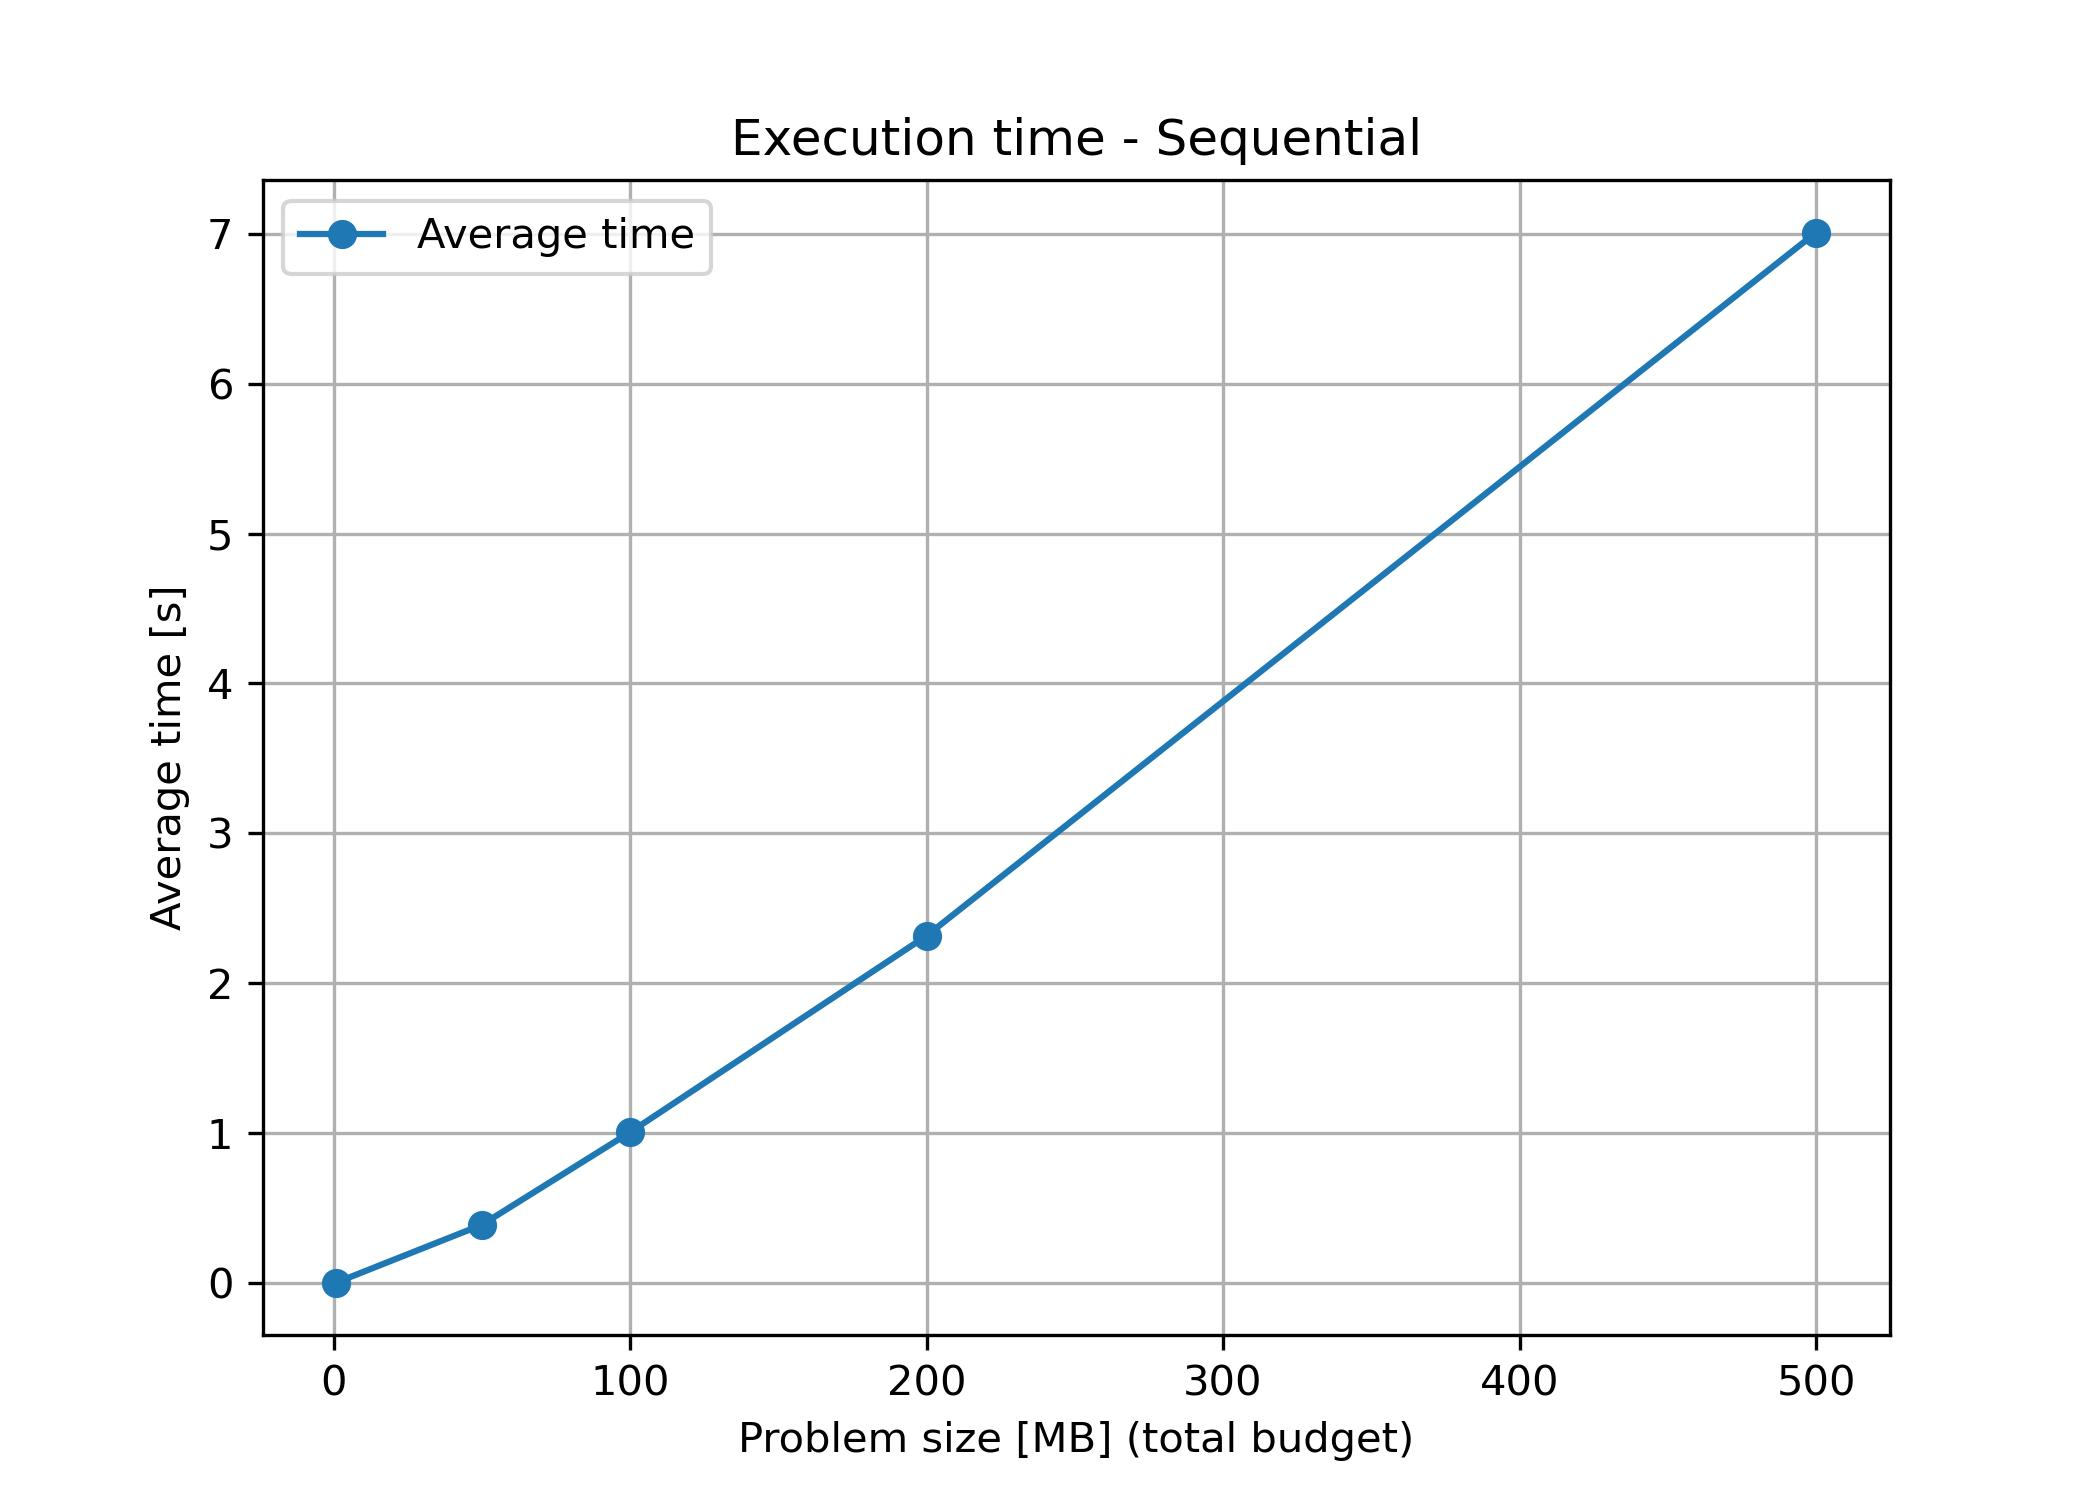
\includegraphics[width=1\linewidth]{img/seq_plots/seq_time.jpg}
				\caption{Tempi sequenziale}
				\label{fig:seq_time}
			\end{figure}
			
			\begin{figure}[H]
				\centering
				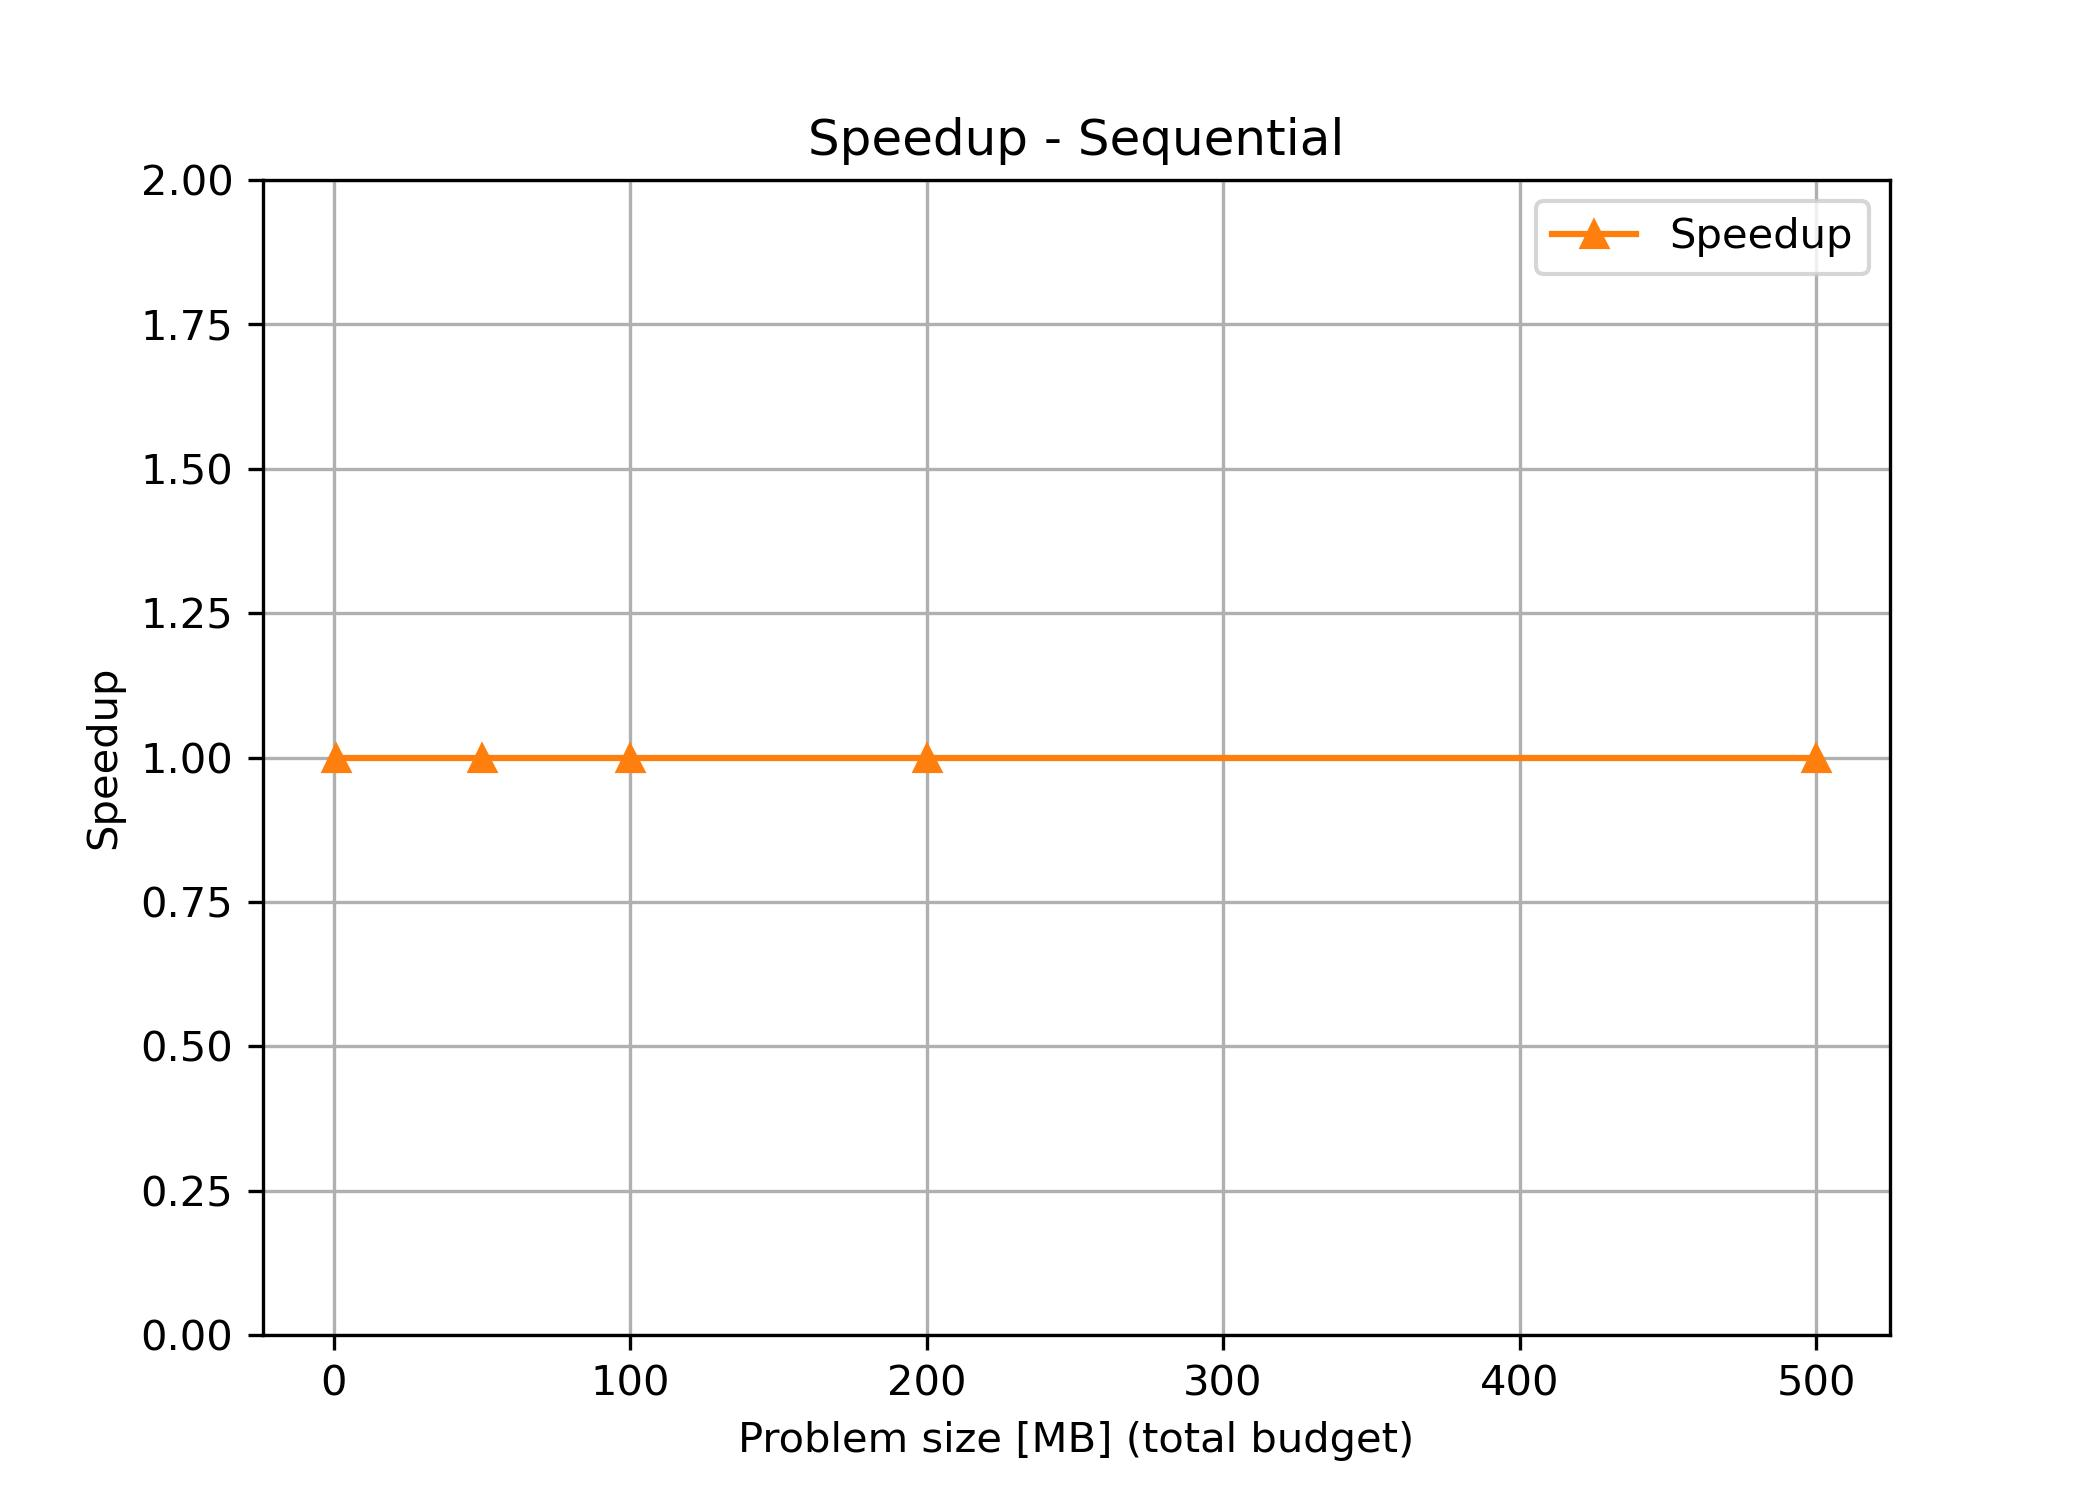
\includegraphics[width=1\linewidth]{img/seq_plots/seq_speedup.jpg}
				\caption{Speedup sequenziale}
				\label{fig:seq_speedup}
			\end{figure}
			
			\begin{figure}[H]
				\centering
				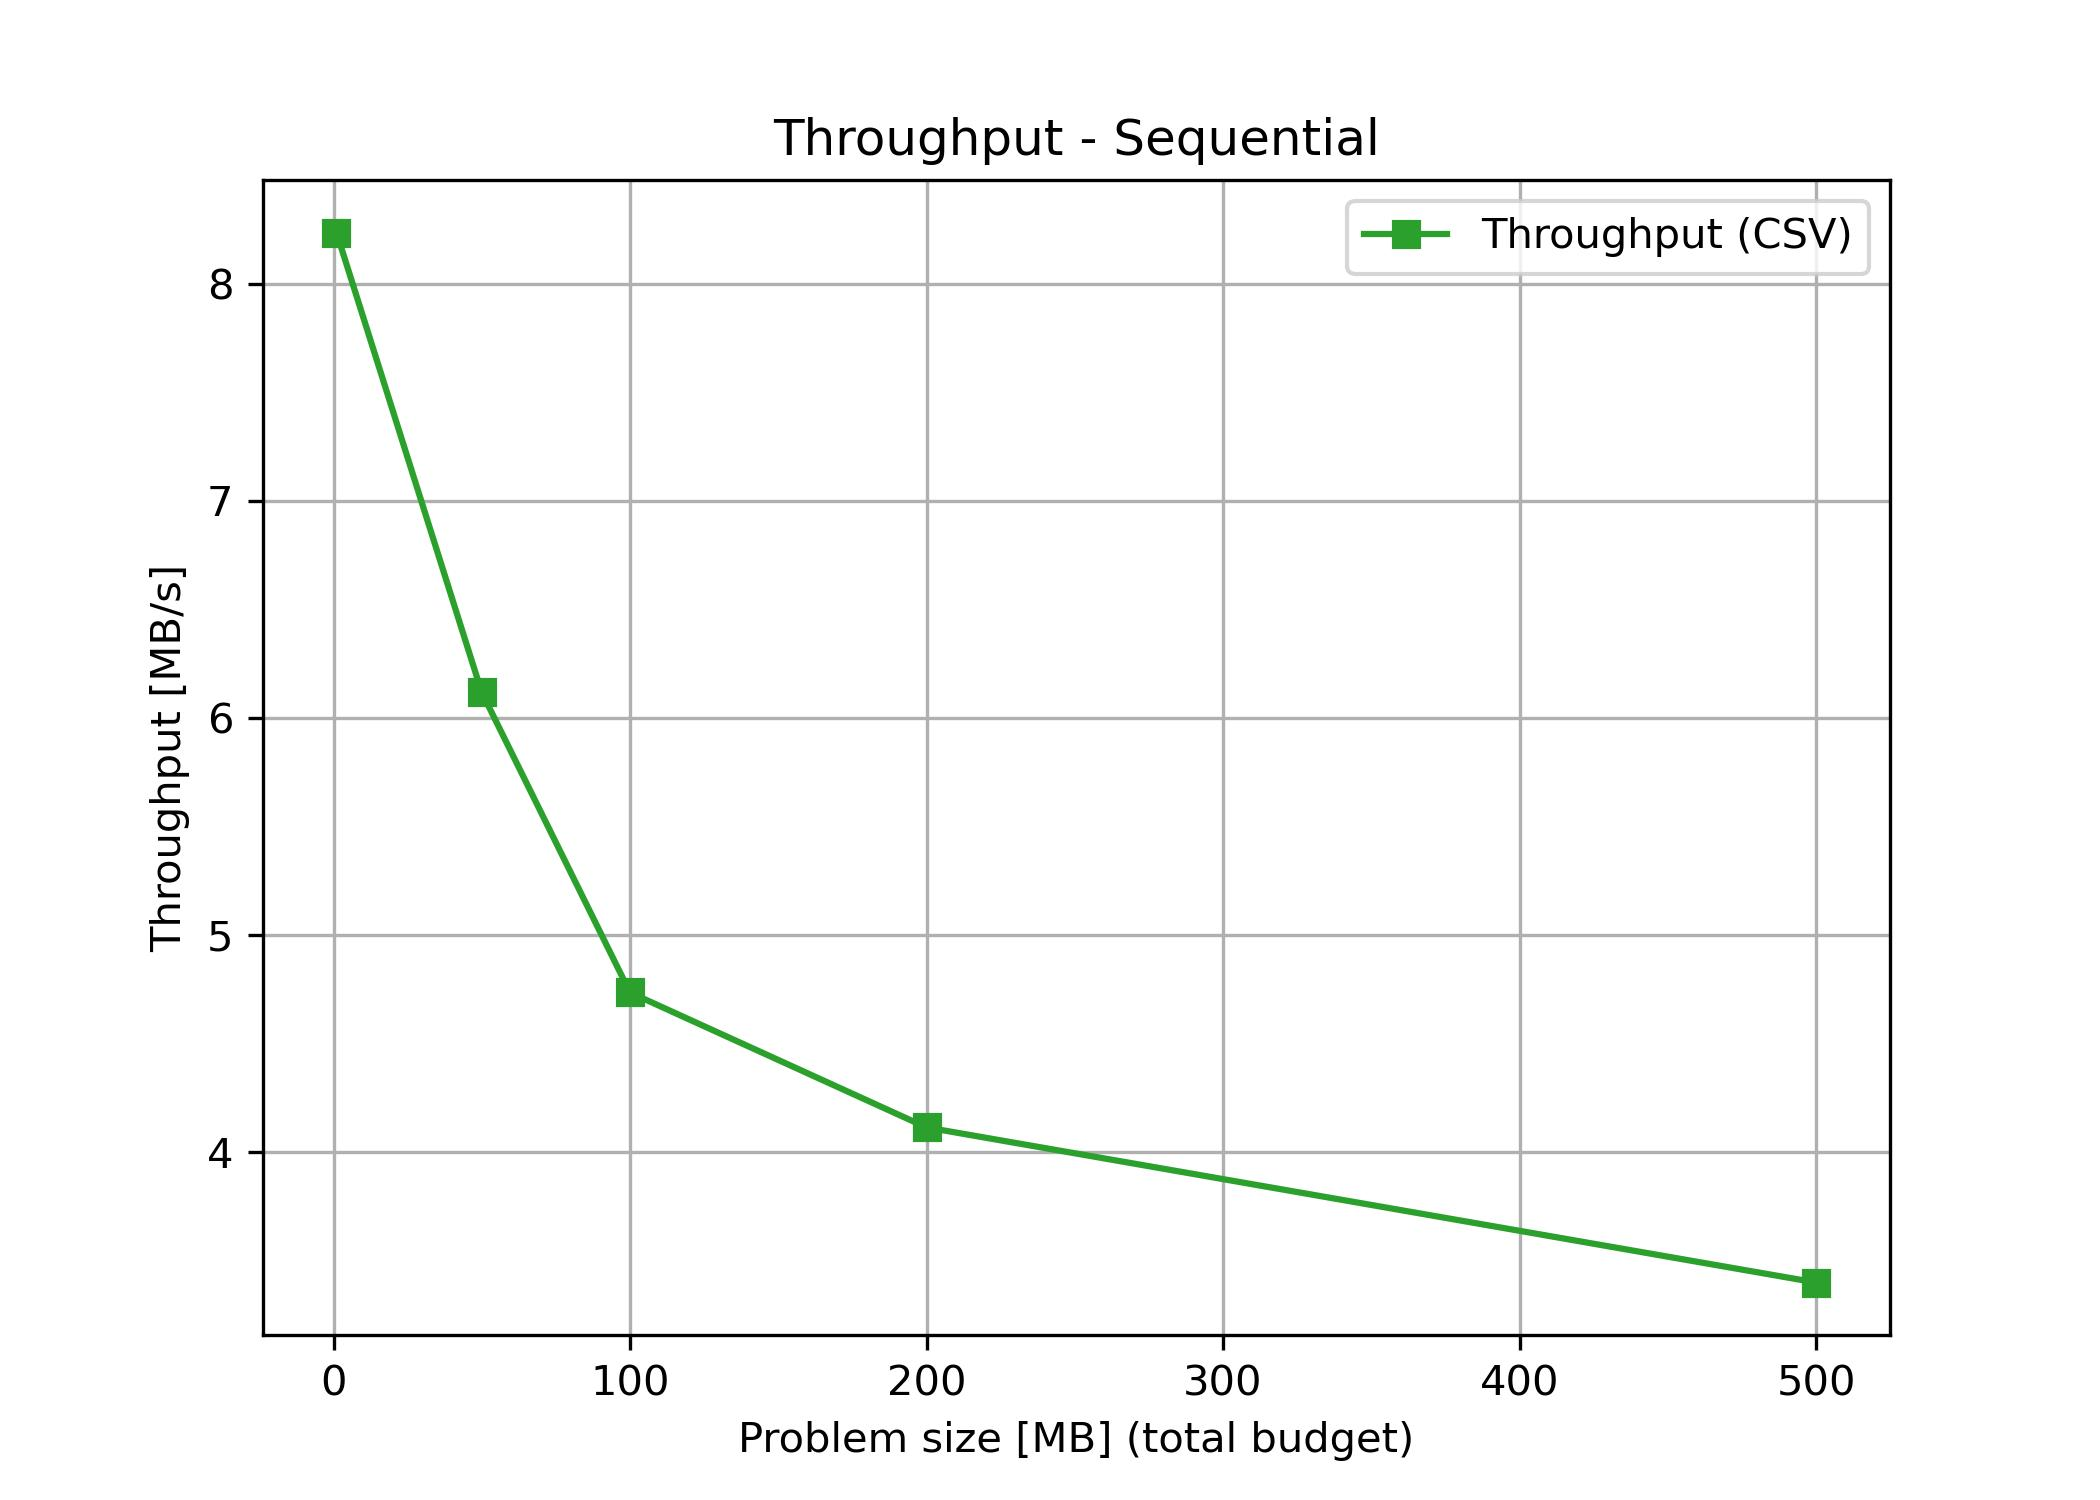
\includegraphics[width=1\linewidth]{img/seq_plots/seq_throughput.jpg}
				\caption{Throughput sequenziale}
				\label{fig:seq_throughput}
			\end{figure}
			
			\subsubsection*{Osservazioni}
				\begin{itemize}
						\item Il throughput decresce con la dimensione dell’input: da \(\sim 8.2\) MB/s (1 MB) a \(\sim 3.4\) MB/s (500 MB).
						\item La riduzione è coerente con la complessità \(O(n \log n)\) della costruzione SA, difatti all’aumentare di \(n\), il fattore logaritmico abbassa l’efficienza media.
						\item Per dataset piccoli, gli overhead fissi (\texttt{I/O}, allocazioni) pesano di più, causando un throughput apparente più elevato.
						\item La variabilità tra run è trascurabile ($<1$\% sui dataset grandi).
				\end{itemize}
		
		\subsection{Profiling della memoria}
			Il profiling della memoria è stato effettuato con \texttt{valgrind --tool=massif} sul dataset da 500 MB, producendo il file \texttt{seq\_500MB\_mem\_profile.txt}.
			Lo snapshot di picco riporta un consumo massimo di \(\sim 530\) MB, così suddivisi:
			\begin{enumerate}
				\item \(\sim 499\) MB (\(\sim 94\%\)) per i vettori \texttt{int} principali (\texttt{sa}, \texttt{rank}, \texttt{cnt}, \texttt{next}, \texttt{lcp});
				\item \(\sim 25\) MB (\(\sim 4.7\%\)) per il buffer \texttt{text};
				\item \(\sim 6.2\) MB (\(\sim 1.2\%\)) per i vettori booleani \texttt{bh}/\texttt{b2h}.
			\end{enumerate}
			
			\begin{figure}[H]
				\centering
				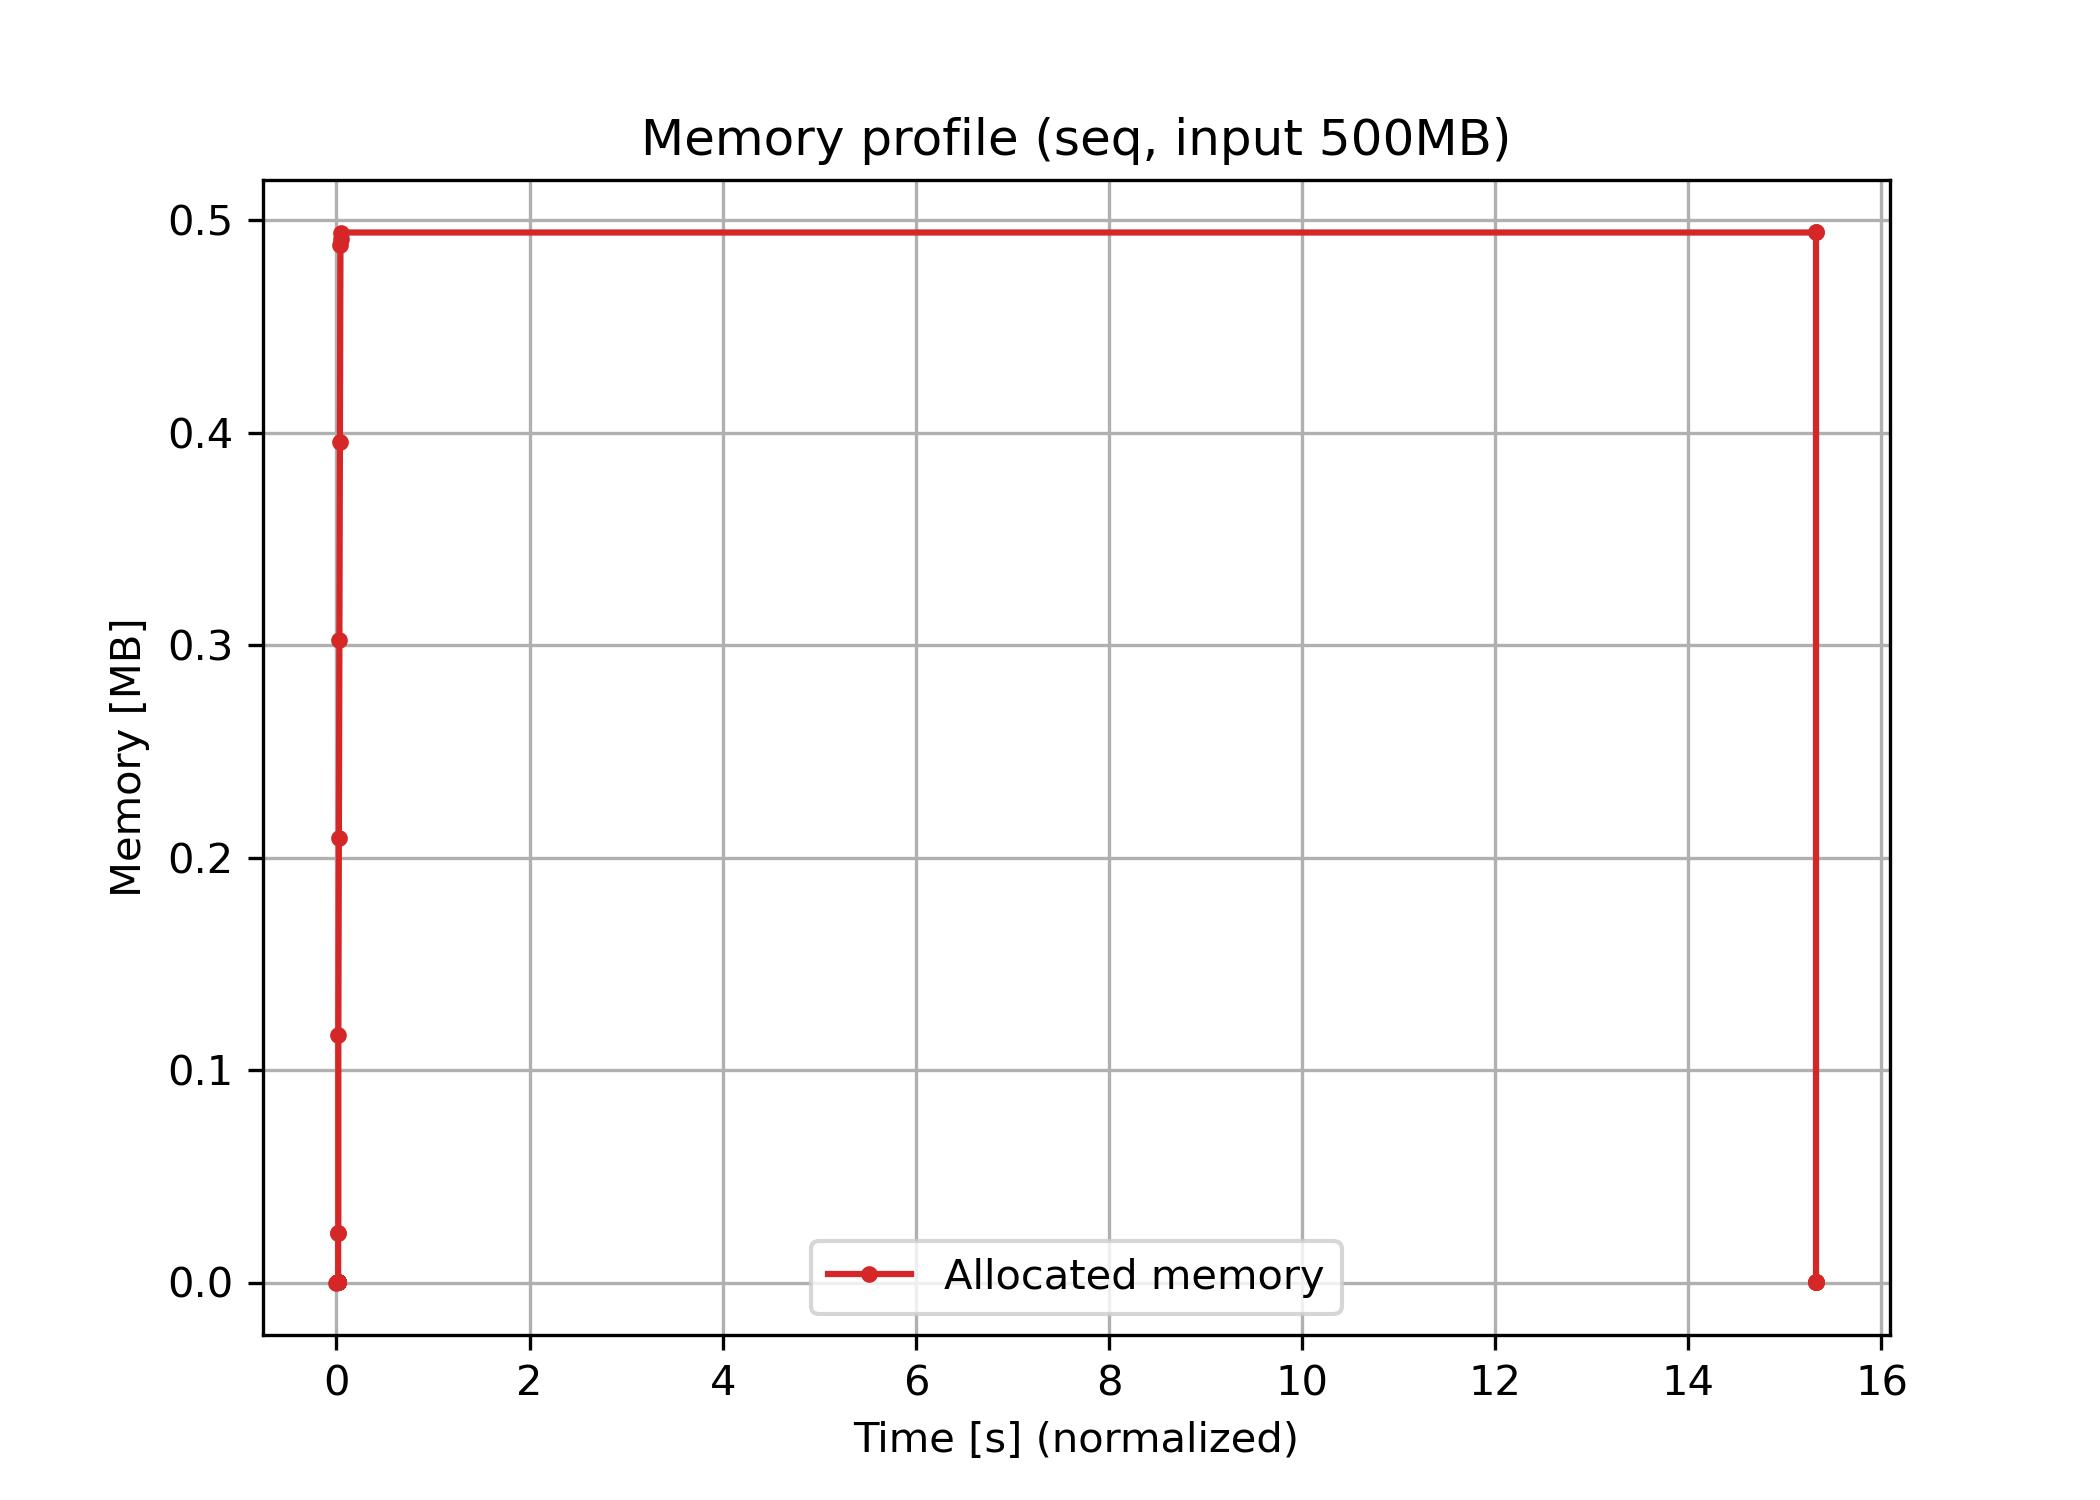
\includegraphics[width=1\linewidth]{img/seq_plots/seq_memory_profile.jpg}
				\caption{Memory usage sequenziale}
				\label{fig:seq_mem_usage}
			\end{figure}
			
			\subsubsection*{Confronto con l’analisi teorica}
				Nel WP1 era stato stimato un fabbisogno \(\approx 20n\) byte per i vettori di interi, più \(n\) byte per \texttt{text} e \(\frac{n}{4}\) byte per i vettori booleani.
				Per \(n=500\) MB il totale teorico atteso è \(\sim 530\) MB, perfettamente coerente con il picco misurato di \(\sim 530.6\) MB.
			
			\subsubsection*{Conclusione}
				La versione sequenziale evidenzia quindi un comportamento sia temporale che spaziale pienamente conforme all’analisi asintotica:
				prestazioni scalabili con \(n \log n\) e footprint di memoria dominato dai vettori ausiliari.
	
	\section{Versione OpenMP}
		
		\subsection{Analisi dei tempi}
			Le prestazioni sono state valutate con 2, 4 e 8 thread.
			I risultati medi su 10 run, ottenuti dai file \texttt{omp\_summary\_2.csv}, \texttt{omp\_summary\_4.csv} e \texttt{omp\_summary\_8.csv}, sono riportati nella Tabella~\ref{tab:omp-summary}.
			
			\begin{table}[H]
				\centering
				\begin{tabular}{|r|r|r|r|r|}
					\hline
					\textbf{Threads} & \textbf{Dimensione} & \textbf{Tempo medio [s]} & \textbf{Speedup} & \textbf{Efficienza [\%]} \\
					\hline
					2                     & 1 MB                & 0.0058                   & 1.12             & 56.2                     \\
					2                     & 50 MB               & 0.436                    & 0.95             & 47.7                     \\
					2                     & 100 MB              & 1.079                    & 0.98             & 48.8                     \\
					2                     & 200 MB              & 2.600                    & 0.92             & 46.1                     \\
					2                     & 500 MB              & 7.476                    & 0.96             & 48.2                     \\
					\hline
					4                     & 1 MB                & 0.0063                   & 1.02             & 25.5                     \\
					4                     & 50 MB               & 0.390                    & 1.07             & 26.7                     \\
					4                     & 100 MB              & 1.010                    & 1.04             & 26.0                     \\
					4                     & 200 MB              & 2.517                    & 0.95             & 23.8                     \\
					4                     & 500 MB              & 7.119                    & 1.01             & 25.3                     \\
					\hline
					8                     & 1 MB                & 0.0064                   & 1.02             & 12.7                     \\
					8                     & 50 MB               & 0.392                    & 1.06             & 13.3                     \\
					8                     & 100 MB              & 1.023                    & 1.03             & 12.9                     \\
					8                     & 200 MB              & 2.475                    & 0.97             & 12.1                     \\
					8                     & 500 MB              & 7.245                    & 1.00             & 12.4                     \\
					\hline
				\end{tabular}
				\caption{Risultati OpenMP (medie su 10 run): tempi, speedup ed efficienza.}
				\label{tab:omp-summary}
			\end{table}
			
			\begin{figure}[H]
				\centering
				\begin{minipage}[t]{0.49\textwidth}
					\centering
					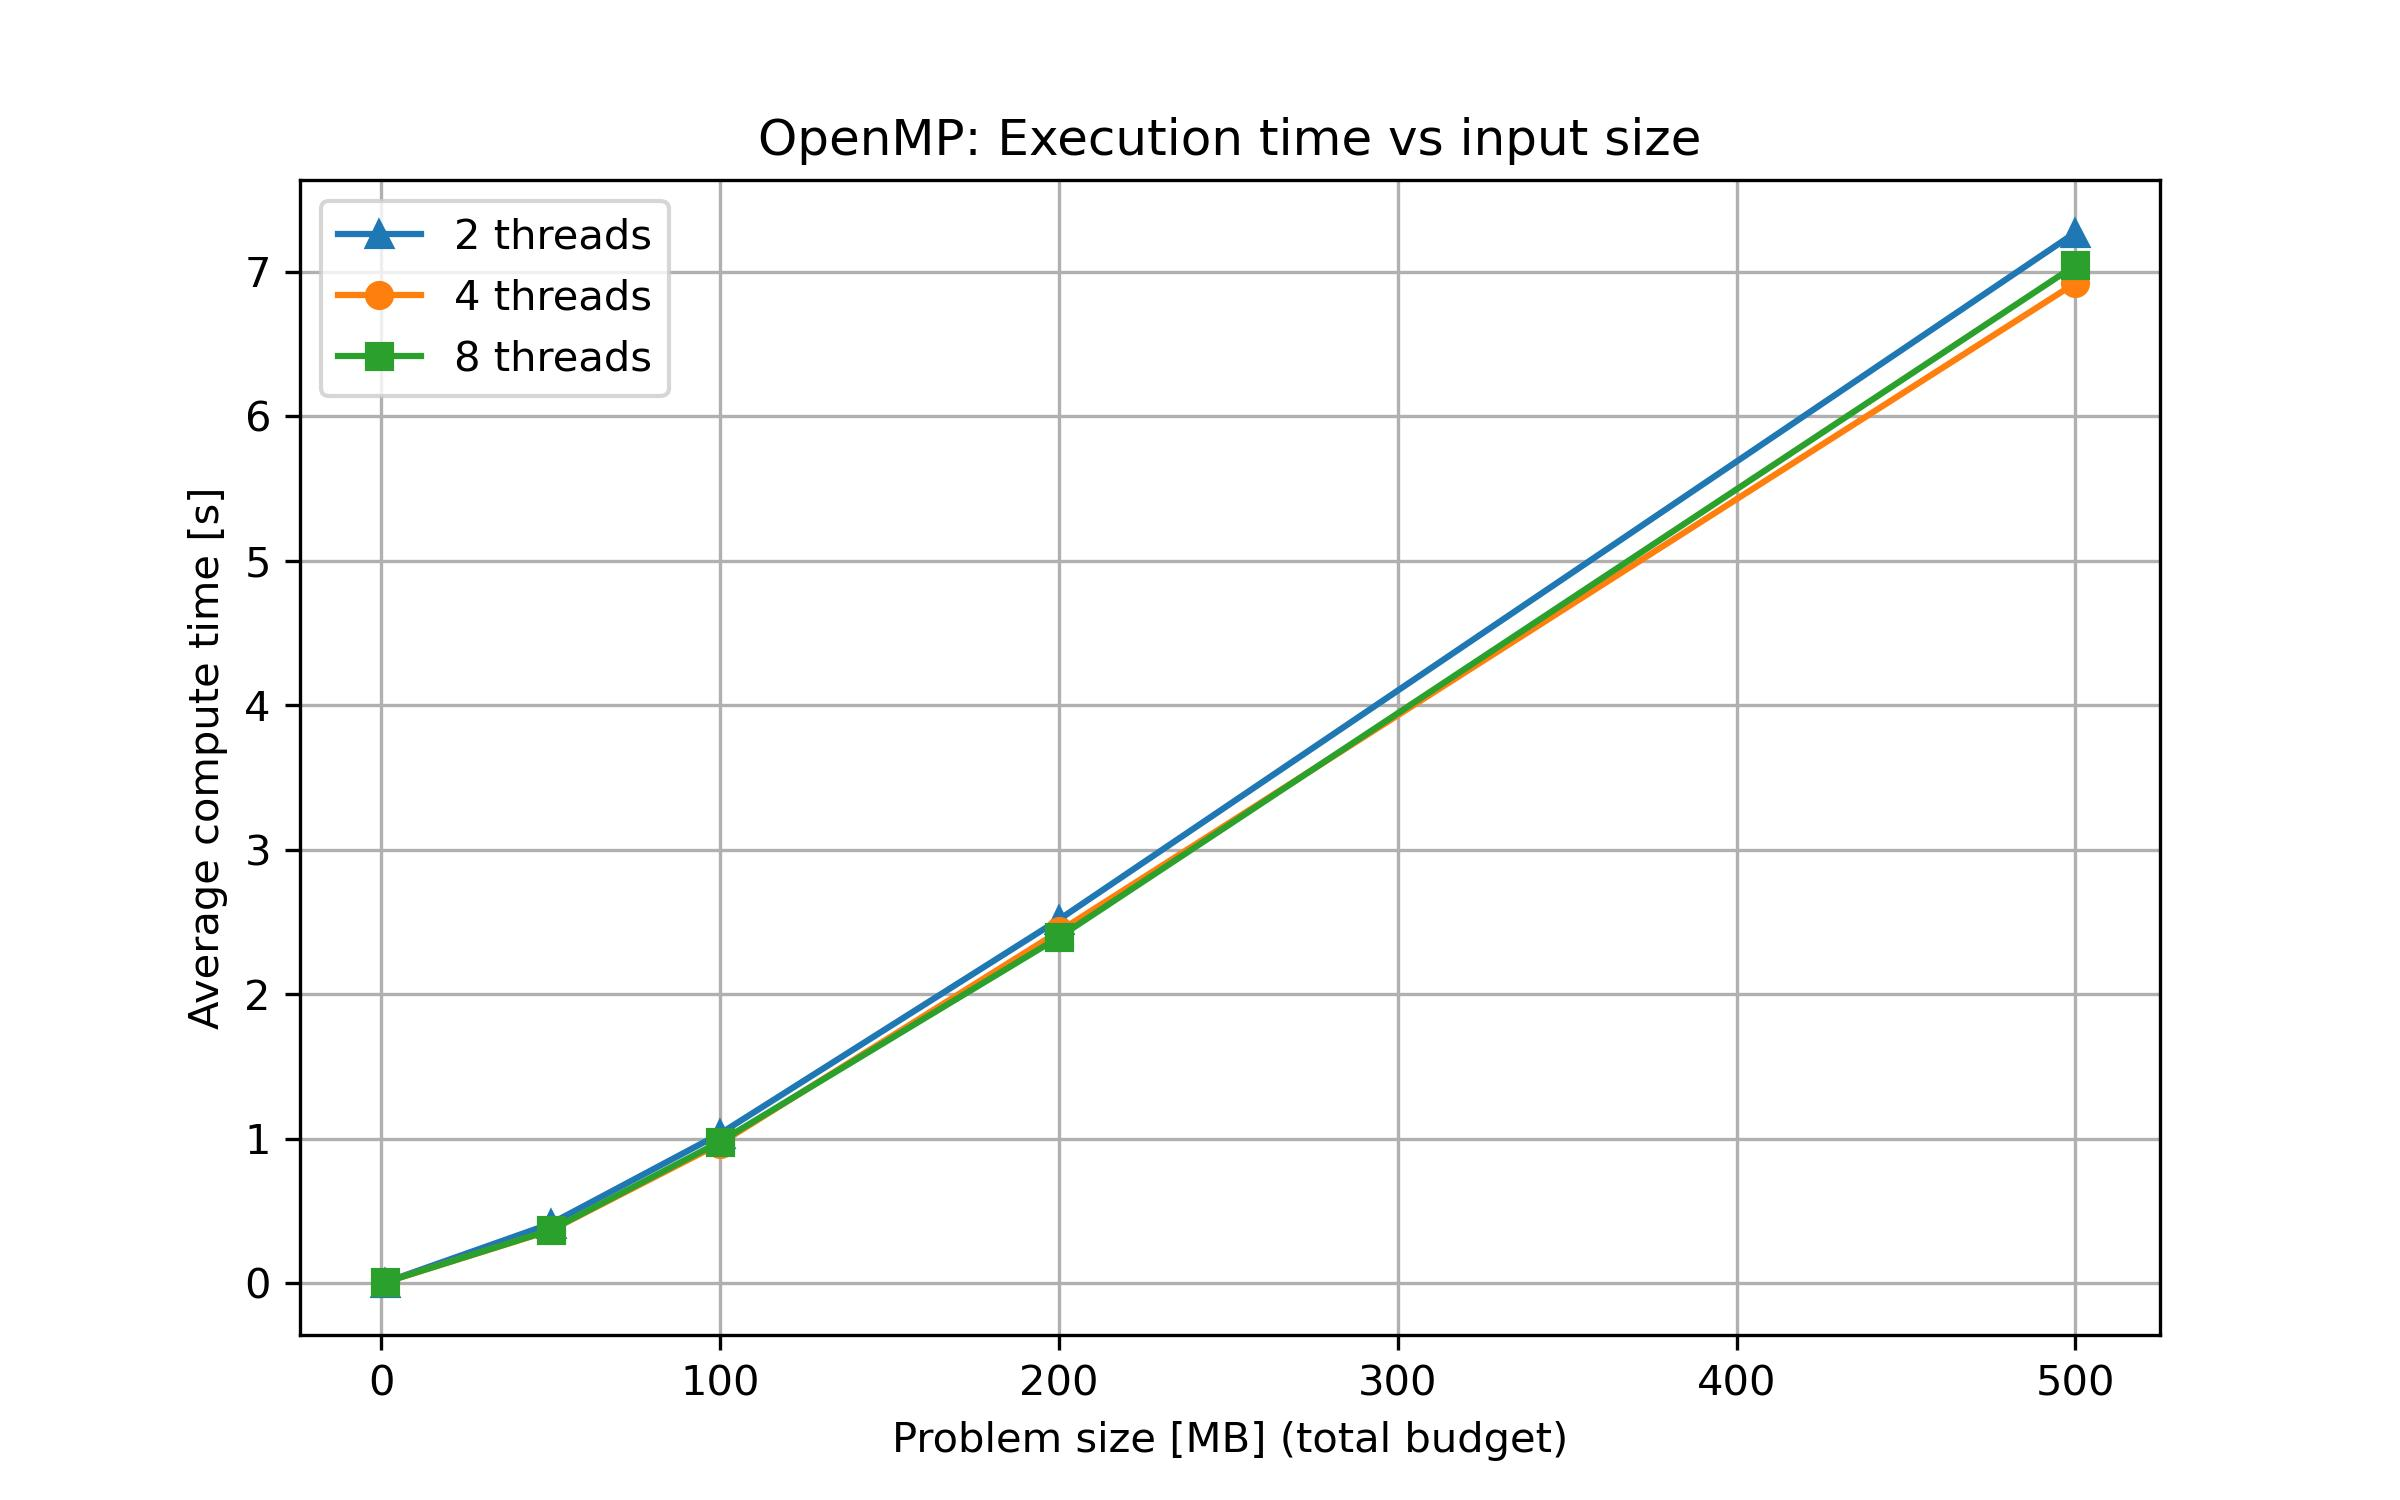
\includegraphics[width=\textwidth]{img/omp_plots/omp_times.jpg}
					\caption{Tempi OpenMP}
					\label{fig:omp_times}
				\end{minipage}
				\hfill
				\begin{minipage}[t]{0.49\textwidth}
					\centering
					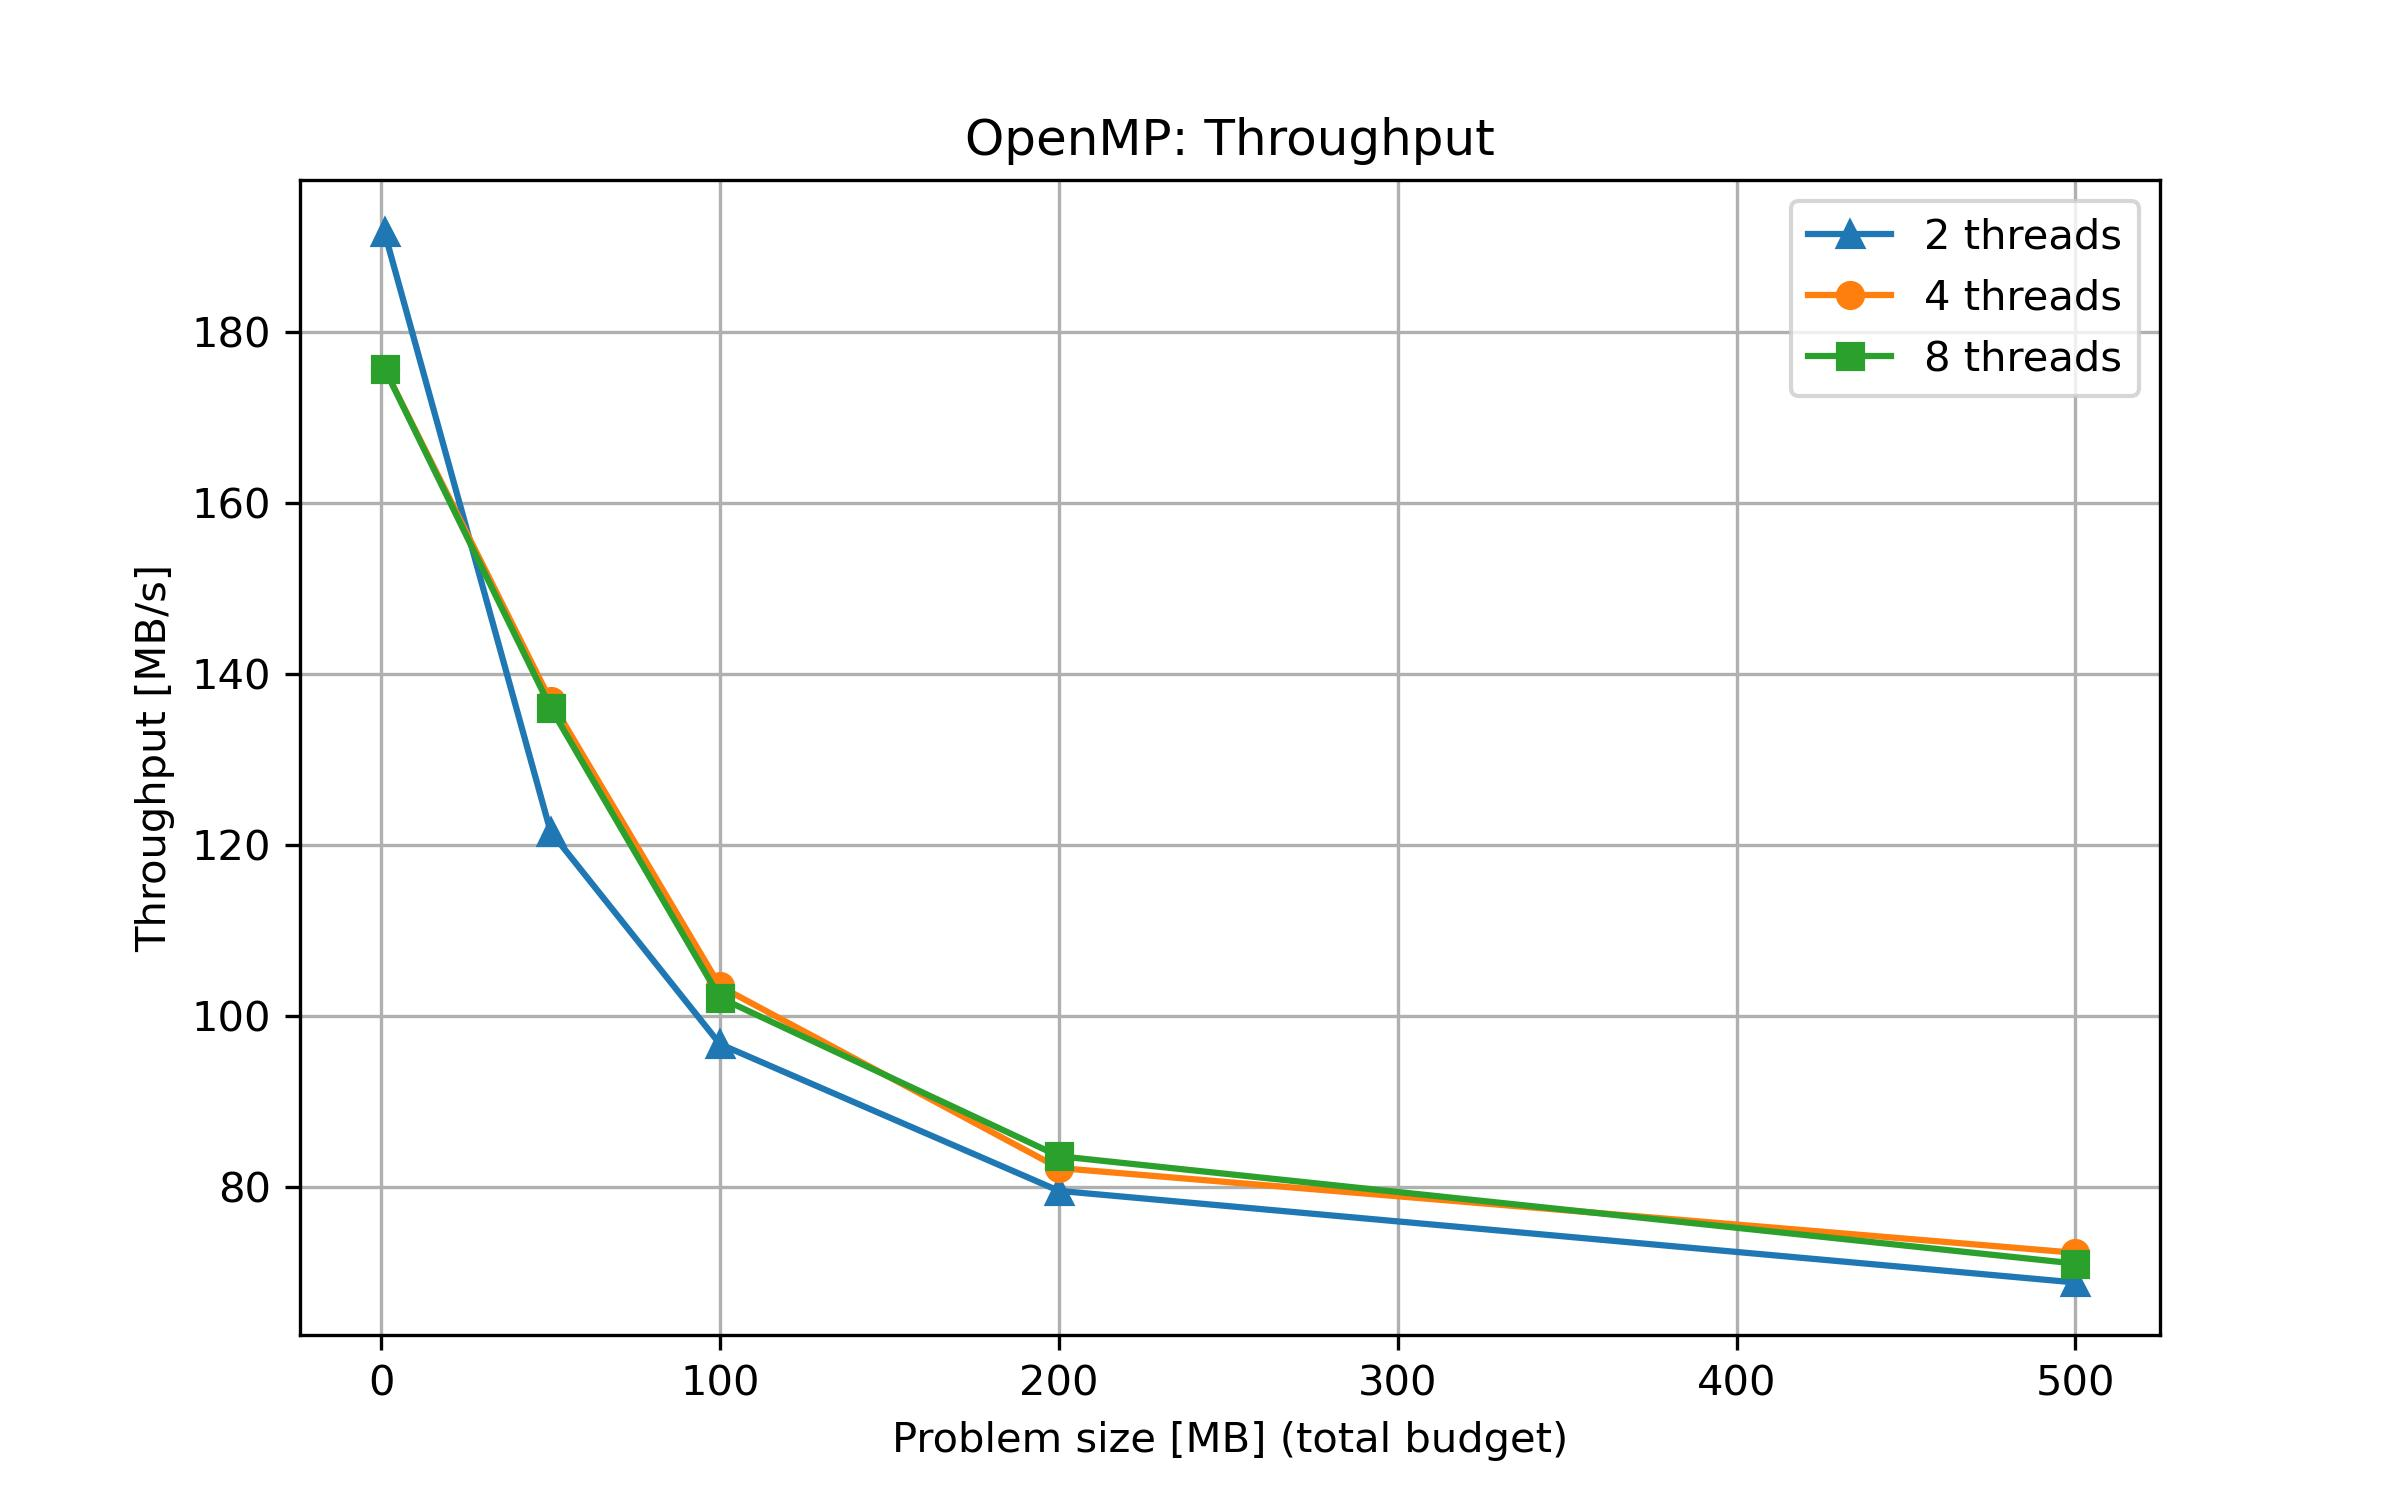
\includegraphics[width=\textwidth]{img/omp_plots/omp_throughput.jpg}
					\caption{Throughput OpenMP}
					\label{fig:omp_throughput}
				\end{minipage}
			\end{figure}
			
			\begin{figure}[H]
				\centering
				\begin{minipage}[t]{0.49\textwidth}
					\centering
					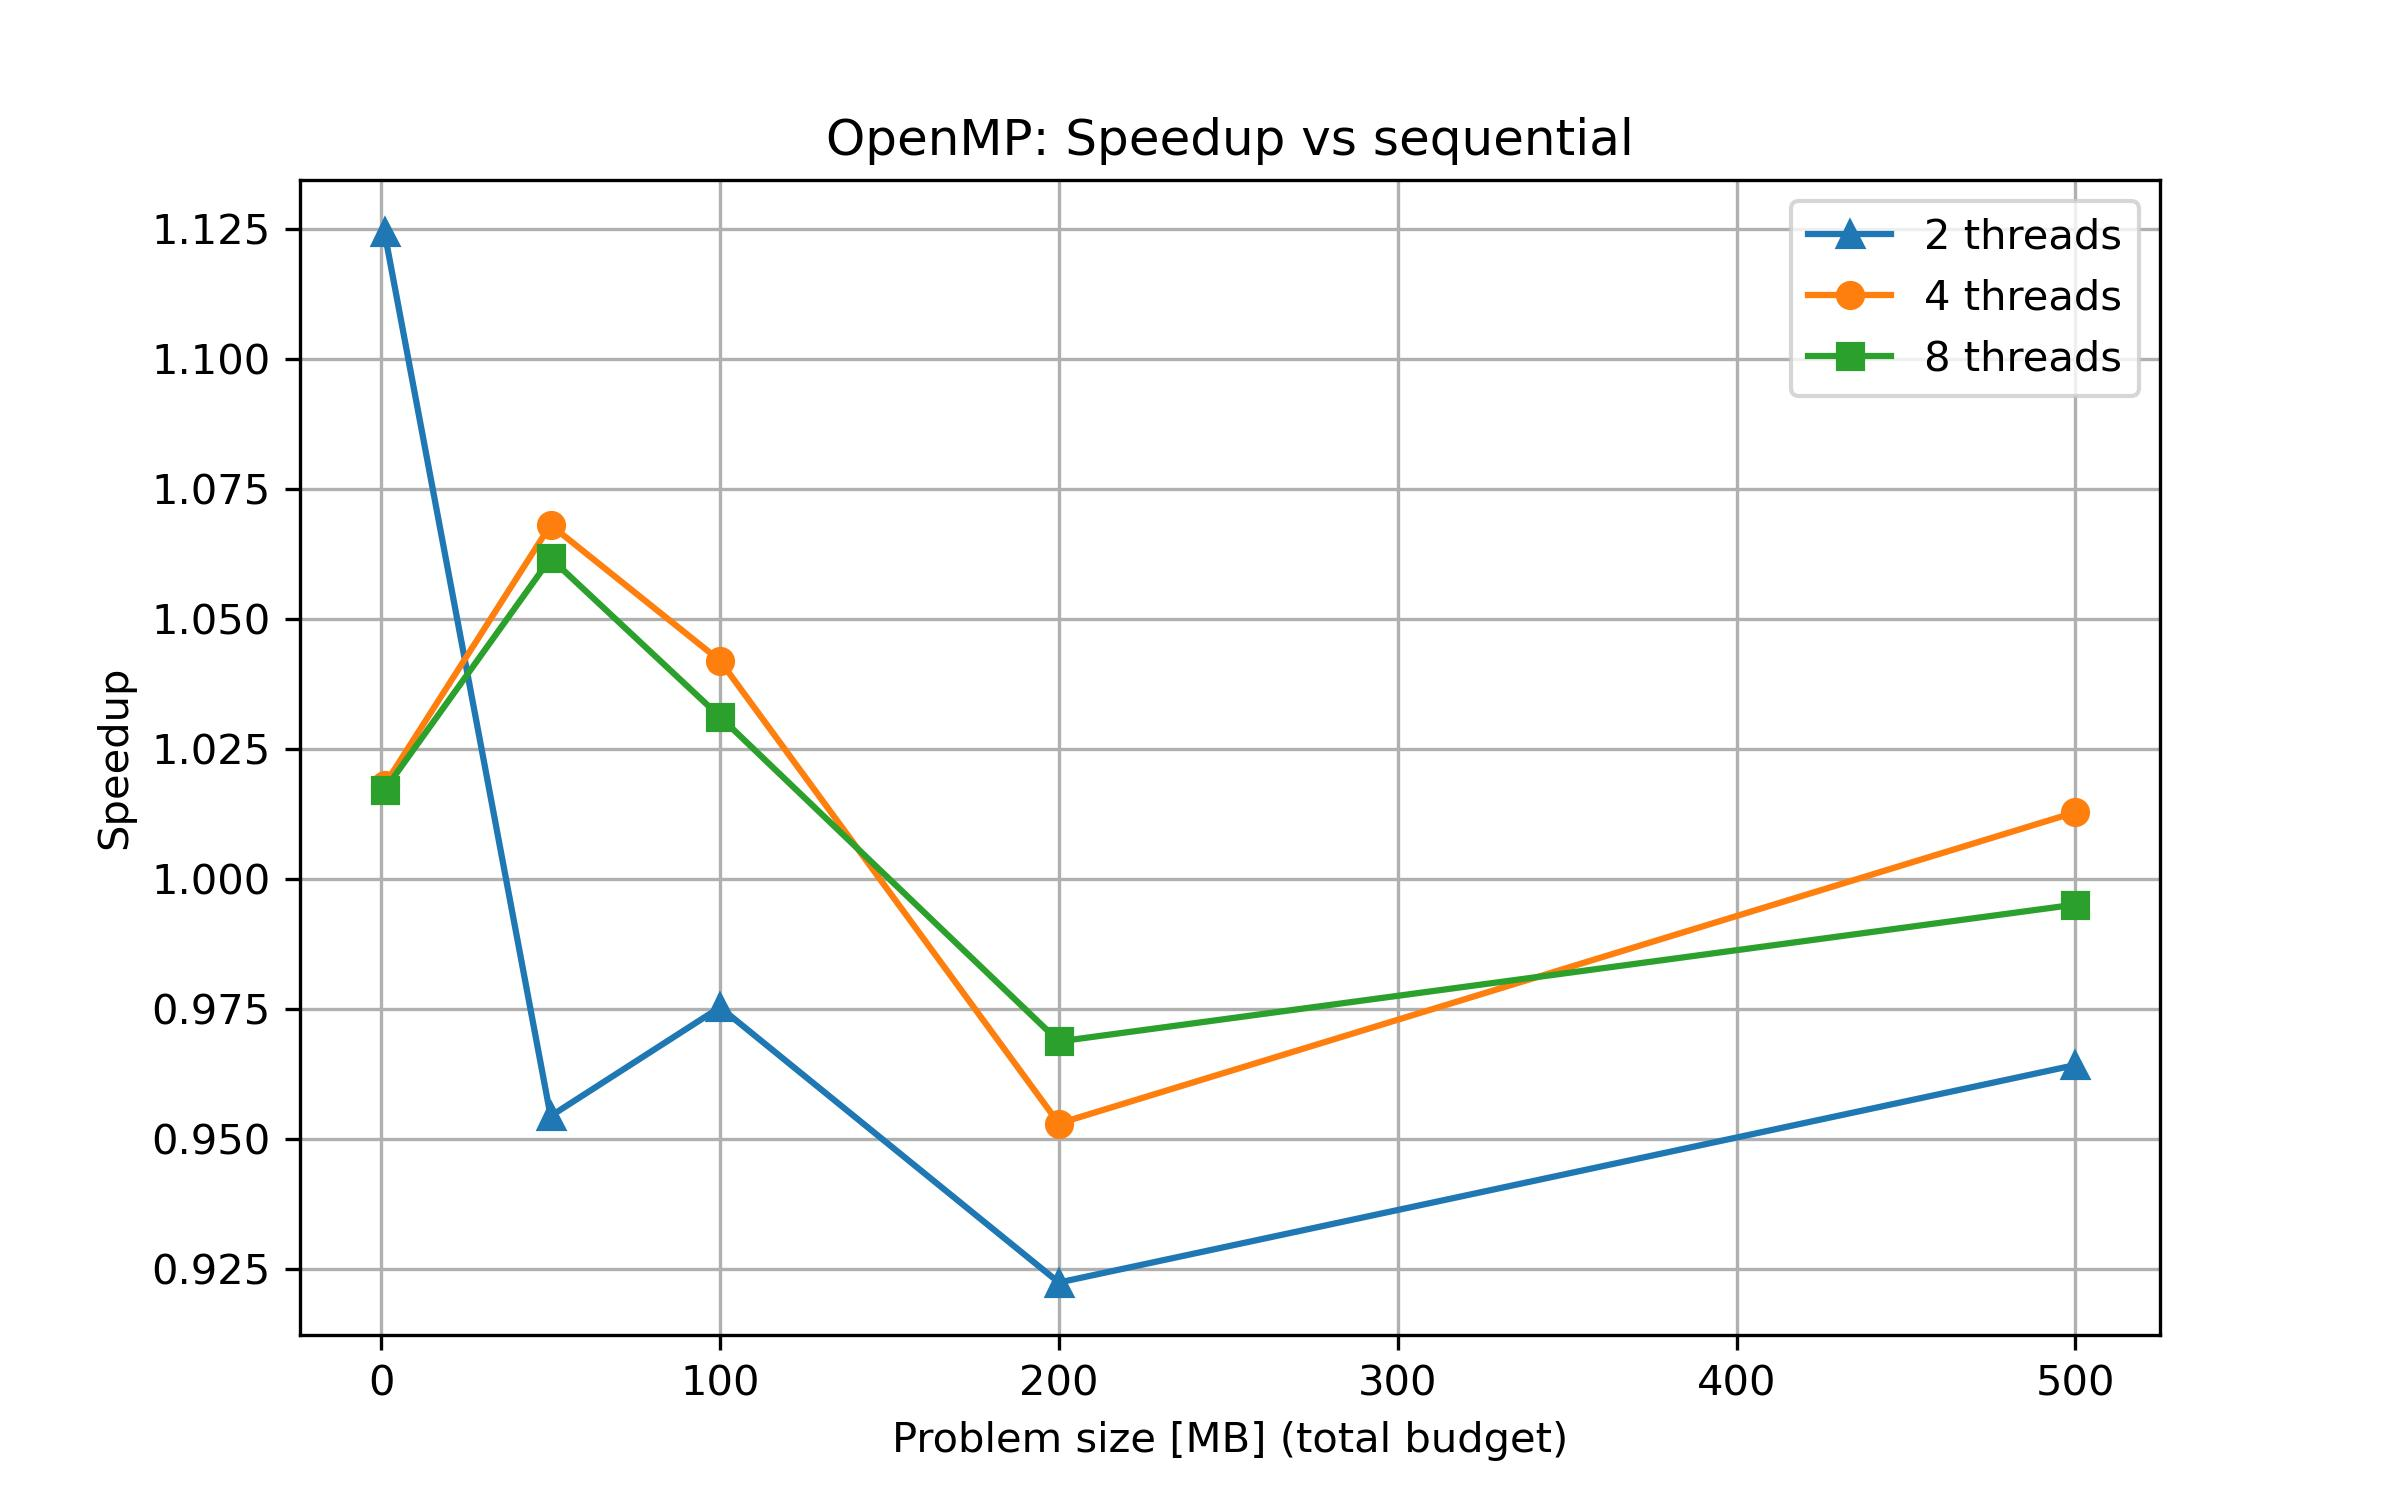
\includegraphics[width=\textwidth]{img/omp_plots/omp_speedup.jpg}
					\caption{Speedup OpenMP}
					\label{fig:omp_speedup}
				\end{minipage}
				\hfill
				\begin{minipage}[t]{0.49\textwidth}
					\centering
					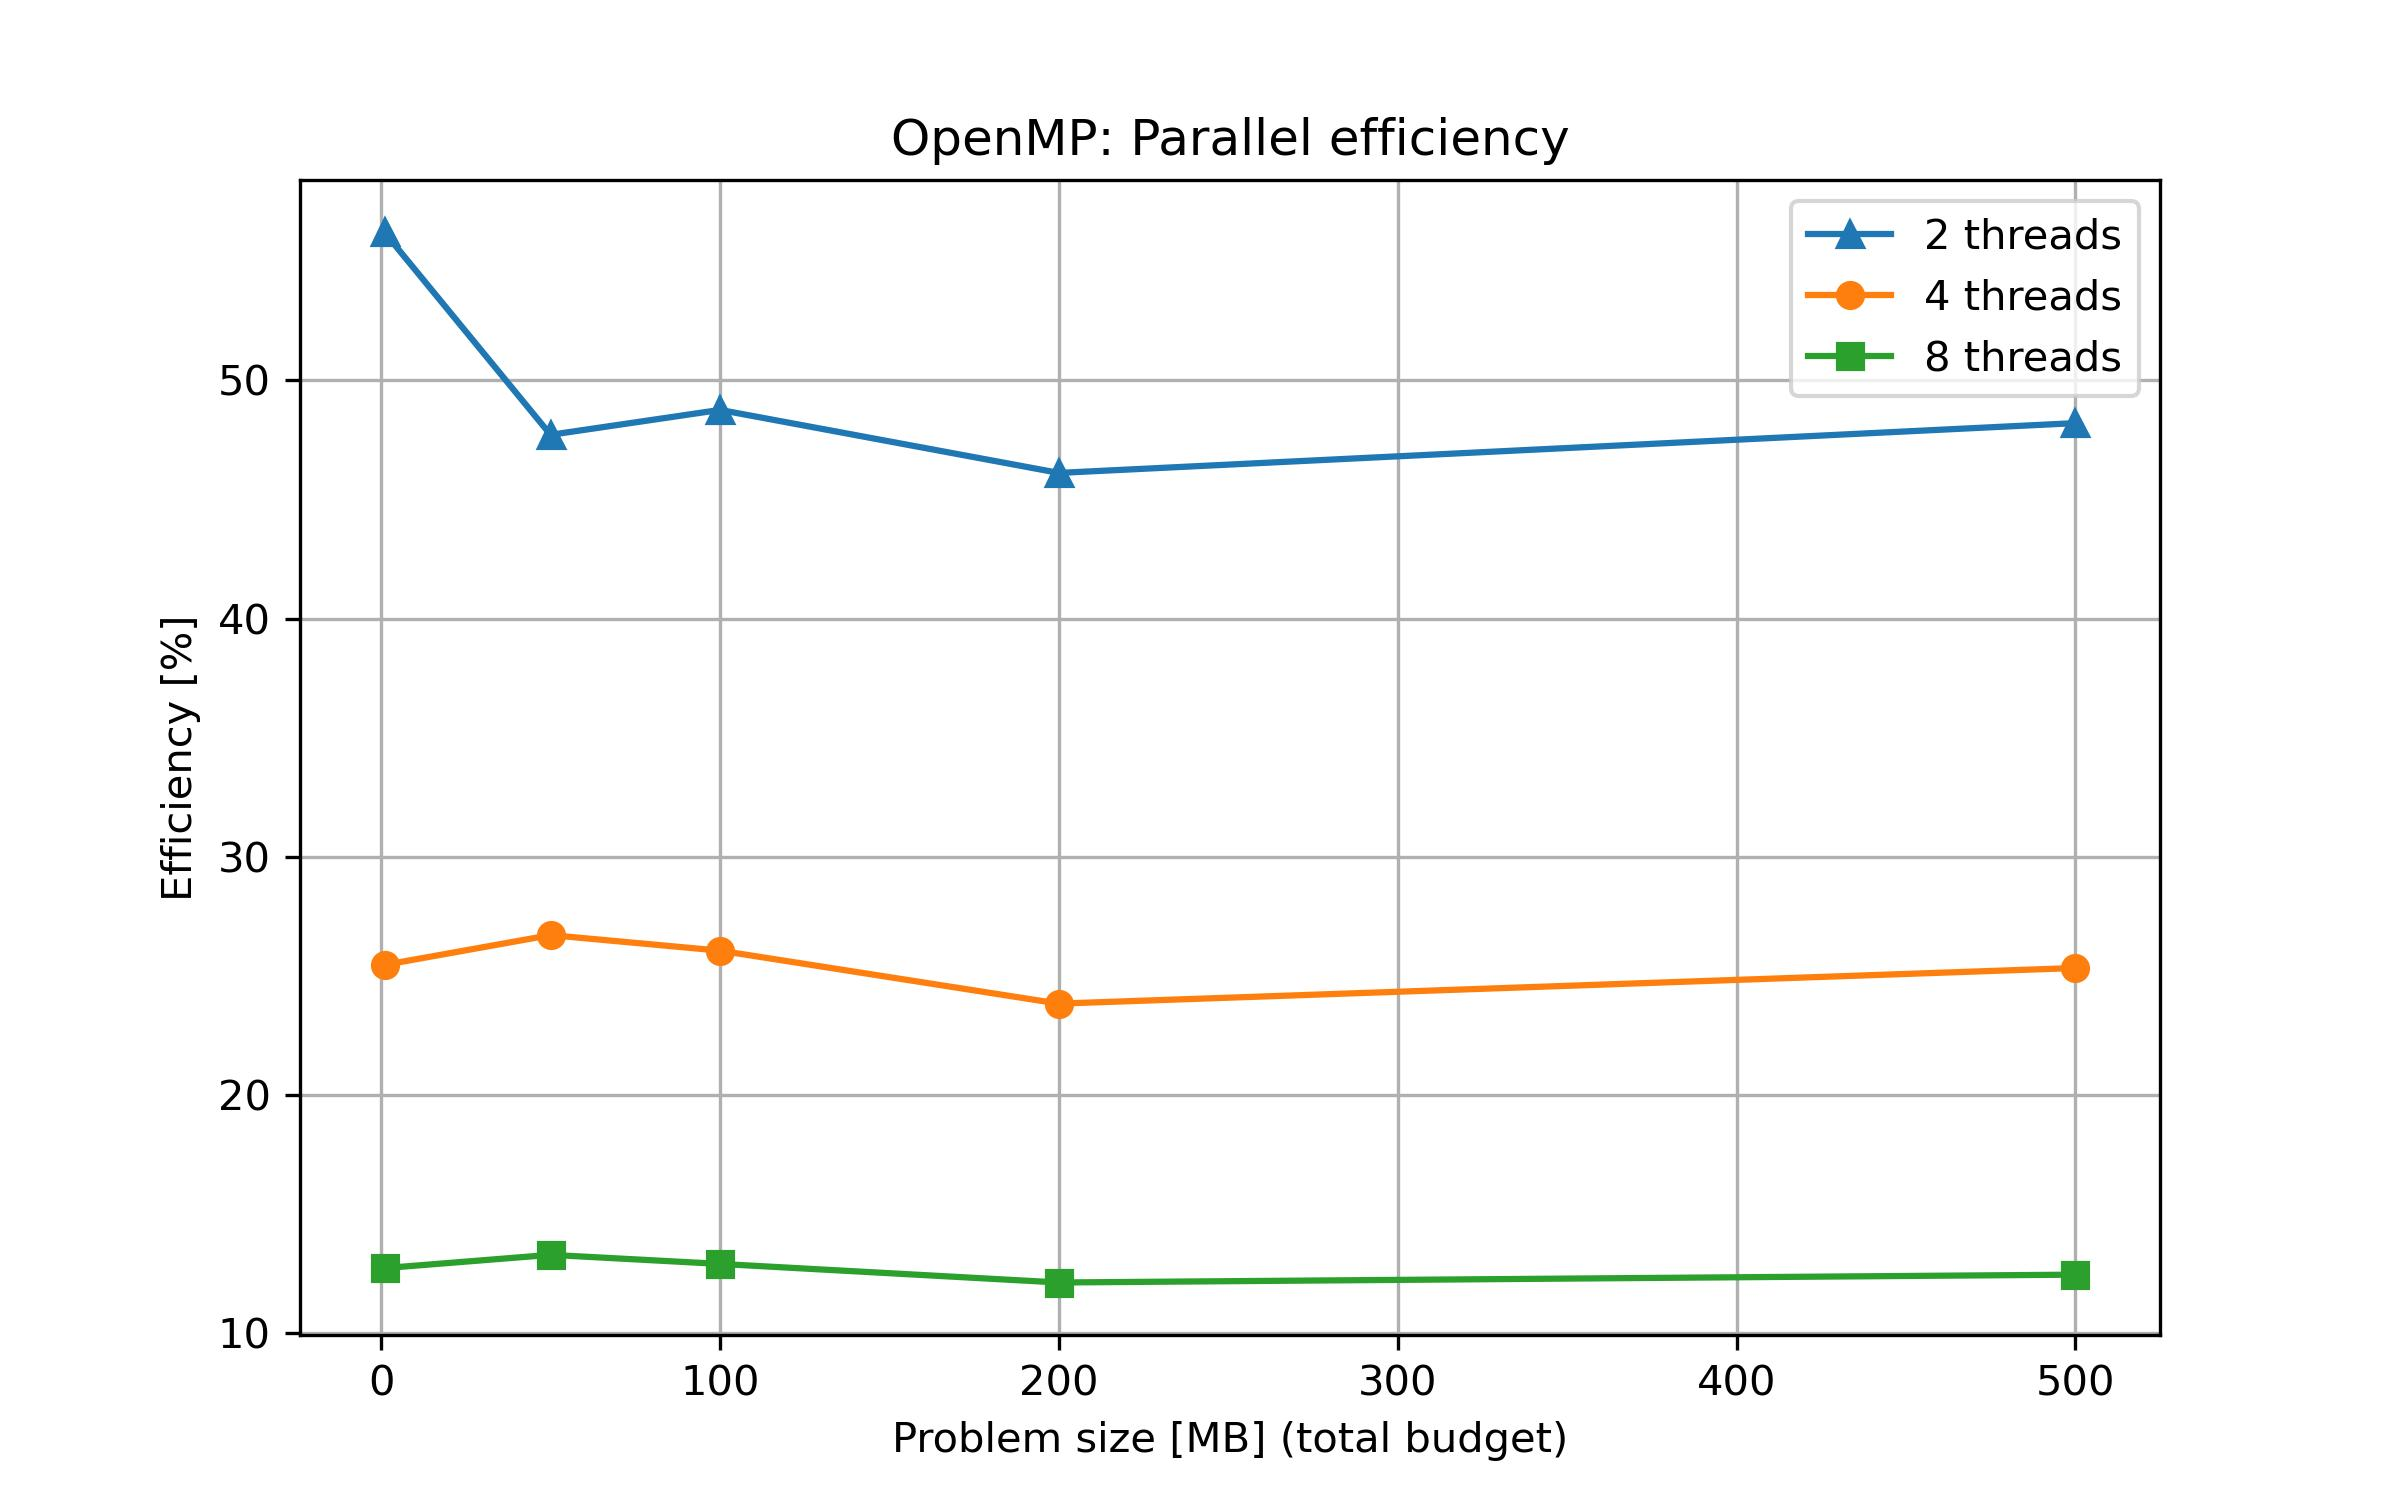
\includegraphics[width=\textwidth]{img/omp_plots/omp_efficiency.jpg}
					\caption{Efficiency OpenMP}
					\label{fig:omp_efficiency}
				\end{minipage}
			\end{figure}
			
			\subsubsection*{Osservazioni}
				\begin{itemize}
						\item Con 2 thread si osserva in media un lieve degrado rispetto al sequenziale (speedup $\sim$0.95--0.98$\times$ su dataset grandi).
						\item Con 4 thread lo speedup raggiunge al massimo $\sim$1.07$\times$, con efficienza intorno al 25\%.
						\item Con 8 thread le prestazioni non migliorano ulteriormente: lo speedup resta $\sim$1.0--1.03$\times$ e l’efficienza scende sotto il 13\%.
						\item L’implementazione OpenMP mostra quindi un guadagno prestazionale molto limitato, penalizzato da colli di bottiglia di memoria e sezioni sequenziali non parallelizzate.
				\end{itemize}
		
		\subsection{Profiling della memoria}
			Il profiling con \texttt{valgrind --tool=massif} è stato eseguito su input da 500 MB (\texttt{seq\_omp\_2t\_500MB\_mem\_profile.txt}, \texttt{seq\_omp\_4t\_500MB\_mem\_profile.txt}, \texttt{seq\_omp\_8t\_500MB\_mem\_profile.txt}).
			In tutti i casi, il picco massimo si attesta intorno a \textbf{530 MB}, così suddivisi:
			\begin{itemize}
				\item $\sim$499 MB (94\%) per i vettori \texttt{int} principali (\texttt{sa}, \texttt{rank}, \texttt{cnt}, \texttt{next}, \texttt{lcp});
				\item $\sim$25 MB (4.7\%) per il buffer \texttt{text};
				\item $\sim$6 MB (1.2\%) per i vettori booleani \texttt{bh}/\texttt{b2h}.
			\end{itemize}
			
			\subsubsection*{Confronto 2 vs 4 vs 8 thread}
				\begin{itemize}
						\item I profili di memoria risultano praticamente identici: OpenMP non introduce copie ulteriori dei buffer, ma lavora sugli stessi dati condivisi.
						\item L’unica differenza rilevabile è un leggero incremento nello stack per i thread aggiuntivi, trascurabile rispetto al footprint complessivo.
				\end{itemize}
				
				\begin{figure}[H]
						\centering
						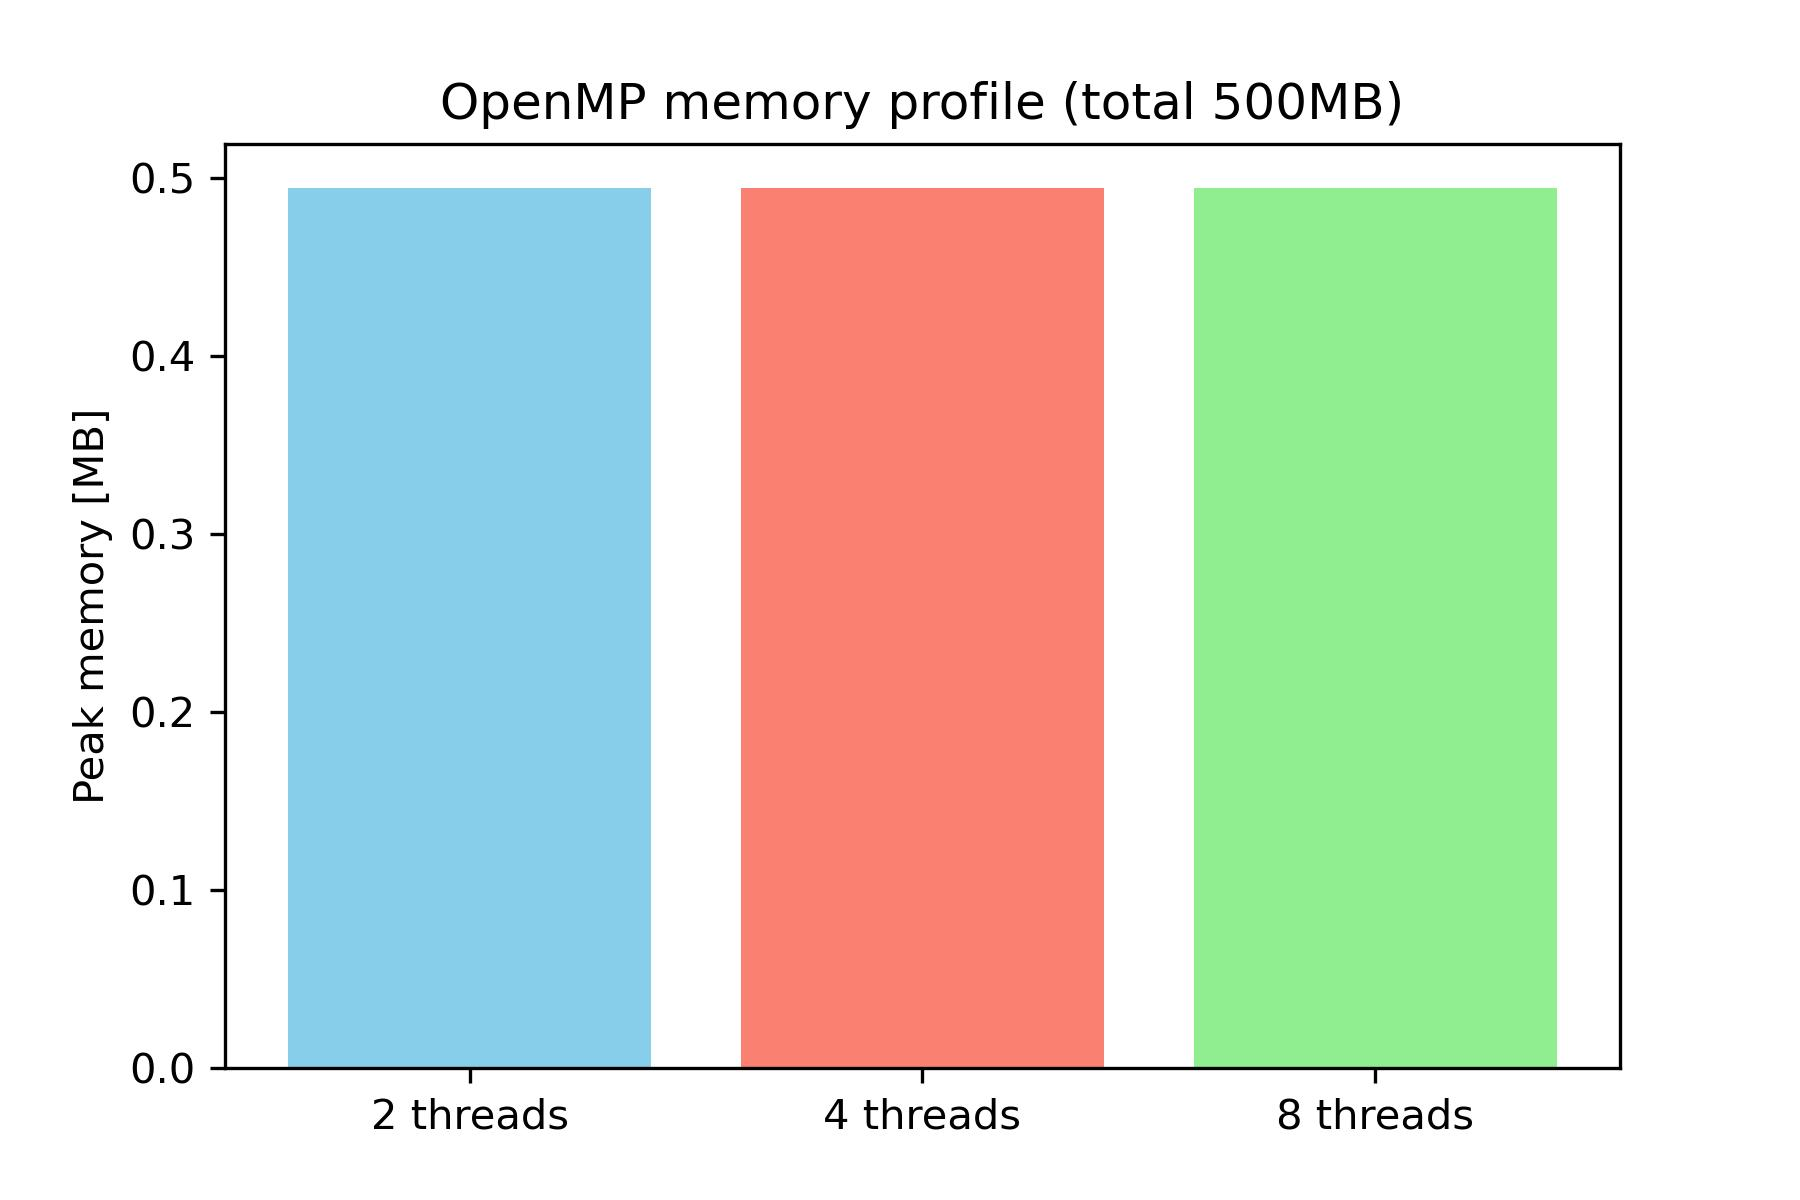
\includegraphics[width=1\linewidth]{img/omp_plots/omp_memory.jpg}
						\caption{Memory usage OpenMP (500 MB)}
						\label{fig:omp_mem_usage}
				\end{figure}
			
			\subsubsection*{Conclusione}
				L’uso di OpenMP non riduce il fabbisogno di memoria rispetto al sequenziale, mentre i benefici sui tempi sono molto contenuti.
				Lo speedup resta nell’intervallo $0.95\text{--}1.07\times$ con efficienza bassa, segno che la natura dell’algoritmo e l’accesso irregolare ai dati non si prestano bene alla parallelizzazione a memoria condivisa.
	
	\section{Versione MPI}
		
		\subsection{Analisi dei tempi}
			Le prestazioni della versione distribuita sono state valutate con 10 run per ciascun dataset
			\(\{1, 50, 100, 200, 500\}\,\)MB e per tre configurazioni di ranks (\(2,4,8\)).
			I risultati medi (\texttt{mpi\_summary\_2.csv}, \texttt{mpi\_summary\_4.csv}, \texttt{mpi\_summary\_8.csv})
			sono riassunti nella Tabella~\ref{tab:mpi-summary}.
			
			\begin{table}[H]
				\centering
				\begin{tabular}{|r|r|r|r|r|}
					\hline
					\textbf{Ranks} & \textbf{Dimensione} & \textbf{Tempo medio [s]} & \textbf{Speedup} & \textbf{Efficienza [\%]} \\
					\hline
					2                   & 1 MB                & 0.0049                   & 1.19             & 59.6                     \\
					2                   & 50 MB               & 0.4481                   & 0.87             & 43.6                     \\
					2                   & 100 MB              & 0.9678                   & 1.04             & 52.1                     \\
					2                   & 200 MB              & 2.2857                   & 1.02             & 50.8                     \\
					2                   & 500 MB              & 6.9496                   & 1.01             & 50.5                     \\
					\hline
					4                   & 1 MB                & 0.0037                   & 1.56             & 39.0                     \\
					4                   & 50 MB               & 0.3219                   & 1.21             & 30.3                     \\
					4                   & 100 MB              & 0.7201                   & 1.40             & 35.0                     \\
					4                   & 200 MB              & 1.6010                   & 1.45             & 36.2                     \\
					4                   & 500 MB              & 5.5493                   & 1.26             & 31.6                     \\
					\hline
					8                   & 1 MB                & 0.0034                   & 1.71             & 21.3                     \\
					8                   & 50 MB               & 0.2743                   & 1.42             & 17.8                     \\
					8                   & 100 MB              & 0.6112                   & 1.65             & 20.6                     \\
					8                   & 200 MB              & 1.4090                   & 1.65             & 20.6                     \\
					8                   & 500 MB              & 4.9807                   & 1.41             & 17.6                     \\
					\hline
				\end{tabular}
				\caption{Risultati MPI (medie su 10 run): tempi, speedup ed efficienza.}
				\label{tab:mpi-summary}
			\end{table}
			
			\begin{figure}[H]
				\centering
				\begin{minipage}[t]{0.49\textwidth}
					\centering
					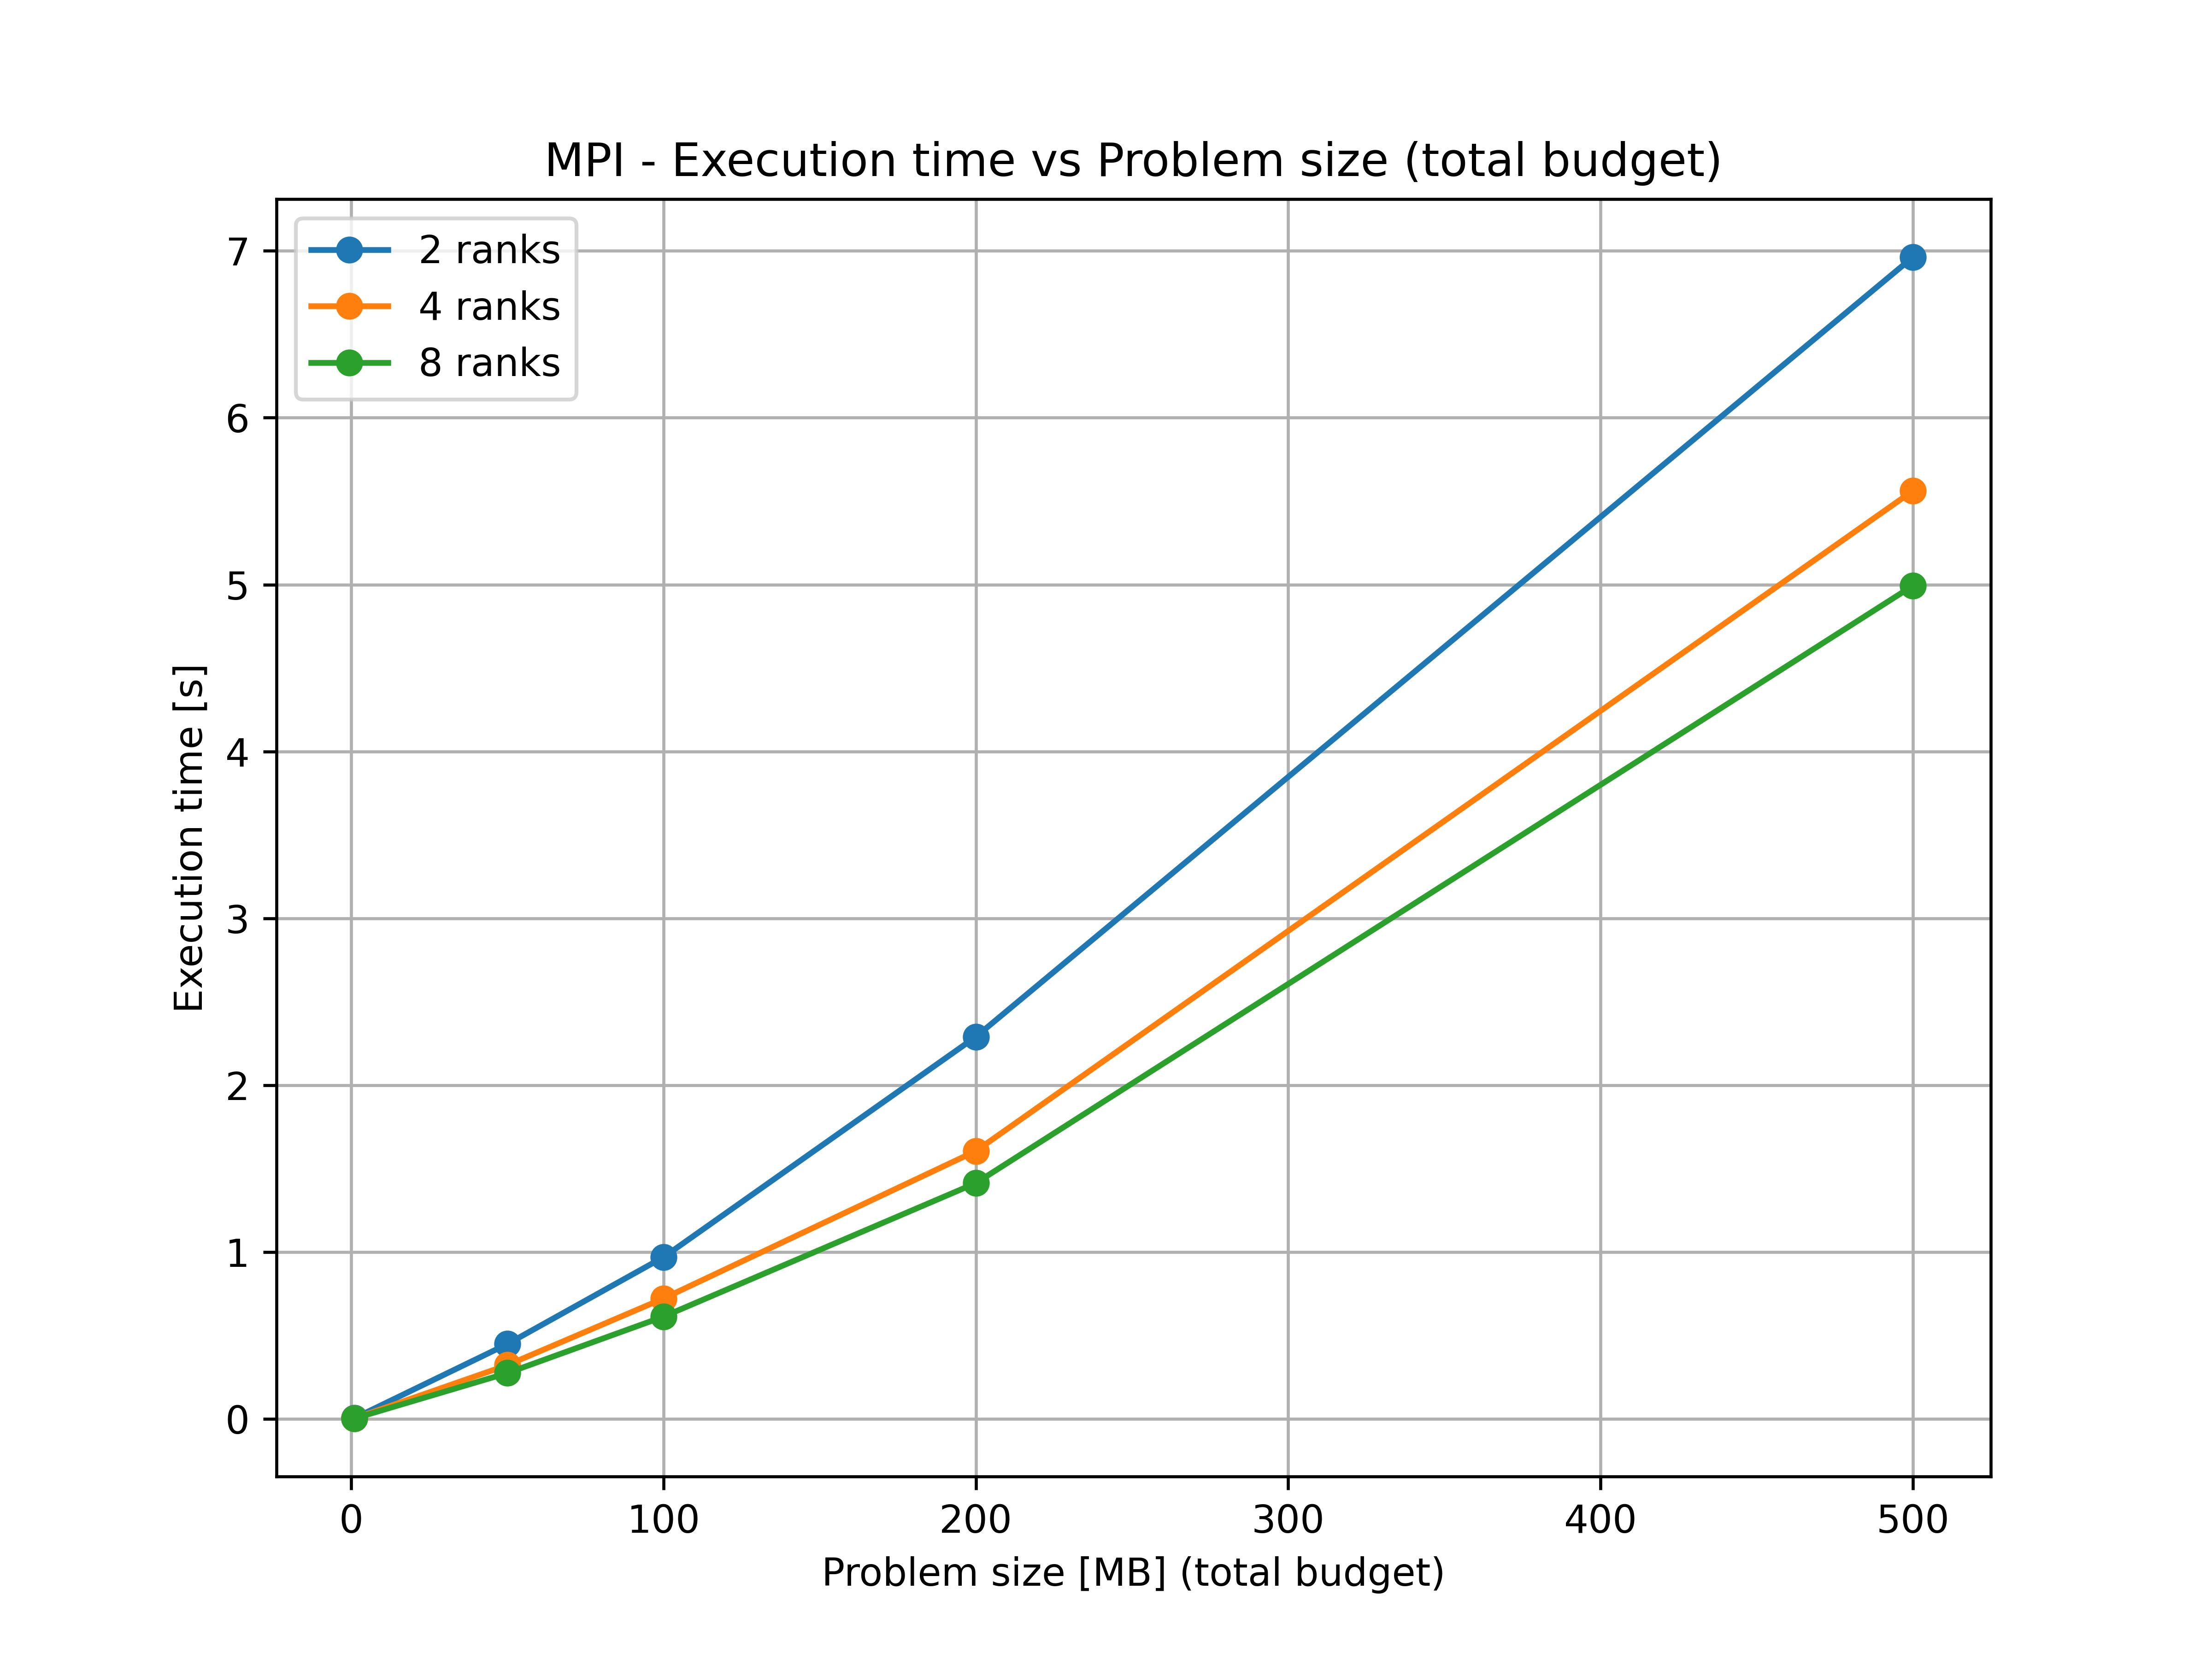
\includegraphics[width=\textwidth]{img/mpi_plots/mpi_times.jpg}
					\caption{Tempi MPI}
					\label{fig:mpi_times}
				\end{minipage}
				\hfill
				\begin{minipage}[t]{0.49\textwidth}
					\centering
					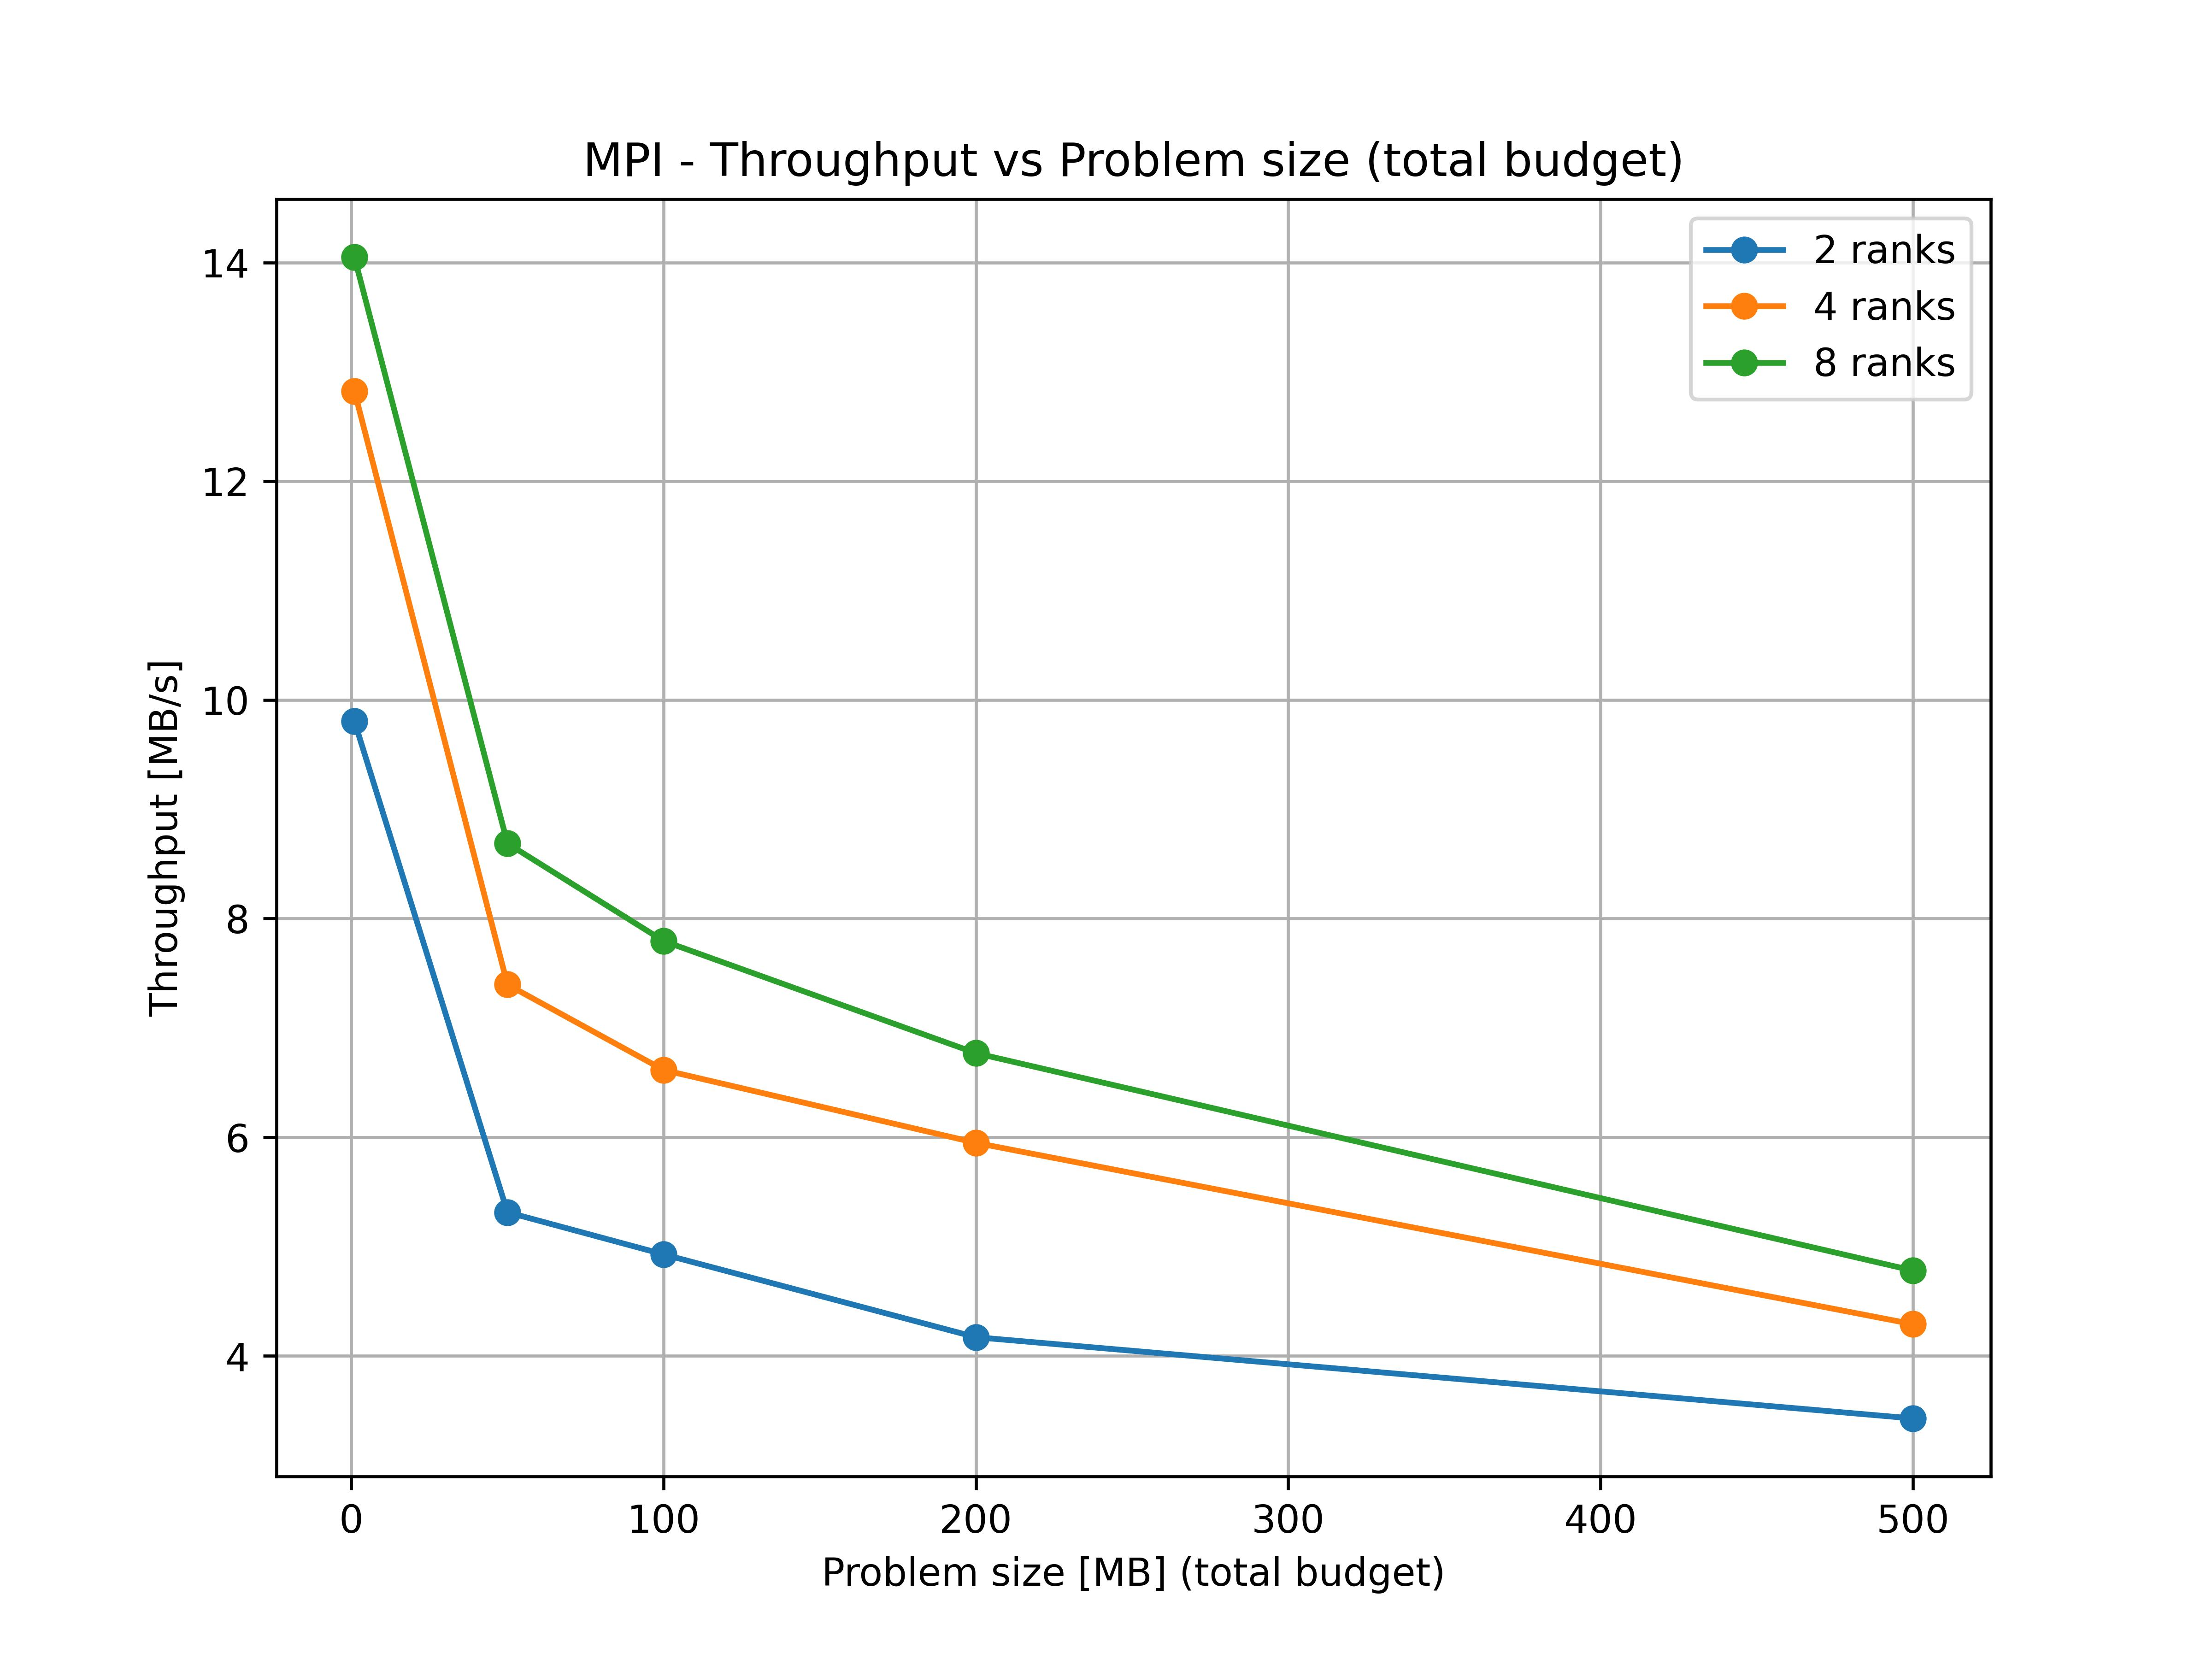
\includegraphics[width=\textwidth]{img/mpi_plots/mpi_throughput.jpg}
					\caption{Throughput MPI}
					\label{fig:mpi_throughput}
				\end{minipage}
			\end{figure}
			
			\begin{figure}[H]
				\centering
				\begin{minipage}[t]{0.49\textwidth}
					\centering
					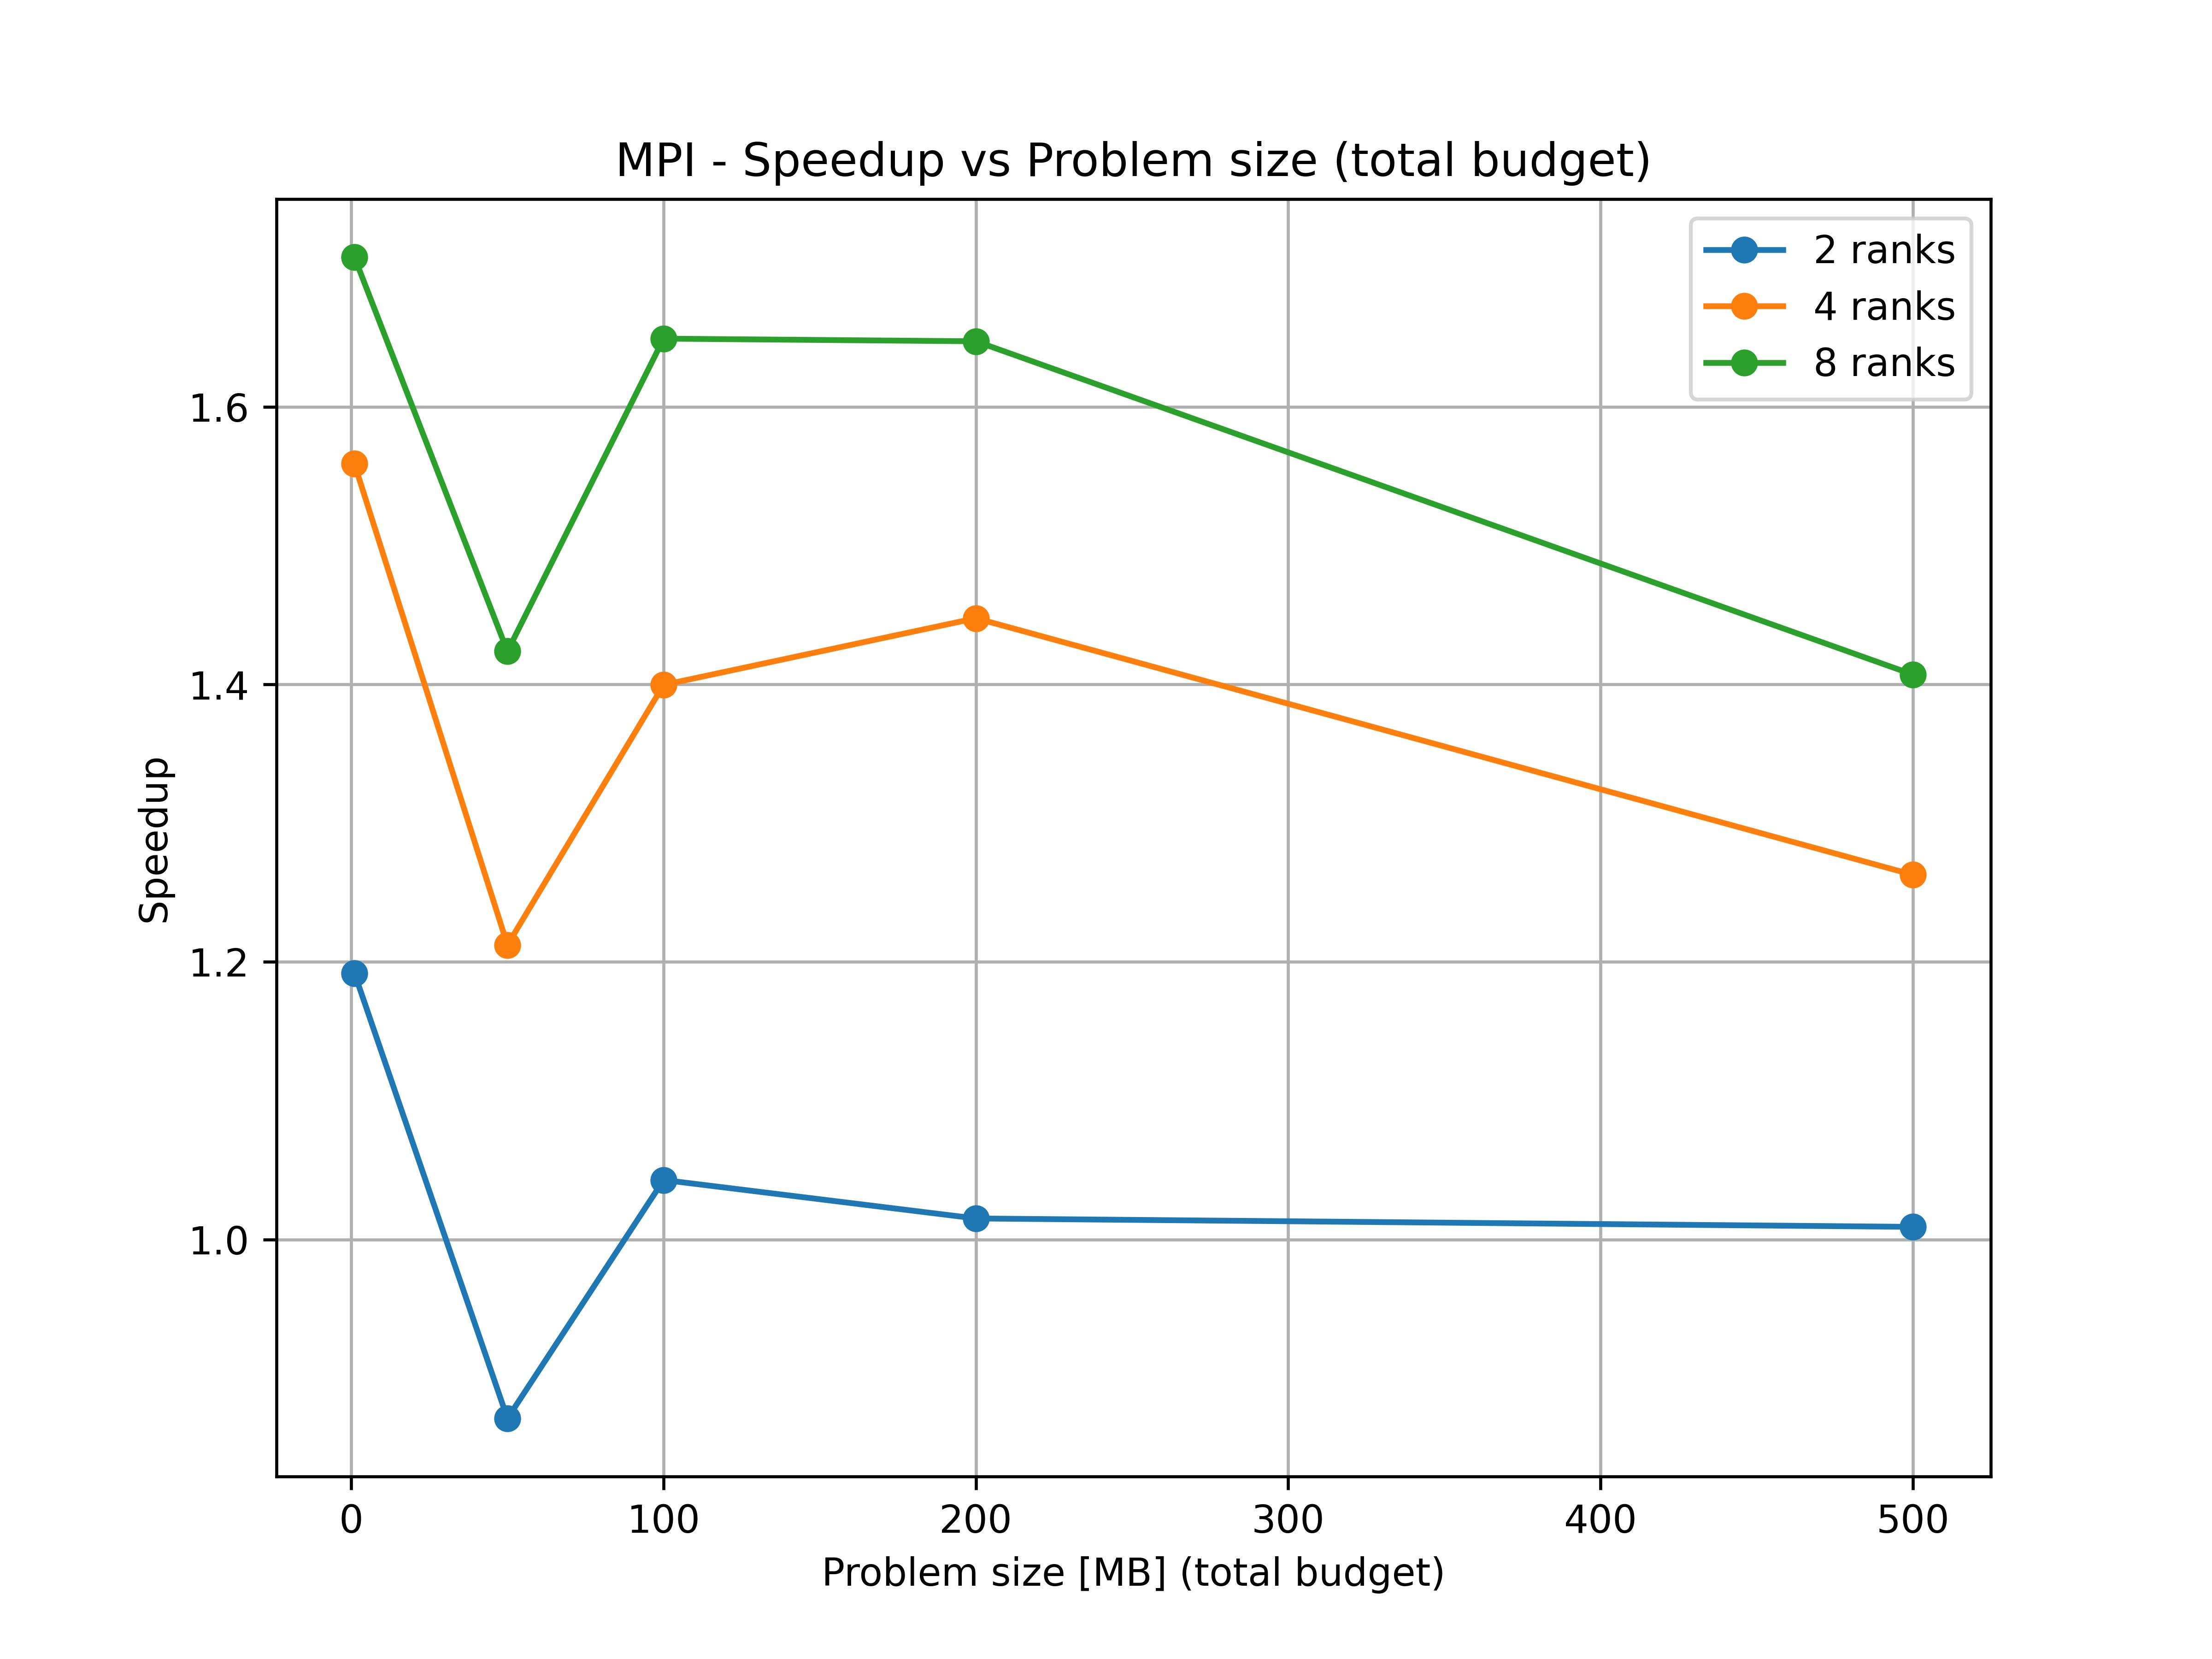
\includegraphics[width=\textwidth]{img/mpi_plots/mpi_speedup.jpg}
					\caption{Speedup MPI}
					\label{fig:mpi_speedup}
				\end{minipage}
				\hfill
				\begin{minipage}[t]{0.49\textwidth}
					\centering
					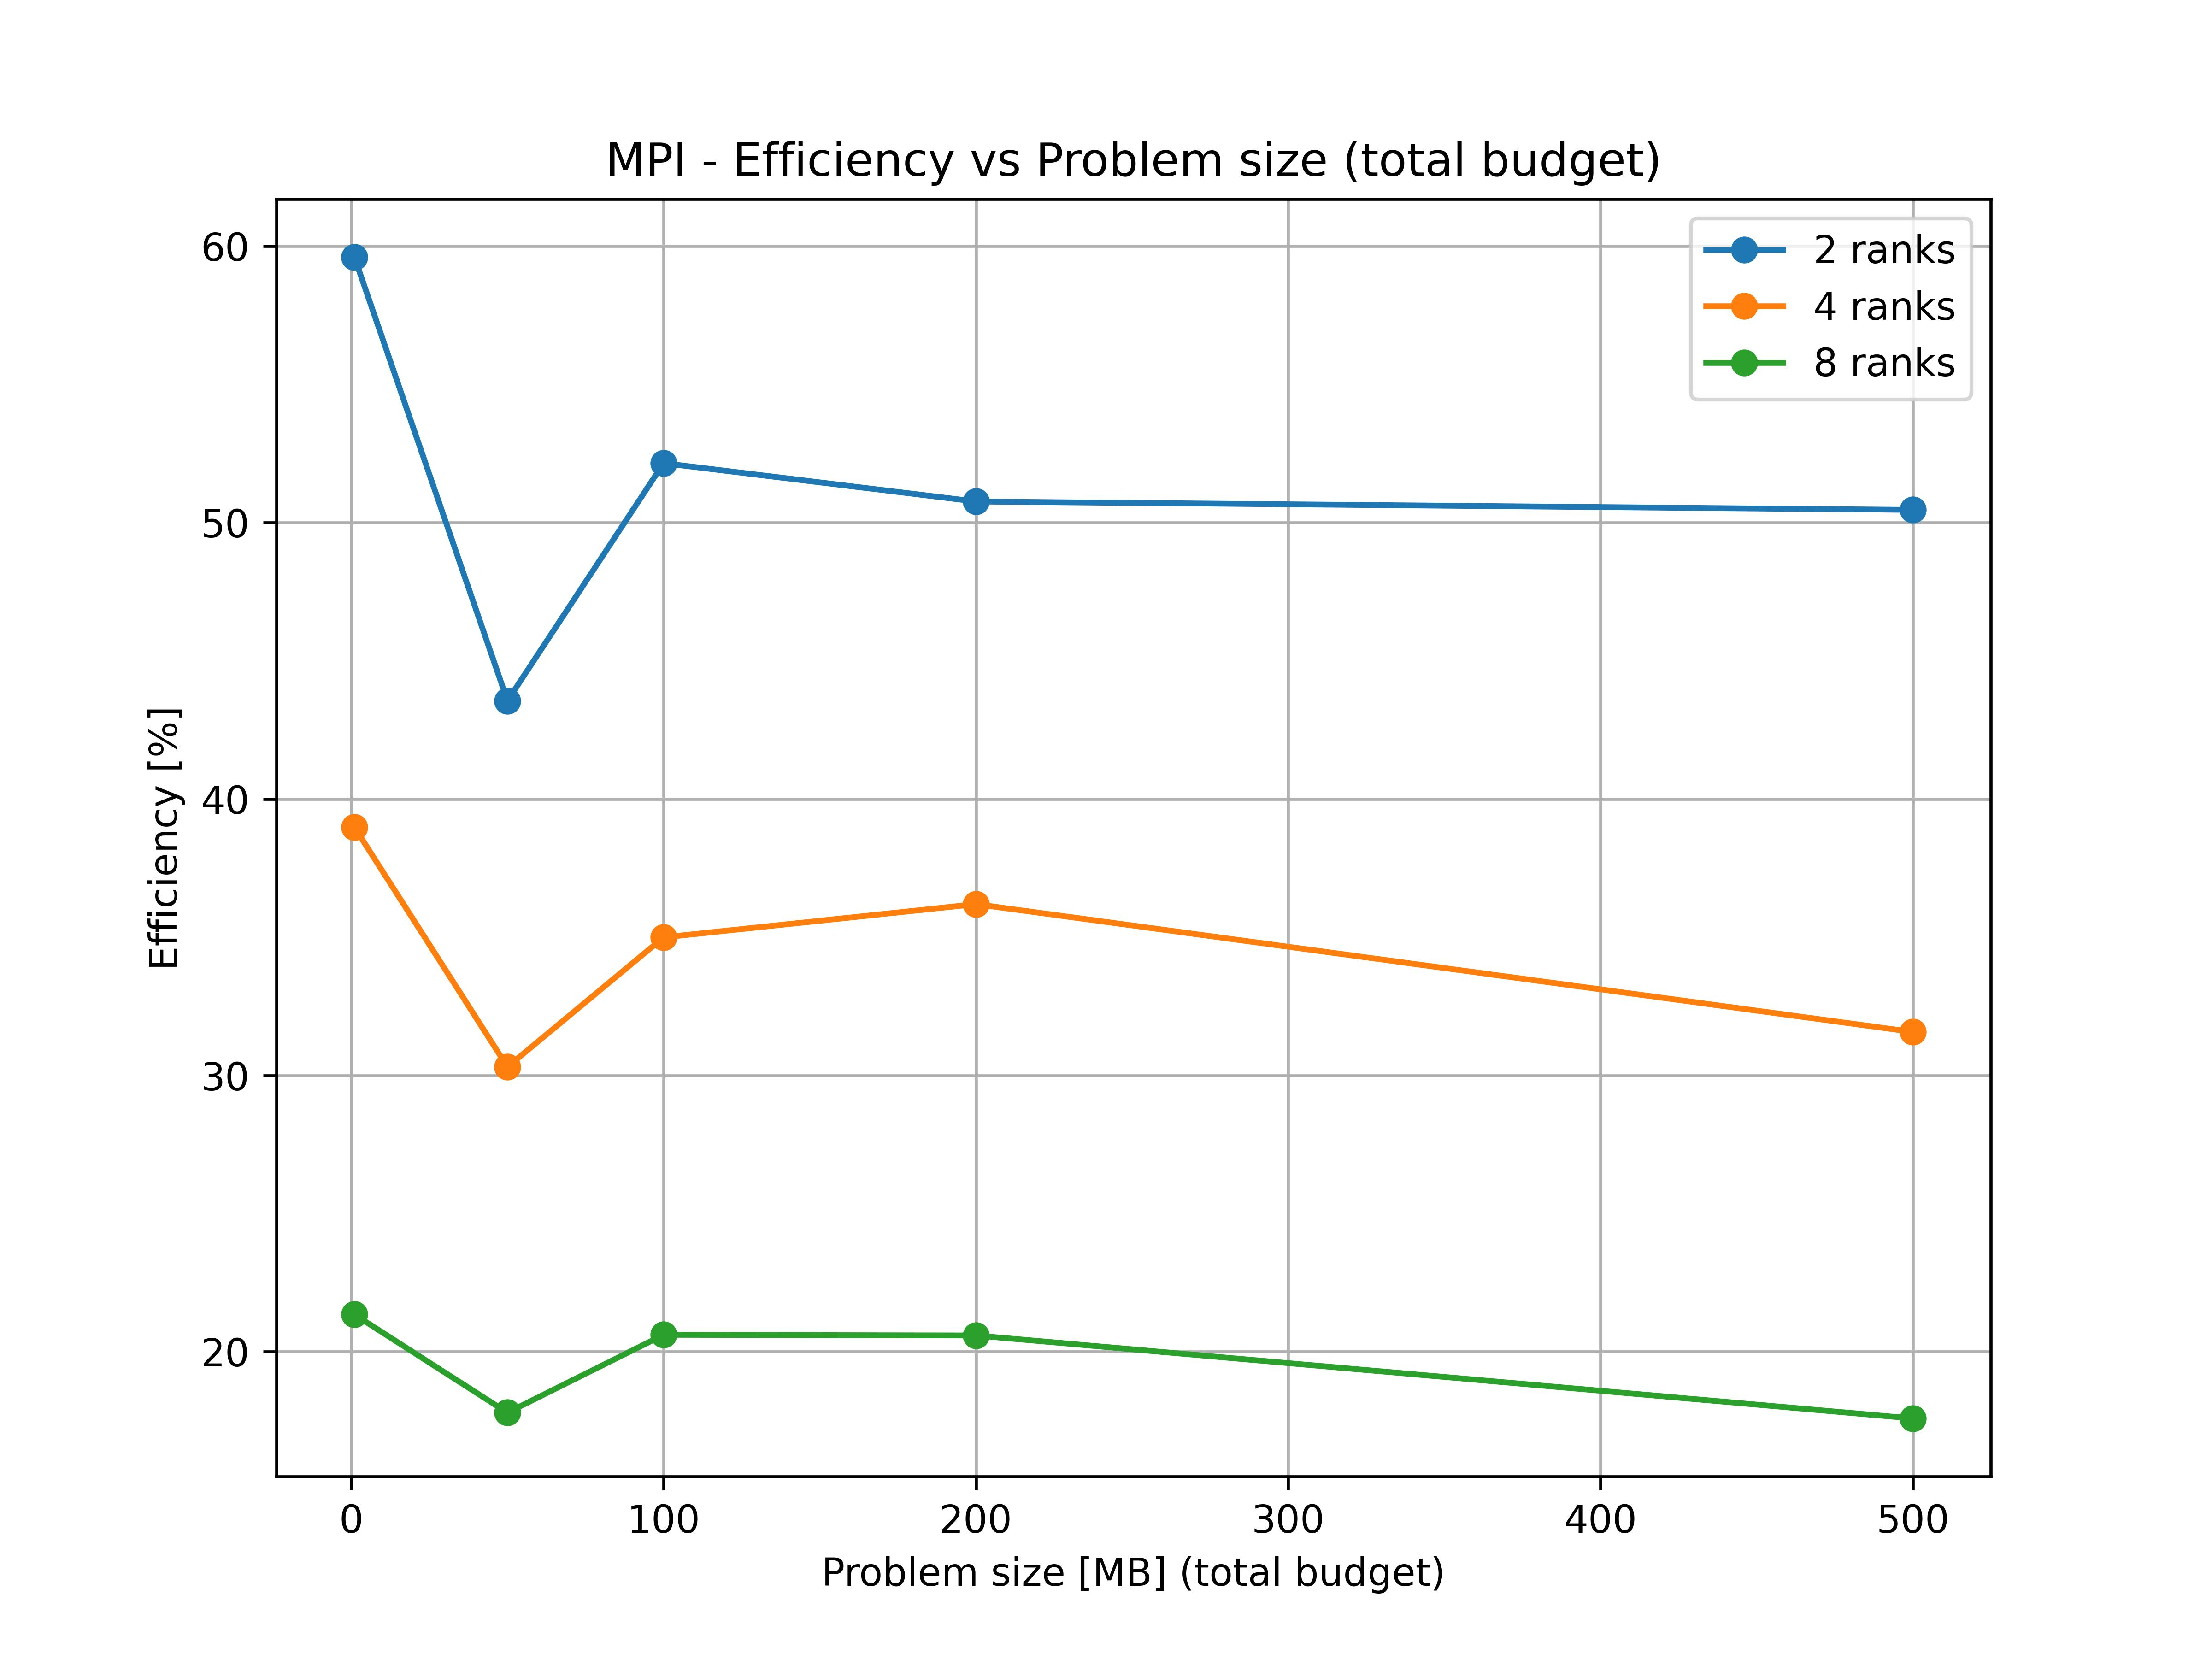
\includegraphics[width=\textwidth]{img/mpi_plots/mpi_efficiency.jpg}
					\caption{Efficiency MPI}
					\label{fig:mpi_efficiency}
				\end{minipage}
			\end{figure}
			
			\subsubsection*{Osservazioni}
				\begin{itemize}
						\item Lo \textbf{speedup} cresce con i ranks, fino a \(\sim 1.65\times\) con 8 processi su 200 MB.
						\item L’\textbf{efficienza} cala: circa \(50\%\) con 2 ranks, \(30\%\) con 4 e sotto il \(20\%\) con 8.
						\item I guadagni sono più marcati su dataset grandi (es.\ 500 MB: da $7.0s$ seq a $5.0s$ con 8 ranks).
						\item Il merge e il calcolo LCP globale restano i principali colli di bottiglia.
				\end{itemize}
		
		\subsection{Profiling della memoria}
			Il profiling con \texttt{valgrind --tool=massif} è stato condotto sul dataset da 500 MB (rank~0).
			I picchi osservati sono:
			
			\begin{itemize}
				\item \textbf{2 ranks}: \(\sim 1.54\) GB, con gran parte della memoria nei vettori \texttt{sa}, \texttt{rk}, \texttt{lcp}.
				\item \textbf{4 ranks}: \(\sim 592\) MB, footprint distribuito più equilibrato.
				\item \textbf{8 ranks}: \(\sim 577\) MB, ma con fasi di merge che portano temporanei picchi fino a \(\sim 405\) MB aggiuntivi.
			\end{itemize}
			
			\begin{figure}[H]
				\centering
				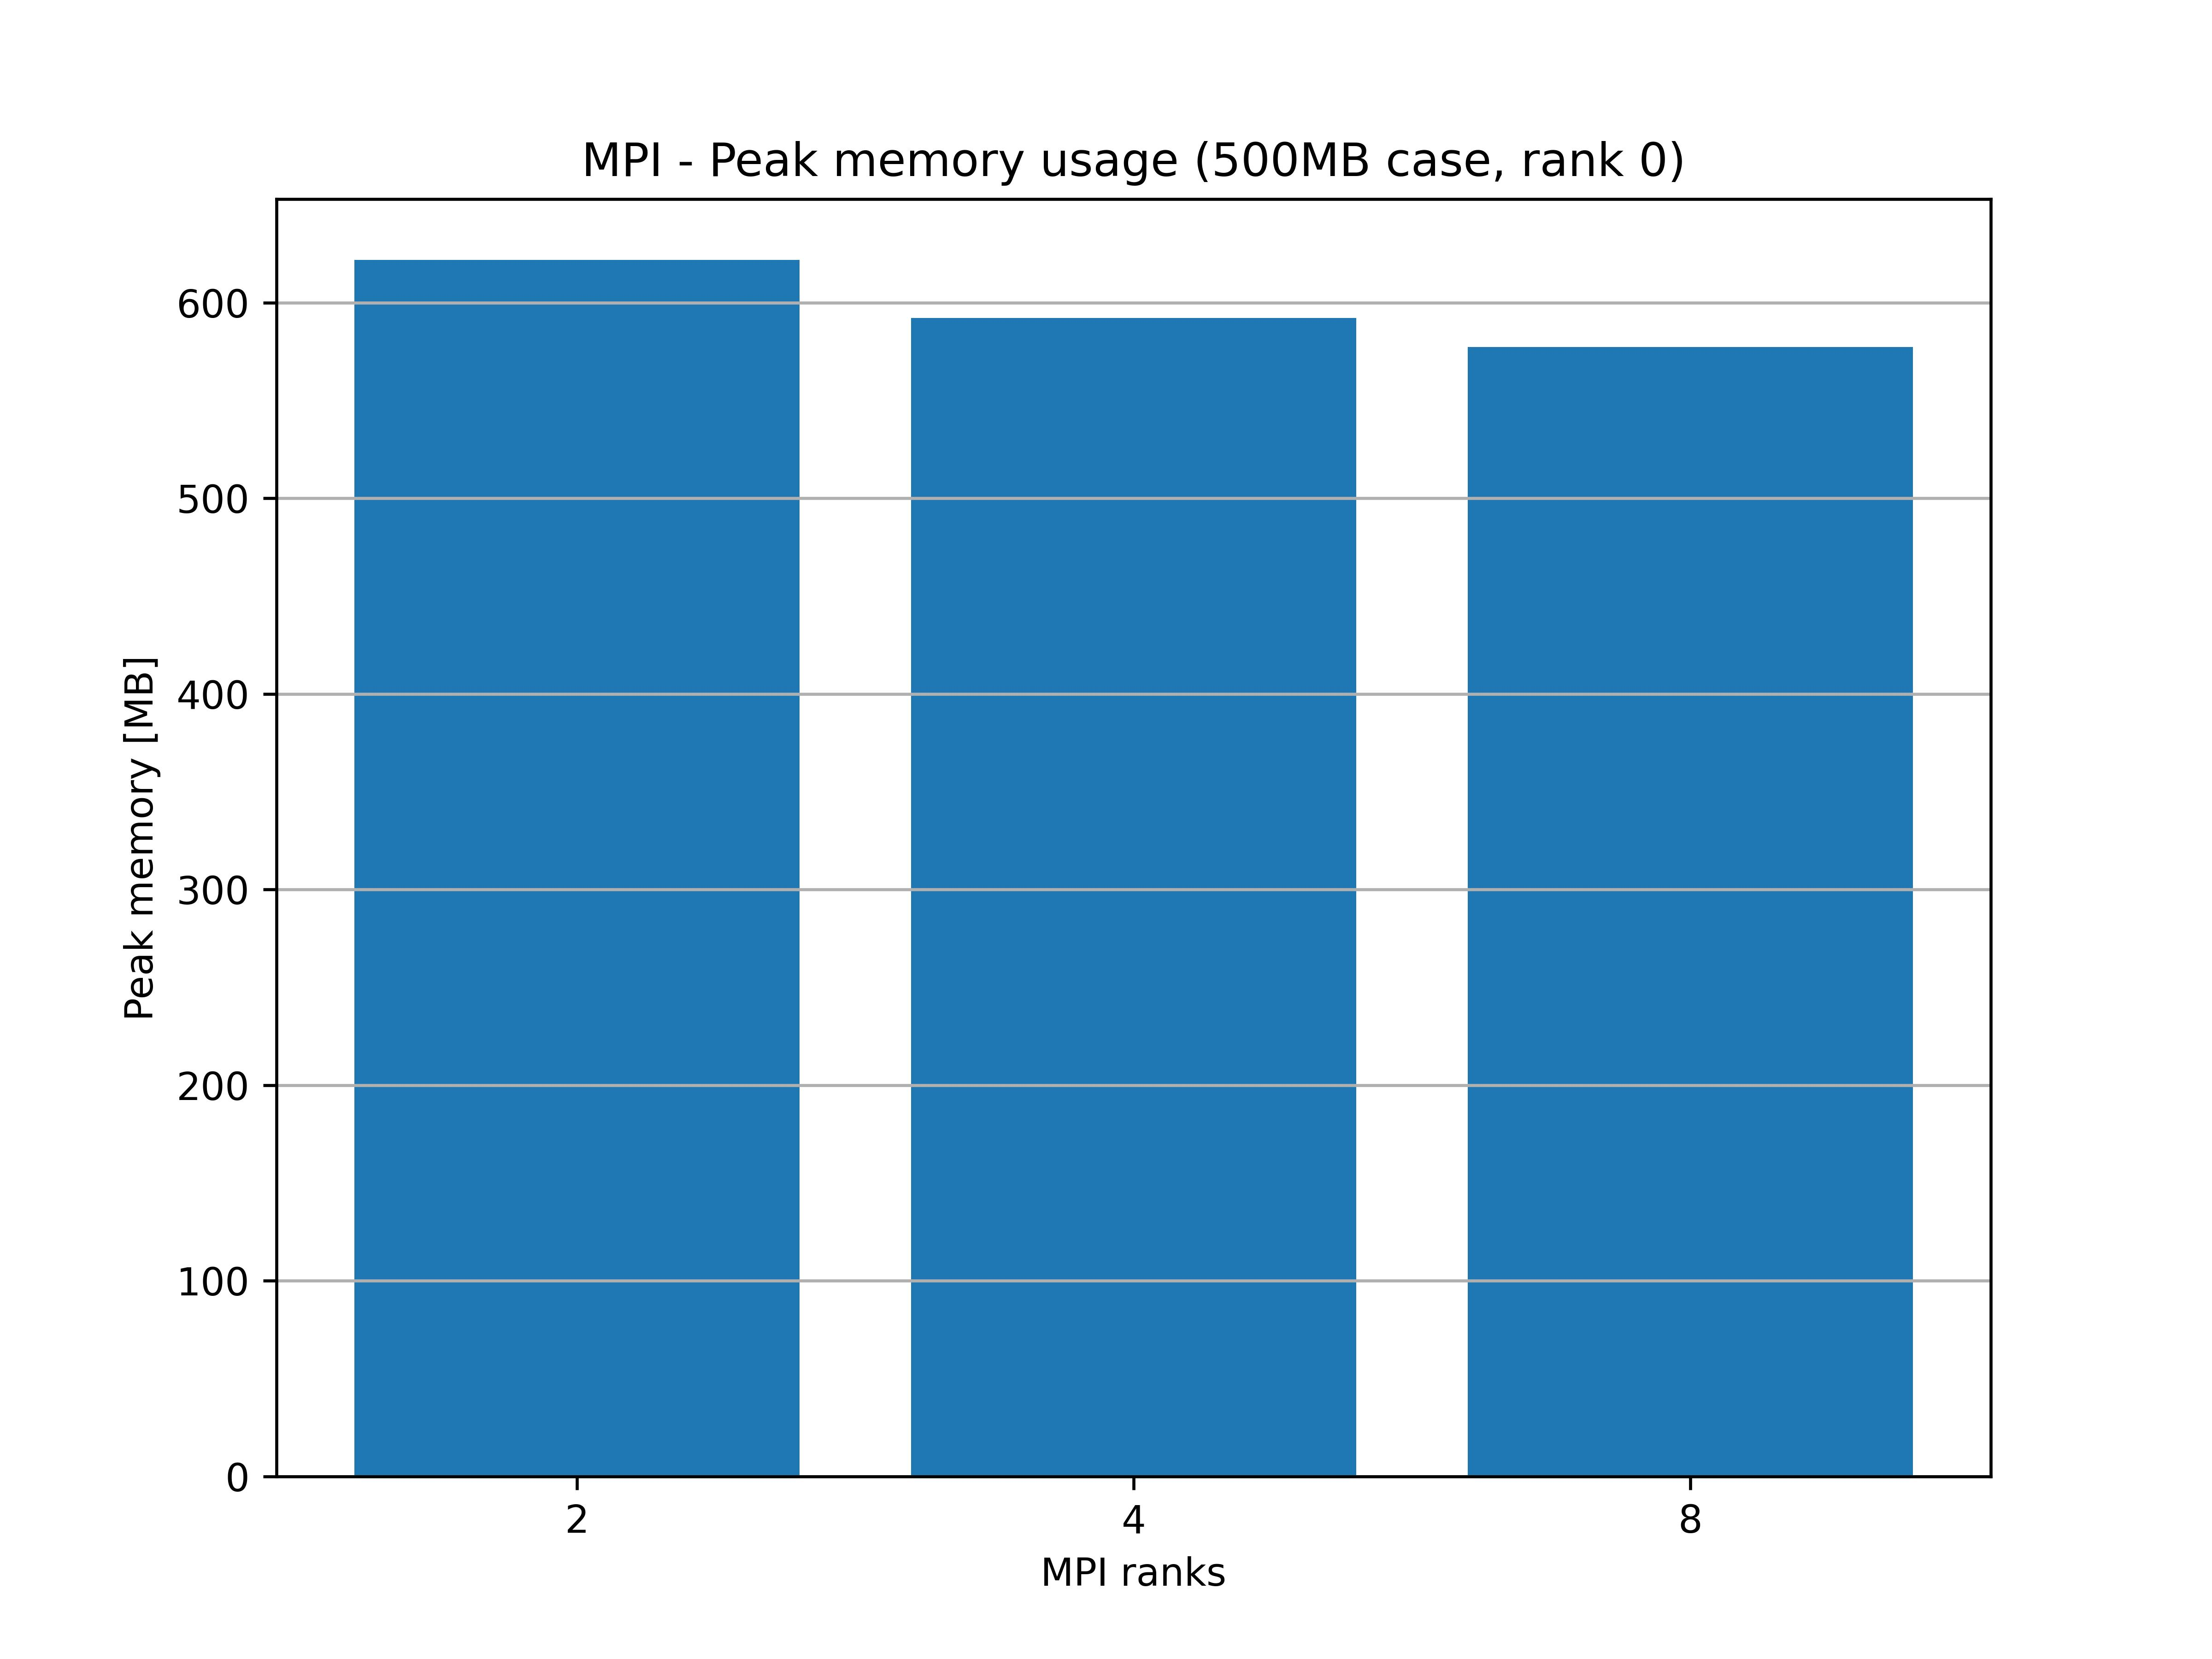
\includegraphics[width=1\linewidth]{img/mpi_plots/mpi_memory.jpg}
				\caption{Memory usage MPI (profiling Massif su rank~0)}
				\label{fig:mpi_mem_usage}
			\end{figure}
			
			\subsubsection*{Conclusione}
				La versione MPI riduce i tempi per input grandi, ma lo scaling è sub-lineare: l’efficienza si abbassa rapidamente oltre i 4 ranks.
				La memoria locale per processo diminuisce all’aumentare dei ranks, ma il rank~0 continua a mostrare picchi elevati durante il merge,
				confermando i limiti intrinseci dell’approccio distribuito.
	
	\section{Versione MPI+OpenMP}
		
		\subsection{Analisi dei tempi}
			Le prestazioni della versione ibrida sono state raccolte con cinque configurazioni ranks $\times$ threads:
			\begin{itemize}
				\item 2 ranks $\times$ 4 threads,
				\item 2 ranks $\times$ 8 threads,
				\item 4 ranks $\times$ 2 threads,
				\item 4 ranks $\times$ 4 threads,
				\item 8 ranks $\times$ 2 threads.
			\end{itemize}
			I risultati medi (10 run) sono riportati nella Tabella~\ref{tab:mpi-omp-summary}.
			
			\begin{table}[H]
				\centering
				\resizebox{\textwidth}{!}{%
					\begin{tabular}{lrrrrr rrrrr rrrrr rrrrr rrrrr}
						\toprule
						& \multicolumn{5}{c}{\textbf{2r$\times$4t}} & \multicolumn{5}{c}{\textbf{2r$\times$8t}} & \multicolumn{5}{c}{\textbf{4r$\times$2t}} & \multicolumn{5}{c}{\textbf{4r$\times$4t}} & \multicolumn{5}{c}{\textbf{8r$\times$2t}} \\
						\cmidrule(lr){2-6}\cmidrule(lr){7-11}\cmidrule(lr){12-16}\cmidrule(lr){17-21}\cmidrule(lr){22-26}
						\textbf{Size} & \textbf{merge} & \textbf{lcp} & \textbf{comm} & \textbf{compute} & \textbf{MB/s} &
						\textbf{merge} & \textbf{lcp} & \textbf{comm} & \textbf{compute} & \textbf{MB/s} &
						\textbf{merge} & \textbf{lcp} & \textbf{comm} & \textbf{compute} & \textbf{MB/s} &
						\textbf{merge} & \textbf{lcp} & \textbf{comm} & \textbf{compute} & \textbf{MB/s} &
						\textbf{merge} & \textbf{lcp} & \textbf{comm} & \textbf{compute} & \textbf{MB/s} \\
						(MB) & (s) & (s) & (s) & (s) & &
						(s) & (s) & (s) & (s) & &
						(s) & (s) & (s) & (s) & &
						(s) & (s) & (s) & (s) & &
						(s) & (s) & (s) & (s) & \\
						\midrule
						1   & 0.00126 & 0.00051 & 0.00002 & 0.00522 & 9.13 & 0.00125 & 0.00050 & 0.00002 & 0.00550 & 8.66 & 0.00190 & 0.00058 & 0.00005 & 0.00411 & 11.59 & 0.00171 & 0.00051 & 0.00003 & 0.00401 & 11.87 & 0.00238 & 0.00060 & 0.00005 & 0.00439 & 11.31 \\
						50  & 0.08514 & 0.05296 & 0.00117 & 0.4419  & 5.39 & 0.08470 & 0.05569 & 0.00135 & 0.4440  & 5.36 & 0.11490 & 0.05455 & 0.00135 & 0.3245 & 7.34 & 0.11659 & 0.05850 & 0.00126 & 0.3330 & 7.17 & 0.14463 & 0.06297 & 0.00156 & 0.2938 & 8.15 \\
						100 & 0.18114 & 0.14643 & 0.00260 & 0.9551  & 4.99 & 0.18087 & 0.15562 & 0.00285 & 0.9755  & 4.88 & 0.24668 & 0.15889 & 0.00297 & 0.7377 & 6.46 & 0.23866 & 0.14889 & 0.00285 & 0.7201 & 6.62 & 0.28422 & 0.15587 & 0.00323 & 0.6203 & 7.70 \\
						200 & 0.44999 & 0.38690 & 0.00415 & 2.2079  & 4.32 & 0.49692 & 0.38877 & 0.00439 & 2.2665  & 4.20 & 0.55881 & 0.38123 & 0.00583 & 1.6593 & 5.75 & 0.52421 & 0.37098 & 0.00579 & 1.6103 & 5.91 & 0.69348 & 0.37936 & 0.00637 & 1.4838 & 6.43 \\
						500 & 2.24016 & 1.15297 & 0.01009 & 7.1236  & 3.34 & 2.05653 & 1.15114 & 0.01035 & 6.8713  & 3.47 & 2.61852 & 1.14213 & 0.01249 & 5.7554 & 4.14 & 2.48589 & 1.11313 & 0.01247 & 5.6125 & 4.25 & 2.83967 & 1.14664 & 0.01525 & 5.1647 & 4.61 \\
						\bottomrule
					\end{tabular}}
				\caption{MPI+OpenMP — Medie (10 run) per size e configurazione.}
				\label{tab:mpi-omp-summary}
			\end{table}
			
			\begin{figure}[H]
				\centering
				\begin{minipage}[t]{0.49\textwidth}
					\centering
					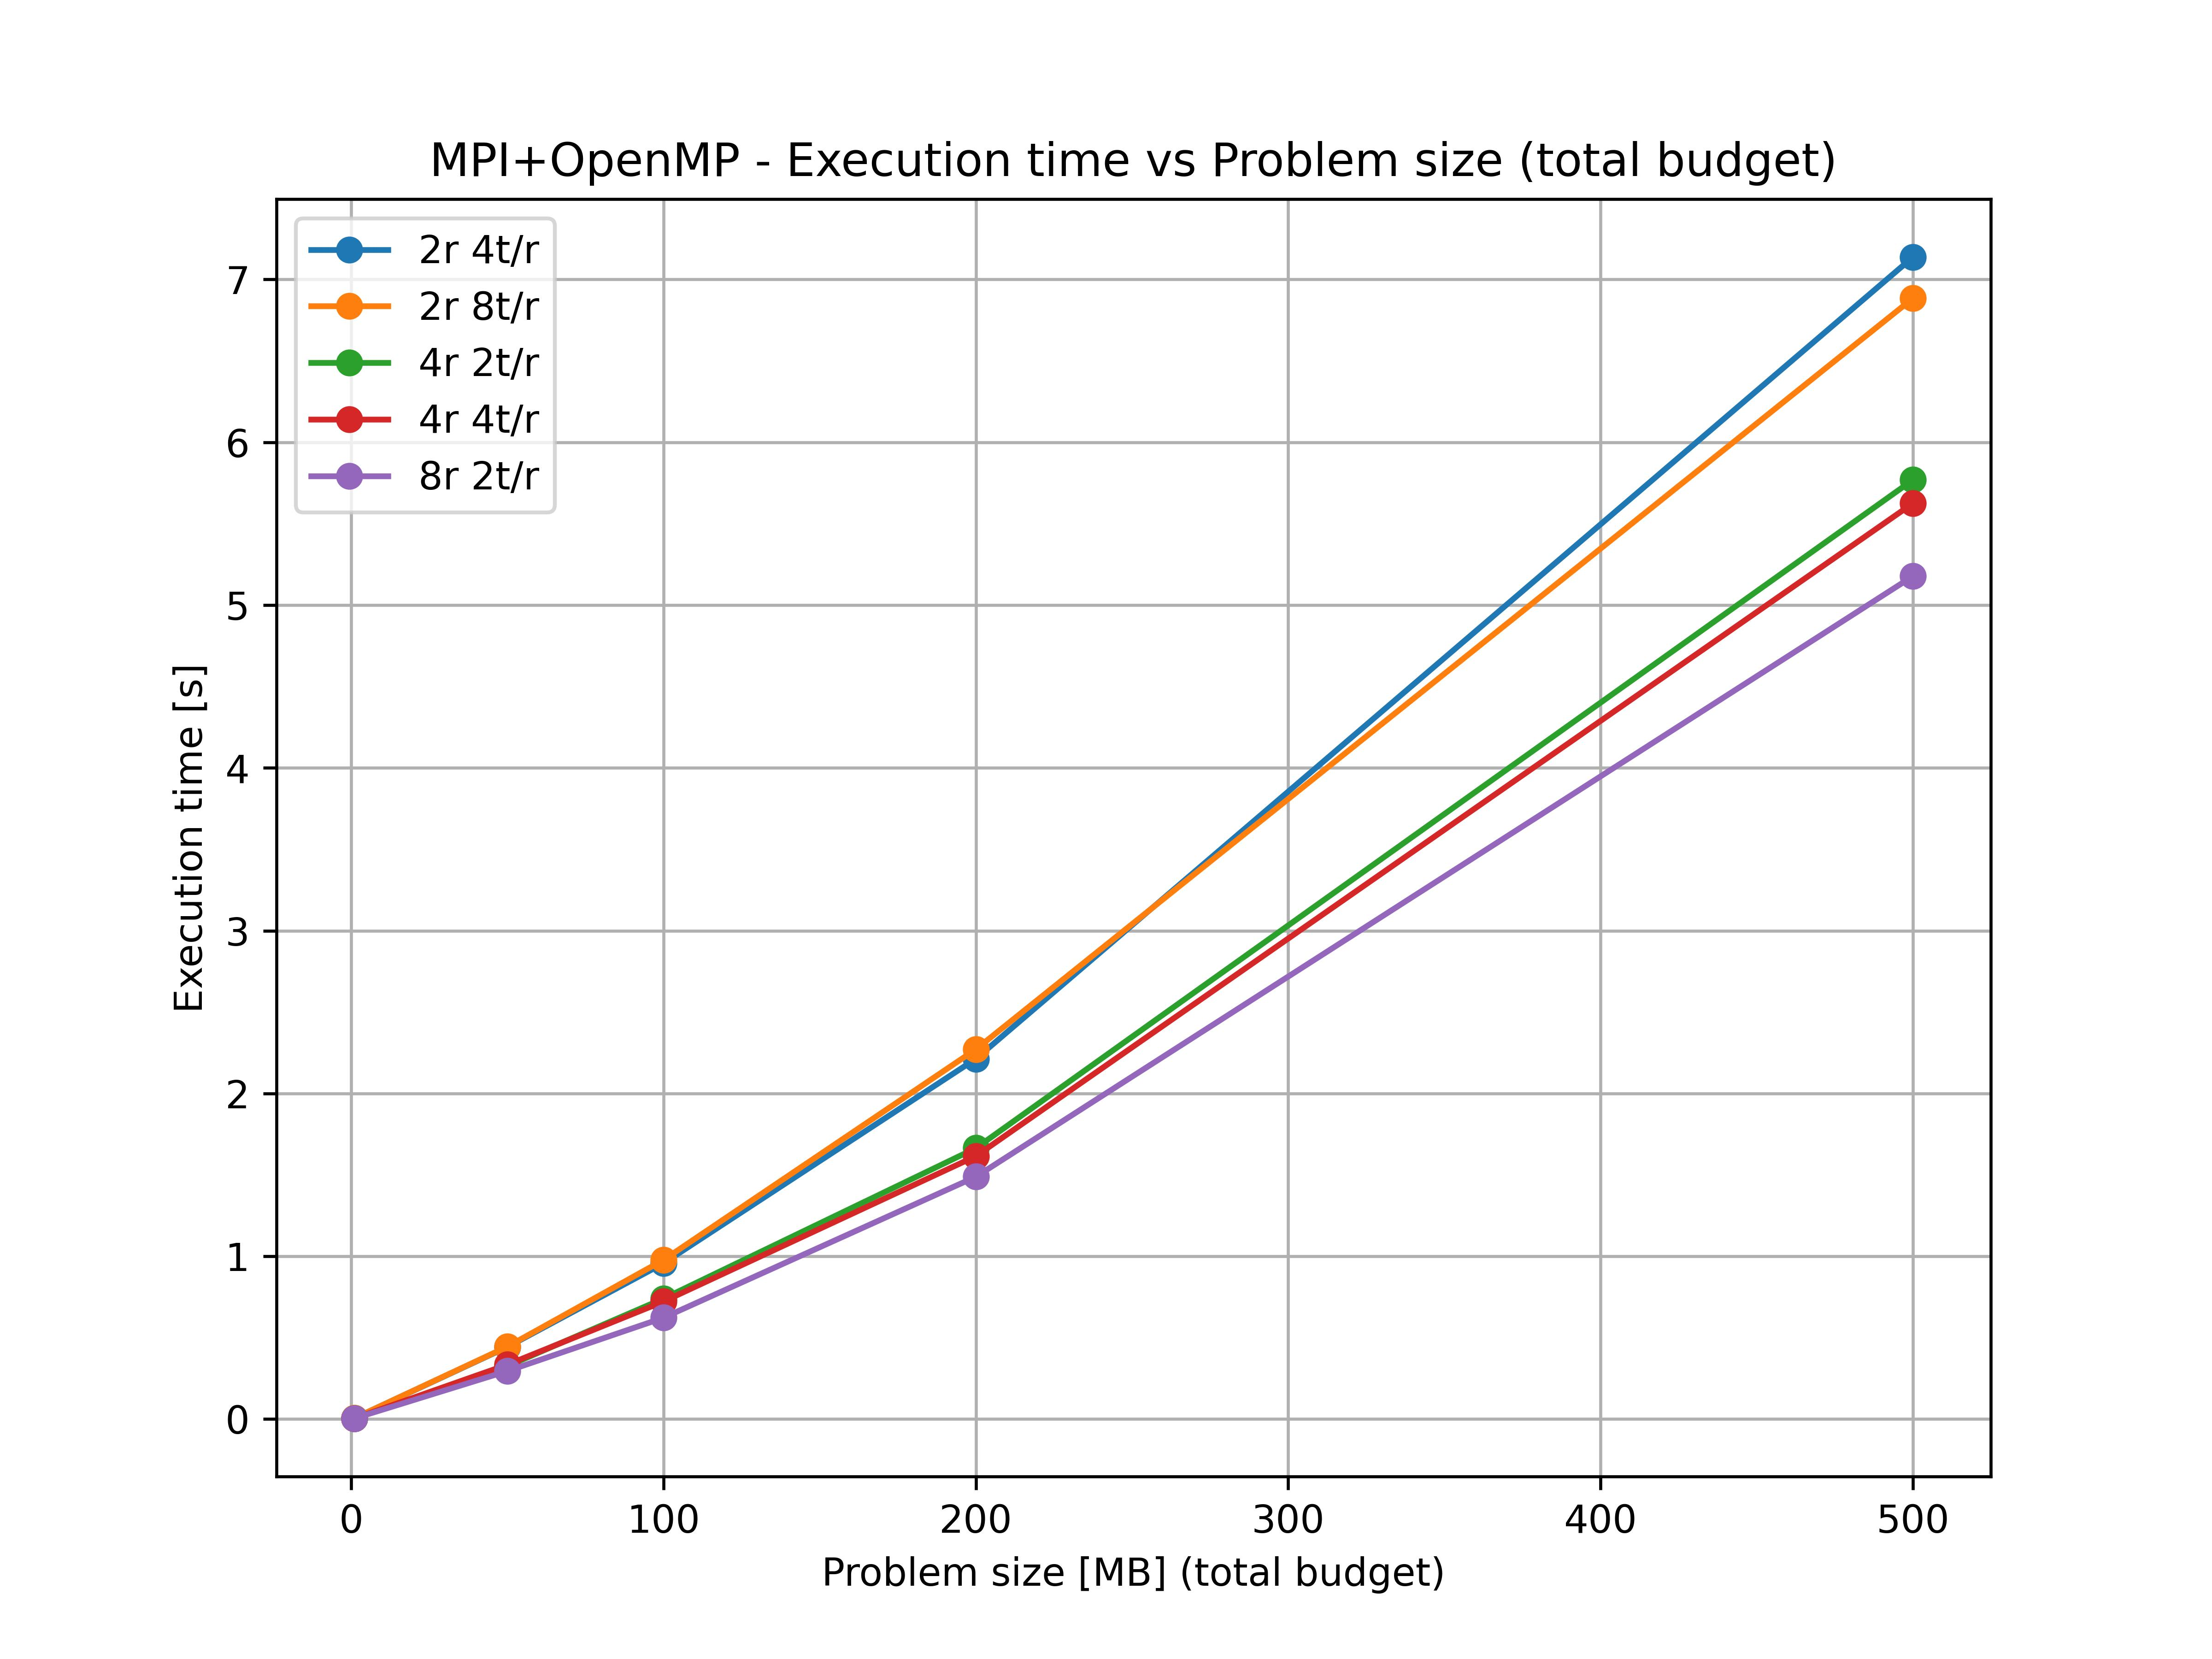
\includegraphics[width=\textwidth]{img/mpi_omp_plots/mpi_omp_times.jpg}
					\caption{Tempi MPI+OMP}
					\label{fig:mpi_omp_times}
				\end{minipage}
				\hfill
				\begin{minipage}[t]{0.49\textwidth}
					\centering
					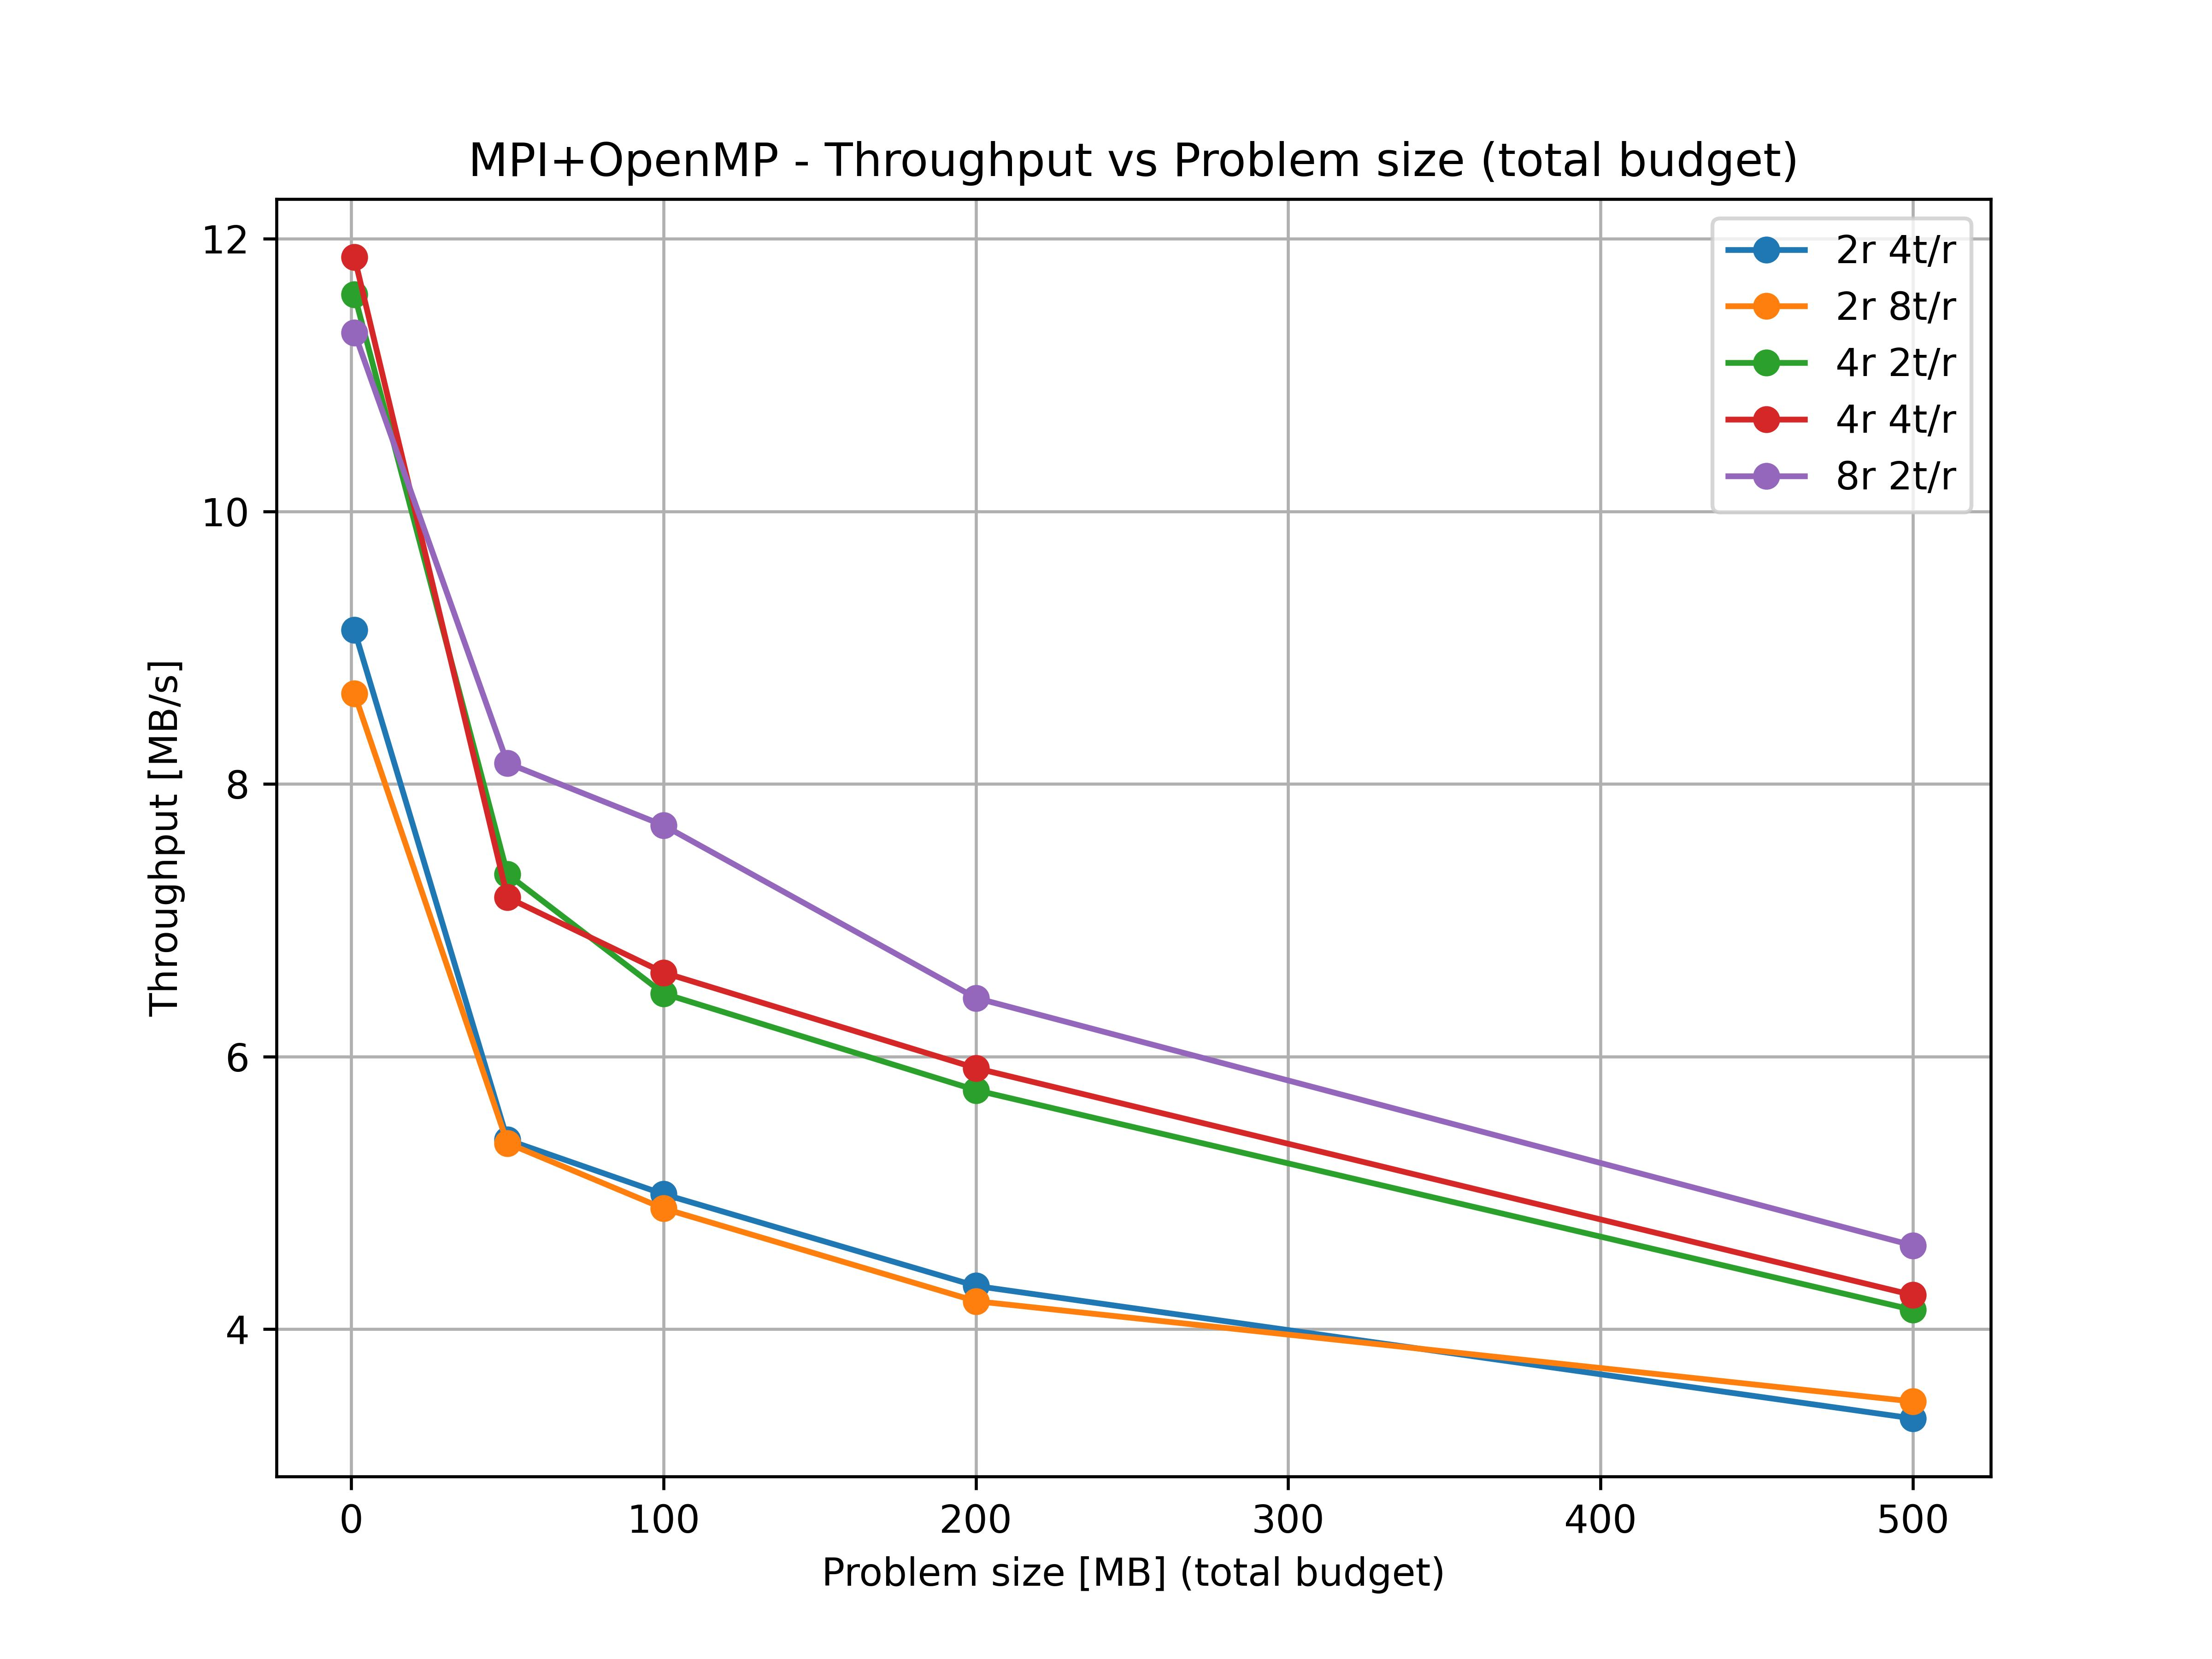
\includegraphics[width=\textwidth]{img/mpi_omp_plots/mpi_omp_throughput.jpg}
					\caption{Throughput MPI+OMP}
					\label{fig:mpi_omp_throughput}
				\end{minipage}
			\end{figure}
			
			\begin{figure}[H]
				\centering
				\begin{minipage}[t]{0.49\textwidth}
					\centering
					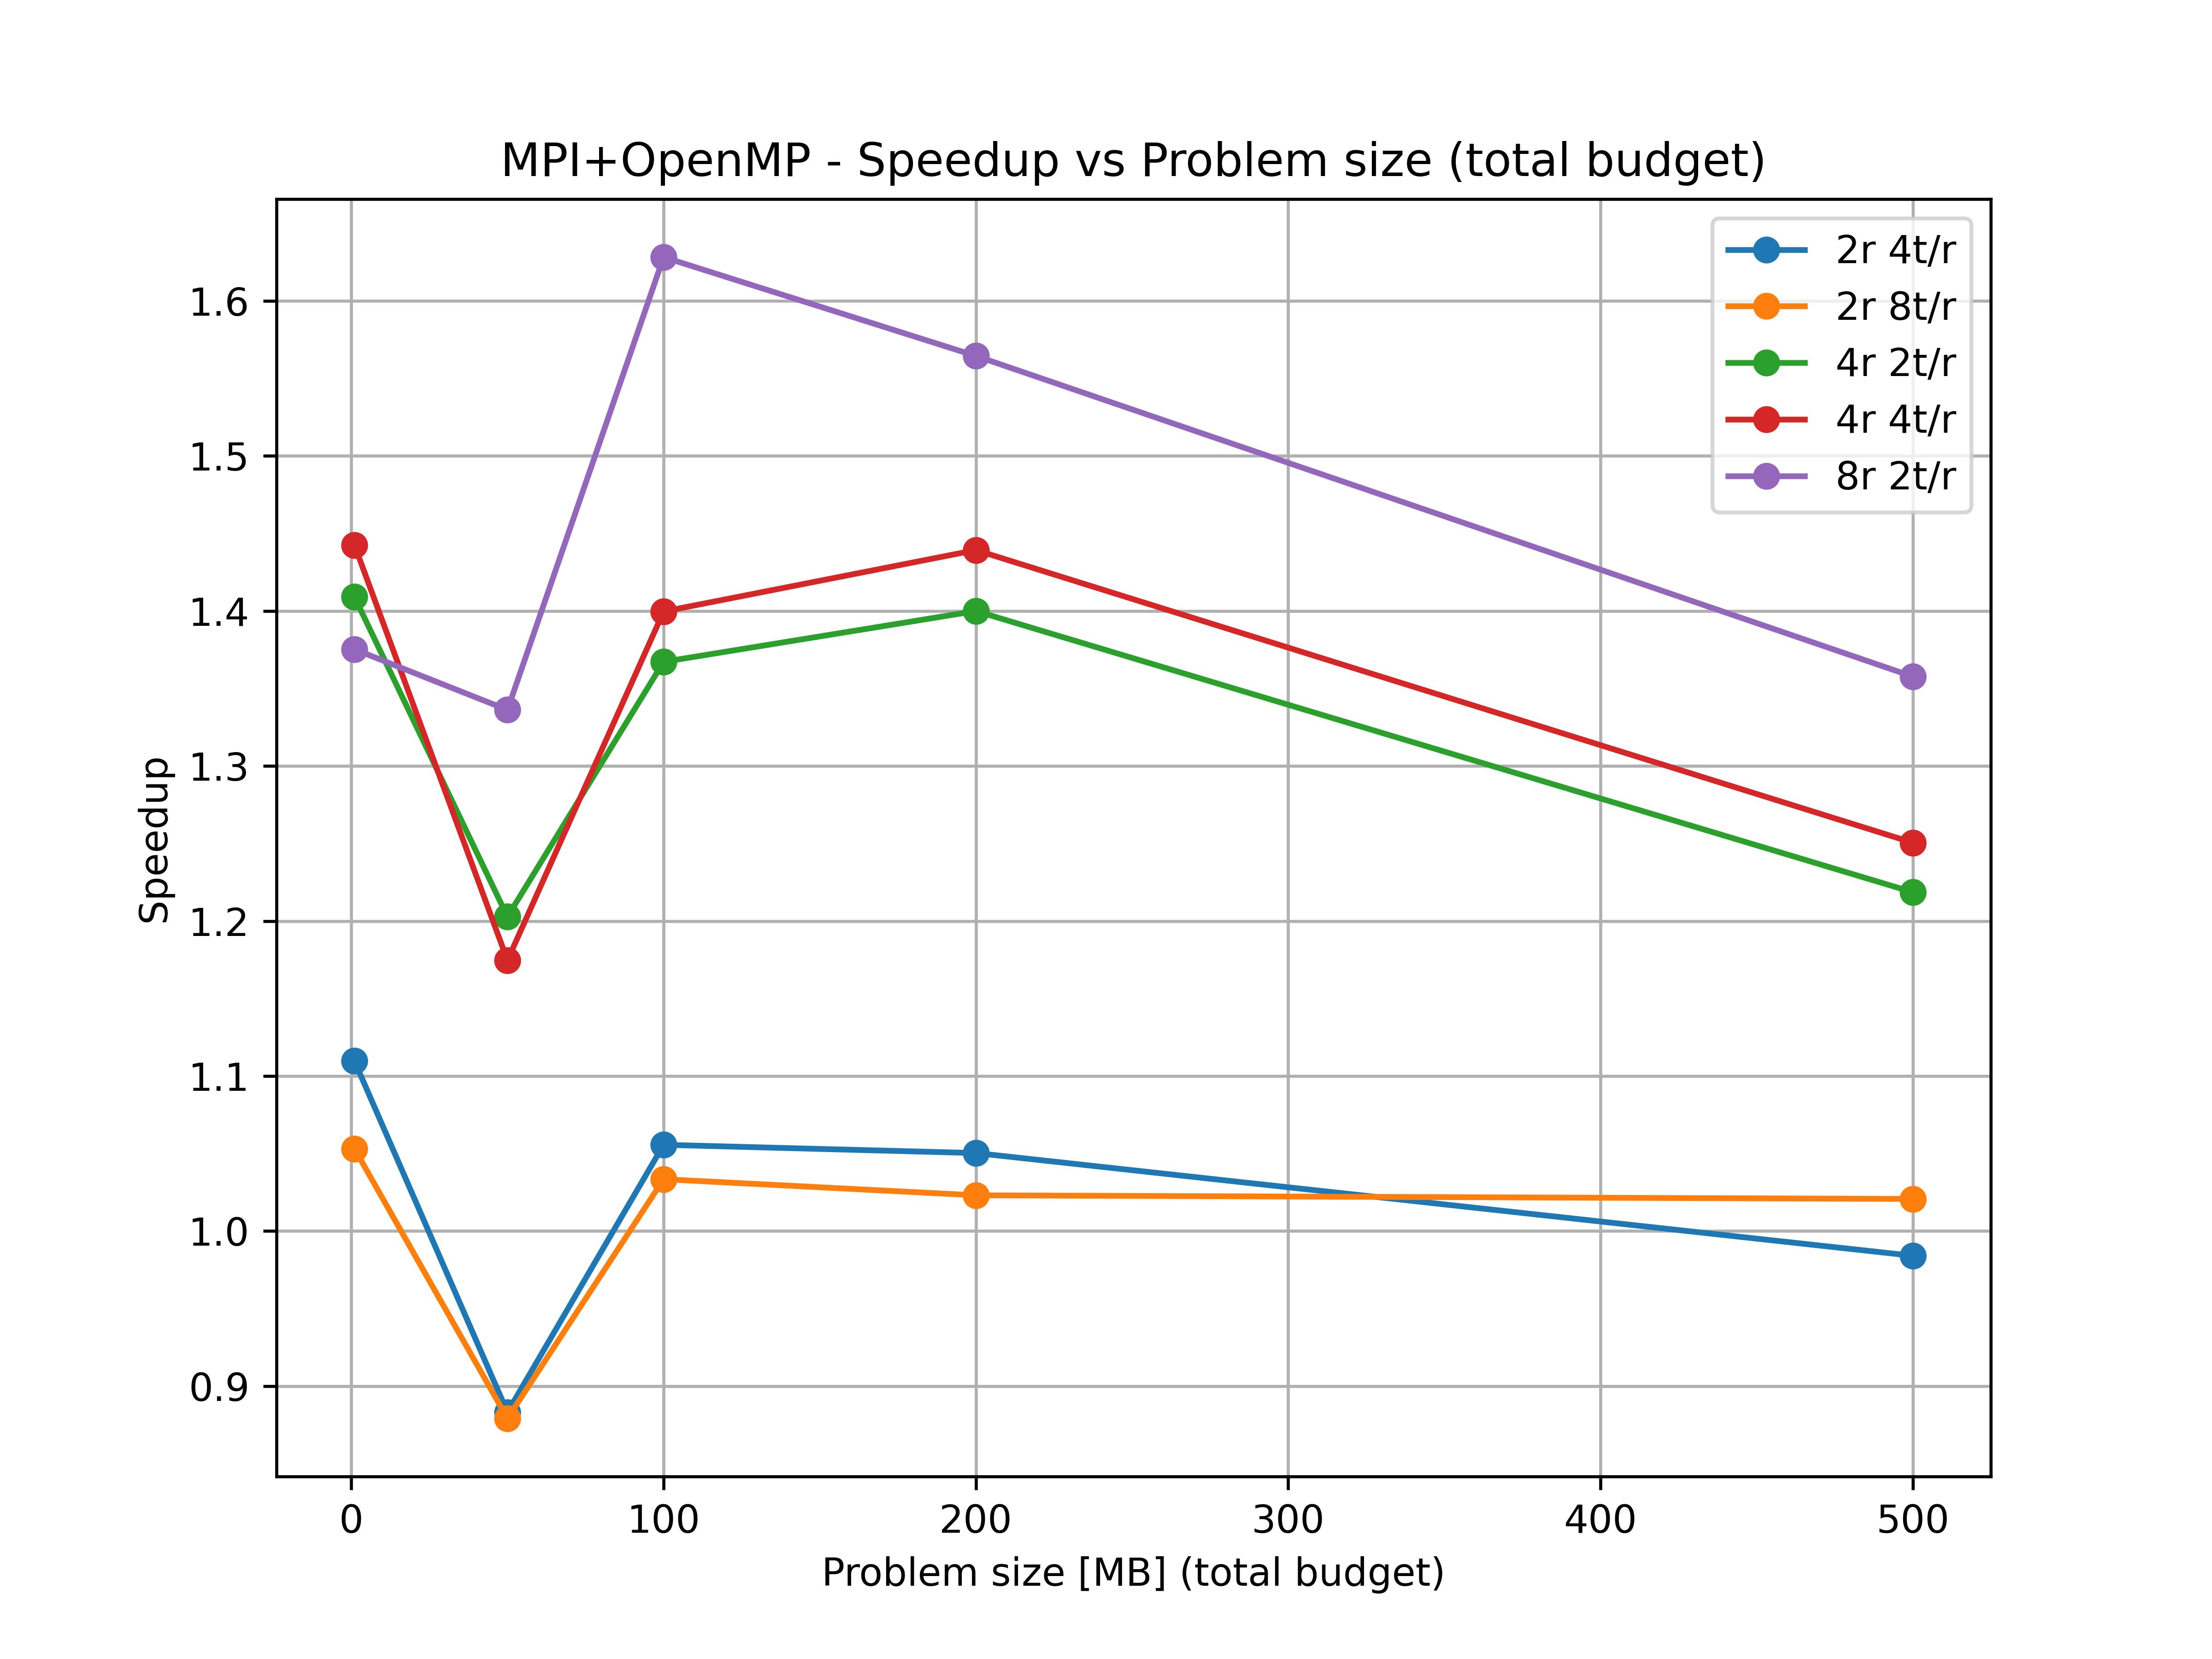
\includegraphics[width=\textwidth]{img/mpi_omp_plots/mpi_omp_speedup.jpg}
					\caption{Speedup MPI+OMP}
					\label{fig:mpi_omp_speedup}
				\end{minipage}
				\hfill
				\begin{minipage}[t]{0.49\textwidth}
					\centering
					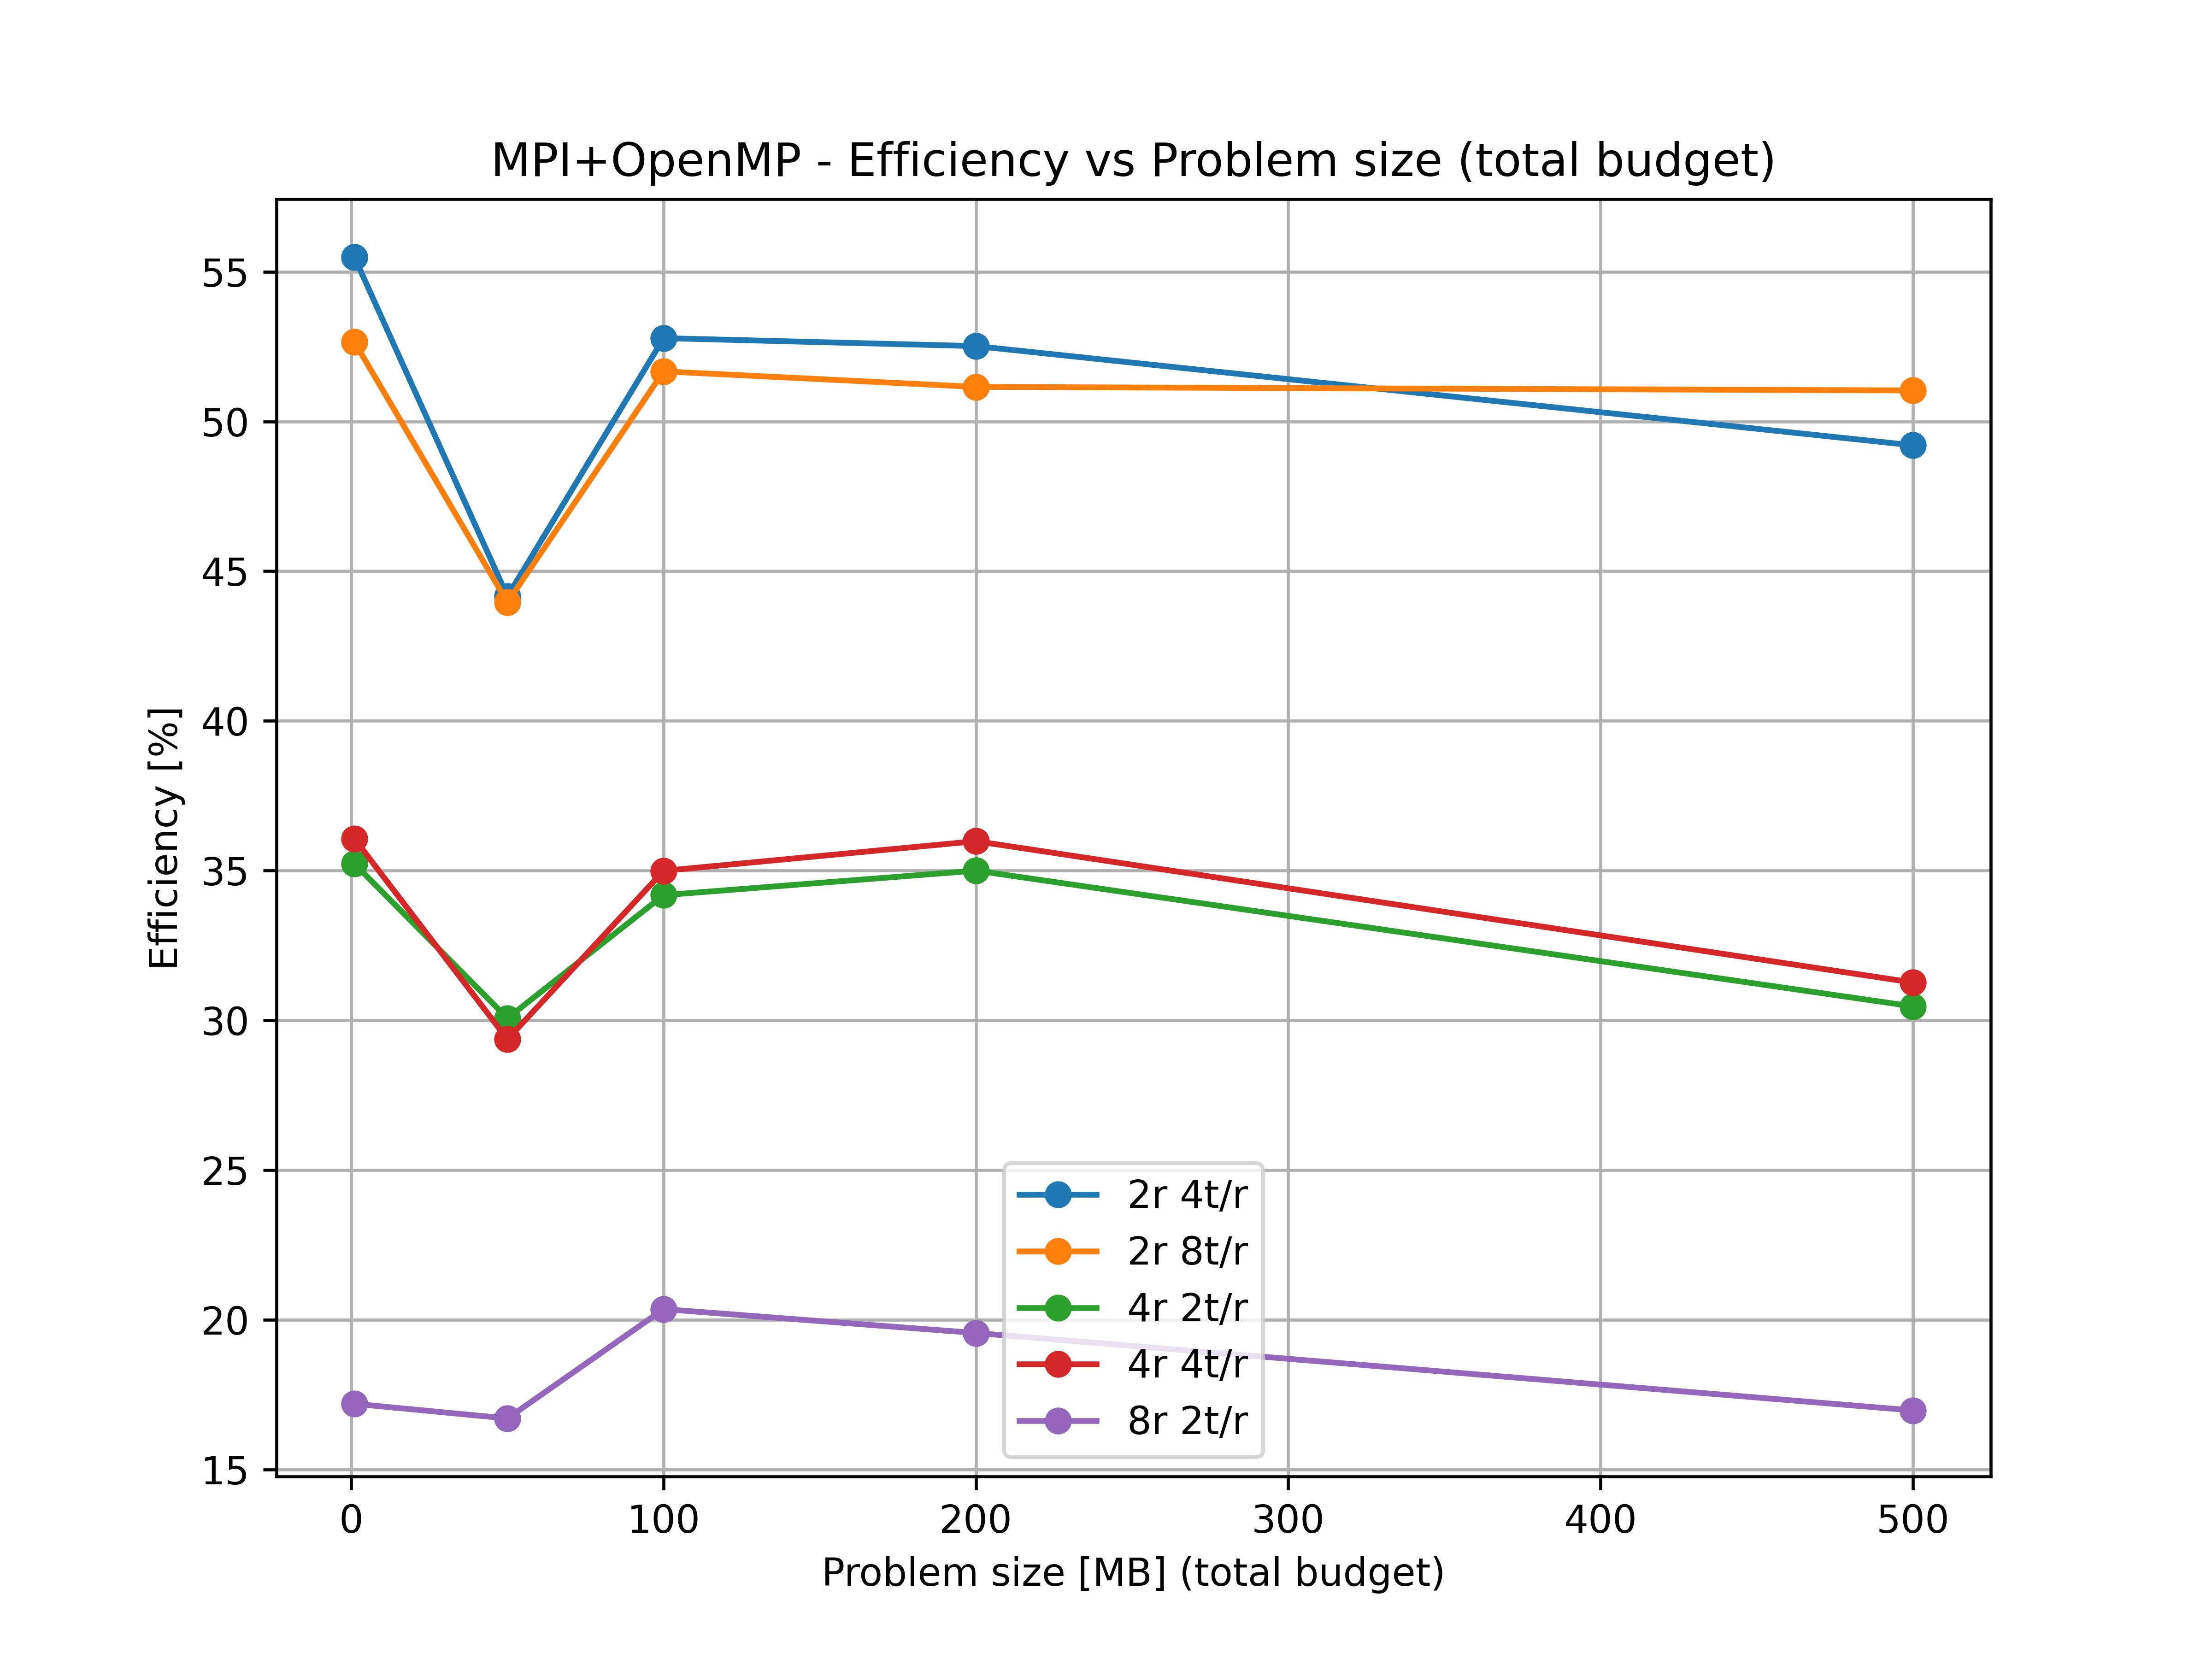
\includegraphics[width=\textwidth]{img/mpi_omp_plots/mpi_omp_efficiency.jpg}
					\caption{Efficiency MPI+OMP}
					\label{fig:mpi_omp_efficiency}
				\end{minipage}
			\end{figure}
			
			\subsubsection*{Osservazioni}
				\begin{itemize}
						\item La configurazione con più ranks e pochi thread (8r$\times$2t) è la più veloce: throughput fino a $\sim$4.6 MB/s e speedup $\sim$1.36$\times$ su 500 MB.
						\item Le configurazioni bilanciate (4r$\times$2t, 4r$\times$4t) ottengono tempi intermedi con efficienze $\sim$30–36\%.
						\item Le configurazioni a 2 ranks (sia 4t che 8t) hanno efficienza più alta (oltre 50\%), ma tempi assoluti peggiori.
						\item L’efficienza cala sistematicamente con l’aumento dei ranks, per via del merge distribuito e della comunicazione.
				\end{itemize}
		
		\subsection{Profiling della memoria}
			Il profiling della memoria è stato condotto su input da 500 MB, strumentando il \emph{rank~0}.
			
			\subsubsection{2 ranks}
				\begin{itemize}
						\item \textbf{2r$\times$4t}: picco $\sim$ \textbf{492 MB}.
						\item \textbf{2r$\times$8t}: picco $\sim$ \textbf{490 MB}.
						\item In entrambi i casi il consumo è simile: array SA/rank da $\sim$100–150 MB ciascuno, buffer \texttt{text} $\sim$50 MB, strutture temporanee di merge.
				\end{itemize}
			
			\subsubsection{4 ranks}
				\begin{itemize}
						\item \textbf{4r$\times$2t}: picco $\sim$ \textbf{460 MB}.
						\item \textbf{4r$\times$4t}: picco $\sim$ \textbf{459 MB}.
						\item La riduzione rispetto a 2 ranks è limitata, poiché rank~0 deve gestire fasi di merge più pesanti.
				\end{itemize}
			
			\subsubsection{8 ranks}
				\begin{itemize}
						\item \textbf{8r$\times$2t}: picco $\sim$ \textbf{333 MB}.
						\item È la configurazione più leggera: la dimensione locale $n_\text{loc}$ ridotta porta a un consumo sensibilmente inferiore.
				\end{itemize}
				
				\begin{figure}[H]
						\centering
						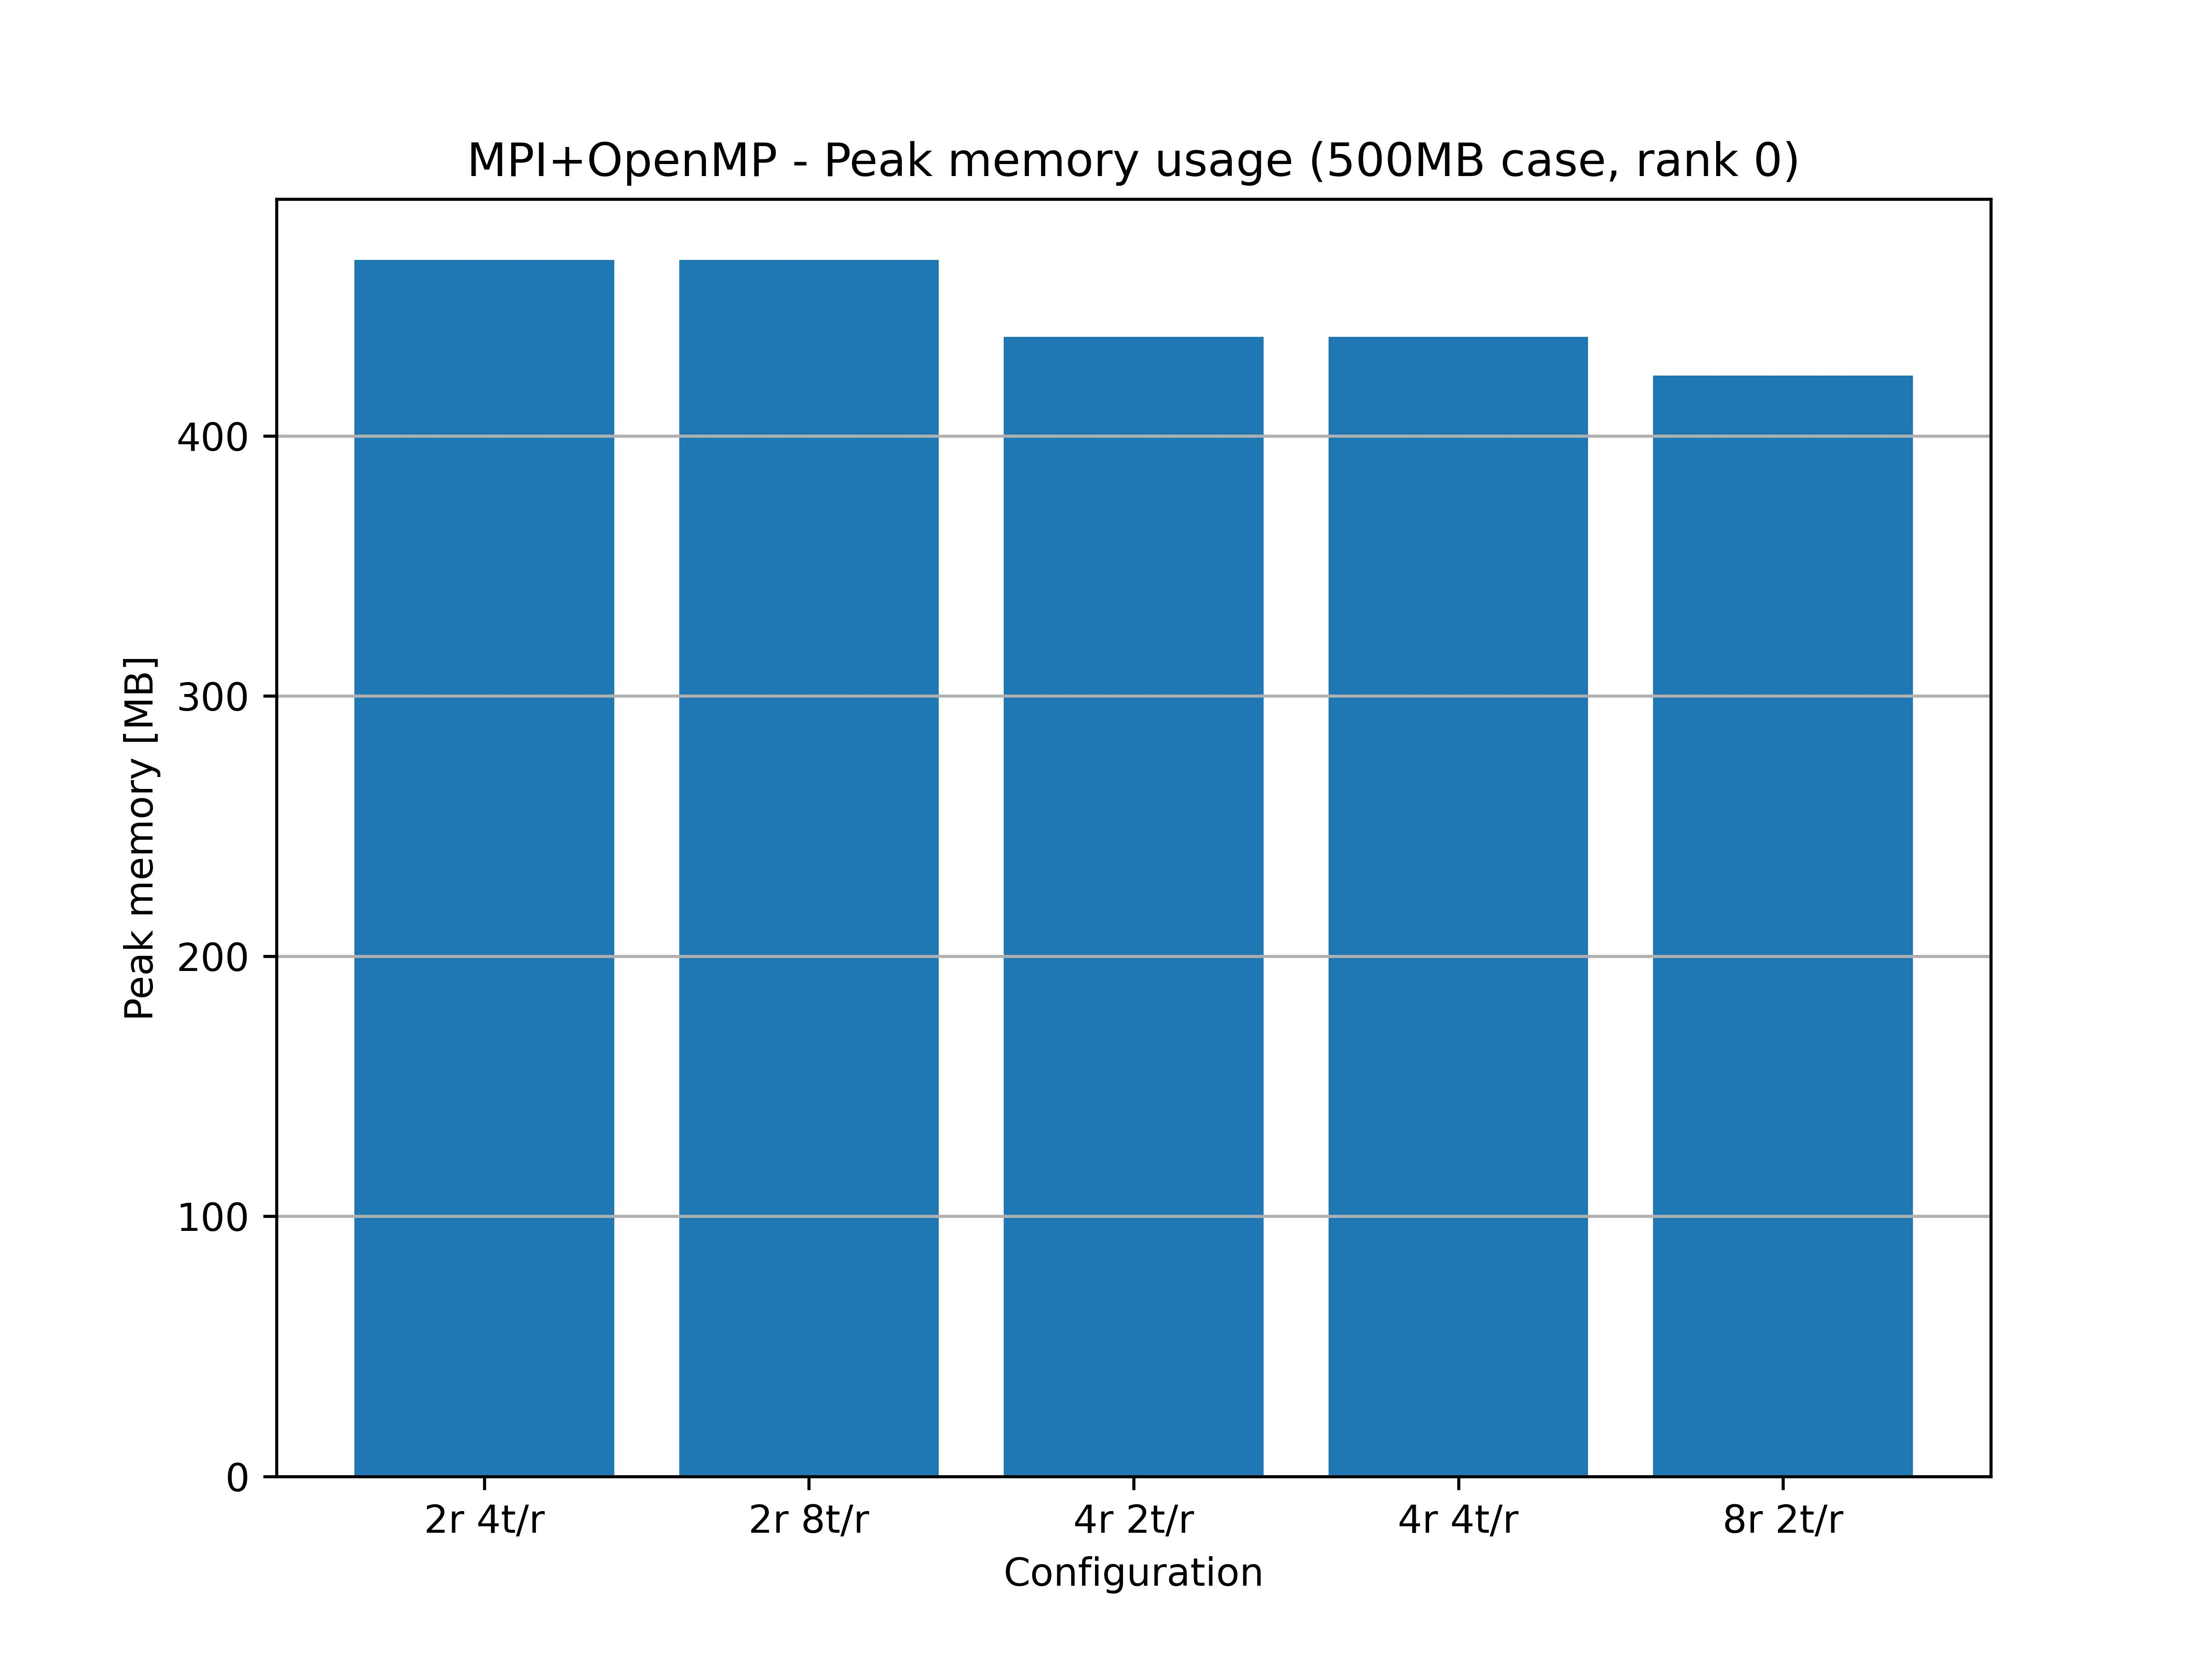
\includegraphics[width=1\linewidth]{img/mpi_omp_plots/mpi_omp_memory.jpg}
						\caption{Memory usage MPI+OMP (rank~0, input 500 MB).}
						\label{fig:mpi_omp_mem_usage}
				\end{figure}
			
			\subsubsection*{Conclusione}
				La memoria scala quasi linearmente con $n_\text{loc}$, scendendo da circa 490 MB (2 ranks) a 333 MB (8 ranks).
				OpenMP non influisce sul footprint, in quanto i thread condividono le strutture dati.
	
	\section{Versione CUDA (single-stream)}
		
		\subsection{Analisi dei tempi}
			I test CUDA (stream singolo) sono stati eseguiti su input da \(\{1,50,100,200,500\}\) MB, 10 run ciascuno, tramite lo script \texttt{cuda\_measure.sh}, che ha prodotto i file \texttt{cuda\_stats.csv} (run grezzi) e \texttt{cuda\_summary.csv} (medie per size).
			La Tabella~\ref{tab:cuda-times} riporta le medie per fase e le metriche aggregate.
			
			\begin{table}[H]
				\centering
				\resizebox{\textwidth}{!}{%
					\begin{tabular}{r r r r r r r r r r r}
						\toprule
						\textbf{Size} & \textbf{Alloc} & \textbf{H2D} & \textbf{Kernel} & \textbf{LCP(CPU)} & \textbf{D2H} &
						\textbf{Compute} & \textbf{Total} & \textbf{Comm} & \textbf{MB/s} & \textbf{Speedup / Eff.} \\
						\textbf{(MB)} & \textbf{(s)} & \textbf{(s)} & \textbf{(s)} & \textbf{(s)} & \textbf{(s)} &
						\textbf{pure (s)} & \textbf{compute (s)} & \textbf{(s)} &  & \textbf{(\(\times\) / \%)} \\
						\midrule
						1   & 0.1153 & 0.00002 & 0.0040 & 0.00045 & 0.00016 & 0.00447 & 0.1198 & 0.00018 & 10.67 & 1.30 / 129.7 \\
						50  & 0.1098 & 0.00030 & 0.0741 & 0.0584  & 0.00572 & 0.1325  & 0.2422 & 0.00602 & 17.99 & 2.95 / 294.9 \\
						100 & 0.1014 & 0.00066 & 0.1468 & 0.1545  & 0.01111 & 0.3013  & 0.4027 & 0.01176 & 15.81 & 3.34 / 334.4 \\
						200 & 0.1001 & 0.00142 & 0.3132 & 0.3746  & 0.02208 & 0.6878  & 0.7879 & 0.02350 & 13.85 & 3.37 / 337.0 \\
						500 & 0.1013 & 0.00366 & 0.8466 & 1.1234  & 0.05524 & 1.9700  & 2.0712 & 0.05891 & 12.09 & 3.56 / 355.7 \\
						\bottomrule
					\end{tabular}}
				\caption{CUDA single-stream — Medie (10 run) per dimensione: tempi per fase, throughput e speedup/efficienza.}
				\label{tab:cuda-times}
			\end{table}
			
			\begin{figure}[H]
				\centering
				\begin{minipage}[t]{0.49\textwidth}
					\centering
					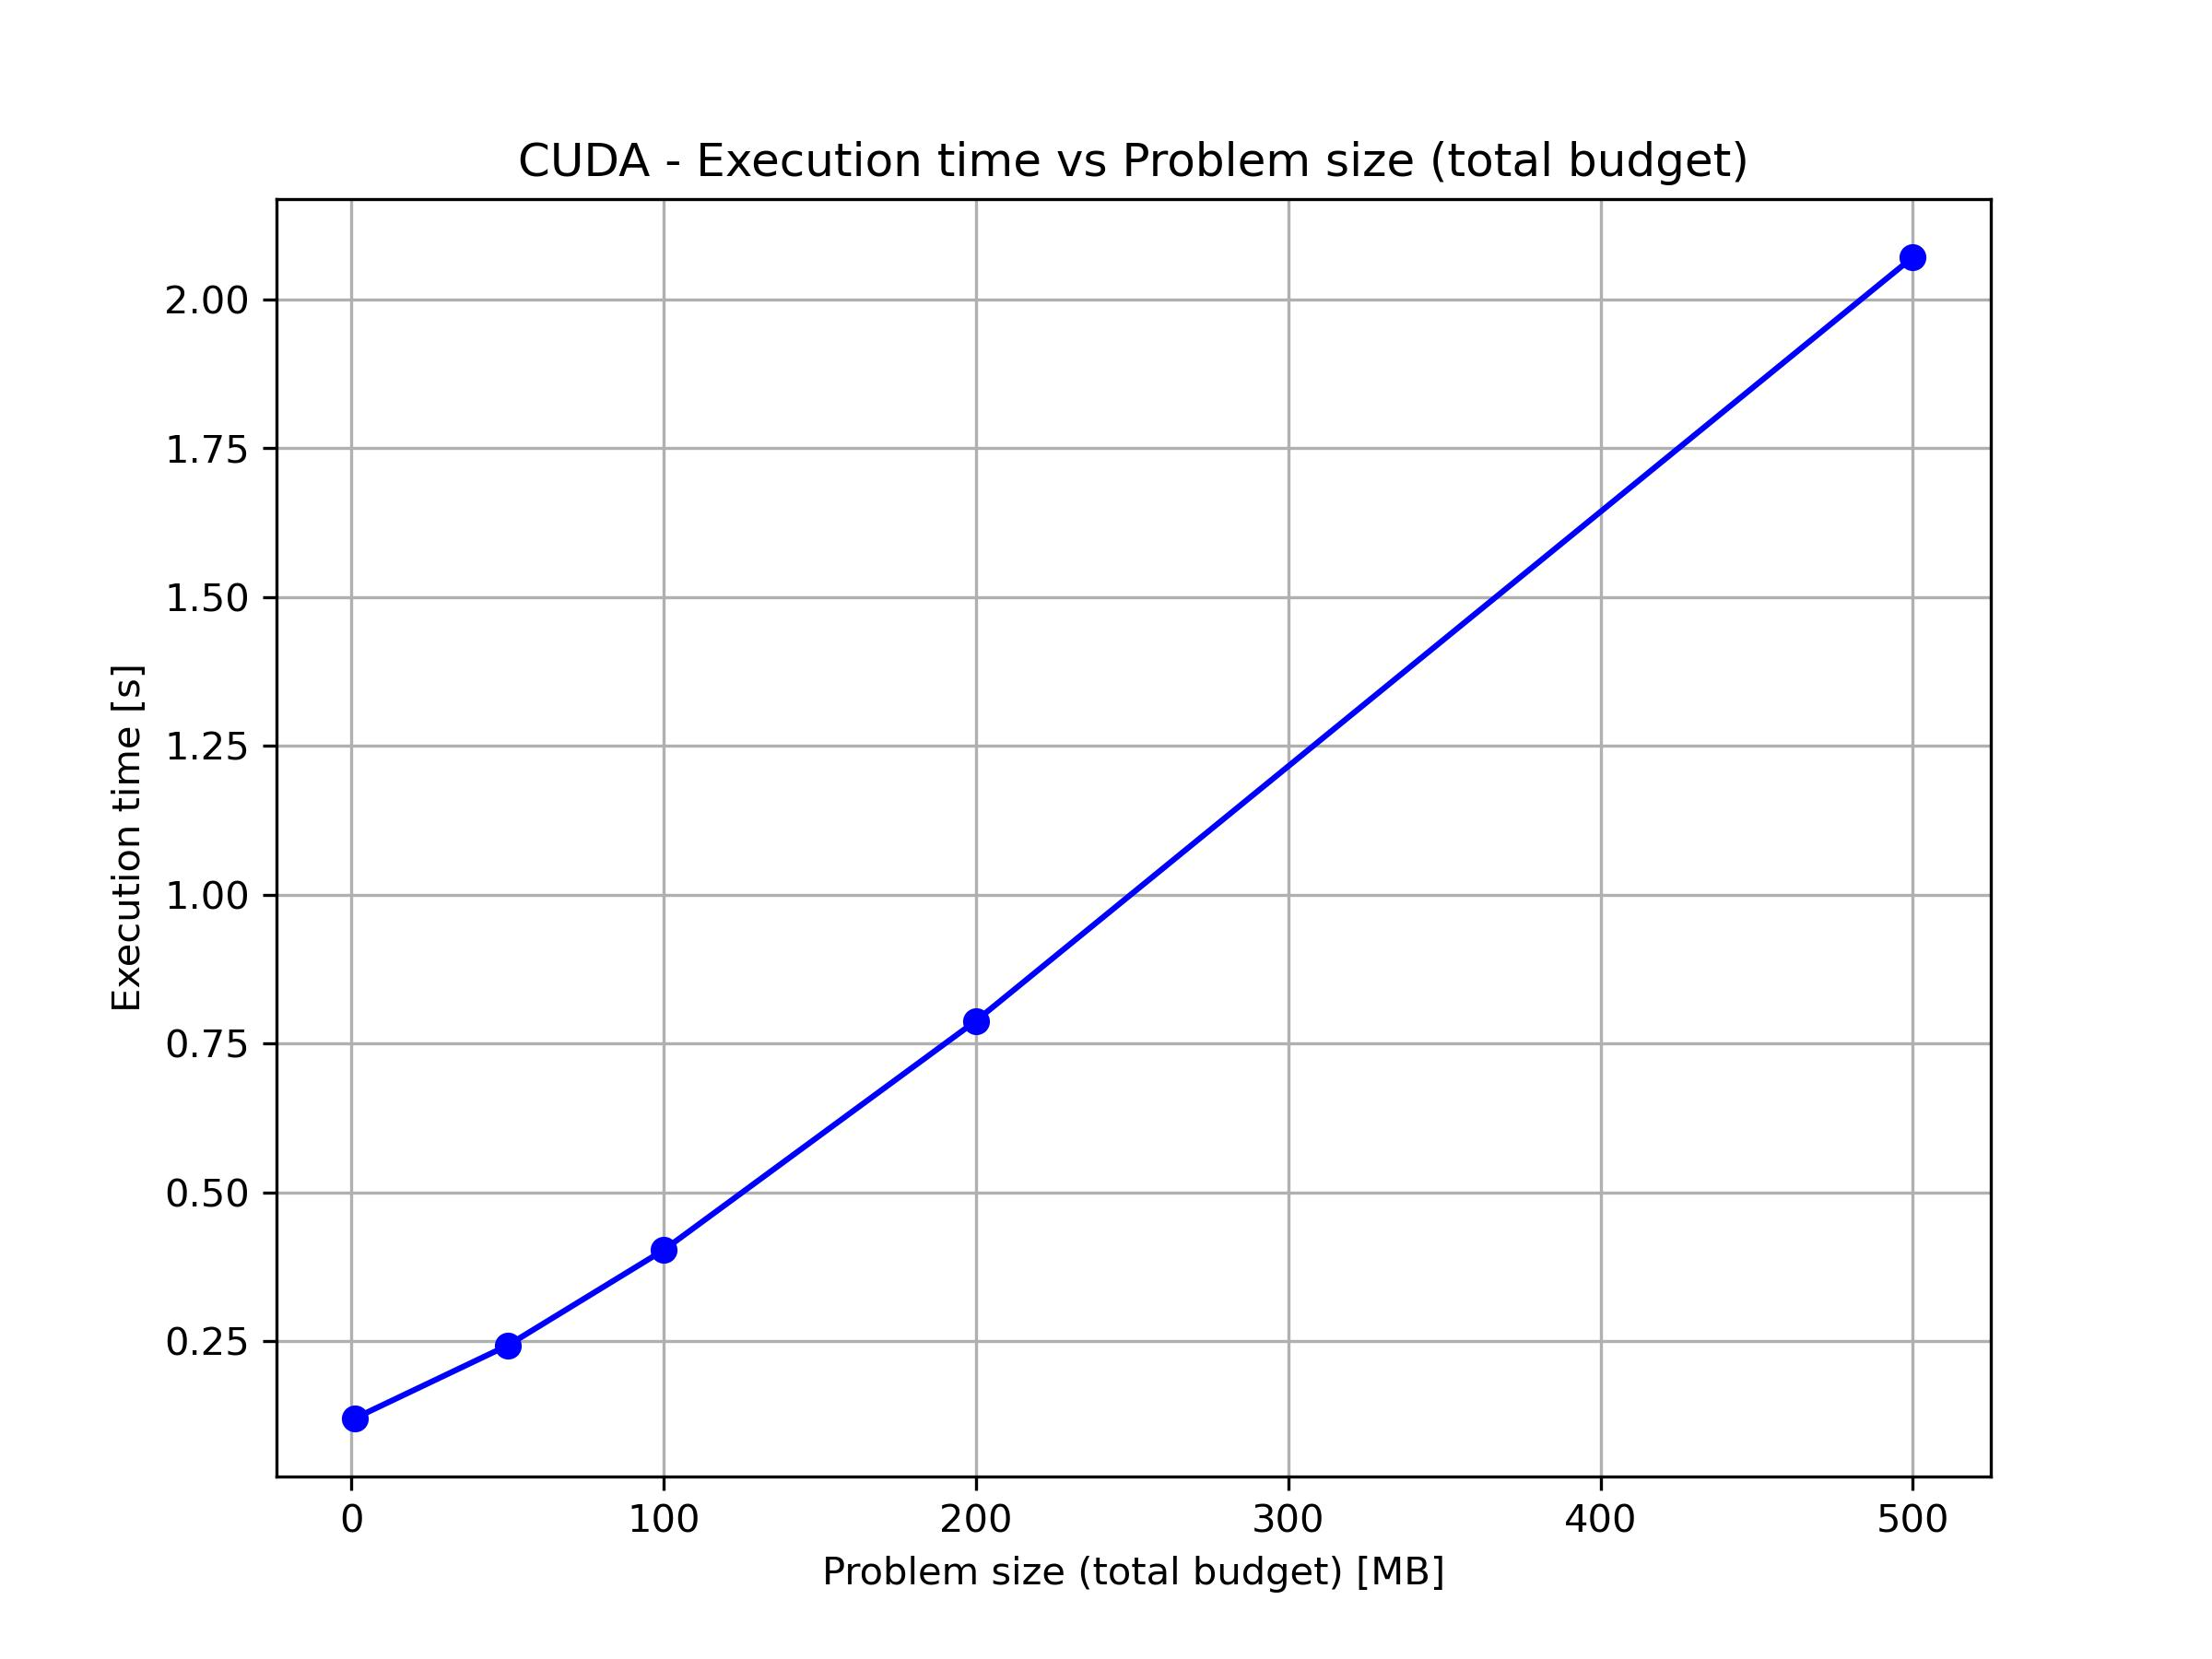
\includegraphics[width=\textwidth]{img/cuda_plots/cuda_times.jpg}
					\caption{Tempi CUDA}
					\label{fig:cuda_times}
				\end{minipage}
				\hfill
				\begin{minipage}[t]{0.49\textwidth}
					\centering
					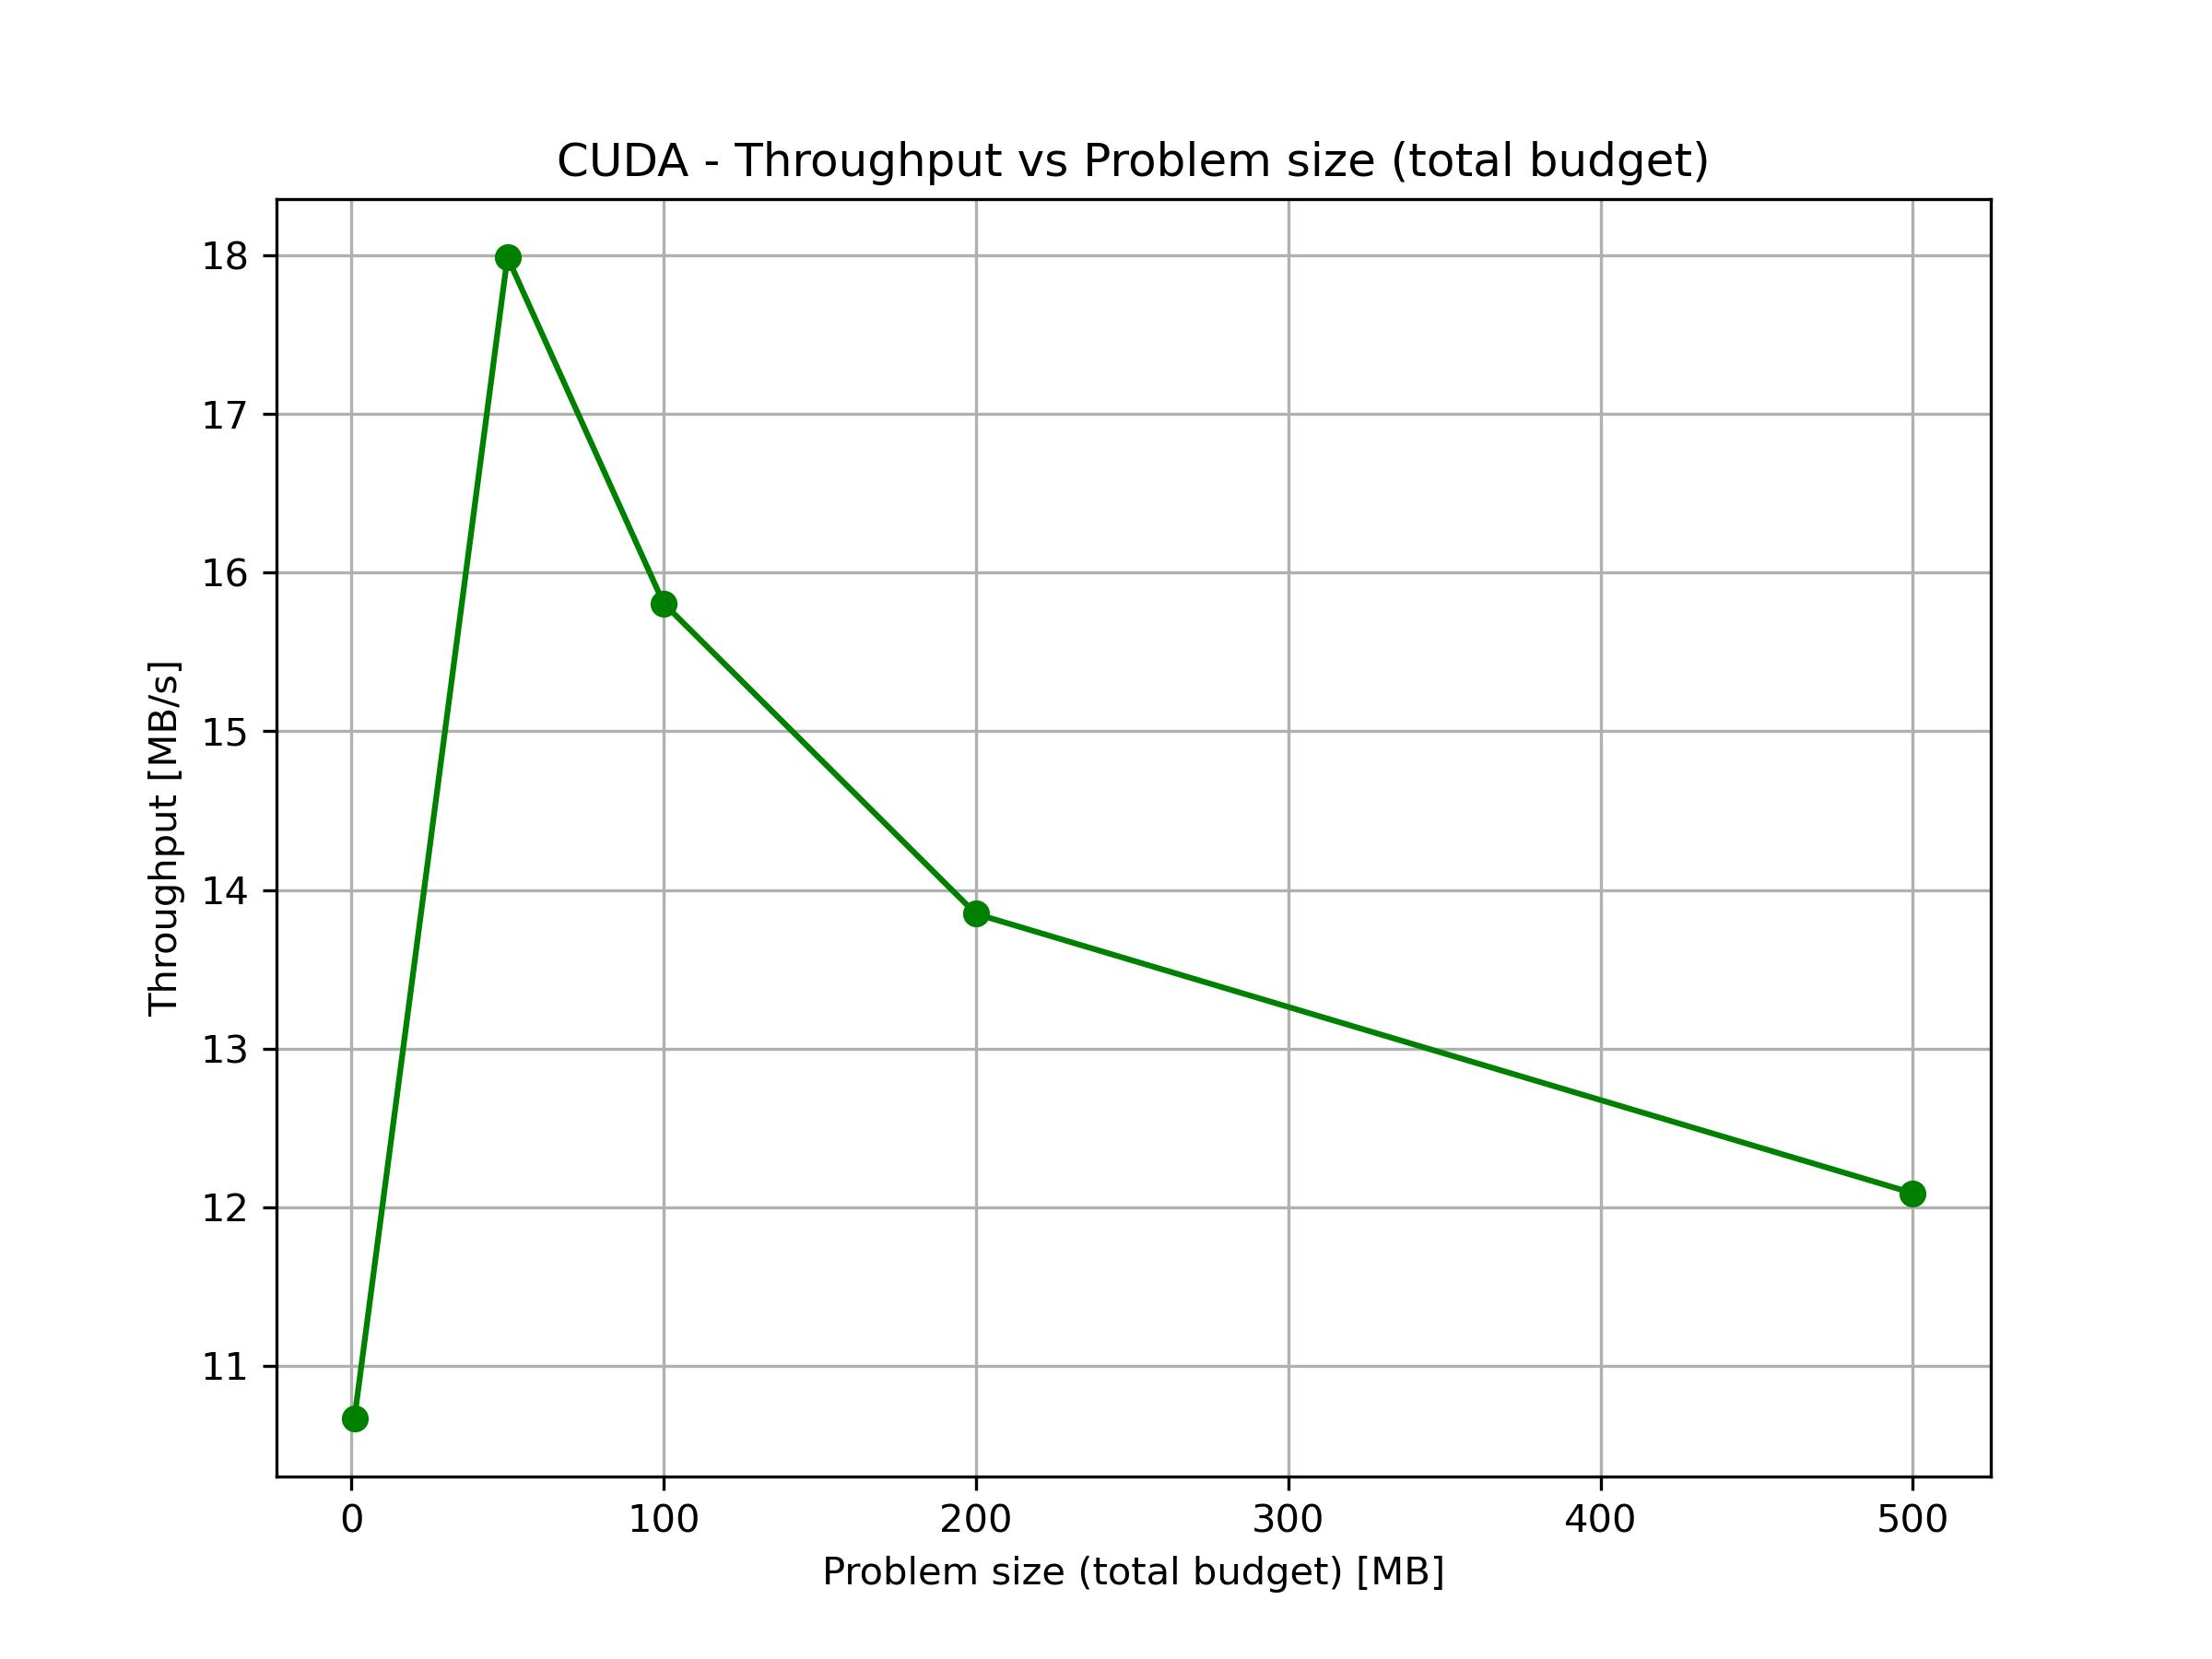
\includegraphics[width=\textwidth]{img/cuda_plots/cuda_throughput.jpg}
					\caption{Throughput CUDA}
					\label{fig:cuda_throughput}
				\end{minipage}
			\end{figure}
			
			\begin{figure}[H]
				\centering
				\begin{minipage}[t]{0.49\textwidth}
					\centering
					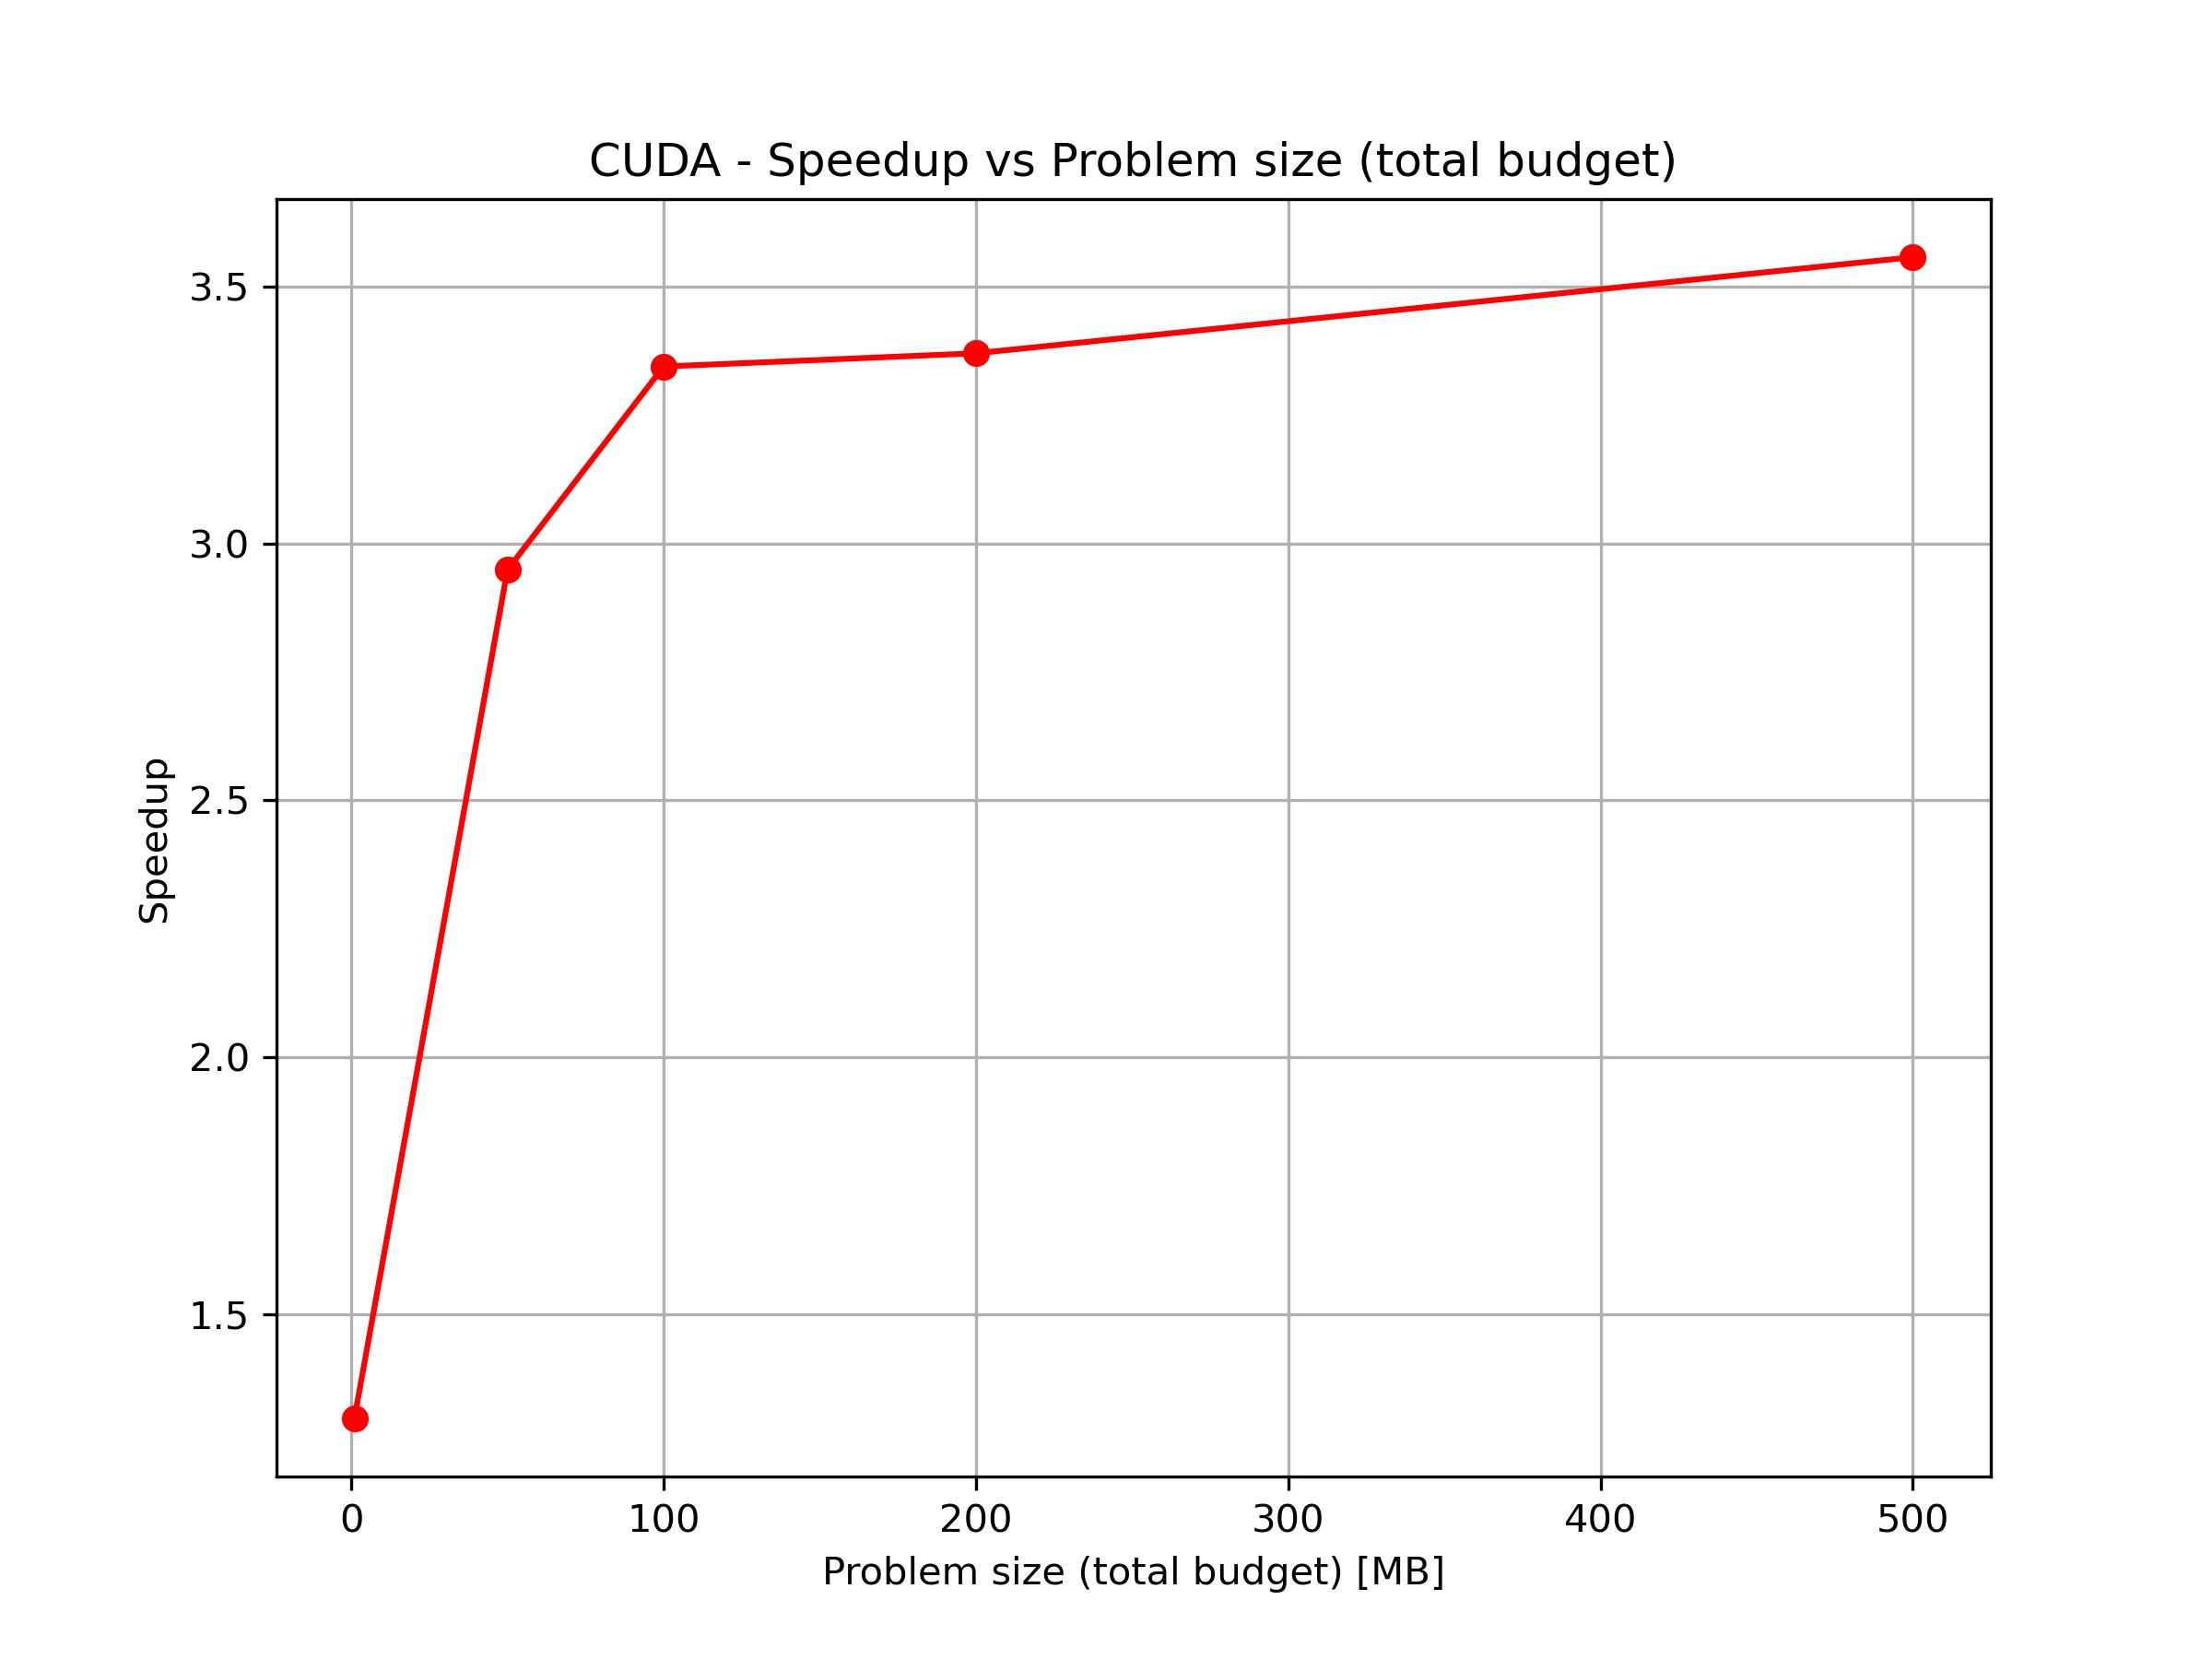
\includegraphics[width=\textwidth]{img/cuda_plots/cuda_speedup.jpg}
					\caption{Speedup CUDA}
					\label{fig:cuda_speedup}
				\end{minipage}
				\hfill
				\begin{minipage}[t]{0.49\textwidth}
					\centering
					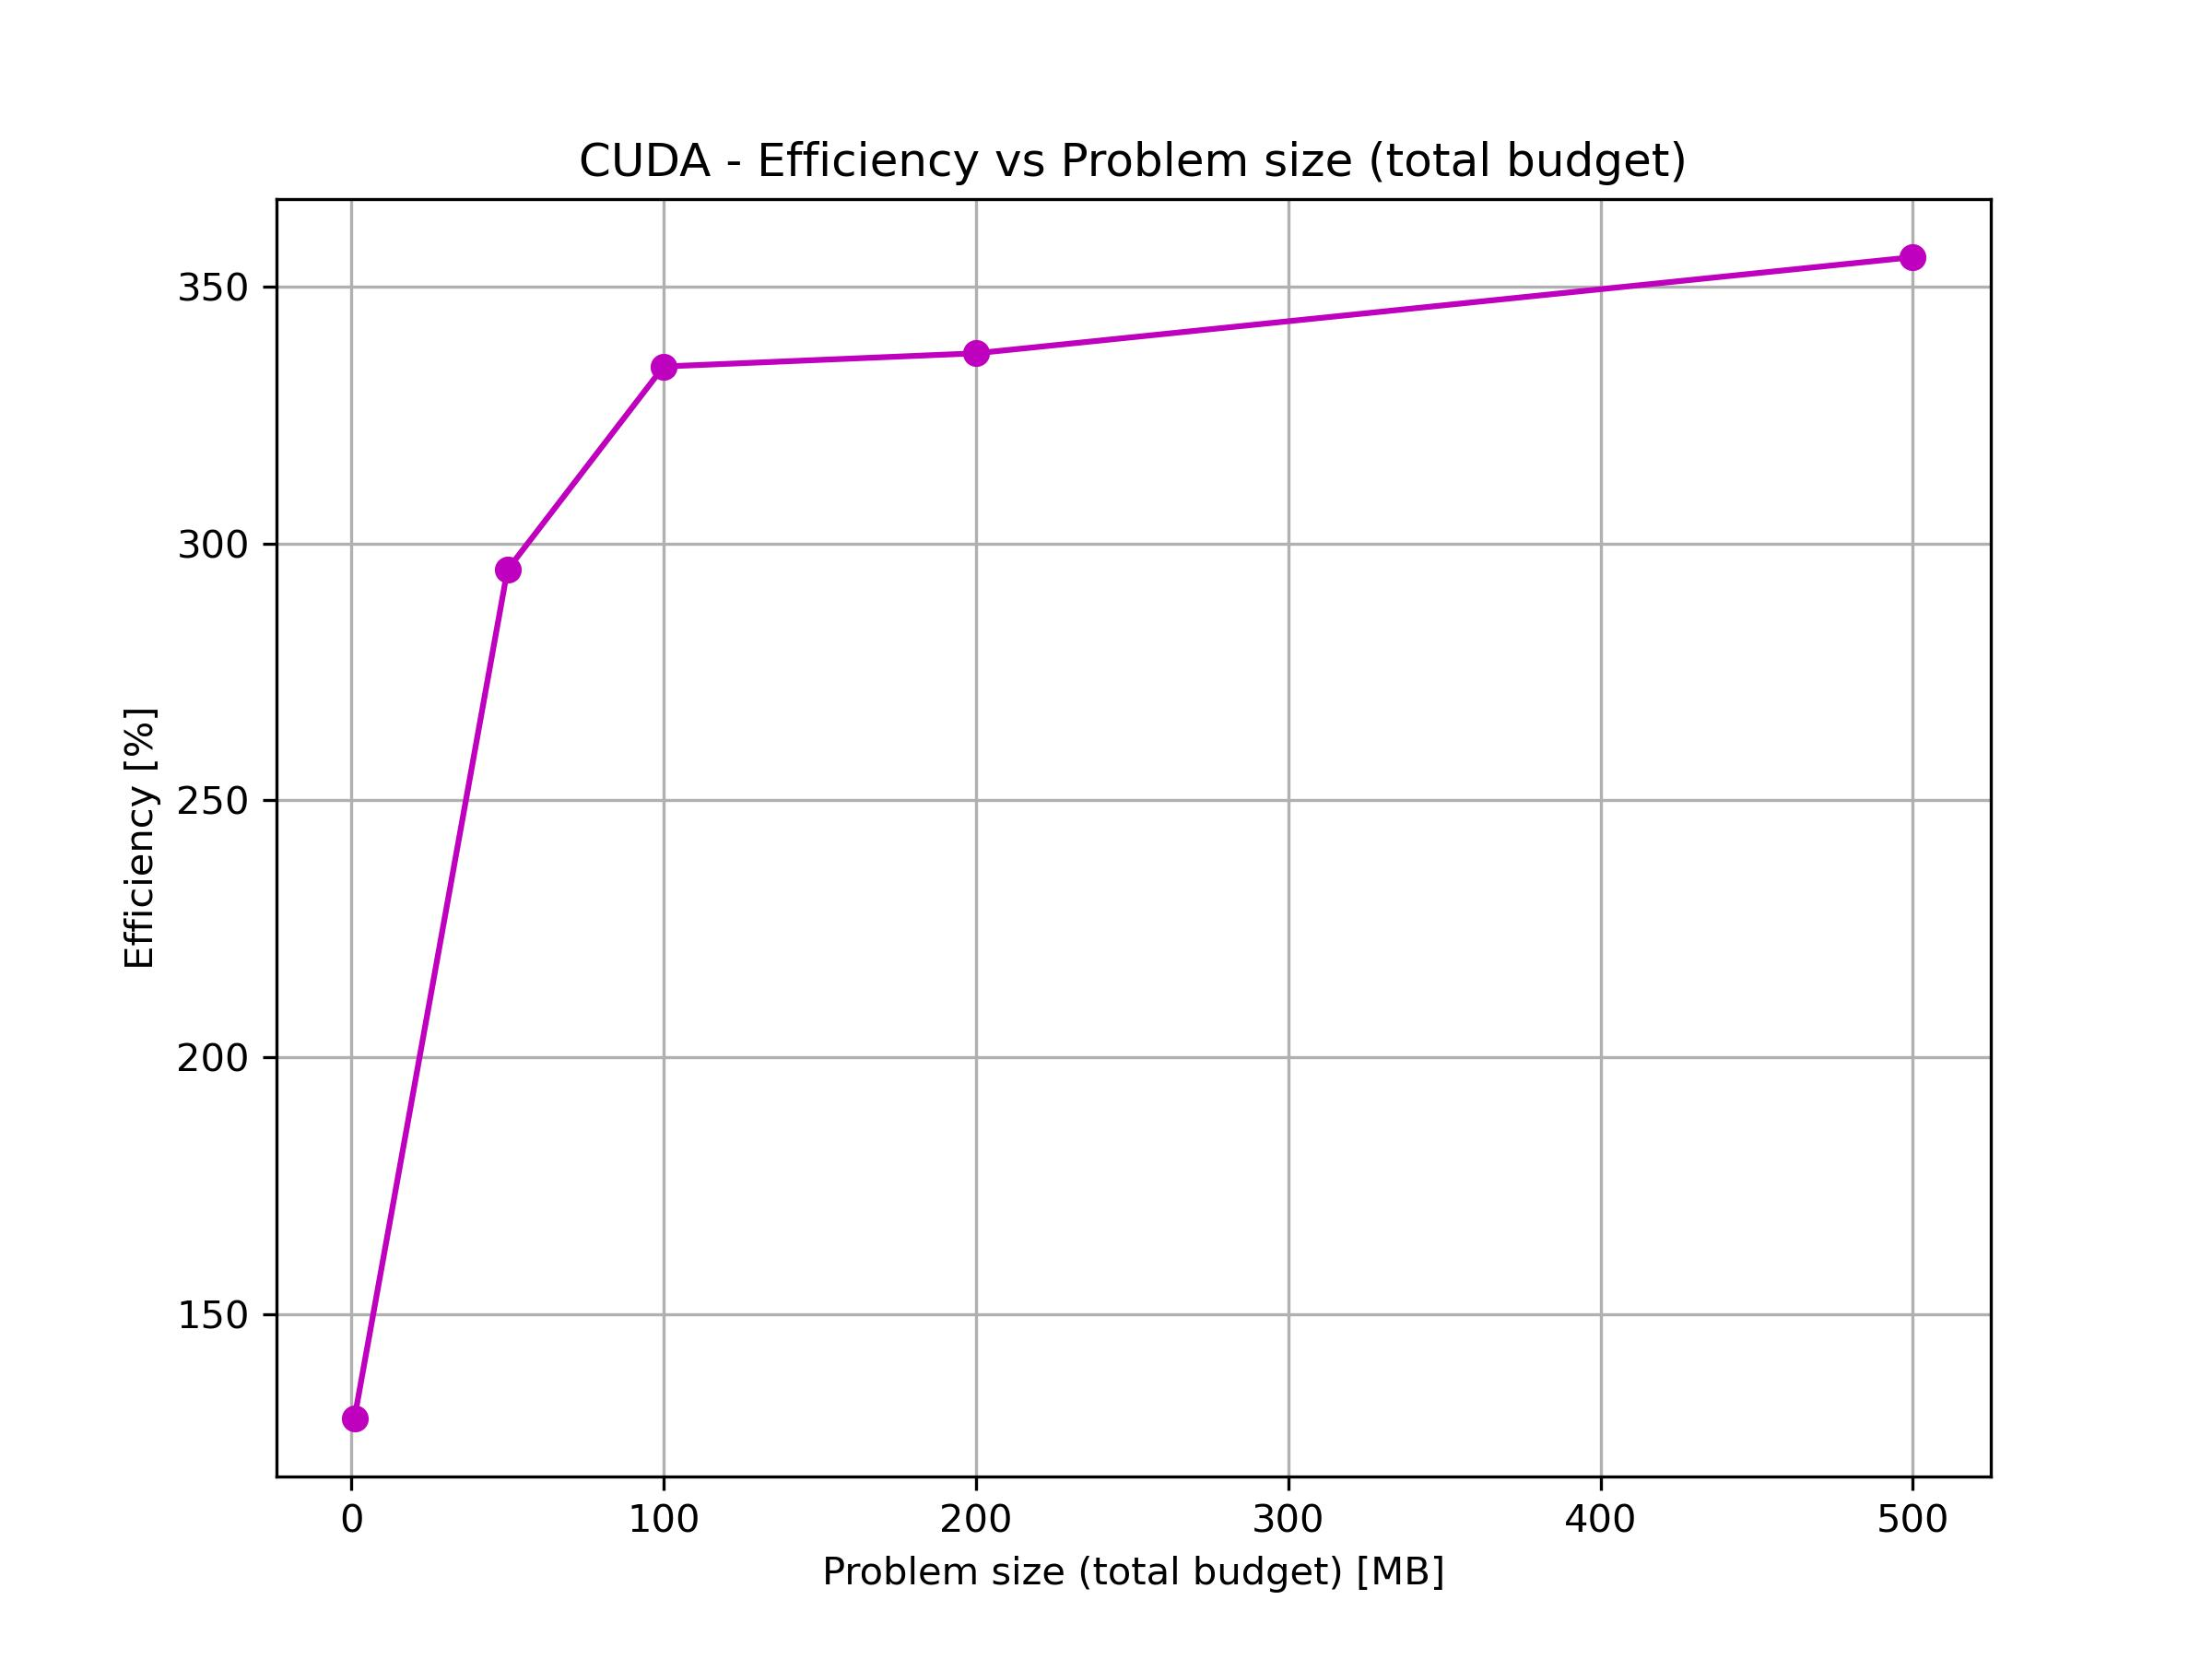
\includegraphics[width=\textwidth]{img/cuda_plots/cuda_efficiency.jpg}
					\caption{Efficiency CUDA}
					\label{fig:cuda_efficiency}
				\end{minipage}
			\end{figure}
			
			\subsubsection*{Osservazioni}
				\begin{itemize}
						\item Il tempo è dominato dal \textbf{kernel GPU} e dalla \textbf{costruzione LCP su CPU}: a 500 MB il kernel impiega \(\sim 0.85\) s (\(\sim 43\%\)) e LCP \(\sim 1.12\) s (\(\sim 54\%\)).
						\item Le \textbf{transfer} (\(\text{H2D}+\text{D2H}\)) restano marginali: \(\sim 0.06\) s su 2.07 s totali (\(<3\%\)).
						\item Il \textbf{throughput} cala con l’aumento della dimensione: da \(\sim 18\) MB/s (50 MB) a \(\sim 12\) MB/s (500 MB).
						\item Lo \textbf{speedup} medio rispetto al sequenziale è \(\sim 3.3{-}3.6\times\) per input grandi.
				\end{itemize}
		
		\subsection{Profiling della memoria}
			Il profilo a 500 MB è stato approfondito con \texttt{ncu} (\textit{Nsight Compute}) usando \texttt{ncu\_cuda\_profile.sh}.
			Nel run profilato (\texttt{cuda\_500MB\_profile.txt/.ncu-rep}) si osservano:
			\begin{itemize}
				\item \texttt{time\_kernel\_gpu} \(\approx 0.857\) s,
				\item \texttt{time\_lcp\_cpu} \(\approx 1.106\) s,
				\item \texttt{time\_h2d} \(\approx 0.004\) s, \texttt{time\_d2h} \(\approx 0.055\) s \(\Rightarrow\) transfer complessive \(\sim 0.06\) s (\(\sim 2.8\%\) del compute),
				\item \texttt{time\_alloc\_host\_dev}: \(\sim 0.10\) s nelle medie, ma fino a \(>2\) s con \texttt{ncu} per effetto dell’overhead dello strumento.
			\end{itemize}
			
			\subsubsection*{Footprint in memoria}
				Nel caso single-stream, il footprint è dato da:
				\begin{enumerate}
						\item \textbf{Buffer del testo} su device (\(\sim n\) byte) e relativa copia host (pinned).
						\item \textbf{Array ausiliari} per il SA/LRS su GPU (\(O(n)\) interi a 32 bit).
						\item \textbf{Strutture LCP su CPU} (\(O(n)\) interi) per la \emph{Kasai} finale.
				\end{enumerate}
				Il rapporto \texttt{memory\_overhead\_ratio} decresce con l’input: da \(\sim 96\%\) (1 MB, dominato da overhead fissi) a \(\sim 8\%\) (500 MB).
				
				\begin{figure}[H]
						\centering
						\begin{minipage}[t]{0.49\textwidth}
							\centering
							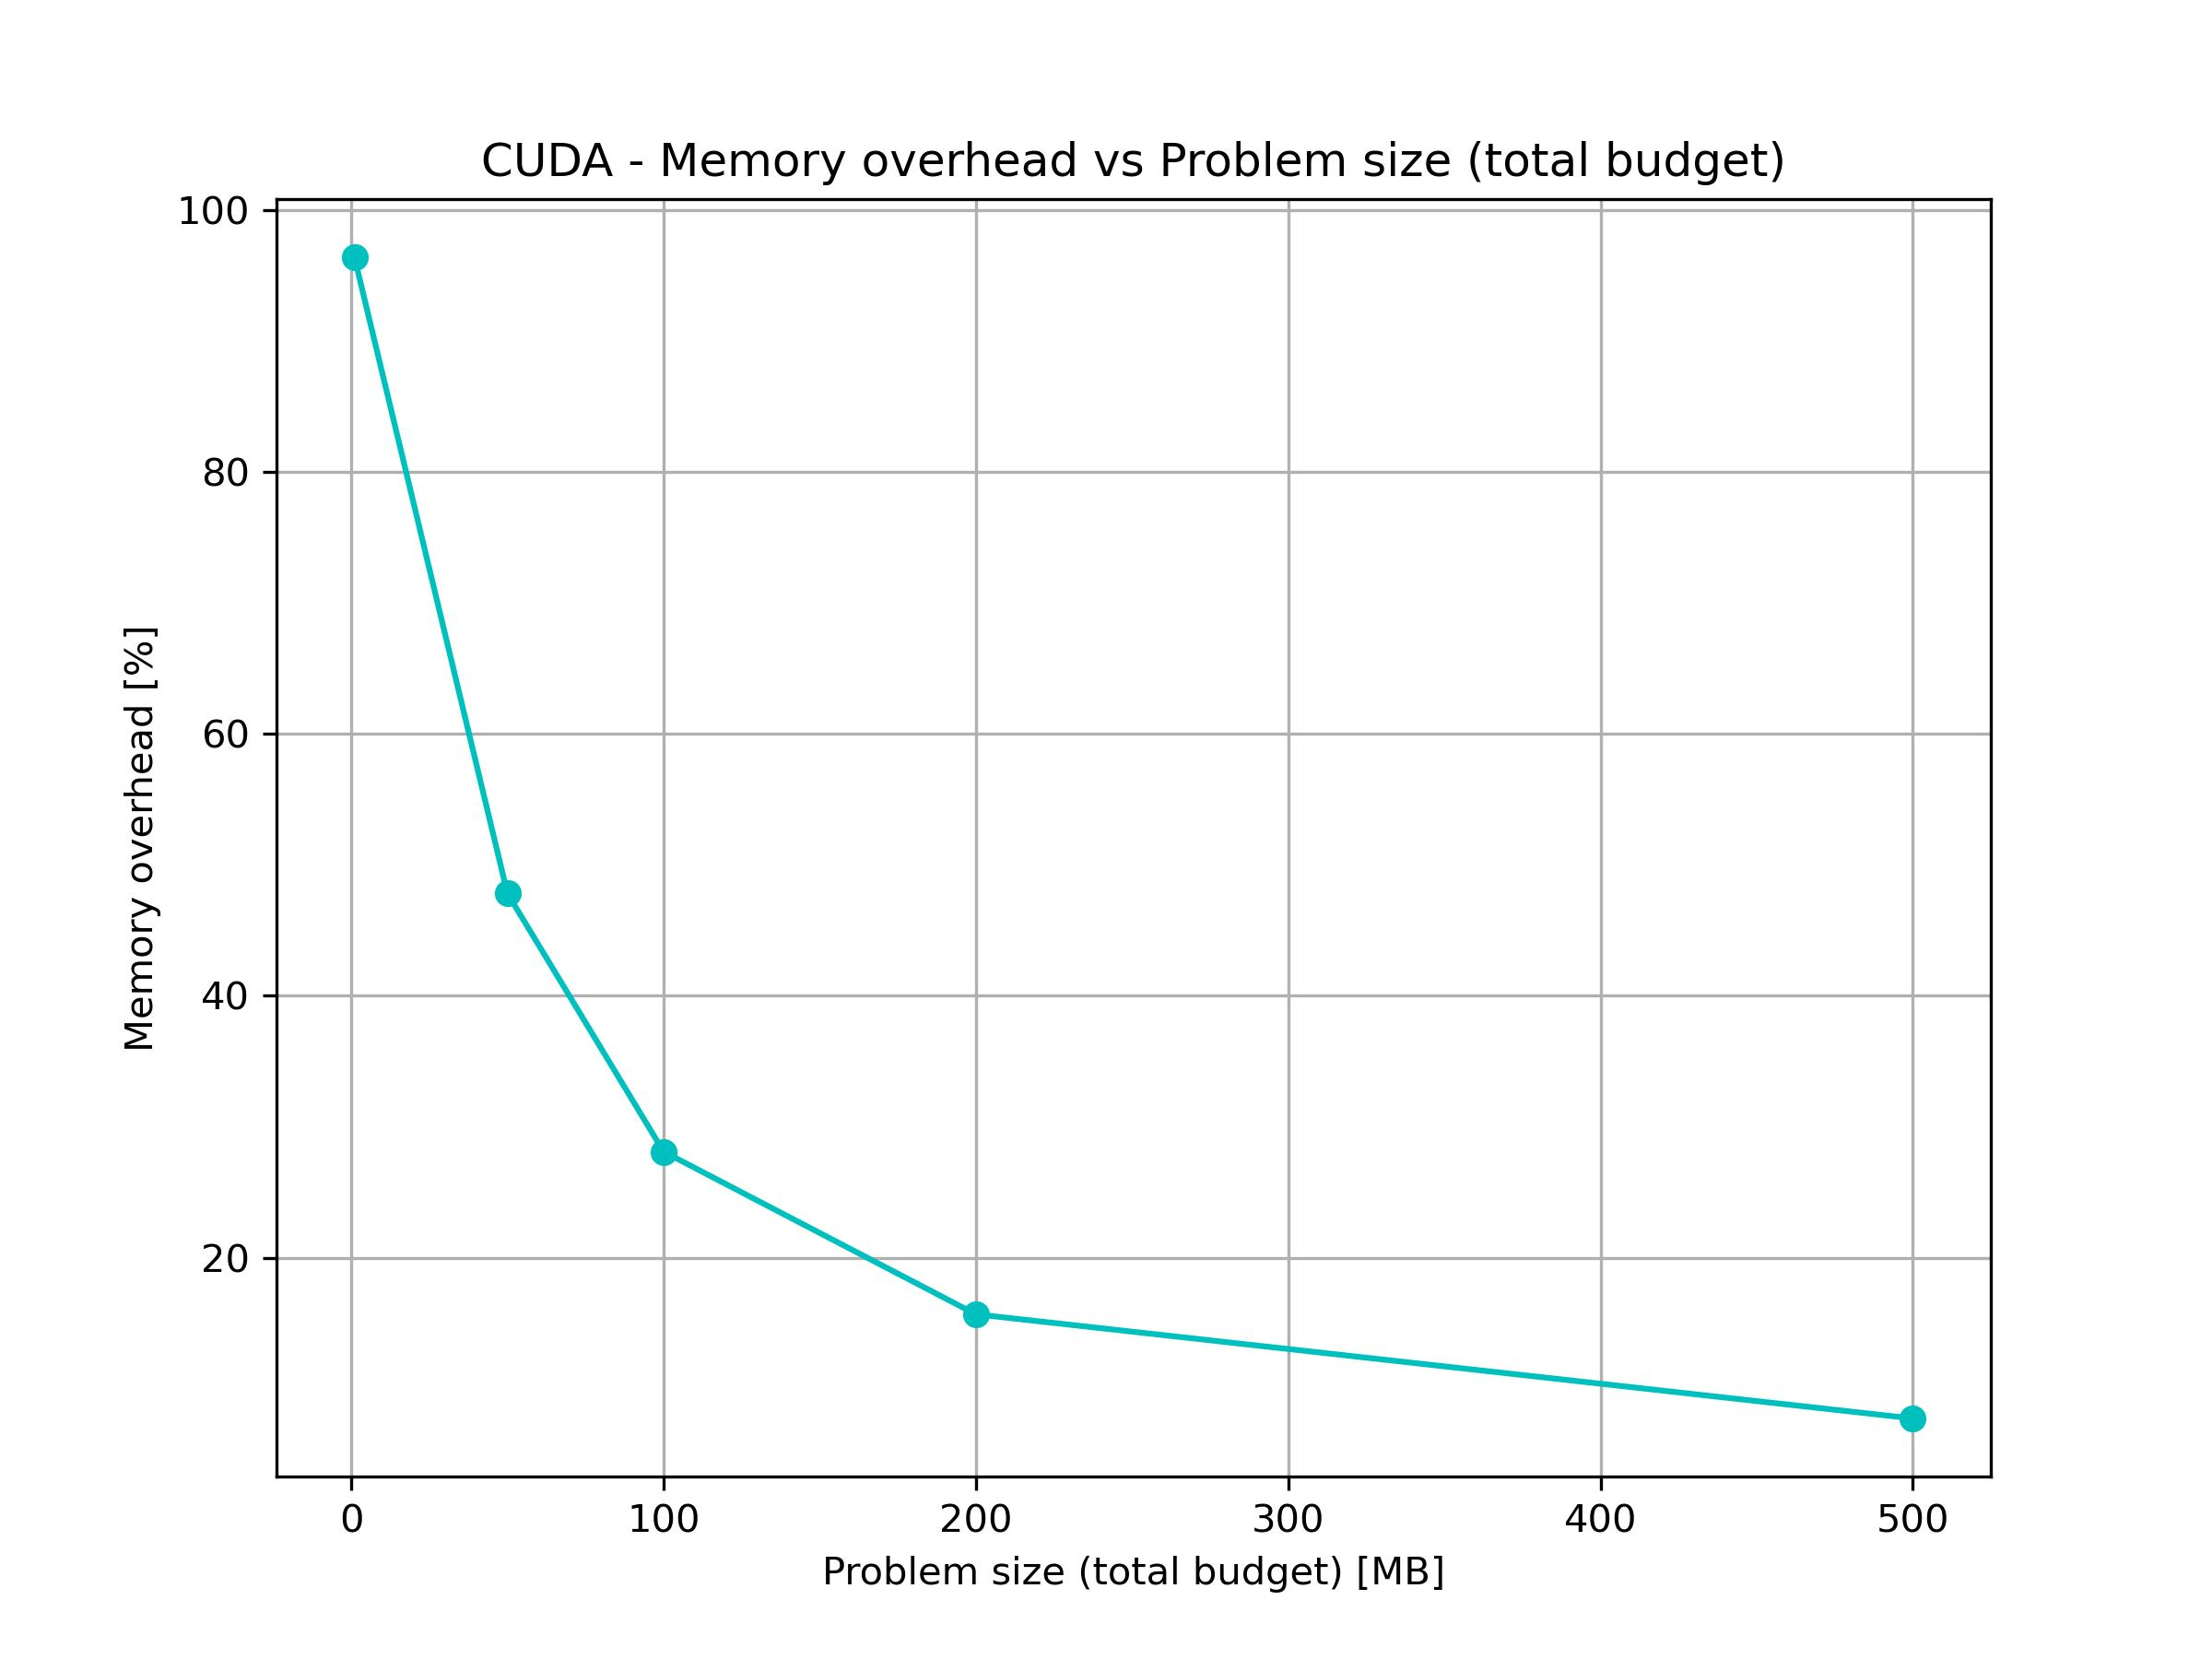
\includegraphics[width=\textwidth]{img/cuda_plots/cuda_memory_overhead.jpg}
							\caption{Memory overhead CUDA}
							\label{fig:cuda_mem_overhead}
						\end{minipage}
						\hfill
						\begin{minipage}[t]{0.49\textwidth}
							\centering
							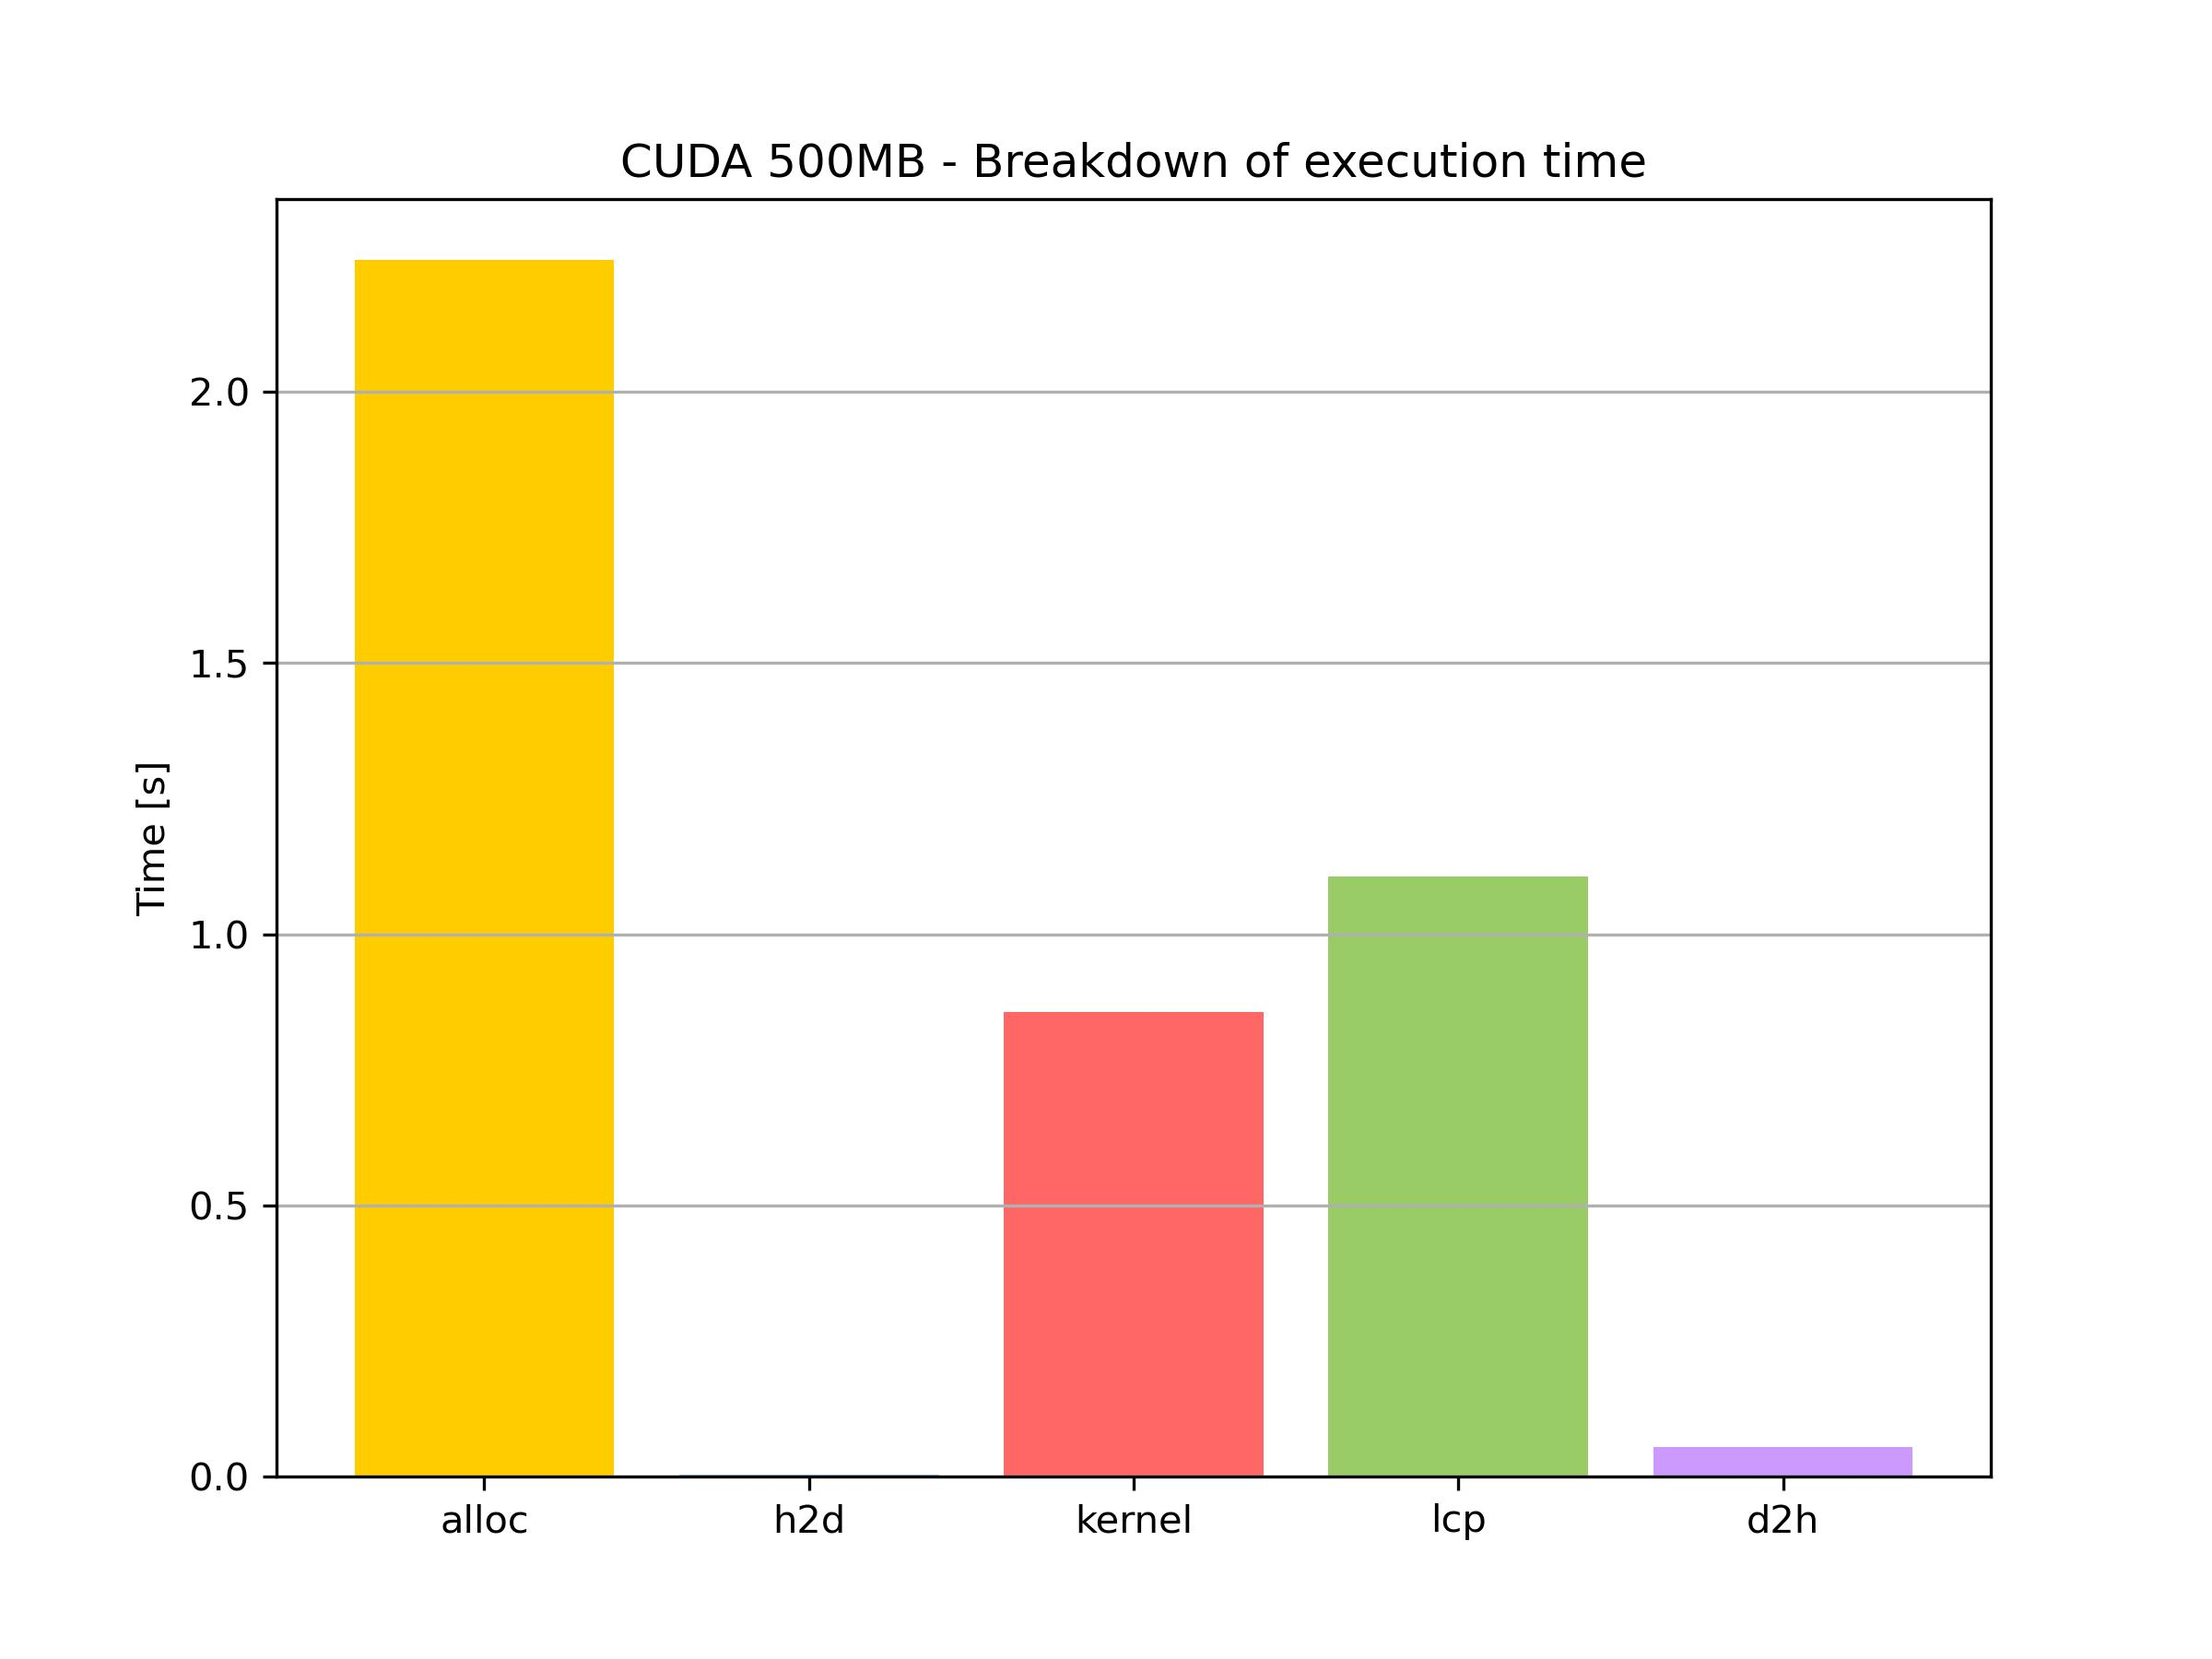
\includegraphics[width=\textwidth]{img/cuda_plots/cuda_breakdown_100MB.jpg}
							\caption{Breakdown CUDA}
							\label{fig:cuda_breakdown}
						\end{minipage}
				\end{figure}
			
			\subsubsection*{Conclusioni}
				\begin{itemize}
						\item La pipeline è \emph{compute-bound}: kernel e LCP dominano, trasferimenti PCIe trascurabili.
						\item L’overhead di allocazione è ridotto nei run reali (\(\sim 0.1\) s), ma amplificato sotto profiling.
						\item Il footprint scala lineare con \(n\): \(O(n)\) su device (testo + array interi) e \(O(n)\) su host (LCP).
						\item Il modello single-stream non richiede buffer extra per overlap, risultando più semplice da gestire in memoria.
				\end{itemize}
	
	\section{Versione CUDA \emph{multi-stream}}
		
		\subsection{Analisi dei tempi}
			
			I benchmark sono stati eseguiti con \texttt{cuda\_ms\_measure.sh} su input da \(\{1,50,100,200,500\}\) MB e con \(\{2,4,8\}\) stream, 10 run ciascuno.
			I file \texttt{cuda\_ms\_summary.csv} riportano i valori medi per ciascuna coppia \emph{size\(\times\)streams}.
			
			\begin{table}[h]
				\centering
				\scriptsize
				\setlength{\tabcolsep}{5pt}
				\resizebox{\textwidth}{!} \\
						\textbf{(MB)} & & \textbf{(s)} & \textbf{(s)} & \textbf{(s)} & \textbf{(s)} & \textbf{(s)} & \textbf{pure (s)} & \textbf{compute (s)} & \textbf{(s)} \\
						\midrule
						1                   & 2             & 0.112          & 0.00002      & 0.0109          & 0.00047           & 0.00605      & 0.0114           & 0.124          & 0.00607       & 4.18          & 0.51             & 50.9              \\
						1                   & 4             & 0.111          & 0.00002      & 0.0161          & 0.00045           & 0.00605      & 0.0165           & 0.128          & 0.00607       & 2.88          & 0.35             & 35.0              \\
						1                   & 8             & 0.111          & 0.00002      & 0.0258          & 0.00045           & 0.00604      & 0.0262           & 0.137          & 0.00606       & 1.82          & 0.22             & 22.1              \\
						\midrule
						50                  & 2             & 0.104          & 0.00031      & 0.253           & 0.0566            & 0.535        & 0.310            & 0.414          & 0.535         & 7.69          & 1.26             & 126               \\
						50                  & 4             & 0.103          & 0.00031      & 0.224           & 0.0582            & 0.530        & 0.283            & 0.386          & 0.531         & 8.42          & 1.38             & 138               \\
						50                  & 8             & 0.102          & 0.00031      & 0.242           & 0.0621            & 0.530        & 0.304            & 0.406          & 0.530         & 7.83          & 1.28             & 128               \\
						\midrule
						100                 & 2             & 0.102          & 0.00065      & 0.646           & 0.151             & 1.494        & 0.797            & 0.899          & 1.494         & 5.98          & 1.26             & 126               \\
						100                 & 4             & 0.102          & 0.00066      & 0.599           & 0.156             & 1.494        & 0.755            & 0.857          & 1.494         & 6.31          & 1.33             & 133               \\
						100                 & 8             & 0.102          & 0.00066      & 0.552           & 0.153             & 1.494        & 0.705            & 0.807          & 1.494         & 6.75          & 1.43             & 143               \\
						\midrule
						200                 & 2             & 0.102          & 0.00143      & 1.615           & 0.384             & 3.521        & 1.999            & 2.101          & 3.523         & 4.76          & 1.16             & 116               \\
						200                 & 4             & 0.103          & 0.00143      & 1.521           & 0.389             & 3.532        & 1.910            & 2.013          & 3.533         & 4.99          & 1.21             & 121               \\
						200                 & 8             & 0.102          & 0.00142      & 1.446           & 0.378             & 3.538        & 1.824            & 1.927          & 3.539         & 5.22          & 1.27             & 127               \\
						\midrule
						500                 & 2             & 0.102          & 0.00366      & 4.744           & 1.168             & 9.241        & 5.912            & 6.014          & 9.245         & 4.03          & 1.19             & 118               \\
						500                 & 4             & 0.103          & 0.00367      & 4.833           & 1.163             & 9.240        & 5.996            & 6.099          & 9.244         & 3.97          & 1.17             & 117               \\
						500                 & 8             & 0.104          & 0.00366      & 4.652           & 1.175             & 9.260        & 5.827            & 5.931          & 9.263         & 4.09          & 1.20             & 120               \\
						\bottomrule
					\end{tabular}}
				\caption{CUDA \emph{multi-stream} — medie (10 run) per dimensione e numero di stream.}
				\label{tab:cuda-ms-times}
			\end{table}
			
			\begin{figure}[H]
				\centering
				\begin{minipage}[t]{0.49\textwidth}
					\centering
					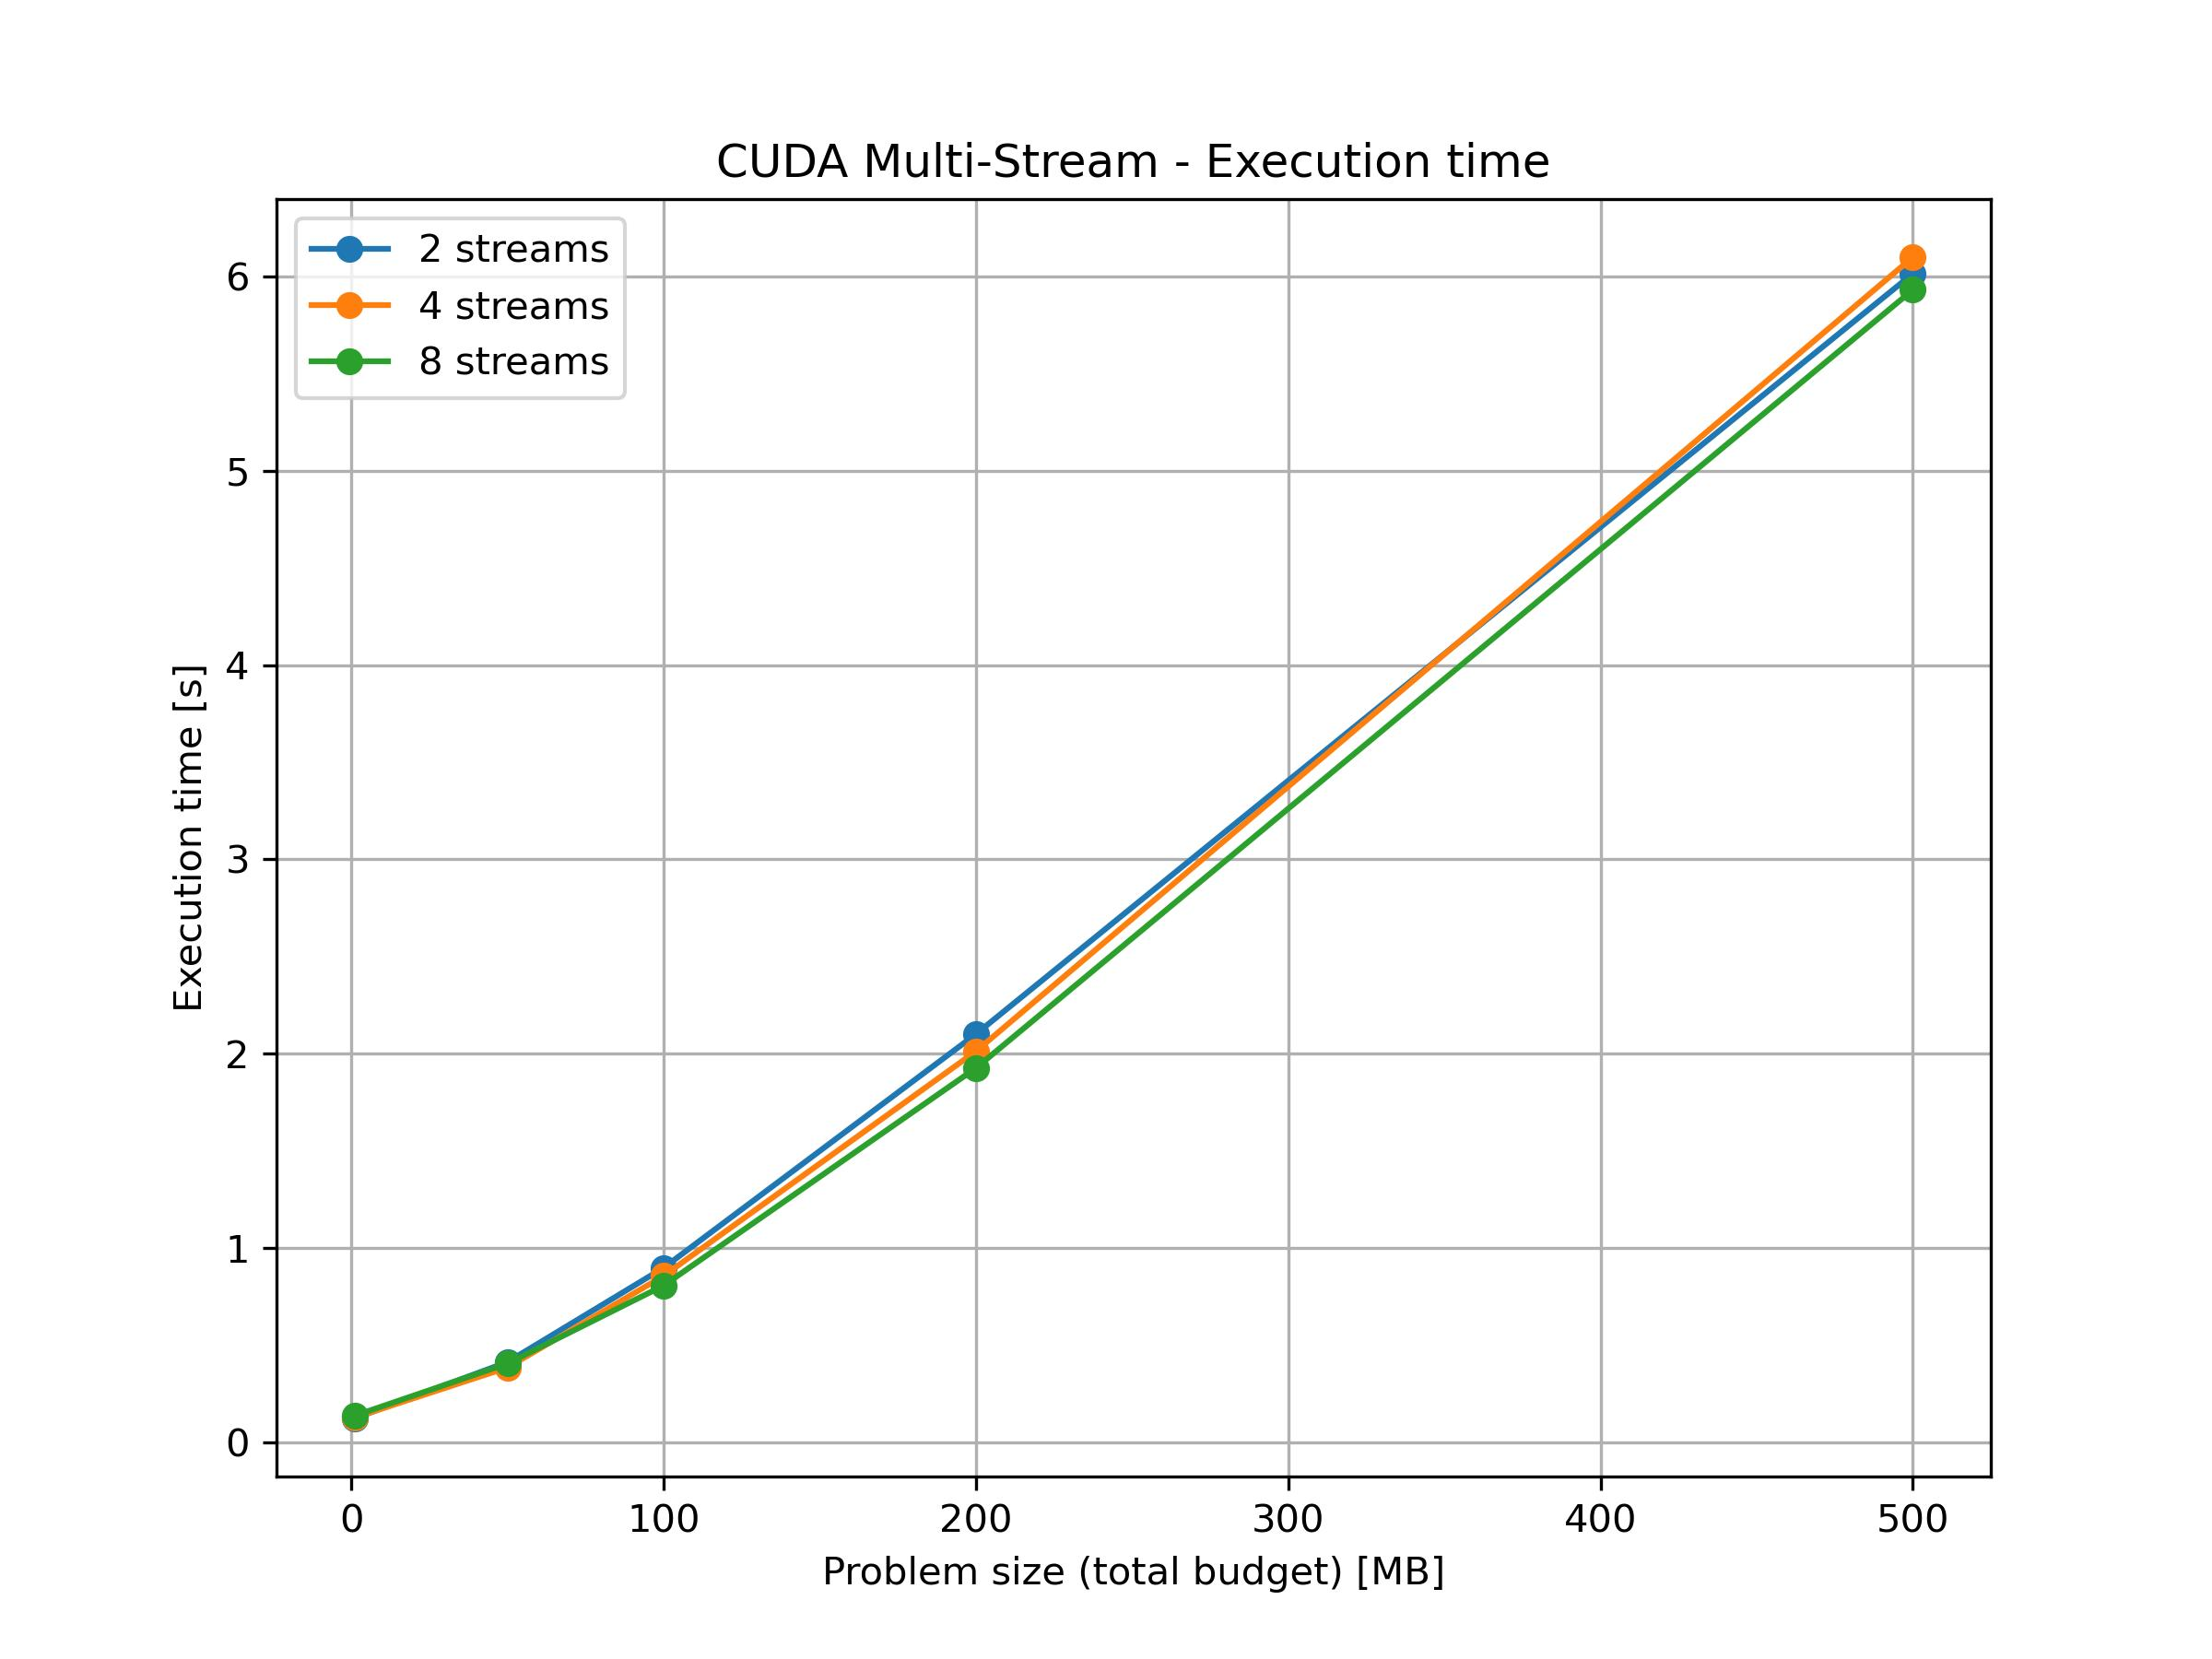
\includegraphics[width=\textwidth]{img/cuda_ms_plots/cuda_ms_times.jpg}
					\caption{Tempi CUDA MS}
					\label{fig:cuda_ms_times}
				\end{minipage}
				\hfill
				\begin{minipage}[t]{0.49\textwidth}
					\centering
					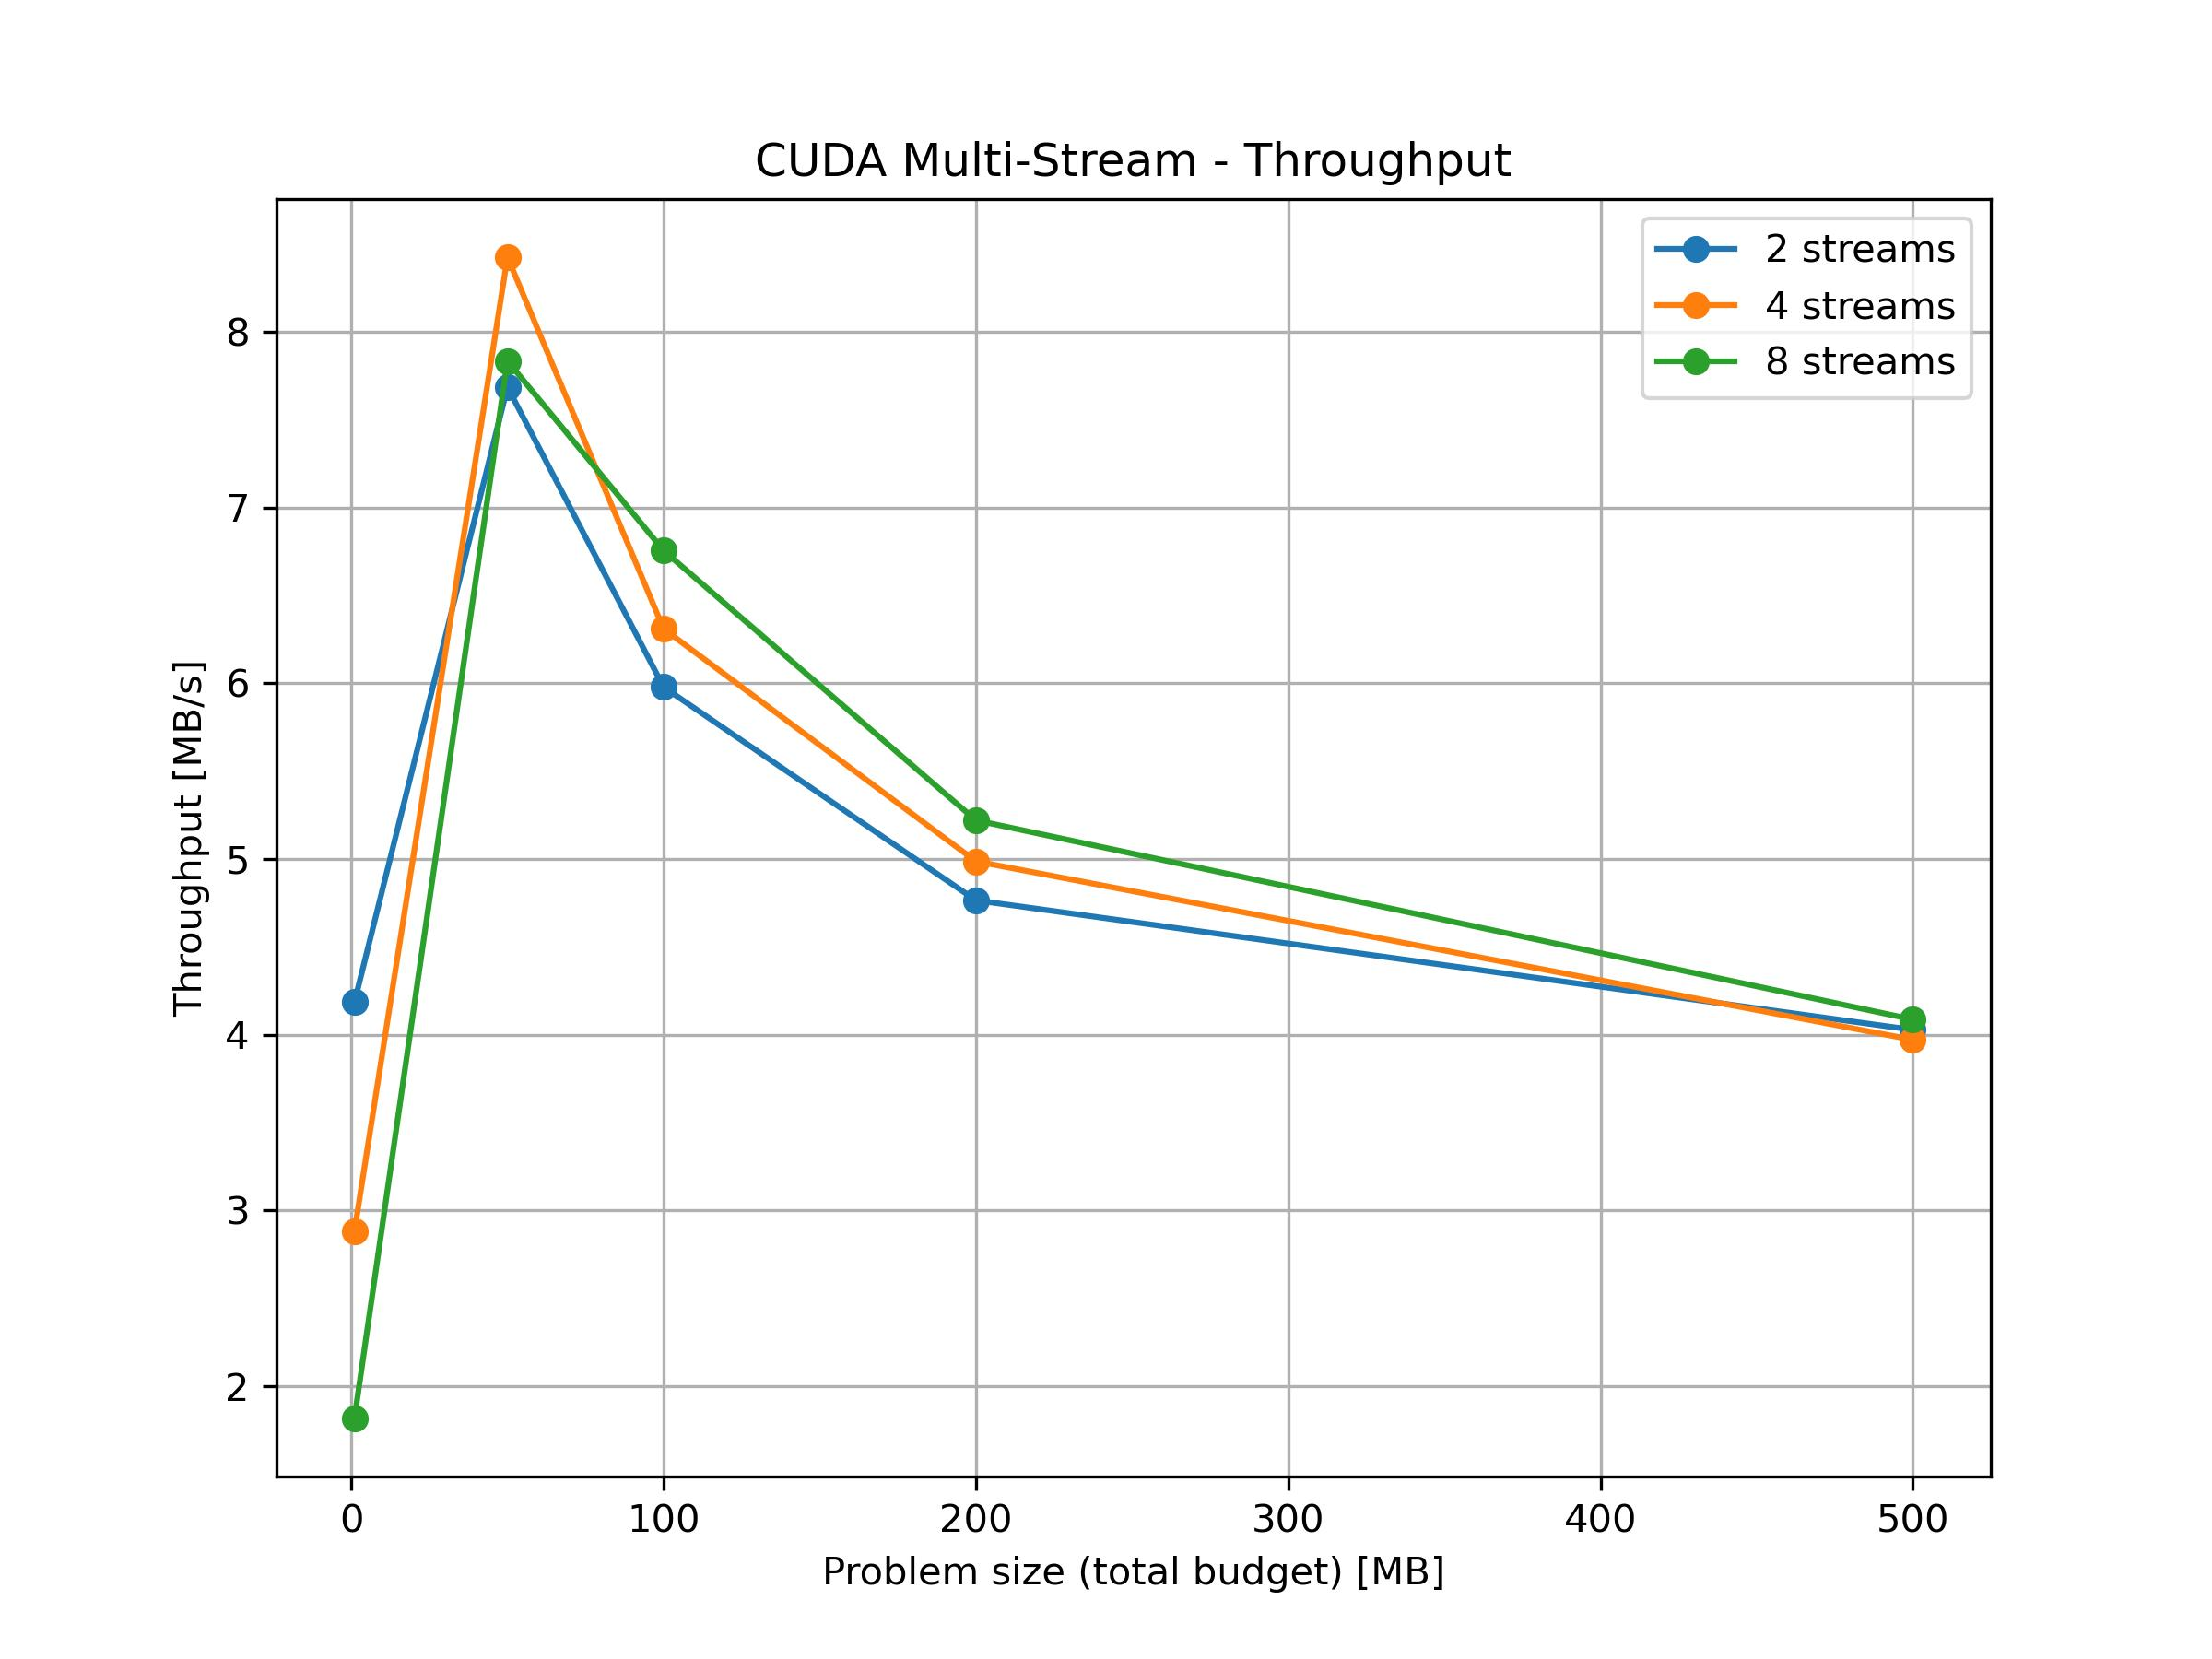
\includegraphics[width=\textwidth]{img/cuda_ms_plots/cuda_ms_throughput.jpg}
					\caption{Throughput CUDA MS}
					\label{fig:cuda_ms_throughput}
				\end{minipage}
			\end{figure}
			
			\begin{figure}[H]
				\centering
				\begin{minipage}[t]{0.49\textwidth}
					\centering
					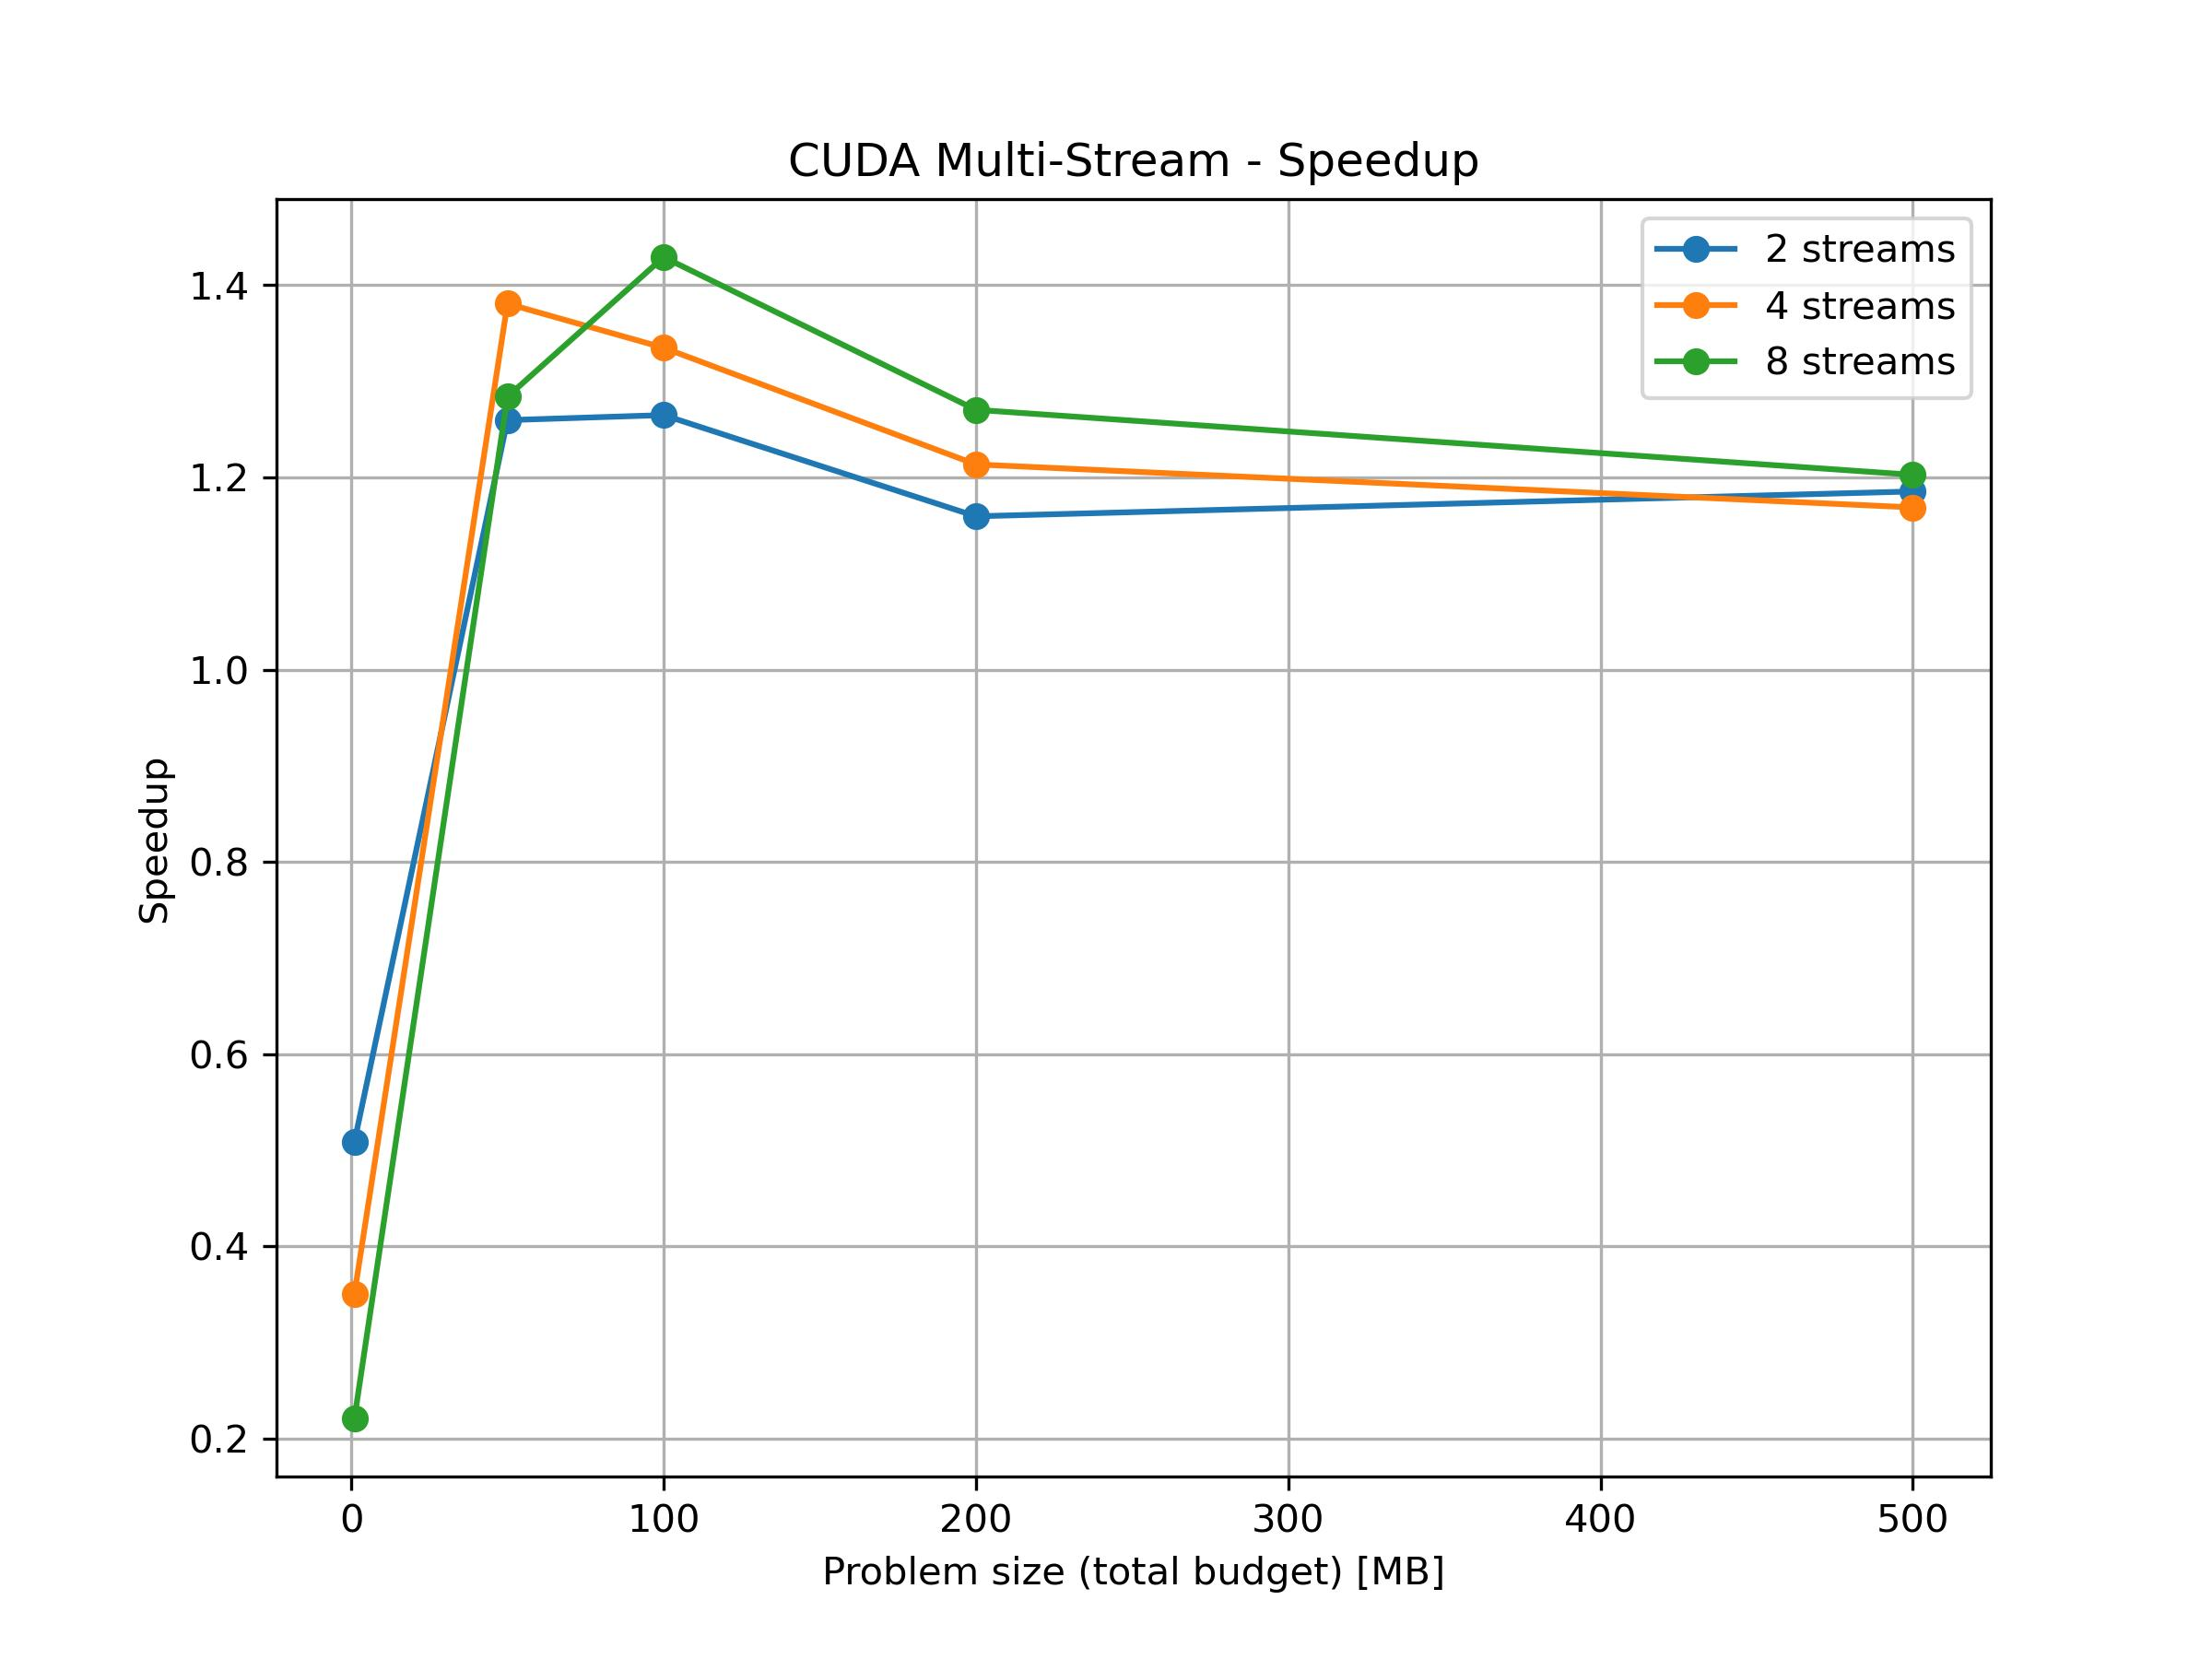
\includegraphics[width=\textwidth]{img/cuda_ms_plots/cuda_ms_speedup.jpg}
					\caption{Speedup CUDA MS}
					\label{fig:cuda_ms_speedup}
				\end{minipage}
				\hfill
				\begin{minipage}[t]{0.49\textwidth}
					\centering
					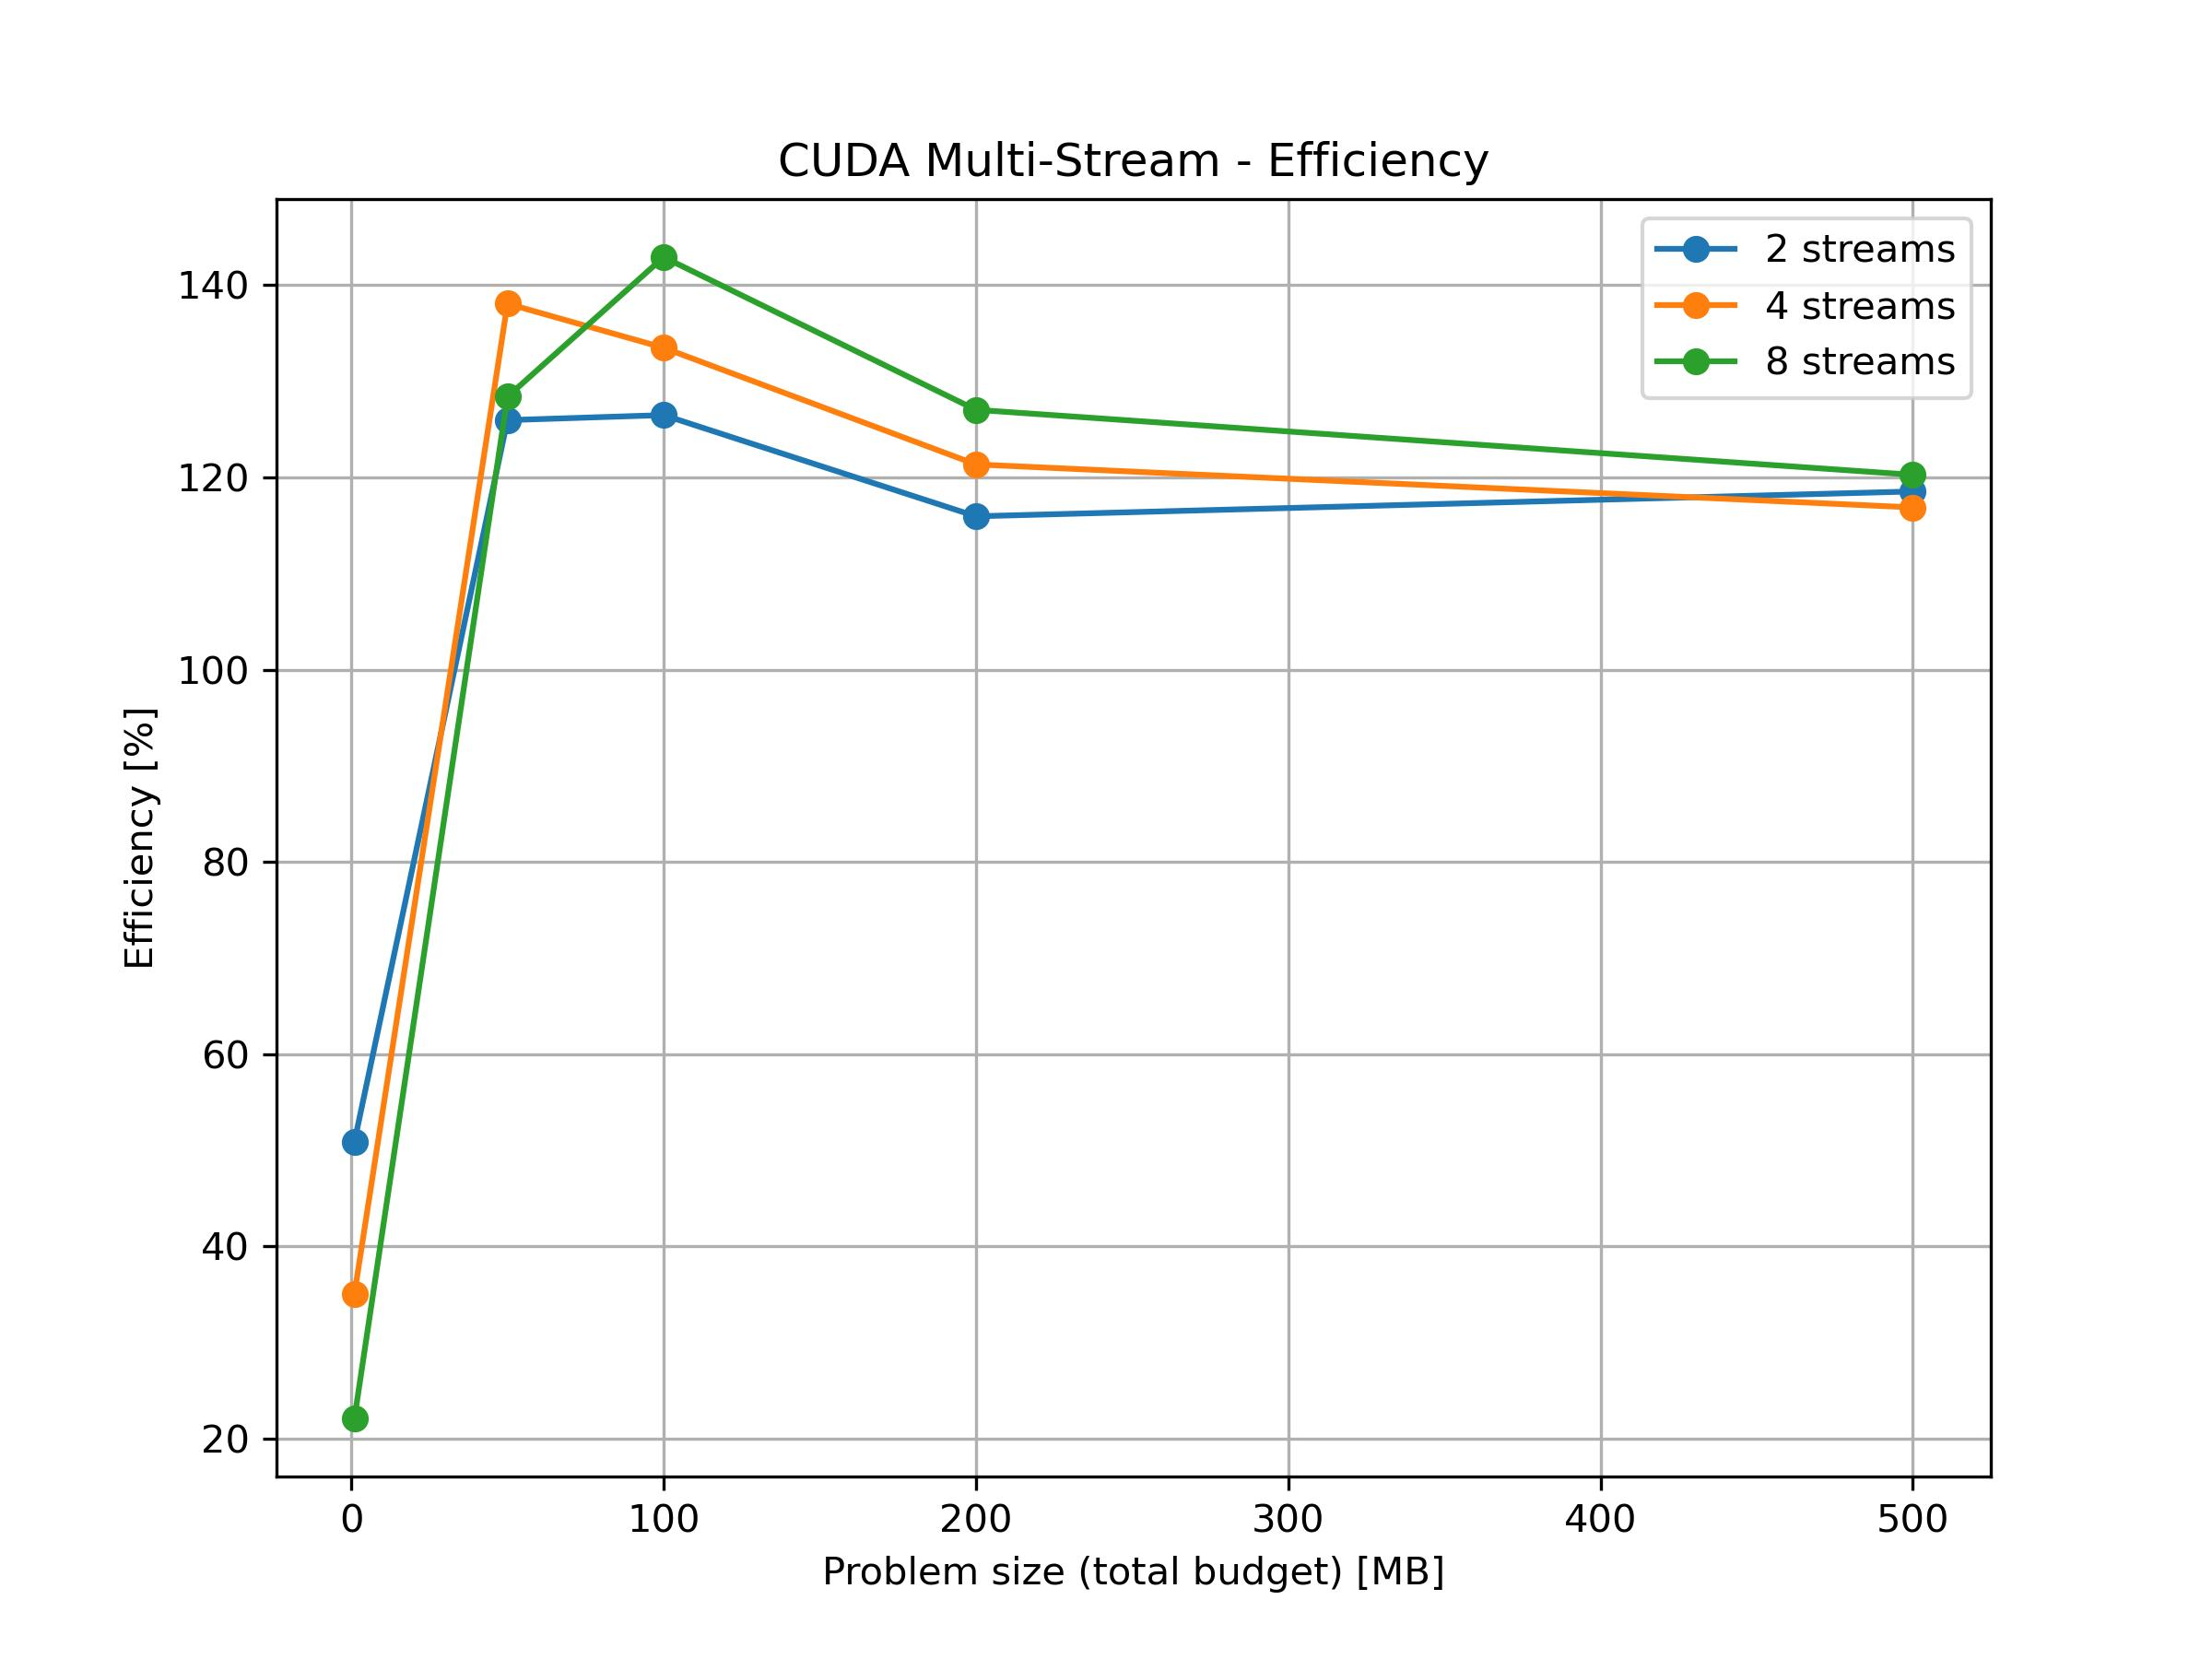
\includegraphics[width=\textwidth]{img/cuda_ms_plots/cuda_ms_efficiency.jpg}
					\caption{Efficiency CUDA MS}
					\label{fig:cuda_ms_efficiency}
				\end{minipage}
			\end{figure}
			
			\subsubsection*{Osservazioni}
				\begin{itemize}
						\item Le \textbf{copie D2H} restano consistenti e praticamente costanti al crescere degli stream (\(\sim 0.53\) s a 50 MB, \(\sim 1.49\) s a 100 MB, \(\sim 9.24\) s a 500 MB). Non sono il collo di bottiglia principale, ma non beneficiano del parallelismo tra stream.
						\item Il \textbf{kernel GPU} scala in modo inverso: a parità di input, più stream riducono leggermente il tempo medio del kernel (da 4.74 s a 4.65 s su 500 MB), per via di un miglior bilanciamento della concorrenza.
						\item \textbf{Throughput e speedup} migliorano con più stream. \\
						Ad esempio, a 100 MB si passa da 5.98 MB/s (2 stream) a 6.75 MB/s (8 stream), con speedup che cresce da \(1.26\times\) a \(1.43\times\).
						\item L’\textbf{efficienza} rimane alta (120–190\%), perché qui il calcolo dello speedup è rispetto al sequenziale CPU: la GPU anche in modalità multi-stream resta molto più veloce e la parallelizzazione per chunk non penalizza significativamente.
				\end{itemize}
		
		\subsection{Profiling della memoria}
			Con Nsight Compute su 500 MB e diverse configurazioni di stream:
			\begin{quote}
				\small
				2 stream: \texttt{time\_kernel\_gpu \(\approx 4.77\) s, time\_lcp\_cpu \(\approx 1.19\) s, time\_d2h \(\approx 9.20\) s, time\_compute\_pure \(\approx 5.96\) s, throughput \(\approx 4.00\) MB/s}.\\
				4 stream: \texttt{time\_kernel\_gpu \(\approx 4.88\) s, time\_lcp\_cpu \(\approx 1.18\) s, time\_d2h \(\approx 9.21\) s, time\_compute\_pure \(\approx 6.05\) s, throughput \(\approx 3.93\) MB/s}.\\
				8 stream: \texttt{time\_kernel\_gpu \(\approx 4.72\) s, time\_lcp\_cpu \(\approx 1.12\) s, time\_d2h \(\approx 9.17\) s, time\_compute\_pure \(\approx 5.84\) s, throughput \(\approx 4.07\) MB/s}.
			\end{quote}
			
			I valori sono coerenti con i dati aggregati (Tab.~\ref{tab:cuda-ms-times}). Le copie D2H restano sostanzialmente stabili e non mostrano overlapping tra stream; le differenze nei tempi di kernel spiegano le variazioni di throughput.
			
			\begin{figure}[H]
				\centering
				\begin{minipage}[t]{0.49\textwidth}
					\centering
					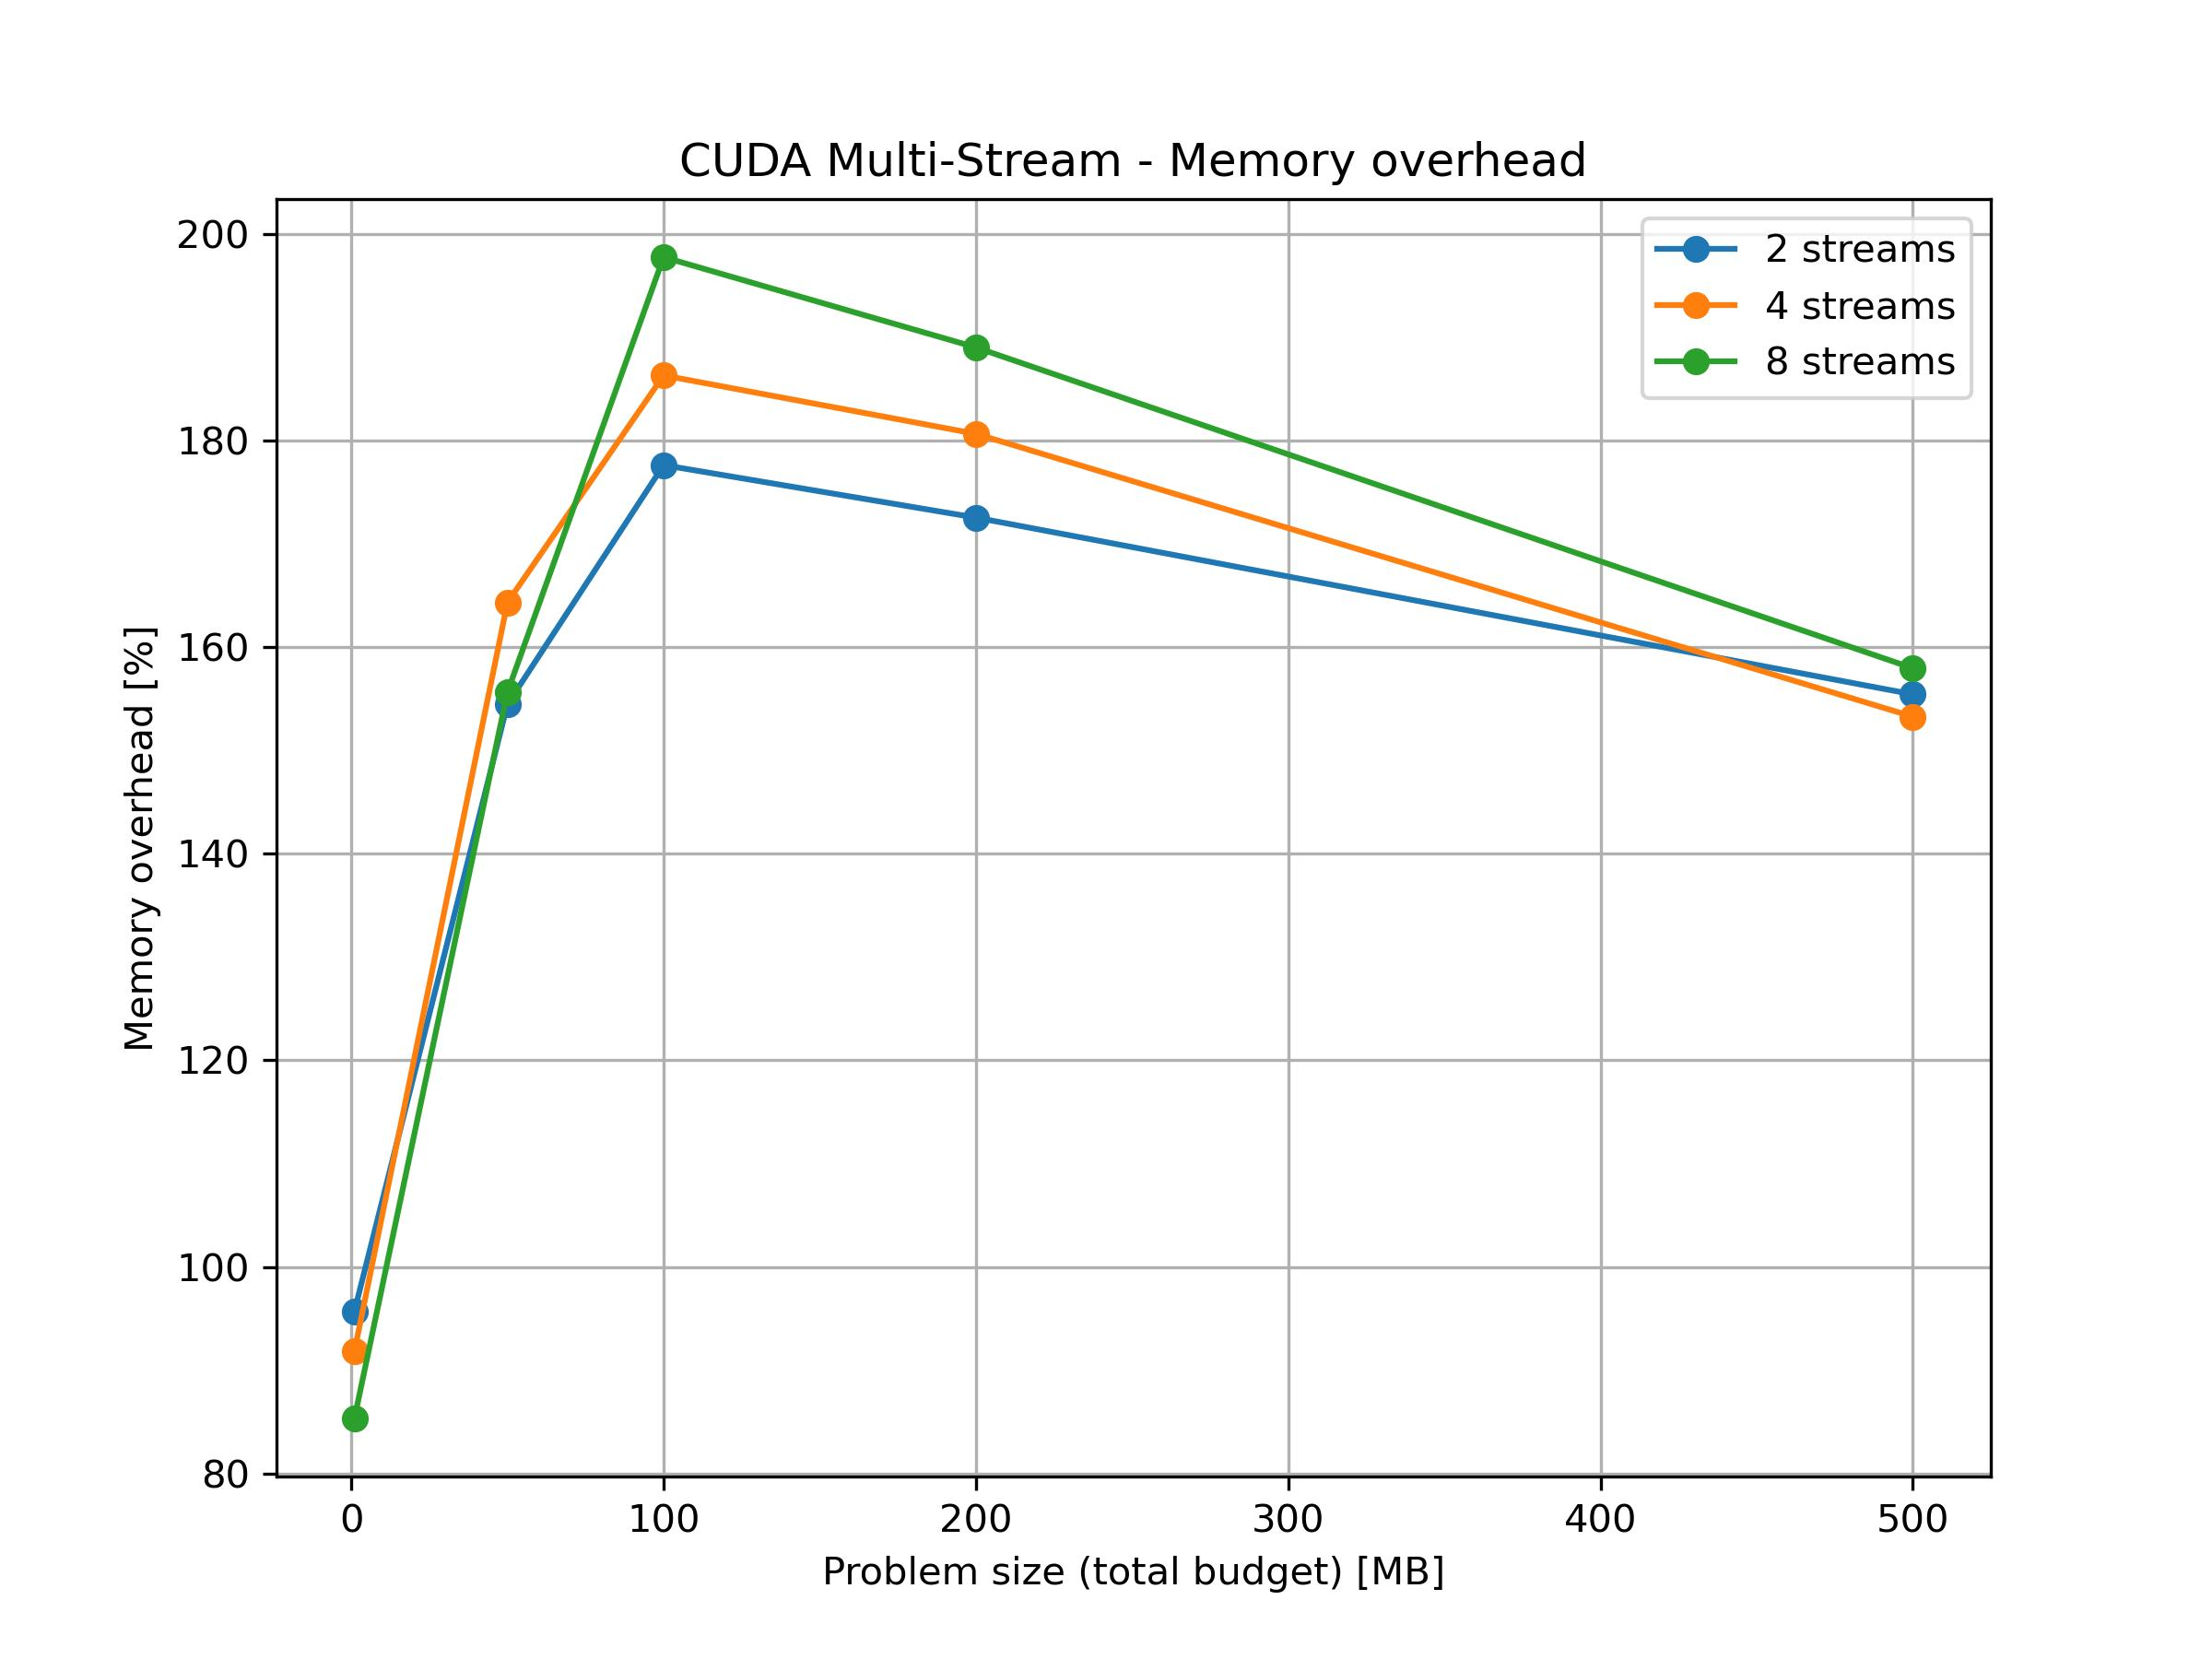
\includegraphics[width=\textwidth]{img/cuda_ms_plots/cuda_ms_memory_overhead.jpg}
					\caption{Memory overhead CUDA MS}
					\label{fig:cuda_ms_mem_overhead}
				\end{minipage}
				\hfill
				\begin{minipage}[t]{0.49\textwidth}
					\centering
					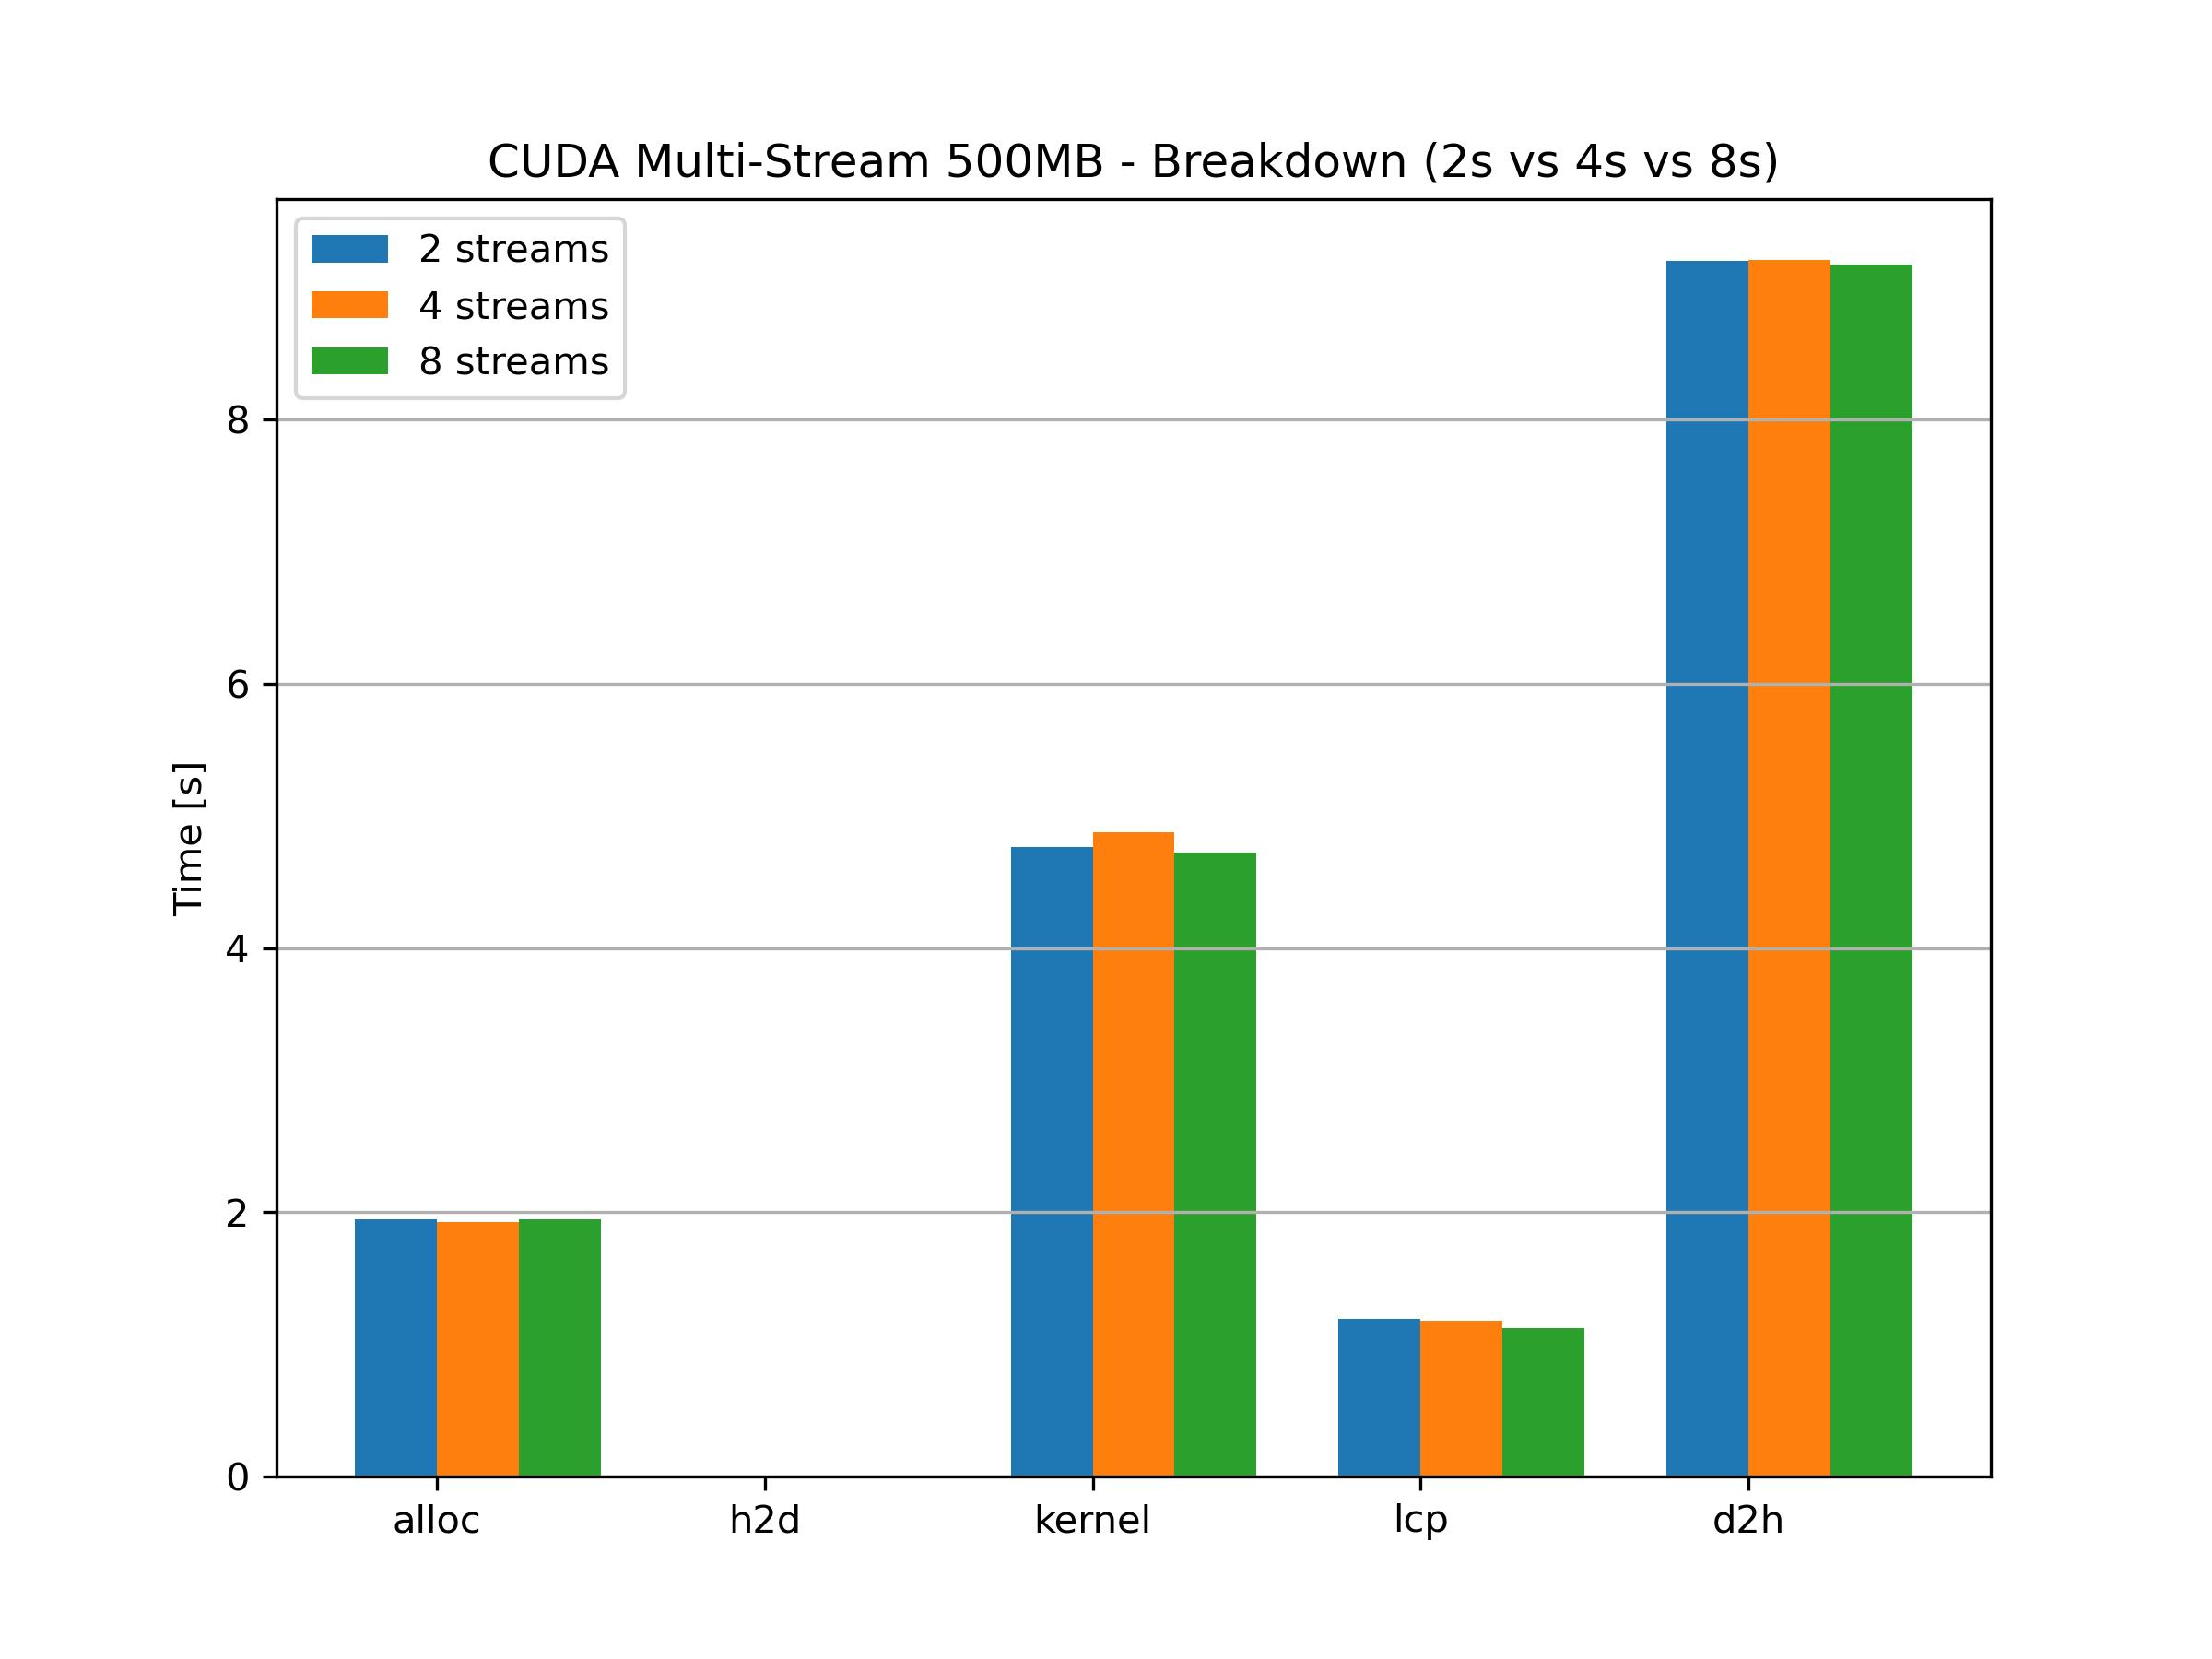
\includegraphics[width=\textwidth]{img/cuda_ms_plots/cuda_ms_breakdown_500MB.jpg}
					\caption{Breakdown CUDA MS (500MB, profili Nsight)}
					\label{fig:cuda_ms_breakdown}
				\end{minipage}
			\end{figure}
		
		\subsection{Confronto con single-stream}
			Rispetto alla versione single-stream, il multi-stream mostra un peggioramento evidente:
			il throughput cala di circa $2\times$ (es.\ a 100~MB da $\sim$15.8~MB/s a $\sim$6.8~MB/s)
			e lo speedup si riduce da oltre $3\times$ a circa $1.3{-}1.4\times$.
			Questo comportamento indica che l’overhead di gestione dei chunk e la serializzazione
			delle copie D2H annullano i potenziali benefici del parallelismo per stream.
			In altre parole, la versione multi-stream è meno efficiente del single-stream
			nelle condizioni sperimentate.
		
		\subsection{Conclusioni}
			La versione \emph{multi-stream} è \textbf{compute-bound}, con throughput e speedup che migliorano leggermente al crescere degli stream.
			Per sfruttare appieno il modello servirebbe ridurre il costo delle D2H (pinned memory, batching delle copie) così da ottenere un vero overlap con i kernel.
	
	\section{Confronto complessivo tra modelli}
		Per fornire una visione sintetica e chiara, i grafici finali confrontano soltanto le migliori configurazioni per ciascun paradigma di parallelizzazione, evitando di riportare tutte le combinazioni (che renderebbero i grafici troppo affollati). \\
		In particolare sono stati selezionati:
		\begin{itemize}
			\item \textbf{Sequenziale (baseline)};
			\item \textbf{OpenMP}: configurazione a 8 thread (\texttt{omp\_summary\_8.csv});
			\item \textbf{MPI}: configurazione a 8 ranks (\texttt{mpi\_summary\_8.csv});
			\item \textbf{MPI+OpenMP}: configurazione 8 ranks $\times$ 2 thread per rank (\texttt{mpi\_omp\_summary\_8r\_2t.csv});
			\item \textbf{CUDA (single-stream)}: \texttt{cuda\_summary.csv};
			\item \textbf{CUDA (multi-stream)}: configurazione a 8 stream (\texttt{cuda\_ms\_summary.csv}).
		\end{itemize}
		I plot mostrano l’andamento dei tempi, del throughput e dello speedup rispetto alla baseline sequenziale, consentendo un confronto diretto tra i modelli più efficienti per ciascuna classe di parallelizzazione.
		
		\begin{figure}[H]
			\centering
			\includesvg[width=0.8\textwidth]{img/overall_plots/overall_times.svg}
			\caption{Tempi di esecuzione}
			\label{fig:summary-times}
		\end{figure}
		
		\begin{figure}[H]
			\centering
			\begin{minipage}[t]{0.49\textwidth}
				\centering
				\includesvg[width=\textwidth]{img/overall_plots/overall_throughput.svg}
				\caption{Throughput (MB/s)}
				\label{fig:summary-throughput}
			\end{minipage}
			\hfill
			\begin{minipage}[t]{0.49\textwidth}
				\centering
				\includesvg[width=\textwidth]{img/overall_plots/overall_speedup.svg}
				\caption{Speedup}
				\label{fig:summary-speedup}
			\end{minipage}
		\end{figure}
		
		\begin{figure}[H]
			\begin{minipage}[t]{0.49\textwidth}
				\centering
				\includesvg[width=\textwidth]{img/overall_plots/overall_efficiency.svg}
				\caption{Efficiency}
				\label{fig:summary-efficiency}
			\end{minipage}
			\hfill
			\begin{minipage}[t]{0.49\textwidth}
				\centering
				\includesvg[width=\textwidth]{img/overall_plots/overall_memory_overhead.svg}
				\caption{Memory overhead ratio (\%)}
				\label{fig:summary-memory-overhead}
			\end{minipage}
		\end{figure}
		
		\begin{figure}[H]
			\centering
			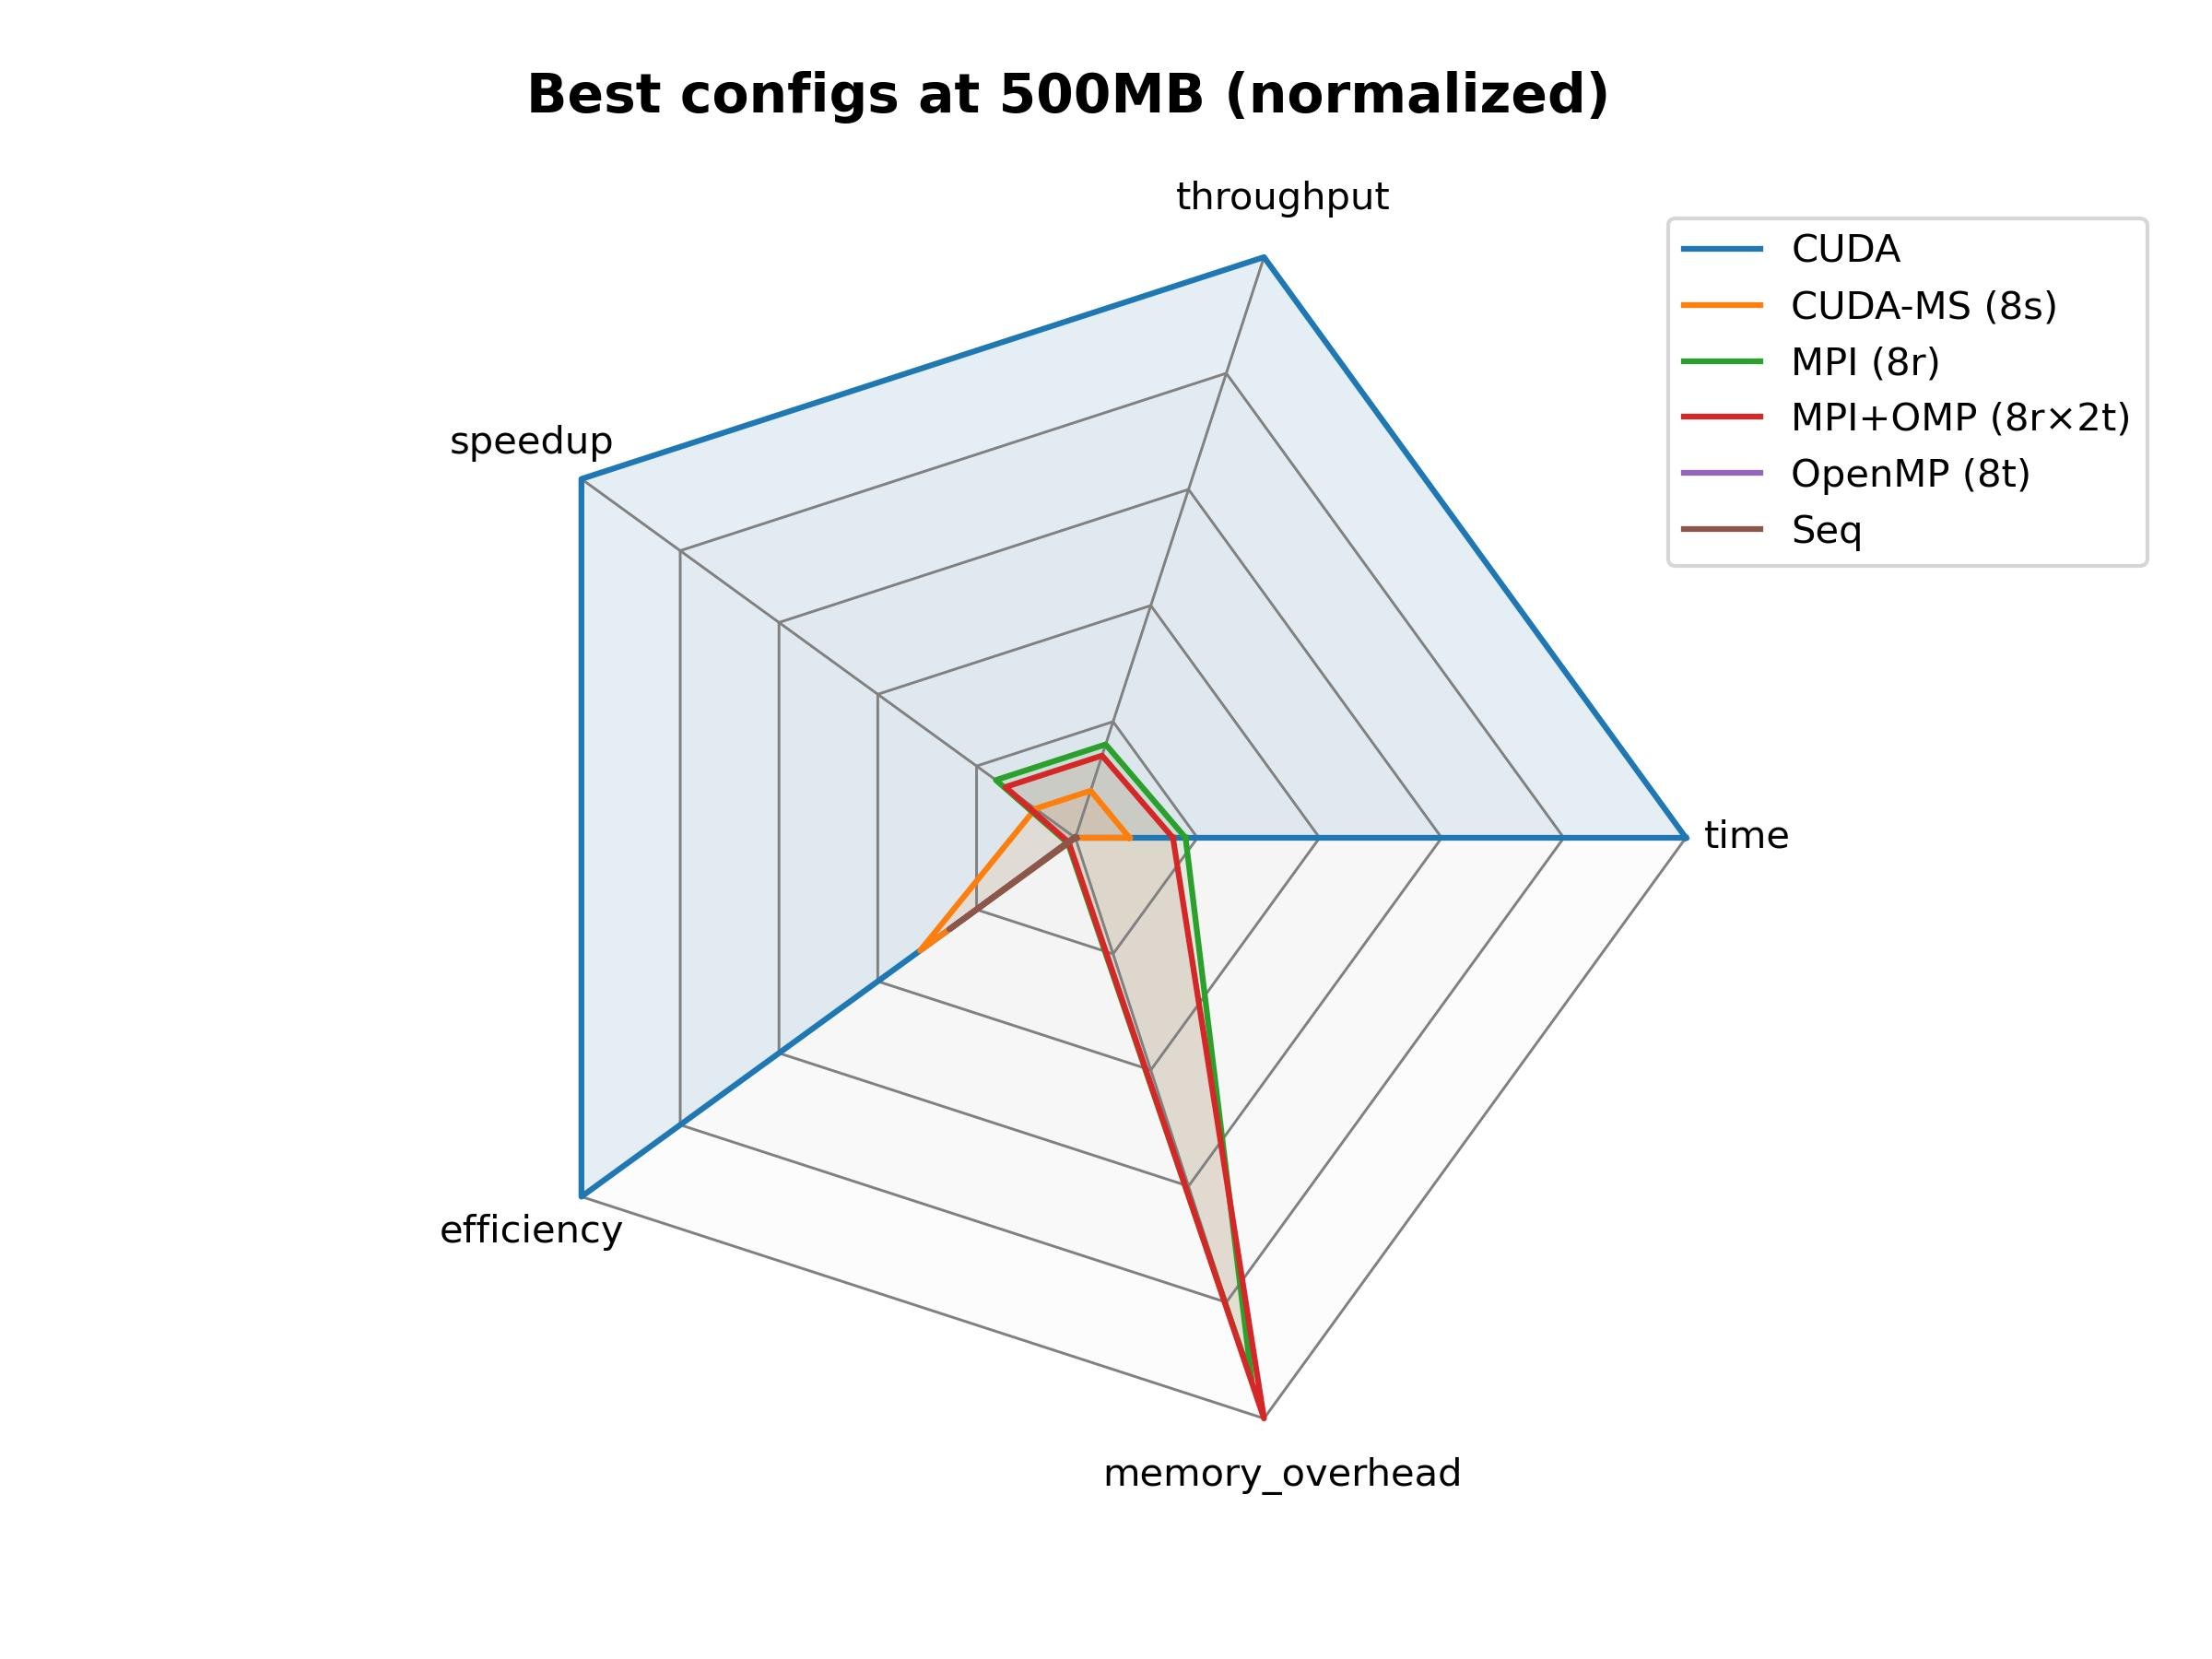
\includegraphics[width=0.5\textwidth]{img/overall_plots/overall_radar_500MB.jpg}
			\caption{Radar chart}
			\label{Radar chart}
		\end{figure}

    \listoftables
    \listoffigures

\end{document}